\documentclass[12pt,oneside]{book}

\usepackage{fontspec}
\usepackage{polyglossia}
\setdefaultlanguage{polish}

\setmainfont{Linux Libertine O}

\usepackage{geometry}
\geometry{a4paper, margin=2.5cm}

\usepackage{float}
\let\origfigure\figure
\let\endorigfigure\endfigure
\renewenvironment{figure}[1][H]{\origfigure[#1]}{\endorigfigure}

\usepackage{graphicx}
\makeatletter
\def\maxwidth{\ifdim\Gin@nat@width>\linewidth\linewidth\else\Gin@nat@width\fi}
\def\maxheight{\ifdim\Gin@nat@height>\textheight\textheight\else\Gin@nat@height\fi}
\makeatother
\setkeys{Gin}{width=\maxwidth,height=\maxheight,keepaspectratio}
\let\origincludegraphics\includegraphics
\renewcommand{\includegraphics}[2][]{%
  \par\noindent\makebox[\linewidth][c]{\origincludegraphics[#1]{#2}}\par\vspace{\baselineskip}%
}

\usepackage{longtable,booktabs,array,calc}
\usepackage{newunicodechar}
\newunicodechar{✓}{\checkmark}
\newunicodechar{✗}{$\times$}
\usepackage{amssymb}

\usepackage{titlesec}
\titleformat{\section}
  {\normalfont\huge\bfseries\centering}
  {}
  {0pt}
  {}
\titleformat{\subsection}
  {\normalfont\Large\bfseries\raggedright}
  {}
  {0pt}
  {}
\titleformat{\subsubsection}
  {\normalfont\large\centering}
  {}
  {0pt}
  {}

\usepackage{fancyhdr}
\pagestyle{fancy}
\fancyhead{}
\fancyhead[L]{Sylwetki uzbrojenia Federacji Rosyjskiej}
\fancyhead[R]{\nouppercase{\rightmark}}
\fancyfoot[C]{\thepage}
\renewcommand{\sectionmark}[1]{\markright{#1}}

\usepackage{setspace}
\setstretch{1.1}

\hyphenpenalty=10000
\exhyphenpenalty=10000
\pretolerance=10000
\tolerance=2000
\emergencystretch=1.5em

\usepackage[skip=5pt plus 2pt, indent=0pt]{parskip}
\usepackage{enumitem}
\setlist{nosep}

\usepackage{tocloft}
\renewcommand{\cfttoctitlefont}{\normalfont\Large}
\renewcommand{\cftsecfont}{\normalfont\fontsize{11pt}{13pt}\selectfont}
\renewcommand{\cftsecpagefont}{\normalfont\fontsize{11pt}{13pt}\selectfont}

\usepackage{hyperref}
\usepackage{etoolbox}
\usepackage{needspace}
\newif\iffirstsection
\firstsectiontrue
\pretocmd{\section}{%
  \iffirstsection
    \global\firstsectionfalse
  \else
    \clearpage
  \fi
}{}{}
\pretocmd{\subsection}{\Needspace{8\baselineskip}}{}{}
\pretocmd{\subsubsection}{\Needspace{7\baselineskip}}{}{}

\providecommand{\tightlist}{%
  \setlength{\itemsep}{0pt}\setlength{\parskip}{0pt}}

\title{Sylwetki uzbrojenia Federacji Rosyjskiej}
\author{Grzegorz KASZUBA}
\date{3 kwietnia 2026}

\begin{document}

\frontmatter
\begin{titlepage}
    \centering
    \vspace*{1cm}
      {\huge\bfseries Sylwetki uzbrojenia Federacji Rosyjskiej \par}
    \vspace{1cm}
    {\Large Grzegorz KASZUBA \par}
    \vspace{0.3cm}
    {\normalsize \href{http://buymeacoffee.com/uirapuru}{http://buymeacoffee.com/uirapuru} \par}
    \vfill
    {\large 3 kwietnia 2026 \par}
\end{titlepage}

  \clearpage
  \thispagestyle{empty}
  
  \clearpage
\setcounter{tocdepth}{1}
\tableofcontents

\clearpage
\pagenumbering{arabic}
\setcounter{page}{1}
\setcounter{secnumdepth}{-1}

\section{Czołg średni T-55}\label{czoux142g-ux15bredni-t-55}

\subsubsection{T-55 Medium Tank \textbar{} Т-55 Средний
танк}\label{t-55-medium-tank-ux442-55-ux441ux440ux435ux434ux43dux438ux439-ux442ux430ux43dux43a}

\begin{figure}
\centering
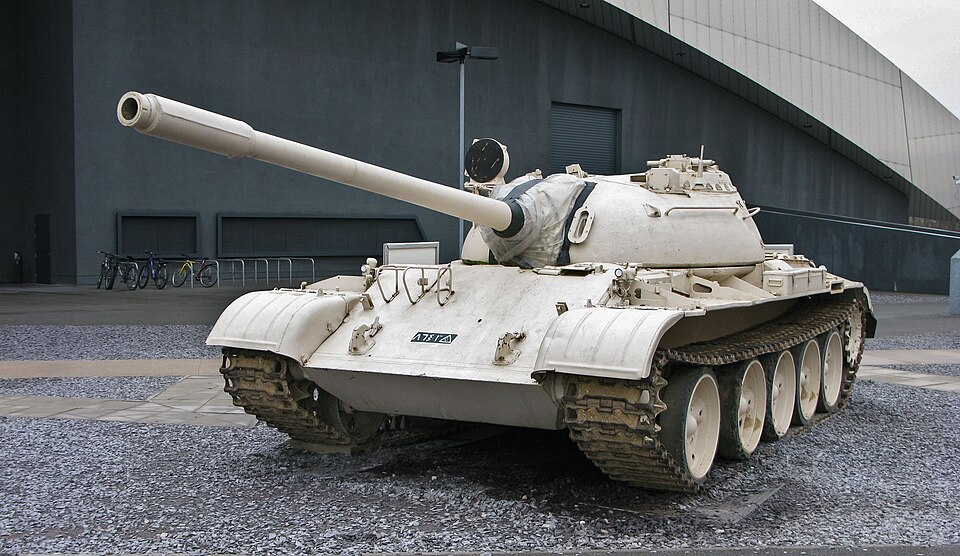
\includegraphics{../images/czolgi/t-55_1.jpg}
\caption{T-55 --- widok z boku}
\end{figure}

\begin{center}\rule{0.5\linewidth}{0.5pt}\end{center}

\subsection{Opis}\label{opis}

T-55 to radziecki czołg średni przyjęty na uzbrojenie Armii Radzieckiej
8 maja 1958 roku, będący głęboko zmodernizowaną wersją T-54. Jest jednym
z najliczniej produkowanych czołgów w historii --- szacuje się, że
powstało ponad 96 000 egzemplarzy różnych wariantów. Był standardowym
czołgiem Układu Warszawskiego przez lata 60. i 70. XX wieku i trafił do
armii ponad 50 krajów. Choć dawno wycofany z aktywnej służby, od wiosny
2023 roku Rosja wyciągała T-55 z głębokich rezerw magazynowych i
wysyłała na front w Ukrainie jako mobilne działa wsparcia ogniowego.

\subsection{Dane techniczne}\label{dane-techniczne}

\begin{longtable}[]{@{}
  >{\raggedright\arraybackslash}p{(\columnwidth - 2\tabcolsep) * \real{0.5263}}
  >{\raggedright\arraybackslash}p{(\columnwidth - 2\tabcolsep) * \real{0.4737}}@{}}
\toprule\noalign{}
\begin{minipage}[b]{\linewidth}\raggedright
Parametr
\end{minipage} & \begin{minipage}[b]{\linewidth}\raggedright
Wartość
\end{minipage} \\
\midrule\noalign{}
\endhead
\bottomrule\noalign{}
\endlastfoot
Typ & Czołg średni \\
Kraj produkcji & ZSRR \\
Rok wprowadzenia & 1958 \\
Masa bojowa & ok. 36--36,5 t \\
Długość (z działem) & 9,00 m \\
Szerokość & 3,27--3,37 m \\
Wysokość & 2,35--2,40 m \\
Uzbrojenie główne & Armata 100 mm D-10T2S (gwintowana) \\
Uzbrojenie dodatkowe & KM 7,62 mm PKT (sprzężony), WKCKM 12,7 mm DSzKM
(plot.) \\
Silnik & W-55 diesel, 580 KM \\
Prędkość maks. (droga) & 50--51 km/h \\
Zasięg & 325--500 km (do 610 km z bak. dod.) \\
Załoga & 4 osoby (dowódca, działonowy, ładowniczy, kierowca) \\
Pancerz czoła wieży & do 203--205 mm (odlewany) \\
\end{longtable}

\subsection{Charakterystyczne cechy
rozpoznawcze}\label{charakterystyczne-cechy-rozpoznawcze}

\begin{quote}
Jak odróżnić T-55 od T-54, T-62 i innych czołgów:
\end{quote}

\begin{itemize}
\tightlist
\item
  \textbf{Wyraźna przerwa między 1. a 2. kołem nośnym:} największy
  odstęp między kołami jest z przodu pojazdu --- odwrotnie niż w T-62,
  gdzie przerwy rosną ku tyłowi
\item
  \textbf{Półsferyczna, zaokrąglona wieża bez kopuły wentylatora:} w
  odróżnieniu od T-54 brak małej kopułki z prawej strony dachu wieży
\item
  \textbf{Brak otworu strzelniczego w przedniej płycie kadłuba:} T-54
  miał nieruchomy km w dziobie; T-55 nie --- środek czołowej płyty jest
  gładki
\item
  \textbf{Rura wydechowa widoczna na lewym tylnym błotniku:}
  charakterystyczny element zewnętrzny
\item
  \textbf{Armata 100 mm z przedmuchiwaczem bliżej wylotu lufy:} w
  odróżnieniu od T-62, którego 115 mm armata ma przedmuchiwacz w połowie
  lufy
\item
  \textbf{Brak fartuchów bocznych} (ekranów gumowo-metalowych) w wersji
  bazowej
\end{itemize}

\subsection{Ciekawostka}\label{ciekawostka}

\begin{quote}
T-55 to najliczniej produkowany czołg w historii --- ponad 96 000 sztuk.
Był też pierwszym czołgiem wyposażonym w system ochrony przed bronią
masowego rażenia (PAZ). W wojnie w Ukrainie Rosjanie używali go nie jako
czołgu liniowego, lecz jako ``mobilnej artylerii'' --- wyciągniętej z
magazynów po ogromnych stratach nowoczesnego sprzętu. Ukraińcy zdobyli
T-55 z cokołu pomnika w Mariupolu i użyli go jako bunkier podczas obrony
Azowstalu.
\end{quote}

\section{Czołg podstawowy T-62}\label{czoux142g-podstawowy-t-62}

\subsubsection{T-62 Main Battle Tank \textbar{} Т-62 Основной боевой
танк}\label{t-62-main-battle-tank-ux442-62-ux43eux441ux43dux43eux432ux43dux43eux439-ux431ux43eux435ux432ux43eux439-ux442ux430ux43dux43a}

\begin{figure}
\centering
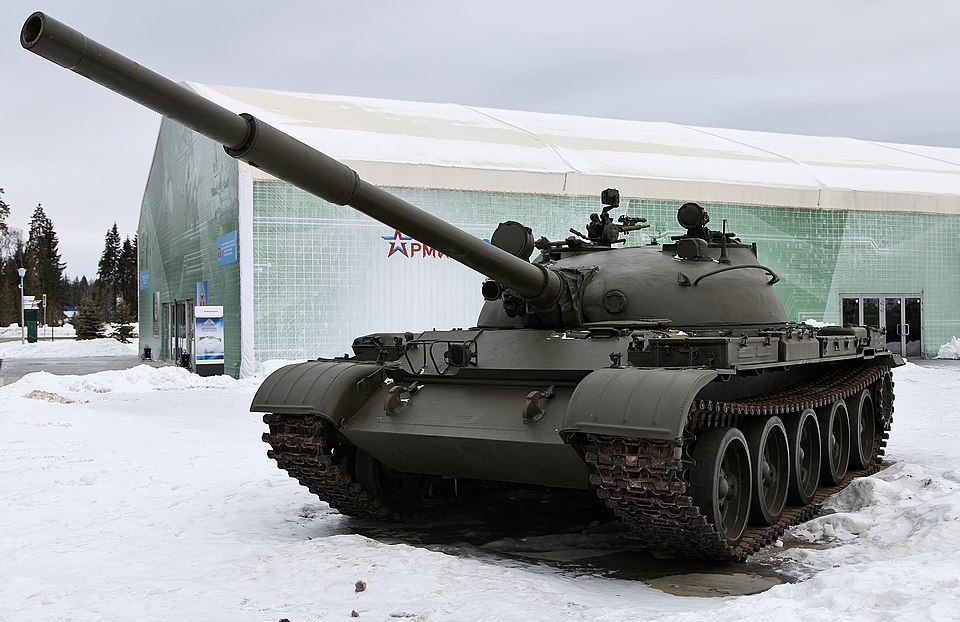
\includegraphics{../images/czolgi/t-62_1.jpg}
\caption{T-62 --- widok z boku}
\end{figure}

\begin{center}\rule{0.5\linewidth}{0.5pt}\end{center}

\subsection{Opis}\label{opis-1}

T-62 to radziecki czołg podstawowy wprowadzony do służby w lipcu 1961
roku. Jest historycznie przełomowy --- jako pierwszy seryjnie
produkowany czołg na świecie uzbrojony w armatę gładkolufową, zdolną do
strzelania pociskami podkalibrowymi stabilizowanymi brzechwowo (APFSDS).
Powstał jako ewolucja T-55, z którym dzieli wiele elementów konstrukcji.
Produkowany w ZSRR do 1975 roku (ok. 22 000 egzemplarzy), trafił do
blisko 40 krajów. Od maja 2022 roku Rosja wyciąga T-62 z głębokich
rezerw i wysyła na front w Ukrainie.

\subsection{Dane techniczne}\label{dane-techniczne-1}

\begin{longtable}[]{@{}
  >{\raggedright\arraybackslash}p{(\columnwidth - 2\tabcolsep) * \real{0.5263}}
  >{\raggedright\arraybackslash}p{(\columnwidth - 2\tabcolsep) * \real{0.4737}}@{}}
\toprule\noalign{}
\begin{minipage}[b]{\linewidth}\raggedright
Parametr
\end{minipage} & \begin{minipage}[b]{\linewidth}\raggedright
Wartość
\end{minipage} \\
\midrule\noalign{}
\endhead
\bottomrule\noalign{}
\endlastfoot
Typ & Czołg podstawowy \\
Kraj produkcji & ZSRR \\
Rok wprowadzenia & 1961 \\
Masa bojowa & ok. 37--40 t \\
Długość (z działem) & 9,34 m \\
Szerokość & 3,30 m \\
Wysokość & 2,28--2,40 m \\
Uzbrojenie główne & Armata 115 mm 2A20 U-5TS ``Mołot'' (gładkolufowa) \\
Uzbrojenie dodatkowe & KM 7,62 mm PKT (sprzężony), WKCKM 12,7 mm DSzK
(plot.) \\
Silnik & W-55V diesel, 580 KM \\
Prędkość maks. (droga) & 50 km/h \\
Zasięg & 450 km (do 650 km z bak. dod.) \\
Załoga & 4 osoby (dowódca, działonowy, ładowniczy, kierowca) \\
Pancerz czoła wieży & 214--242 mm (odlewany) \\
\end{longtable}

\subsection{Charakterystyczne cechy
rozpoznawcze}\label{charakterystyczne-cechy-rozpoznawcze-1}

\begin{quote}
Jak odróżnić T-62 od T-55 i T-72:
\end{quote}

\begin{itemize}
\tightlist
\item
  \textbf{Przerwy między kołami rosną ku tyłowi:} trzy ostatnie pary kół
  nośnych są rozmieszczone szerzej niż przednie --- odwrotnie niż w
  T-55, gdzie największa przerwa jest z przodu
\item
  \textbf{Jajowata, spłaszczona wieża bez wyraźnych krawędzi:} bardziej
  owalna niż wieża T-55; wyraźnie różna od kanciastej wieży T-72
\item
  \textbf{Klapka wyrzutnika łusek z tyłu wieży:} mały prostokątny właz
  po lewej lub prawej stronie tylnej ściany wieży --- unikalna cecha
  T-62 (łuski 115 mm są wyrzucane automatycznie na zewnątrz)
\item
  \textbf{Przedmuchiwacz gazów w połowie lufy:} charakterystyczne
  zgrubienie lufy dokładnie pośrodku jej długości; w T-55 z armatą 100
  mm przedmuchiwacz jest bliżej wylotu
\item
  \textbf{Brak fartuchów bocznych} w wersji bazowej (pojawiają się
  dopiero w T-62M)
\end{itemize}

\subsection{Ciekawostka}\label{ciekawostka-1}

\begin{quote}
T-62 był pierwszym na świecie seryjnym czołgiem z armatą gładkolufową.
Ze względu na ogromne rozmiary łusek 115 mm zastosowano unikalny automat
wyrzutowy --- po strzale tylna klapka wieży otwierała się i gorąca łuska
wylatywała na zewnątrz. W 1969 roku zdobyczny T-62 (utopiony przez
Chińczyków w rzece Ussuri) posłużył im jako baza technologiczna do
stworzenia własnego czołgu Typ 69. W Ukrainie Rosjanie montują na
wieżach T-62 improwizowane klatki spawane z prętów stalowych, mające
chronić przed dronami i pociskami kumulacyjnymi.
\end{quote}

\section{Czołg podstawowy T-62M}\label{czoux142g-podstawowy-t-62m}

\subsubsection{T-62M Main Battle Tank \textbar{} Т-62М Основной боевой
танк}\label{t-62m-main-battle-tank-ux442-62ux43c-ux43eux441ux43dux43eux432ux43dux43eux439-ux431ux43eux435ux432ux43eux439-ux442ux430ux43dux43a}

\begin{figure}
\centering
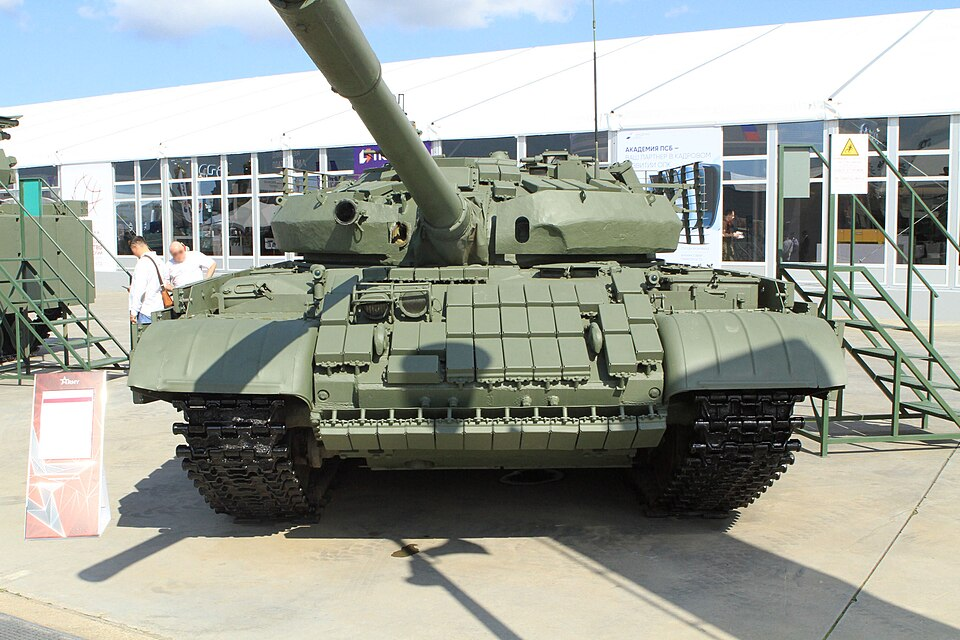
\includegraphics{../images/czolgi/t-62m_1.jpg}
\caption{T-62M --- widok z boku}
\end{figure}

\begin{center}\rule{0.5\linewidth}{0.5pt}\end{center}

\subsection{Opis}\label{opis-2}

T-62M to modernizacja czołgu T-62 przeprowadzona w 1983 roku, mająca na
celu przedłużenie żywotności bojowej przestarzałej platformy.
Wprowadzono dodatkowy pancerz pasywny BDD (bloki kompozytowe na wieży i
kadłubie), nowy system kierowania ogniem ``Wołna'' z dalmierzem
laserowym, mocniejszy silnik W-55U (620 KM) oraz możliwość odpalania
przeciwpancernych pocisków kierowanych 9M117 Bastion przez lufę armaty.
Wariant z pancerzem reaktywnym Kontakt-1 (z 1985 r.) oznaczany jest jako
\textbf{T-62MW}. T-62M pojawił się w Afganistanie i jest szeroko
stosowany przez Rosję w wojnie w Ukrainie od 2022 roku.

\subsection{Dane techniczne}\label{dane-techniczne-2}

\begin{longtable}[]{@{}
  >{\raggedright\arraybackslash}p{(\columnwidth - 2\tabcolsep) * \real{0.5263}}
  >{\raggedright\arraybackslash}p{(\columnwidth - 2\tabcolsep) * \real{0.4737}}@{}}
\toprule\noalign{}
\begin{minipage}[b]{\linewidth}\raggedright
Parametr
\end{minipage} & \begin{minipage}[b]{\linewidth}\raggedright
Wartość
\end{minipage} \\
\midrule\noalign{}
\endhead
\bottomrule\noalign{}
\endlastfoot
Typ & Czołg podstawowy (modernizacja T-62) \\
Kraj produkcji & ZSRR \\
Rok modernizacji & 1983 \\
Masa bojowa & ok. 40--41,5 t (zwiększona przez pancerz BDD) \\
Uzbrojenie główne & Armata 115 mm 2A20 U-5TS (gładkolufowa) \\
Uzbrojenie dodatkowe & KM 7,62 mm PKT, WKCKM 12,7 mm DSzK; rakiety 9M117
Bastion \\
Silnik & W-55U diesel, 620 KM \\
System KO & ``Wołna'' z dalmierzem laserowym KTD-1/2 i przelicznikiem
balistycznym \\
Pancerz dodatkowy & BDD (pasywny kompozyt) na wieży i glacis; T-62MW:
ERA Kontakt-1 \\
Załoga & 4 osoby (dowódca, działonowy, ładowniczy, kierowca) \\
\end{longtable}

\subsection{Charakterystyczne cechy
rozpoznawcze}\label{charakterystyczne-cechy-rozpoznawcze-2}

\begin{quote}
Jak odróżnić T-62M od bazowego T-62:
\end{quote}

\begin{itemize}
\tightlist
\item
  \textbf{Dwa podkowiaste bloki BDD na wieży:} półokrągłe, masywne bloki
  pancerza kompozytowego okalające armatę z obu stron --- zmieniają
  sylwetkę wieży nie do poznania; usunięto też poręcze dla piechoty
\item
  \textbf{Osłona termiczna lufy:} gruba, rurowa osłona ciągnie się
  wzdłuż lufy armaty --- w bazowym T-62 lufa jest ``gołą'' rurą
\item
  \textbf{Prostokątna skrzynka dalmierza laserowego nad jarzmem armaty:}
  widoczny z zewnątrz pancerny pojemnik tuż nad podstawą lufy
\item
  \textbf{Gumowo-metalowe fartuchy boczne:} ekrany wzdłuż gąsienic,
  których brak w T-62 bazowym
\item
  \textbf{T-62MW:} dodatkowo prostokątne kostki ERA Kontakt-1
  przykrywające glacis i wieżę (identyczne jak na T-72B)
\item
  \textbf{Wyrzutnie granatów dymnych:} skupisko 2×4 wyrzutni na tylnej
  ścianie wieży (po prawej stronie)
\end{itemize}

\subsection{Ciekawostka}\label{ciekawostka-2}

\begin{quote}
Pancerz BDD tak skutecznie wzmocnił ochronę T-62M, że czołek wieży stał
się niemal równorzędny z wczesnymi wariantami T-64A i T-72 Ural. Gdy
wywiad USA po raz pierwszy zaobserwował T-62M w Afganistanie, nie znając
oficjalnego oznaczenia, nadał mu własny kod: \textbf{T-62E}. W Ukrainie
zdobyczne T-62M bywają przebudowywane przez Ukraińców --- zdejmują wieżę
i instalują wieżę z BWP-2 z działkiem 30 mm, tworząc improwizowany
ciężki wóz bojowy piechoty.
\end{quote}

\section{Czołg podstawowy T-72}\label{czoux142g-podstawowy-t-72}

\subsubsection{T-72 Main Battle Tank \textbar{} Т-72 Основной боевой
танк}\label{t-72-main-battle-tank-ux442-72-ux43eux441ux43dux43eux432ux43dux43eux439-ux431ux43eux435ux432ux43eux439-ux442ux430ux43dux43a}

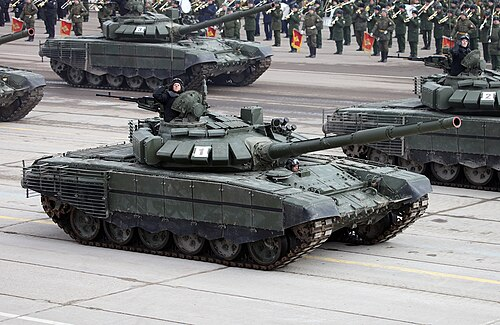
\includegraphics{../images/czolgi/t-72_1.jpg}
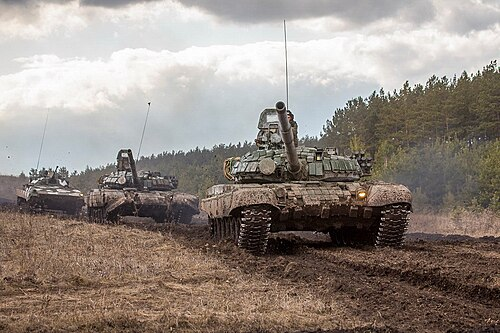
\includegraphics{../images/czolgi/t-72_2.jpg}

\begin{center}\rule{0.5\linewidth}{0.5pt}\end{center}

\subsection{Opis}\label{opis-3}

T-72 to radziecki czołg podstawowy opracowany w latach 60. XX wieku jako
tańsza i prostsza alternatywa dla T-64. Wszedł na wyposażenie Armii
Radzieckiej w 1973 roku i stał się jednym z najszerzej produkowanych
czołgów w historii --- wyprodukowano ponad 20 000 egzemplarzy różnych
wariantów. Służy do dziś w armiach ponad 40 krajów i jest podstawowym
czołgiem Wojsk Lądowych Federacji Rosyjskiej, regularnie modernizowany
do wersji T-72B3M. Brał udział w niemal wszystkich konfliktach zbrojnych
od lat 80. XX wieku po dzień dzisiejszy, w tym w wojnie w Ukrainie.

\subsection{Dane techniczne}\label{dane-techniczne-3}

\begin{longtable}[]{@{}ll@{}}
\toprule\noalign{}
Parametr & Wartość \\
\midrule\noalign{}
\endhead
\bottomrule\noalign{}
\endlastfoot
Typ & Czołg podstawowy \\
Kraj produkcji & ZSRR / Rosja \\
Rok wprowadzenia & 1973 \\
Masa bojowa & 41,5--46 t (zależnie od wersji) \\
Długość (z działem) & 9,53 m \\
Szerokość & 3,59 m \\
Wysokość & 2,23 m \\
Uzbrojenie główne & Armata 125 mm 2A46M (gładkolufowa) \\
Uzbrojenie dodatkowe & CKM 7,62 mm PKT, CKM 12,7 mm NSVT \\
Silnik & W-84MS diesel, 840 KM (T-72B3: 1130 KM) \\
Prędkość maks. (droga) & 60--70 km/h \\
Zasięg & 460--700 km \\
Załoga & 3 osoby (dowódca, działonowy, kierowca) \\
Pancerz czoła wieży & kompozytowy + reaktywny ERA Kontakt-5 \\
\end{longtable}

\subsection{Charakterystyczne cechy
rozpoznawcze}\label{charakterystyczne-cechy-rozpoznawcze-3}

\begin{quote}
Jak odróżnić T-72 od T-80 i T-90:
\end{quote}

\begin{itemize}
\tightlist
\item
  \textbf{Zaokrąglona, niska wieża:} charakterystyczny ``grzyb'' ---
  wieża T-72 jest niższa i bardziej zaokrąglona niż wieża T-80, bez
  ostrego podciętego profilu
\item
  \textbf{Brak osłony lufy (termicznej):} starsze warianty T-72 mają
  lufę bez charakterystycznej czarnej rury izolacyjnej; nowsze T-72B3
  mają ją, ale cieńszą niż T-90M
\item
  \textbf{Koła jezdne z dużymi otworami:} T-72 ma 6 dużych kół jezdnych
  z wyraźnymi okrągłymi otworami odciążającymi --- T-80 ma koła pełne
  lub z mniejszymi otworami
\item
  \textbf{Napęd gąsienicowy bez fartucha bocznego (lub z krótkim):}
  starsze T-72 nie mają pełnych gumowych fartuchów bocznych, widać górną
  część gąsienicy
\item
  \textbf{ERA Kontakt-1 lub Kontakt-5:} T-72B pokryty jest
  charakterystycznymi prostokątnymi blokami pancerza reaktywnego na
  czole kadłuba i wieży
\item
  \textbf{Silnik diesla --- charakterystyczny dym:} T-72 jest napędzany
  silnikiem Diesla, przy przyspieszeniu wydziela czarny lub szarawy dym;
  T-80 (turbina gazowa) praktycznie nie dymuje
\end{itemize}

\subsection{Ciekawostka}\label{ciekawostka-3}

\begin{quote}
T-72 jest jedynym czołgiem na świecie, który wygrał starcie z wozem
własnym --- w 1991 roku podczas Operacji Pustynna Burza jeden iracki
T-72 zniszczył innego irackiego T-72 wskutek pomyłki ogniowej (friendly
fire). Co bardziej niesamowite, T-72 był produkowany w tylu krajach i
wariantach, że zdarzało się, iż strony przeciwne używały identycznych
egzemplarzy tego samego czołgu.
\end{quote}

\section{Czołg podstawowy T-80}\label{czoux142g-podstawowy-t-80}

\subsubsection{T-80 Main Battle Tank \textbar{} Т-80 Основной боевой
танк}\label{t-80-main-battle-tank-ux442-80-ux43eux441ux43dux43eux432ux43dux43eux439-ux431ux43eux435ux432ux43eux439-ux442ux430ux43dux43a}

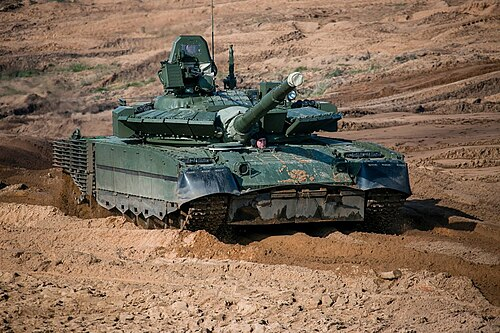
\includegraphics{../images/czolgi/t-80_1.jpg}
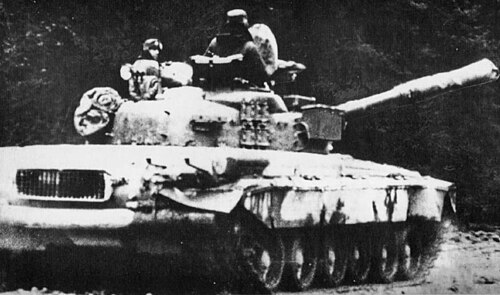
\includegraphics{../images/czolgi/t-80_2.jpg}

\begin{center}\rule{0.5\linewidth}{0.5pt}\end{center}

\subsection{Opis}\label{opis-4}

T-80 to radziecki czołg podstawowy wyposażony w silnik turbinowy ---
jedyny seryjnie produkowany czołg na świecie z takim napędem. Wszedł na
wyposażenie w 1976 roku i był uważany za najbardziej zaawansowany
radziecki czołg swoich czasów. Turbina gazowa GTD-1000 pozwala na
błyskawiczny rozruch nawet w temperaturach -40°C, co czyni T-80
szczególnie wartościowym na teatrze działań w Arktyce i Syberii. Rosja
intensywnie modernizuje T-80 do wersji T-80BVM, wyposażając go w pancerz
reaktywny Relikt, celownik termowizyjny i nowe uzbrojenie.

\subsection{Dane techniczne}\label{dane-techniczne-4}

\begin{longtable}[]{@{}ll@{}}
\toprule\noalign{}
Parametr & Wartość \\
\midrule\noalign{}
\endhead
\bottomrule\noalign{}
\endlastfoot
Typ & Czołg podstawowy \\
Kraj produkcji & ZSRR / Rosja \\
Rok wprowadzenia & 1976 \\
Masa bojowa & 42,5--46 t \\
Długość (z działem) & 9,9 m \\
Szerokość & 3,4 m \\
Wysokość & 2,2 m \\
Uzbrojenie główne & Armata 125 mm 2A46M-4 (gładkolufowa) \\
Uzbrojenie dodatkowe & CKM 7,62 mm PKT, CKM 12,7 mm NSVT \\
Silnik & Turbina gazowa GTD-1000TF, 1 000 KM (T-80BVM: 1 250 KM) \\
Prędkość maks. (droga) & 70--80 km/h \\
Zasięg & 335--500 km \\
Załoga & 3 osoby \\
Pancerz czoła wieży & Kompozytowy + ERA Relikt (T-80BVM) \\
\end{longtable}

\subsection{Charakterystyczne cechy
rozpoznawcze}\label{charakterystyczne-cechy-rozpoznawcze-4}

\begin{quote}
Jak odróżnić T-80 od T-72 i T-90:
\end{quote}

\begin{itemize}
\tightlist
\item
  \textbf{Brak dymu przy ruszaniu:} silnik turbinowy T-80 jest
  praktycznie bezdymny --- w odróżnieniu od diesla T-72/T-90, które przy
  zimnym starcie lub pełnym gazie wydzielają wyraźny dym
\item
  \textbf{Charakterystyczny wizjer kierowcy z przodu kadłuba po lewej:}
  rozmieszczenie przyrządów obserwacyjnych kierowcy jest inne niż w T-72
\item
  \textbf{Pełne koła jezdne z gumową opaską:} T-80 ma koła jezdne bez
  otworów odciążających (pełne), podczas gdy T-72 ma koła z dużymi
  okrągłymi otworami
\item
  \textbf{Wieża o bardziej ostrym, podciętym profilu:} wieża T-80BU/BVM
  jest nieco bardziej kanciastą konstrukcją niż ``grzyb'' T-72
\item
  \textbf{ERA Relikt w wersji BVM:} bloki pancerza reaktywnego Relikt są
  większe i o innym kształcie niż Kontakt-5 na T-72B --- rozmieszczone
  gęściej na czole wieży
\item
  \textbf{Układ wydechowy po lewej stronie kadłuba:} turbina gazowa ma
  charakterystyczny duży okrągły wylot spalin po lewej stronie tylnej
  części kadłuba
\end{itemize}

\subsection{Ciekawostka}\label{ciekawostka-4}

\begin{quote}
T-80 jest jedynym czołgiem, który podczas walk w Groznym w 1994--1995
roku poniósł katastrofalne straty nie z powodu wad konstrukcyjnych, lecz
błędów taktycznych --- wysyłano go bez piechoty wsparcia w wąskie
uliczki miejskie. Paradoksalnie te same czołgi doskonale sprawdziły się
w Syrii, gdzie stosowano je z właściwą taktyką. Turbina gazowa T-80
zużywa przy tym tyle paliwa, że wojsko rosyjskie żartowało, iż czołg
``pije jak samolot''.
\end{quote}

\section{Czołg podstawowy T-90}\label{czoux142g-podstawowy-t-90}

\subsubsection{T-90 Main Battle Tank \textbar{} Т-90 Основной боевой
танк}\label{t-90-main-battle-tank-ux442-90-ux43eux441ux43dux43eux432ux43dux43eux439-ux431ux43eux435ux432ux43eux439-ux442ux430ux43dux43a}

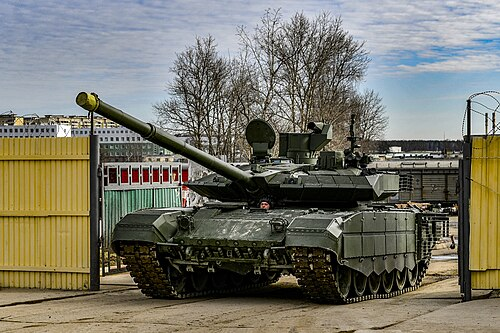
\includegraphics{../images/czolgi/t-90_1.jpg}
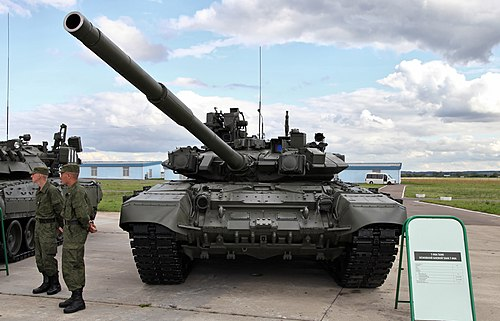
\includegraphics{../images/czolgi/t-90_2.jpg}

\begin{center}\rule{0.5\linewidth}{0.5pt}\end{center}

\subsection{Opis}\label{opis-5}

T-90 to rosyjski czołg podstawowy będący głęboką modernizacją T-72,
wprowadzony do służby w 1992 roku. Stanowi połączenie sprawdzonego
kadłuba T-72 z wieżą i systemem kierowania ogniem zaczerpniętymi z
T-80U. Kluczową cechą wyróżniającą jest system aktywnej ochrony
Sztora-1, który zakłóca systemy naprowadzania przeciwpancernych pocisków
kierowanych. Najnowsza wersja T-90M „Proryw'' wyposażona jest w nową
spawaną wieżę z pancerzem reaktywnym Relikt, celownik Sosna-U z kamerą
termowizyjną i silnik W-92S2F o mocy 1 130 KM. T-90M to aktualnie
najnowocześniejszy seryjnie produkowany czołg rosyjskiej armii.

\subsection{Dane techniczne}\label{dane-techniczne-5}

\begin{longtable}[]{@{}ll@{}}
\toprule\noalign{}
Parametr & Wartość \\
\midrule\noalign{}
\endhead
\bottomrule\noalign{}
\endlastfoot
Typ & Czołg podstawowy \\
Kraj produkcji & Rosja \\
Rok wprowadzenia & 1992 (T-90M: 2020) \\
Masa bojowa & 46,5--48 t \\
Długość (z działem) & 9,53 m \\
Szerokość & 3,78 m \\
Wysokość & 2,22 m \\
Uzbrojenie główne & Armata 125 mm 2A46M-5 \\
Uzbrojenie dodatkowe & CKM 7,62 mm PKT, CKM 12,7 mm Kord \\
Silnik & W-92S2F diesel, 1 130 KM \\
Prędkość maks. (droga) & 65--70 km/h \\
Zasięg & 550--700 km \\
Załoga & 3 osoby \\
System aktywnej ochrony & Sztora-1 (zakłócacz IR) \\
\end{longtable}

\subsection{Charakterystyczne cechy
rozpoznawcze}\label{charakterystyczne-cechy-rozpoznawcze-5}

\begin{quote}
Jak odróżnić T-90 od T-72 i T-80:
\end{quote}

\begin{itemize}
\tightlist
\item
  \textbf{Dwie czerwone ``oczy'' po bokach lufy:} charakterystyczne
  podczerwone reflektory systemu Sztora-1 umieszczone symetrycznie po
  obu stronach lufy --- unikalny element nieobecny w T-72 ani T-80
\item
  \textbf{Nowa spawana wieża T-90M:} wersja M posiada charakterystyczną,
  bardziej kanciastą wieżę z pionowymi ścianami, wyraźnie różniącą się
  od zaokrąglonej wieży T-72 i T-90A
\item
  \textbf{ERA Relikt na całym czole:} bloki pancerza reaktywnego
  pokrywają gęsto czoło kadłuba i wieży, tworząc charakterystyczny
  ``ceglany'' wzór
\item
  \textbf{Termowizja w wieży --- wypukła kopułka po lewej stronie:}
  czujnik termowizyjny celownika Sosna-U to wyraźnie widoczny okrągły
  moduł po lewej stronie wieży
\item
  \textbf{Lufa z rękawem termicznym i wycieraczką:} T-90A/M ma grubą
  czarną osłonę termiczną lufy oraz wycieraczką u nasady --- bardziej
  masywną niż w T-72
\item
  \textbf{Krata przeciwkumulacyjna na tylnej ścianie wieży:} T-90M
  wyposażony jest w charakterystyczną kratownicową osłonę tylnej części
  wieży
\end{itemize}

\subsection{Ciekawostka}\label{ciekawostka-5}

\begin{quote}
W 2016 roku podczas walk w Syrii T-90A przeżył bezpośrednie trafienie
pociskiem TOW-2A --- nagranie zostało opublikowane przez rebeliantów
jako dowód zniszczenia czołgu, tymczasem T-90 odjechał o własnych
siłach. Analiza wykazała, że system Sztora-1 zakłócił laserowe
naprowadzanie pocisku w ostatniej chwili, a pancerz reaktywny pochłonął
większość energii kumulacyjnej. To nagranie stało się niezamierzoną
reklamą rosyjskiego czołgu na całym świecie.
\end{quote}

\section{Niszczyciel czołgów 2S25
Sprut-SD}\label{niszczyciel-czoux142guxf3w-2s25-sprut-sd}

\subsubsection{2S25 Sprut-SD Self-Propelled Anti-Tank Gun \textbar{}
2С25
«Спрут-СД»}\label{s25-sprut-sd-self-propelled-anti-tank-gun-2ux44125-ux441ux43fux440ux443ux442-ux441ux434}

\begin{figure}
\centering
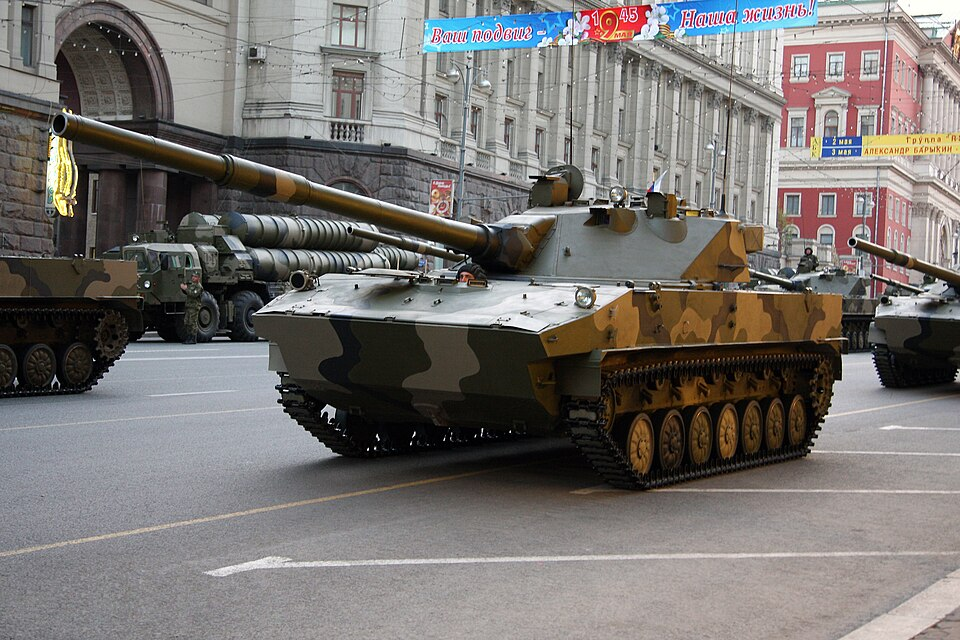
\includegraphics{../images/czolgi/2s25-sprut_1.jpg}
\caption{2S25 Sprut-SD --- widok z boku}
\end{figure}

\begin{center}\rule{0.5\linewidth}{0.5pt}\end{center}

\subsection{Opis}\label{opis-6}

2S25 Sprut-SD (ros. „Ośmiornica'') to rosyjski lekki czołg / samobieżne
działo przeciwpancerne opracowane dla wojsk powietrznodesantowych (WDW).
Weszło do służby w 2005 roku. Przeznaczone do zrzutu na spadochronach
wraz z 3-osobową załogą wewnątrz, jest w pełni amfibijne i może wspinać
się na statki o własnych siłach. Uzbrojone jest w tę samą 125 mm armatę
gładkolufową co T-72, T-80 i T-90 --- przy masie zaledwie 18 ton. W 2010
roku wstrzymano produkcję po pożarze jednego z egzemplarzy podczas
defilady na Placu Czerwonym; w Ukrainie pojawia się od 2022 roku.

\subsection{Dane techniczne}\label{dane-techniczne-6}

\begin{longtable}[]{@{}
  >{\raggedright\arraybackslash}p{(\columnwidth - 2\tabcolsep) * \real{0.5263}}
  >{\raggedright\arraybackslash}p{(\columnwidth - 2\tabcolsep) * \real{0.4737}}@{}}
\toprule\noalign{}
\begin{minipage}[b]{\linewidth}\raggedright
Parametr
\end{minipage} & \begin{minipage}[b]{\linewidth}\raggedright
Wartość
\end{minipage} \\
\midrule\noalign{}
\endhead
\bottomrule\noalign{}
\endlastfoot
Typ & Lekki czołg / niszczyciel czołgów (desantowy) \\
Kraj produkcji & Rosja \\
Rok wprowadzenia & 2005 \\
Masa bojowa & 18 t \\
Długość (z działem) & 9,77 m \\
Silnik & 2V-06-2S diesel, 510 KM \\
Uzbrojenie główne & Armata 125 mm 2A75 (gładkolufowa, z automatem
ładowania) \\
Uzbrojenie dodatkowe & KM 7,62 mm PKT (sprzężony) \\
Prędkość maks. (droga) & 70--71 km/h \\
Prędkość w wodzie & 8--10 km/h \\
Zasięg & 500 km \\
Pancerz & Aluminiowo-kompozytowy; chroni czoło przed 23 mm z 500 m \\
Załoga & 3 osoby (kierowca, działonowy, dowódca) \\
\end{longtable}

\subsection{Charakterystyczne cechy
rozpoznawcze}\label{charakterystyczne-cechy-rozpoznawcze-6}

\begin{quote}
Jak odróżnić 2S25 od BWP i czołgów:
\end{quote}

\begin{itemize}
\tightlist
\item
  \textbf{7 kół nośnych z każdej strony} --- podwozie BMD-3 wydłużono;
  bazowe BMD-3 ma 5 kół; żaden czołg linowy nie wygląda tak ``smukło''
  przy takiej długości
\item
  \textbf{Bardzo niska sylwetka z długą lufą 125 mm bez hamulca
  wylotowego} --- lufa z osłoną termiczną, przedmuchiwaczem pośrodku,
  ale bez charakterystycznego ``kubka'' na końcu
\item
  \textbf{Wieża pośrodku pojazdu} --- dwuosobowa, spawana stalowa wieża
  umieszczona centralnie, nie z tyłu jak w ISU/2S5
\item
  \textbf{Dwa pędniki wodne z tyłu kadłuba} --- widoczne pokrywy
  pędników za ostatnim kołem
\item
  \textbf{Regulowane zawieszenie hydropneumatyczne} --- pojazd może
  ``kucać'' lub ``stawać na palcach'' o 40 cm w górę/dół
\end{itemize}

\subsection{Ciekawostka}\label{ciekawostka-6}

\begin{quote}
2S25 może być zrzucany na spadochronie z Iłami Il-76 z 3-osobową załogą
wewnątrz --- jedyny tak uzbrojony pojazd na świecie zdolny do
samodzielnego wejścia na okręt. W 2010 roku po defiladzie jeden
egzemplarz stanął w płomieniach wskutek wycieku paliwa --- to
wystarczyło by zamknąć linię produkcyjną. Armata 2A75 strzela tą samą
amunicją co T-90, w tym pociskami kierowanymi przez lufę.
\end{quote}

\section{BMD-1 --- bojowy wóz
desantowy}\label{bmd-1-bojowy-wuxf3z-desantowy}

\subsubsection{BMD-1 Airborne Infantry Fighting Vehicle \textbar{}
БМД-1}\label{bmd-1-airborne-infantry-fighting-vehicle-ux431ux43cux434-1}

\begin{figure}
\centering
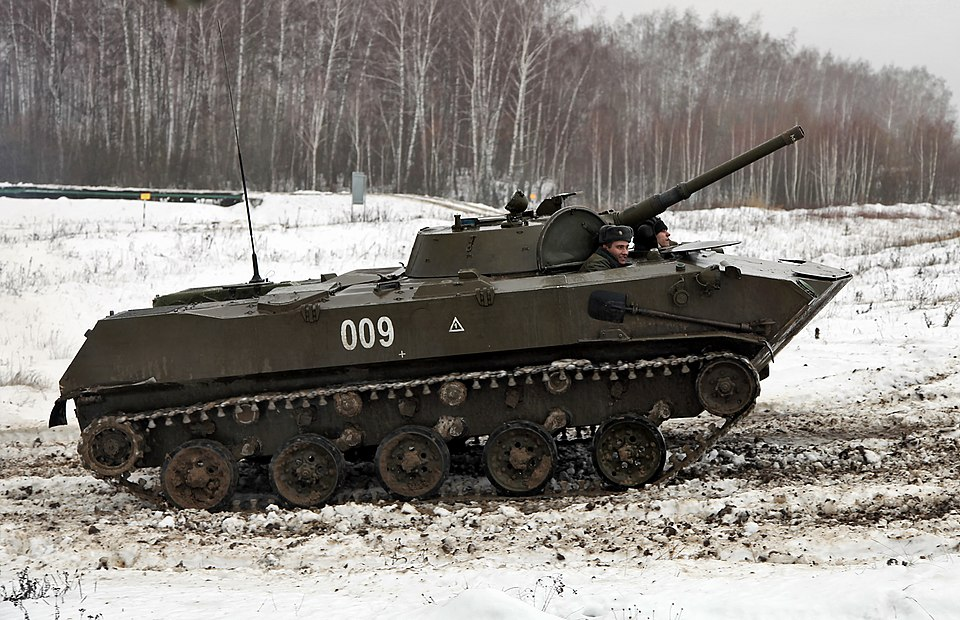
\includegraphics{../images/bwd/bmd-1_1.jpg}
\caption{BMD-1 --- widok z boku}
\end{figure}

\begin{center}\rule{0.5\linewidth}{0.5pt}\end{center}

\subsection{Opis}\label{opis-7}

BMD-1 (Bojewaja Maszyna Diesanta) to radziecki bojowy wóz desantowy,
wprowadzony do służby 14 kwietnia 1969 roku. Zaprojektowany wyłącznie
dla wojsk powietrznodesantowych (WDW) --- może być zrzucany na
spadochronie z samolotu Ił-76 z kierowcą i działonowym siedzącymi
wewnątrz. Uzbrojony w tę samą wieżę co BMP-1, waży jednak zaledwie 8,3 t
--- ponad dwukrotnie mniej. Desant musi wsiadać przez włazy w dachu
(brak tylnych wrót). Używany przez Rosję i Ukrainę od 2014 roku.

\subsection{Dane techniczne}\label{dane-techniczne-7}

\begin{longtable}[]{@{}
  >{\raggedright\arraybackslash}p{(\columnwidth - 2\tabcolsep) * \real{0.5263}}
  >{\raggedright\arraybackslash}p{(\columnwidth - 2\tabcolsep) * \real{0.4737}}@{}}
\toprule\noalign{}
\begin{minipage}[b]{\linewidth}\raggedright
Parametr
\end{minipage} & \begin{minipage}[b]{\linewidth}\raggedright
Wartość
\end{minipage} \\
\midrule\noalign{}
\endhead
\bottomrule\noalign{}
\endlastfoot
Typ & Bojowy wóz desantowy (amfibia) \\
Kraj produkcji & ZSRR \\
Rok wprowadzenia & 1969 \\
Masa bojowa & 8,3 t \\
Długość & 5,41 m \\
Szerokość & 2,53 m \\
Wysokość & 1,97 m \\
Uzbrojenie główne & Armata 73 mm 2A28 Grom (gładkolufowa) \\
Uzbrojenie dodatkowe & PPK 9M14M/9M111M, 3× KM PKT 7,62 mm (w tym 2
kadłubowe) \\
Silnik & 5D-20 diesel, 241--270 KM \\
Prędkość maks. (droga) & 80 km/h \\
Prędkość w wodzie & 10 km/h \\
Zasięg & 600 km \\
Pancerz & Stop aluminium ABT-101; przód kadłuba 15 mm, wieża 6--23 mm \\
Załoga & 2 osoby + 6 desantu \\
\end{longtable}

\subsection{Charakterystyczne cechy
rozpoznawcze}\label{charakterystyczne-cechy-rozpoznawcze-7}

\begin{quote}
Jak odróżnić BMD-1 od BMP-1 i innych wozów:
\end{quote}

\begin{itemize}
\tightlist
\item
  \textbf{Znacznie mniejszy od BMP-1} --- przy identycznej wieży kadłub
  jest wyraźnie krótszy i niższy; BMD-1 wygląda jak ``skurczony BMP-1''
\item
  \textbf{Dwa kadłubowe KM PKT w narożnikach dziobu} --- dwie lufy
  wystające z przednich rogów kadłuba, unikalna cecha nieobecna w BMP
\item
  \textbf{Brak tylnych wrót desantowych} --- desant wsiada wyłącznie
  przez włazy w dachu; tył kadłuba jest zamknięty silnikiem
\item
  \textbf{Regulowane zawieszenie hydropneumatyczne} --- pojazd może się
  ``przykucnąć'' do ok. 100 mm prześwitu lub unieść do 450 mm
\item
  \textbf{Falochron na dziobie} --- składana osłona przeciwfalowa
  unoszona przed wejściem do wody
\item
  \textbf{5 małych kół nośnych równomiernie rozmieszczonych} --- w
  odróżnieniu od 6 kół MT-LB lub nierównomiernego rozstawu T-72
\end{itemize}

\subsection{Ciekawostka}\label{ciekawostka-7}

\begin{quote}
BMD-1 był pierwszym czołgiem/wozem bojowym na świecie zrzucanym na
spadochronie z załogą w środku --- system PRSM-915 z retrorakietami
hamuje opadanie tuż przed lądowaniem. Wcześniej pojazdy zrzucano puste,
a załoga lądowała oddzielnie i często nie mogła znaleźć wozu w terenie.
Identyczna wieża co BMP-1 oznacza, że żołnierze z dystansu mogą pomylić
oba pojazdy --- BMD-1 jest jednak o ponad połowę lżejszy.
\end{quote}

\section{BMD-2 --- bojowy wóz
desantowy}\label{bmd-2-bojowy-wuxf3z-desantowy}

\subsubsection{BMD-2 Airborne Infantry Fighting Vehicle \textbar{}
БМД-2}\label{bmd-2-airborne-infantry-fighting-vehicle-ux431ux43cux434-2}

\begin{figure}
\centering
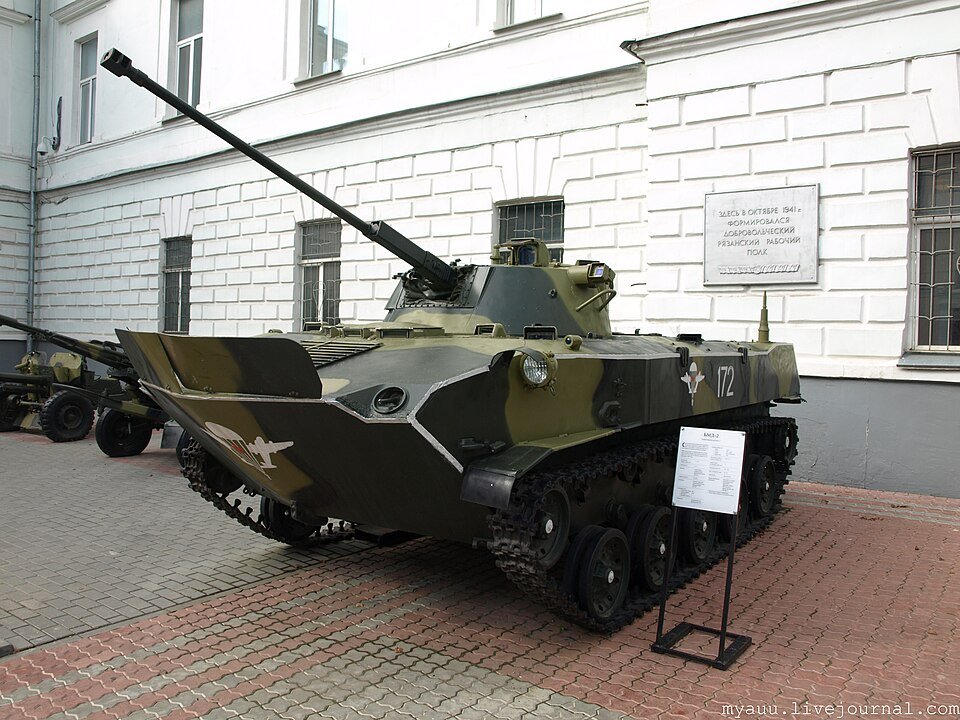
\includegraphics{../images/bwd/bmd-2_1.jpg}
\caption{BMD-2 --- widok z boku}
\end{figure}

\begin{center}\rule{0.5\linewidth}{0.5pt}\end{center}

\subsection{Opis}\label{opis-8}

BMD-2 to radziecka modernizacja BMD-1 wprowadzona do służby w 1985 roku.
Zachowuje kadłub poprzednika, lecz otrzymuje zupełnie nową wieżę B-30 z
działkiem automatycznym 30 mm 2A42 i wyrzutnią PPK --- identyczne
uzbrojenie co BMP-2. Masa wzrosła do 11,5 t. Jak wszystkie BMD, jest w
pełni amfibijny i zrzucany z Iła-76 z załogą w środku. Najliczniej
produkowany wóz rodziny BMD --- jego straty w Ukrainie do 2025 roku
wyniosły ponad 410 egzemplarzy.

\subsection{Dane techniczne}\label{dane-techniczne-8}

\begin{longtable}[]{@{}
  >{\raggedright\arraybackslash}p{(\columnwidth - 2\tabcolsep) * \real{0.5263}}
  >{\raggedright\arraybackslash}p{(\columnwidth - 2\tabcolsep) * \real{0.4737}}@{}}
\toprule\noalign{}
\begin{minipage}[b]{\linewidth}\raggedright
Parametr
\end{minipage} & \begin{minipage}[b]{\linewidth}\raggedright
Wartość
\end{minipage} \\
\midrule\noalign{}
\endhead
\bottomrule\noalign{}
\endlastfoot
Typ & Bojowy wóz desantowy (amfibia) \\
Kraj produkcji & ZSRR \\
Rok wprowadzenia & 1985 \\
Masa bojowa & 11,5 t \\
Długość & 5,91 m (z lufą) / 5,40 m (kadłub) \\
Szerokość & 2,63 m \\
Wysokość & 1,62--1,97 m (regulowane zawieszenie) \\
Uzbrojenie główne & Działko automatyczne 30 mm 2A42 (300 nab.) \\
Uzbrojenie dodatkowe & PPK 9M111 Fagot / 9M113 Konkurs, KM PKT 7,62 mm
(sprzężony), KM PKT 7,62 mm (kadłubowy) \\
Silnik & 5D-20 diesel, 241 KM \\
Prędkość maks. (droga) & 80 km/h \\
Prędkość w wodzie & 10 km/h \\
Zasięg & 450 km \\
Pancerz & Stop aluminium; przód kadłuba 15 mm, wieża 7 mm \\
Załoga & 2 osoby + 6 desantu \\
\end{longtable}

\subsection{Charakterystyczne cechy
rozpoznawcze}\label{charakterystyczne-cechy-rozpoznawcze-8}

\begin{quote}
Jak odróżnić BMD-2 od BMD-1 i BMP-2:
\end{quote}

\begin{itemize}
\tightlist
\item
  \textbf{Długa lufa działka 30 mm zamiast krótkiej armaty 73 mm} ---
  najwyraźniejsza różnica względem BMD-1; lufa 2A42 jest cienka i długa,
  armata Grom w BMD-1 krótka i gruba
\item
  \textbf{Nowa wieża B-30 --- jednoosobowa, mniejsza niż w BMP-2} ---
  specjalnie zaprojektowana dla BMD-2, bo standardowa wieża BMP-2 nie
  mieściła się na małym kadłubie
\item
  \textbf{Wyrzutnia PPK na szczycie wieży} --- sworzniowa wyrzutnia
  Fagot/Konkurs widoczna na górze wieży, zamiast prowadnicy nad działem
  jak w BMD-1
\item
  \textbf{Celownik o dużym kącie uniesienia po lewej stronie lufy} ---
  umożliwia ostrzał celów powietrznych; charakterystyczny element boczny
  wieży
\item
  \textbf{Reflektor z przodu wieży} --- biały reflektor dospawany do
  czoła wieży B-30
\item
  \textbf{Kadłubowy KM w dziobie} --- jak BMD-1, zachowane jedno
  stanowisko PKT z przodu kadłuba (po prawej stronie)
\end{itemize}

\subsection{Ciekawostka}\label{ciekawostka-8}

\begin{quote}
Do 2025 roku Rosja straciła w Ukrainie ponad 410 egzemplarzy BMD-2 ---
więcej niż jakiegokolwiek innego wozu bojowego tego typu. Aluminiowy
pancerz, wystarczający na odłamki, okazał się niemal bezużyteczny wobec
dronów FPV i karabinów maszynowych. BMD-2 to jednocześnie pojazd, który
może wylądować na polu walki w 30 sekund po otwarciu się tylnej rampy
Iła-76 --- z pilotem i działonowym siedzącymi w środku podczas całego
opadania.
\end{quote}

\section{BMD-3 --- bojowy wóz
desantowy}\label{bmd-3-bojowy-wuxf3z-desantowy}

\subsubsection{BMD-3 Airborne Infantry Fighting Vehicle \textbar{}
БМД-3}\label{bmd-3-airborne-infantry-fighting-vehicle-ux431ux43cux434-3}

\begin{figure}
\centering
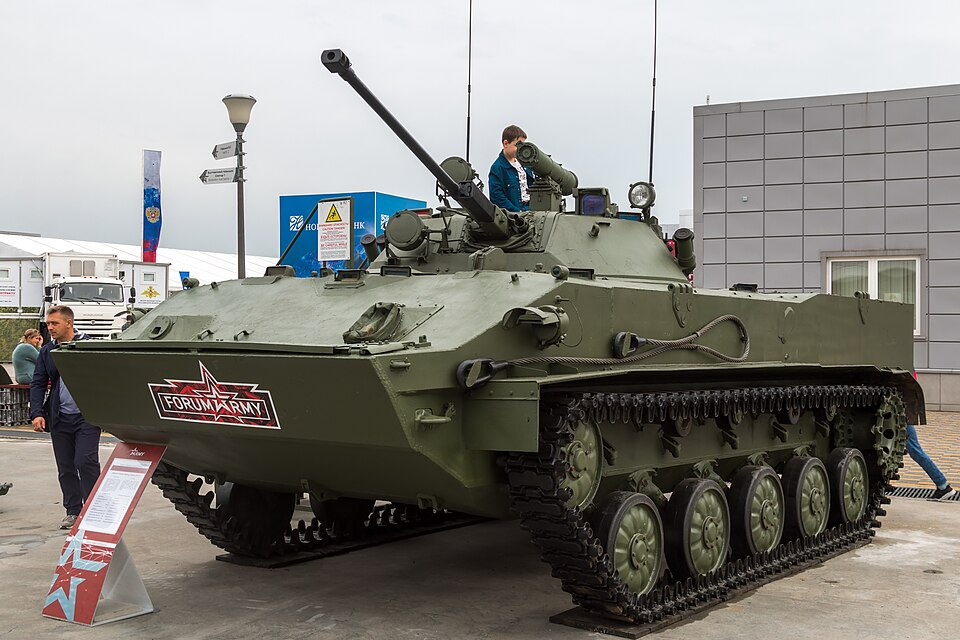
\includegraphics{../images/bwd/bmd-3_1.jpg}
\caption{BMD-3 --- widok z boku}
\end{figure}

\begin{center}\rule{0.5\linewidth}{0.5pt}\end{center}

\subsection{Opis}\label{opis-9}

BMD-3 to radziecki bojowy wóz desantowy trzeciej generacji, przyjęty do
służby w 1990 roku --- ostatni rok ZSRR. W odróżnieniu od BMD-1 i BMD-2
jest całkowicie nową konstrukcją, nie modernizacją. Otrzymał
pełnowymiarową wieżę z BMP-2 oraz unikalne uzbrojenie kadłubowe:
granatnik AGS-17 i karabin RPK-74. Silnik 450 KM i masa 12,9 t.
Wyprodukowano zaledwie 137 egzemplarzy --- z powodu upadku ZSRR
produkcję wstrzymano w 1997 roku. Jego wydłużone podwozie (7 kół)
posłużyło jako baza dla 2S25 Sprut-SD i BTR-MD Rakuszka.

\subsection{Dane techniczne}\label{dane-techniczne-9}

\begin{longtable}[]{@{}
  >{\raggedright\arraybackslash}p{(\columnwidth - 2\tabcolsep) * \real{0.5263}}
  >{\raggedright\arraybackslash}p{(\columnwidth - 2\tabcolsep) * \real{0.4737}}@{}}
\toprule\noalign{}
\begin{minipage}[b]{\linewidth}\raggedright
Parametr
\end{minipage} & \begin{minipage}[b]{\linewidth}\raggedright
Wartość
\end{minipage} \\
\midrule\noalign{}
\endhead
\bottomrule\noalign{}
\endlastfoot
Typ & Bojowy wóz desantowy (amfibia) \\
Kraj produkcji & ZSRR / Rosja \\
Rok wprowadzenia & 1990 \\
Masa bojowa & 12,9 t \\
Długość & 6,00 m \\
Szerokość & 3,13 m \\
Wysokość & 2,25 m \\
Uzbrojenie główne & Działko automatyczne 30 mm 2A42 (500 nab., kąt
podniesienia do 75°) \\
Uzbrojenie dodatkowe & PPK 9M111/9M113, KM PKT 7,62 mm, AGS-17 30 mm
(kadłub lewy), RPK-74 5,45 mm (kadłub prawy) \\
Silnik & 2V-06-2 diesel, 450 KM \\
Prędkość maks. (droga) & 70 km/h \\
Prędkość w wodzie & 10 km/h \\
Zasięg & 500 km \\
Pancerz & Stop aluminium (kadłub) + stal (wieża) \\
Załoga & 3 osoby + 7 desantu (4 przy zrzucie) \\
\end{longtable}

\subsection{Charakterystyczne cechy
rozpoznawcze}\label{charakterystyczne-cechy-rozpoznawcze-9}

\begin{quote}
Jak odróżnić BMD-3 od BMD-1, BMD-2 i BMP-2:
\end{quote}

\begin{itemize}
\tightlist
\item
  \textbf{Pełnowymiarowa wieża BMP-2} --- w odróżnieniu od miniaturowej
  wieży B-30 w BMD-2; identyczna jak w BMP-2, dwuosobowa
\item
  \textbf{Granatnik AGS-17 i karabin RPK-74 w dziobie} --- dwie lufy w
  kadłubie z przodu: AGS-17 po lewej i RPK-74 po prawej; unikalna cecha
  nieobecna w żadnym innym wozie tej rodziny
\item
  \textbf{Wyraźnie większy i szerszy kadłub} --- nowa konstrukcja, nie
  przeróbka BMD-1; szerokość 3,13 m (BMD-2: 2,63 m)
\item
  \textbf{5 kół nośnych w kadłubie bazowym} --- mimo większych rozmiarów
  wersja podstawowa zachowuje 5 kół; 7 kół pojawia się w wydłużonych
  wariantach podwozia (Sprut-SD, Rakuszka)
\item
  \textbf{Wyższy profil niż BMD-2} --- wieża BMP-2 jest wyraźnie wyższa
  niż jednoosobowa B-30
\end{itemize}

\subsection{Ciekawostka}\label{ciekawostka-9}

\begin{quote}
Wyprodukowano tylko 137 egzemplarzy --- tyle co jeden batalion. Upadek
ZSRR w 1991 roku i cięcia budżetowe uniemożliwiły dalszą produkcję. Mimo
to podwozie BMD-3 okazało się na tyle udane, że posłużyło jako baza dla
niszczyciela czołgów 2S25 Sprut-SD (wydłużone do 7 kół) oraz
transportera BTR-MD Rakuszka. Nie odnotowano żadnych strat BMD-3 w
Ukrainie --- prawdopodobnie nie trafiły na front.
\end{quote}

\section{BMD-4 --- bojowy wóz
desantowy}\label{bmd-4-bojowy-wuxf3z-desantowy}

\subsubsection{BMD-4 Airborne Infantry Fighting Vehicle \textbar{}
БМД-4}\label{bmd-4-airborne-infantry-fighting-vehicle-ux431ux43cux434-4}

\begin{figure}
\centering
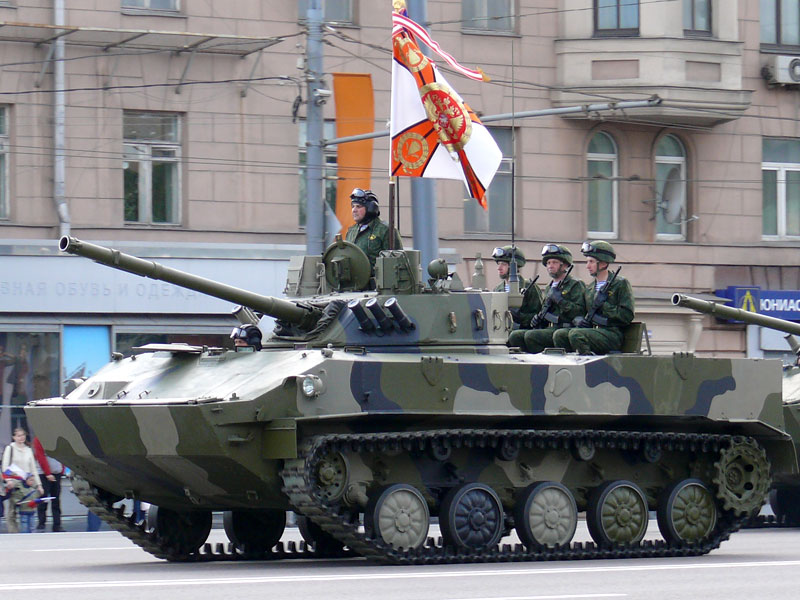
\includegraphics{../images/bwd/bmd-4_1.jpg}
\caption{BMD-4 --- widok z boku}
\end{figure}

\begin{center}\rule{0.5\linewidth}{0.5pt}\end{center}

\subsection{Opis}\label{opis-10}

BMD-4 to rosyjski bojowy wóz desantowy czwartej generacji, przyjęty do
służby 31 grudnia 2004 roku. Kadłub oparty na BMD-3, lecz wyposażony w
zupełnie nowy moduł wieżowy Bachtcha-U łączący armatę 100 mm z działkiem
30 mm --- identyczny zestaw jak w BMP-3. Armata 100 mm może odpalać
laserowo naprowadzane PPK 9M117M1 Arkan przez lufę. Straty Rosji w
Ukrainie: ponad 178 egzemplarzy BMD-4M do marca 2026 roku.

\subsection{Dane techniczne}\label{dane-techniczne-10}

\begin{longtable}[]{@{}
  >{\raggedright\arraybackslash}p{(\columnwidth - 2\tabcolsep) * \real{0.5263}}
  >{\raggedright\arraybackslash}p{(\columnwidth - 2\tabcolsep) * \real{0.4737}}@{}}
\toprule\noalign{}
\begin{minipage}[b]{\linewidth}\raggedright
Parametr
\end{minipage} & \begin{minipage}[b]{\linewidth}\raggedright
Wartość
\end{minipage} \\
\midrule\noalign{}
\endhead
\bottomrule\noalign{}
\endlastfoot
Typ & Bojowy wóz desantowy (amfibia) \\
Kraj produkcji & Rosja \\
Rok wprowadzenia & 2004 \\
Masa bojowa & 13,6 t \\
Długość & 6,36 m (z lufą) / 6,10 m (kadłub) \\
Szerokość & 3,11 m \\
Wysokość & 2,45 m \\
Uzbrojenie główne & Moduł Bachtcha-U: armata 100 mm 2A70 + działko 30 mm
2A72 \\
Amunicja armaty 100 mm & Pociski OFz + PPK 9M117M1 Arkan (przez lufę) \\
Uzbrojenie dodatkowe & KM PKT 7,62 mm, RPK-74 5,45 mm (kadłub prawy),
PPK Fagot/Konkurs (dach wieży) \\
Silnik & 2V-06-2 diesel, 450 KM (BMD-4M: UTD-29, 500 KM) \\
Prędkość maks. (droga) & 70 km/h \\
Prędkość w wodzie & 10 km/h \\
Zasięg & 500 km \\
Pancerz & Stop aluminium (kadłub) + stal (wieża); przód chroni przed 30
mm \\
Załoga & 3 osoby + 5 desantu \\
\end{longtable}

\subsection{Charakterystyczne cechy
rozpoznawcze}\label{charakterystyczne-cechy-rozpoznawcze-10}

\begin{quote}
Jak odróżnić BMD-4 od BMD-3 i BMP-3:
\end{quote}

\begin{itemize}
\tightlist
\item
  \textbf{Dwie sprzężone lufy na wieży: gruba krótka (100 mm) + cienka
  długa (30 mm)} --- unikalna cecha modułu Bachtcha-U; żaden inny wóz
  desantowy nie ma takiego układu
\item
  \textbf{Moduł Bachtcha-U --- niska, zaokrąglona wieża bez wyraźnych
  krawędzi} --- przypomina wieżę BMP-3, ale na mniejszym i węższym
  kadłubie BMD
\item
  \textbf{Wyrzutnia PPK na dachu wieży} --- dodatkowa prowadnica
  Fagot/Konkurs widoczna z tyłu modułu wieżowego
\item
  \textbf{Kadłub identyczny z BMD-3} --- te same proporcje, szerokość
  3,11 m, układ kół; rozpoznawalny po wieży, nie kadłubie
\item
  \textbf{Mniejszy i lżejszy od BMP-3} --- BMD-4 waży 13,6 t, BMP-3 waży
  18,7 t; przy podobnej wieży kadłub jest wyraźnie szczuplejszy
\end{itemize}

\subsection{Ciekawostka}\label{ciekawostka-10}

\begin{quote}
Nazwa modułu Bachtcha-U (Бахча-У) oznacza dosłownie ``melonowe pole''. W
ładowni jednego Iła-76 mieszczą się tylko dwa BMD-4 (wobec trzech
BMD-1/2). Armata 100 mm może odpalać PPK przez lufę --- bez
przeładowania i z pełną osłoną załogi. Do marca 2026 roku Rosja straciła
w Ukrainie 178 wozów BMD-4M, w tym 150 zniszczonych całkowicie.
\end{quote}

\section{Bojowy Wóz Piechoty BMP-1}\label{bojowy-wuxf3z-piechoty-bmp-1}

\subsubsection{BMP-1 Infantry Fighting Vehicle \textbar{} БМП-1 (Боевая
машина
пехоты)}\label{bmp-1-infantry-fighting-vehicle-ux431ux43cux43f-1-ux431ux43eux435ux432ux430ux44f-ux43cux430ux448ux438ux43dux430-ux43fux435ux445ux43eux442ux44b}

\begin{figure}
\centering
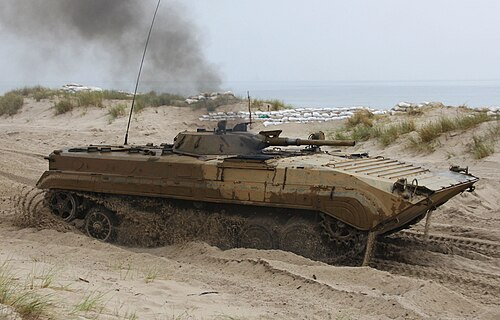
\includegraphics{../images/bwp/bmp-1_1.jpg}
\caption{Zdjęcie 1 - widok z boku}
\end{figure}

\begin{center}\rule{0.5\linewidth}{0.5pt}\end{center}

\subsection{Opis}\label{opis-11}

BMP-1 to radziecki bojowy wóz piechoty, wprowadzony do uzbrojenia w 1966
roku jako pierwszy na świecie seryjnie produkowany pojazd tej klasy ---
łączący zdolność do transportu żołnierzy z rzeczywistą siłą ognia.
Powstał z myślą o wojnie nuklearnej, gdzie piechota musiała prowadzić
działania nie wysiadając z pojazdu, a specjalne strzelnice umożliwiały
żołnierzom desantu ostrzał z wnętrza wozu. Służył i nadal służy w
dziesiątkach armii na całym świecie, a jego bojowy chrzest przeszedł
podczas konfliktu na Bliskim Wschodzie w 1973 roku. Pomimo
przestarzałości uzbrojenia głównego, BMP-1 pozostaje w służbie wielu sił
zbrojnych, w tym armii rosyjskiej, gdzie bywa zastępowany nowszymi
konstrukcjami lub poddawany modernizacji.

\subsection{Dane techniczne}\label{dane-techniczne-11}

\begin{longtable}[]{@{}
  >{\raggedright\arraybackslash}p{(\columnwidth - 2\tabcolsep) * \real{0.5263}}
  >{\raggedright\arraybackslash}p{(\columnwidth - 2\tabcolsep) * \real{0.4737}}@{}}
\toprule\noalign{}
\begin{minipage}[b]{\linewidth}\raggedright
Parametr
\end{minipage} & \begin{minipage}[b]{\linewidth}\raggedright
Wartość
\end{minipage} \\
\midrule\noalign{}
\endhead
\bottomrule\noalign{}
\endlastfoot
Typ & Bojowy wóz piechoty \\
Kraj produkcji & ZSRR \\
Rok wprowadzenia & 1966 \\
Masa bojowa & 13,2 t \\
Długość & 6,74 m \\
Szerokość & 2,94 m \\
Wysokość & 2,07 m \\
Uzbrojenie główne & Armata gładkolufowa 73 mm 2A28 Grom + wyrzutnia PPKR
9M14 Malyutka \\
Uzbrojenie dodatkowe & km 7,62 mm PKT (sprzężony) \\
Silnik & UTD-20 V6 diesel \\
Moc silnika & 300 KM \\
Prędkość maks. (droga) & 65 km/h \\
Prędkość na wodzie & 7--8 km/h \\
Zasięg & 600 km \\
Załoga + desant & 3 + 8 os. \\
\end{longtable}

\subsection{Charakterystyczne cechy
rozpoznawcze}\label{charakterystyczne-cechy-rozpoznawcze-11}

\begin{quote}
Jak odróżnić BMP-1 od innych podobnych modeli:
\end{quote}

\begin{itemize}
\tightlist
\item
  \textbf{Wieżyczka stożkowa, niska i okrągła:} Charakterystyczna mała
  wieżyczka o stożkowym kształcie, wyraźnie niższa niż w BMP-2 i BMP-3
  --- oglądana z boku przypomina ścięty stożek.
\item
  \textbf{Działo 73 mm z wyraźnym tłumikiem płomieni:} Gruba, krótka
  lufa z wydatnym, cylindrycznym tłumikiem płomieni na końcu ---
  zupełnie inny wygląd niż smukła lufa 30 mm autocannon w BMP-2.
\item
  \textbf{Wyrzutnia rakiet PPKR na wieżyczce:} Ponad lufą armaty
  widoczna jest szyna wyrzutni rakiet przeciwpancernych Malyutka ---
  charakterystyczny element górnej sylwetki.
\item
  \textbf{Nisko położony, pochyły dziób kadłuba:} Przednia część kadłuba
  jest bardzo stromo pochylona, z charakterystycznymi podłużnymi żebrami
  wzmacniającymi --- tworzy ostry, klinkowy kształt z przodu.
\item
  \textbf{Prostokątne włazy desantu na rufie:} Z tyłu wozu widoczne są
  duże, prostokątne drzwi tylne (służą jednocześnie jako zbiorniki
  paliwa) otwierane na zewnątrz --- charakterystyczna cecha odróżniająca
  od BMP-3.
\item
  \textbf{Porty strzeleckie wzdłuż burt:} Wzdłuż bocznych powierzchni
  kadłuba widoczne są charakterystyczne małe, owalne otwory strzelnicze
  dla żołnierzy desantu --- wyraźnie widoczne w liczbie 4 po każdej
  stronie.
\end{itemize}

\subsection{Ciekawostka}\label{ciekawostka-11}

\begin{quote}
BMP-1 był tak nowatorski w chwili powstania, że NATO przez długi czas
nie potrafiło właściwie ocenić jego możliwości bojowych --- zachodnie
wywiady sądziły, że ta mała maszyna nie może jednocześnie być amfibią,
przewozić ośmiu żołnierzy i posiadać tak silnego uzbrojenia. Dopiero
zdobyte egzemplarze z wojen na Bliskim Wschodzie pozwoliły Zachodowi
zrozumieć rewolucję, jaką BMP-1 wprowadził na pole walki.
\end{quote}

\section{Bojowy Wóz Piechoty BMP-2}\label{bojowy-wuxf3z-piechoty-bmp-2}

\subsubsection{BMP-2 Infantry Fighting Vehicle \textbar{} БМП-2 (Боевая
машина
пехоты)}\label{bmp-2-infantry-fighting-vehicle-ux431ux43cux43f-2-ux431ux43eux435ux432ux430ux44f-ux43cux430ux448ux438ux43dux430-ux43fux435ux445ux43eux442ux44b}

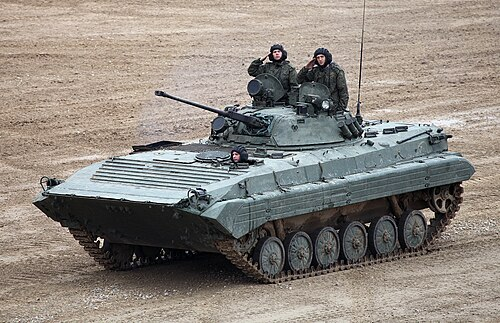
\includegraphics{../images/bwp/bmp-2_1.jpg}
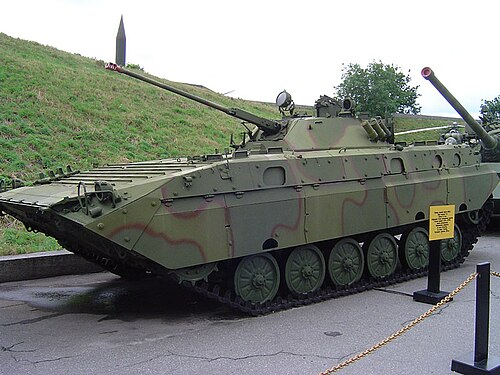
\includegraphics{../images/bwp/bmp-2_2.jpg}

\begin{center}\rule{0.5\linewidth}{0.5pt}\end{center}

\subsection{Opis}\label{opis-12}

BMP-2 to radziecka modernizacja BMP-1, wprowadzona do uzbrojenia w 1980
roku jako bezpośrednia odpowiedź na doświadczenia bojowe --- przede
wszystkim słabość 73 mm armaty BMP-1 w walce z lotnictwem i słabo
opancerzonymi pojazdami. Kluczową zmianą było zastąpienie stożkowej
jednoosobowej wieżyczki nową, dwuosobową wieżą uzbrojoną w
szybkostrzelną armatę automatyczną 30 mm 2A42, zdolną razić zarówno
pojazdy opancerzone, jak i cele powietrzne. BMP-2 przeszedł chrzest
bojowy w Afganistanie, gdzie jego armata 30 mm okazała się o wiele
skuteczniejsza w walce w górach niż uzbrojenie poprzednika. Do dziś
BMP-2 pozostaje podstawowym BWP armii rosyjskiej i jest eksploatowany w
ponad 30 krajach świata.

\subsection{Dane techniczne}\label{dane-techniczne-12}

\begin{longtable}[]{@{}
  >{\raggedright\arraybackslash}p{(\columnwidth - 2\tabcolsep) * \real{0.5263}}
  >{\raggedright\arraybackslash}p{(\columnwidth - 2\tabcolsep) * \real{0.4737}}@{}}
\toprule\noalign{}
\begin{minipage}[b]{\linewidth}\raggedright
Parametr
\end{minipage} & \begin{minipage}[b]{\linewidth}\raggedright
Wartość
\end{minipage} \\
\midrule\noalign{}
\endhead
\bottomrule\noalign{}
\endlastfoot
Typ & Bojowy wóz piechoty \\
Kraj produkcji & ZSRR / Rosja \\
Rok wprowadzenia & 1980 \\
Masa bojowa & 14,3 t \\
Długość & 6,74 m \\
Szerokość & 3,15 m \\
Wysokość & 2,45 m \\
Uzbrojenie główne & Armata automatyczna 30 mm 2A42 + wyrzutnia PPKR
9P135M (Fagot/Konkurs) \\
Uzbrojenie dodatkowe & km 7,62 mm PKT (sprzężony) \\
Silnik & UTD-20/3 diesel \\
Moc silnika & 300 KM \\
Prędkość maks. (droga) & 65 km/h \\
Prędkość na wodzie & 7 km/h \\
Zasięg & 600 km \\
Załoga + desant & 3 + 7 os. \\
\end{longtable}

\subsection{Charakterystyczne cechy
rozpoznawcze}\label{charakterystyczne-cechy-rozpoznawcze-12}

\begin{quote}
Jak odróżnić BMP-2 od innych podobnych modeli:
\end{quote}

\begin{itemize}
\tightlist
\item
  \textbf{Dwuosobowa, wyraźnie wyższa wieżyczka:} Wieża BMP-2 jest
  wyraźnie wyższa i bardziej masywna niż stożkowa wieżyczka BMP-1,
  mieści dwóch ludzi (dowódcę i działonowego) --- jest to najbardziej
  rzucająca się w oczy różnica.
\item
  \textbf{Smukła, długa lufa armaty 30 mm:} Cienka, długa lufa
  autocannonu 2A42 z charakterystycznym cylindrycznym tłumikiem płomieni
  --- znacznie smuklejsza i dłuższa niż grube działo BMP-1.
\item
  \textbf{Wyrzutnia PPKR po lewej stronie wieży:} Na lewym boku wieży
  widoczna jest szyna z wyrzutnią rakiet przeciwpancernych (Fagot lub
  Konkurs) --- umieszczona z boku, nie nad lufą jak w BMP-1.
\item
  \textbf{Wyraźne pochylenie lufy ku górze:} Armata 2A42 może być
  unoszona pod znacznym kątem elewacji (do +74°), dzięki czemu BMP-2 w
  gotowości bojowej często prezentuje lufę uniesioną bardziej ku górze
  niż BMP-1.
\item
  \textbf{Kadłub identyczny z BMP-1:} Dolna część wozu --- kadłub, układ
  jezdny, tylne drzwi --- jest praktycznie taka sama jak w BMP-1. Jeśli
  wieżyczka jest nowa, a kadłub wygląda jak BMP-1, to jest BMP-2.
\item
  \textbf{Strzelnice desantowe --- mniej niż w BMP-1:} BMP-2 ma mniejszą
  liczbę strzelnic bocznych (mniej żołnierzy desantu: 7 zamiast 8), ale
  są one podobnego kształtu jak w poprzedniku.
\end{itemize}

\subsection{Ciekawostka}\label{ciekawostka-12}

\begin{quote}
Armata 2A42 zastosowana w BMP-2 ma aż dwa podajniki amunicji, co pozwala
działonowemu przełączać w locie między amunicją przeciwpancerną a
odłamkowo-burzącą --- bez konieczności zatrzymywania się czy
przeładowania. To rozwiązanie, niespotykane w ówczesnych zachodnich
pojazdach, dawało rosyjskim żołnierzom ogromną elastyczność w walce z
różnymi celami.
\end{quote}

\section{Bojowy Wóz Piechoty BMP-3}\label{bojowy-wuxf3z-piechoty-bmp-3}

\subsubsection{BMP-3 Infantry Fighting Vehicle \textbar{} БМП-3 (Боевая
машина
пехоты)}\label{bmp-3-infantry-fighting-vehicle-ux431ux43cux43f-3-ux431ux43eux435ux432ux430ux44f-ux43cux430ux448ux438ux43dux430-ux43fux435ux445ux43eux442ux44b}

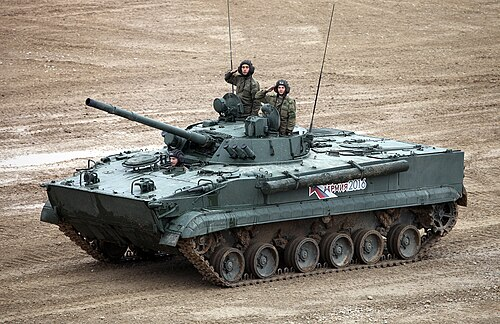
\includegraphics{../images/bwp/bmp-3_1.jpg}
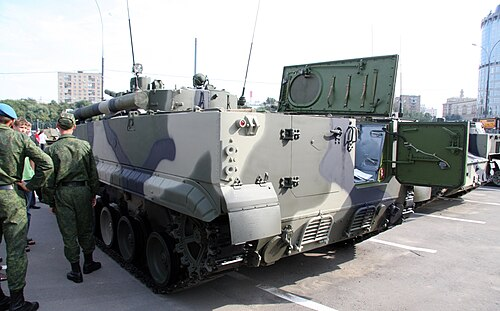
\includegraphics{../images/bwp/bmp-3_2.jpg}

\begin{center}\rule{0.5\linewidth}{0.5pt}\end{center}

\subsection{Opis}\label{opis-13}

BMP-3 to rosyjski bojowy wóz piechoty trzeciej generacji, wprowadzony do
służby w 1987 roku, zaprojektowany jako całkowicie nowa konstrukcja ---
nie ewolucja, lecz rewolucja w stosunku do BMP-1 i BMP-2. Jego unikalną
cechą jest wyjątkowo silne uzbrojenie: kombinacja niskociśnieniowej
armaty 100 mm (zdolnej też do odpalania rakiet ppanc.), szybkostrzelnego
autocannonu 30 mm i trzech karabinów maszynowych 7,62 mm czyni z niego
wóz o ogniowej sile porównywalnej z niektórymi czołgami lekkimi. BMP-3
jest dziś podstawowym BWP armii rosyjskiej i uczestniczy w walkach na
Ukrainie od 2022 roku; eksportowany był m.in. do Emiratów Arabskich,
Kuwejtu i Korei Południowej. Jego złożoność i wyższy koszt produkcji
sprawił, że nigdy nie zastąpił w pełni BMP-2 w Siłach Zbrojnych
Federacji Rosyjskiej.

\subsection{Dane techniczne}\label{dane-techniczne-13}

\begin{longtable}[]{@{}
  >{\raggedright\arraybackslash}p{(\columnwidth - 2\tabcolsep) * \real{0.5263}}
  >{\raggedright\arraybackslash}p{(\columnwidth - 2\tabcolsep) * \real{0.4737}}@{}}
\toprule\noalign{}
\begin{minipage}[b]{\linewidth}\raggedright
Parametr
\end{minipage} & \begin{minipage}[b]{\linewidth}\raggedright
Wartość
\end{minipage} \\
\midrule\noalign{}
\endhead
\bottomrule\noalign{}
\endlastfoot
Typ & Bojowy wóz piechoty \\
Kraj produkcji & ZSRR / Rosja \\
Rok wprowadzenia & 1987 \\
Masa bojowa & 18,7 t \\
Długość & 7,14 m \\
Szerokość & 3,20 m \\
Wysokość & 2,40 m \\
Uzbrojenie główne & Armata 100 mm 2A70 + autocannon 30 mm 2A72 + PPKR
9M117 Bastion \\
Uzbrojenie dodatkowe & 3 × km 7,62 mm PKT \\
Silnik & UTD-29M diesel \\
Moc silnika & 500 KM \\
Prędkość maks. (droga) & 72 km/h \\
Prędkość na wodzie & 10 km/h \\
Zasięg & 600 km \\
Załoga + desant & 3 + 7 os. \\
\end{longtable}

\subsection{Charakterystyczne cechy
rozpoznawcze}\label{charakterystyczne-cechy-rozpoznawcze-13}

\begin{quote}
Jak odróżnić BMP-3 od innych podobnych modeli:
\end{quote}

\begin{itemize}
\tightlist
\item
  \textbf{Duża, dwuosobowa wieża z dwiema lufami:} Najbardziej
  charakterystyczna cecha --- wieża BMP-3 nosi dwie lufy obok siebie:
  grubą, krótką armatę 100 mm po lewej i smukły autocannon 30 mm po
  prawej stronie. Żaden inny BWP nie ma takiej konfiguracji.
\item
  \textbf{Masywna, zaokrąglona wieża o dużej średnicy podstawy:} Wieża
  BMP-3 jest wyraźnie większa i bardziej zaokrąglona niż wieże BMP-1 i
  BMP-2 --- zajmuje znaczną część górnej powierzchni kadłuba.
\item
  \textbf{Silnik z tyłu, kierowca w centrum kadłuba:} W odróżnieniu od
  BMP-1 i BMP-2 (silnik z przodu), BMP-3 ma silnik z tyłu --- kierowca
  siedzi centralnie w przedziale desantowym, co widać po centralnym
  włazie kierowcy na dziobie kadłuba.
\item
  \textbf{Trzy włazy desantowe na rufie i właz kierowcy z przodu:}
  Żołnierze desantu opuszczają pojazd przez otwory w tylnym pancerzu
  (dwa mniejsze boczne klapy i jeden centralny), a nie przez duże tylne
  drzwi jak w BMP-1/2.
\item
  \textbf{Wyraźnie szerszy i dłuższy kadłub:} BMP-3 jest widocznie
  większy od poprzedników: dłuższy (7,14 vs 6,74 m) i wyraźnie cięższy
  (18,7 t vs 13--14 t) --- sprawia wrażenie masywniejszego, pełniejszego
  w kształcie pojazdu.
\item
  \textbf{Specjalne wywietrzniki silnika z tyłu kadłuba:} Na tylnej
  ścianie kadłuba BMP-3 widoczne są duże kratki wentylacyjne silnika
  umieszczonego z tyłu --- w BMP-1/2 tylna ściana to przede wszystkim
  drzwi desantowe.
\end{itemize}

\subsection{Ciekawostka}\label{ciekawostka-13}

\begin{quote}
BMP-3 może strzelać rakietami przeciwpancernymi bezpośrednio przez lufę
armaty 100 mm --- technologia zwana ATGM-through-the-barrel pozwala na
precyzyjne rażenie celów opancerzonych na odległość do 4 km, przy czym
pojazd nie musi zatrzymywać się ani odsłaniać wyrzutni ponad pancerzem.
Czyni to z niego jeden z nielicznych BWP zdolnych do skutecznej walki z
czołgami na dużych dystansach bez narażania załogi.
\end{quote}

\section{MT-LB --- wielozadaniowy transporter
opancerzony}\label{mt-lb-wielozadaniowy-transporter-opancerzony}

\subsubsection{MT-LB Armored Personnel Carrier / Artillery Tractor
\textbar{}
МТ-ЛБ}\label{mt-lb-armored-personnel-carrier-artillery-tractor-ux43cux442-ux43bux431}

\begin{figure}
\centering
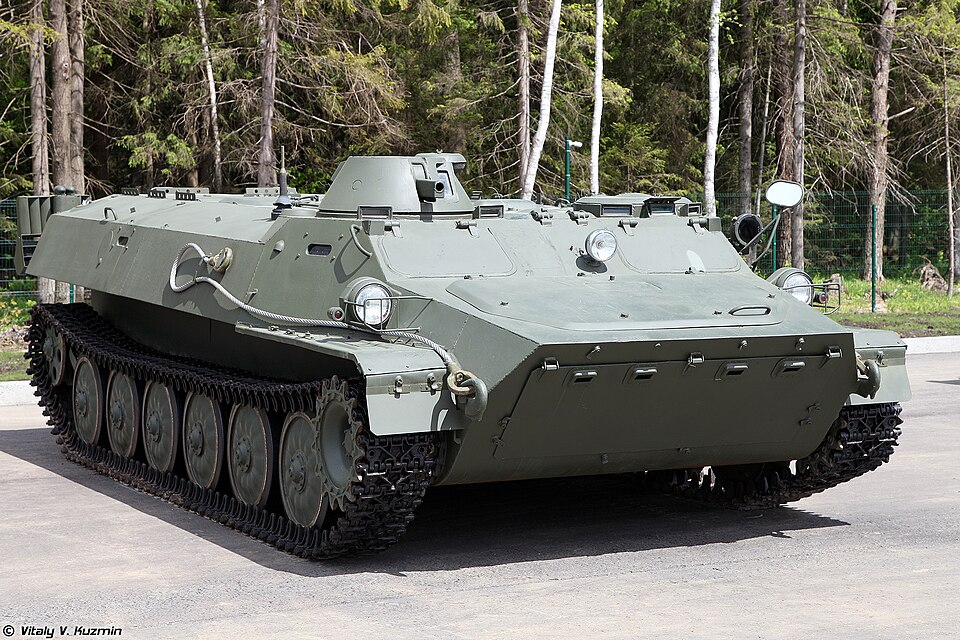
\includegraphics{../images/apc/mt-lb_1.jpg}
\caption{MT-LB --- widok z boku}
\end{figure}

\begin{center}\rule{0.5\linewidth}{0.5pt}\end{center}

\subsection{Opis}\label{opis-14}

MT-LB (Mnogotselevoy Tyagach Legky Bronirovany --- lekki opancerzony
ciągnik wielozadaniowy) to radziecki amfibijny transporter opancerzony i
ciągnik artyleryjski wprowadzony w latach 70. XX wieku. Zaprojektowany
na bazie komercyjnych podzespołów samochodów ciężarowych, jest wyjątkowo
tani i niezawodny. Może przewozić 11 żołnierzy lub 2000 kg ładunku,
holować działa do 6500 kg. Stał się bazą dla dziesiątek wariantów: 2S1
Goździk, Strela-10, radarów SNAR, niszczycieli czołgów. Rosja straciła w
Ukrainie ponad 1710 egzemplarzy --- więcej niż jakiegokolwiek innego
pojazdu.

\subsection{Dane techniczne}\label{dane-techniczne-14}

\begin{longtable}[]{@{}ll@{}}
\toprule\noalign{}
Parametr & Wartość \\
\midrule\noalign{}
\endhead
\bottomrule\noalign{}
\endlastfoot
Typ & Transporter opancerzony / ciągnik artyleryjski (amfibia) \\
Kraj produkcji & ZSRR \\
Rok wprowadzenia & ok. 1970 \\
Masa bojowa & 11,9 t \\
Długość & 6,45 m \\
Szerokość & 2,86 m \\
Wysokość & 1,86 m \\
Uzbrojenie & KM PKT 7,62 mm w małej wieżyczce \\
Ładowność & 11 żołnierzy lub 2000 kg ładunku \\
Siła ciągu & holowanie do 6500 kg \\
Silnik & YaMZ-238 diesel, 240 KM \\
Prędkość maks. (droga) & 61 km/h \\
Prędkość w wodzie & 5--6 km/h (napęd gąsienicami) \\
Zasięg & 500 km \\
Pancerz & Stal 3--14 mm (ochrona przed bronią strzelecką i odłamkami) \\
Załoga & 2 osoby + 11 desantu \\
\end{longtable}

\subsection{Charakterystyczne cechy
rozpoznawcze}\label{charakterystyczne-cechy-rozpoznawcze-14}

\begin{quote}
Jak odróżnić MT-LB od BTR-80 i BMP:
\end{quote}

\begin{itemize}
\tightlist
\item
  \textbf{Mała wieżyczka z PKT przesunięta ku przodowi po prawej
  stronie} --- niska, jednoosobowa kopułka; brak większej wieży; wygląda
  jak ``transporter bez wieży z guzkiem z boku''
\item
  \textbf{Bardzo niska i płaska sylwetka} --- wysokość tylko 1,86 m;
  znacznie niższy niż BTR-80 (2,35 m) i BMP-2 (2,06 m)
\item
  \textbf{Sześć kół nośnych równomiernie rozmieszczonych} --- widoczne z
  boku; wariant MT-LBu ma 7 kół i wyższy kadłub
\item
  \textbf{Napęd w wodzie gąsienicami} (bez śrub) --- podczas pływania
  nie widać wychylanych napędników; porusza się wolno i niezgrabnie na
  wodzie
\item
  \textbf{Szerokie gąsienice w wersji MT-LBV} --- zimowa odmiana ma
  gąsienice 670 mm (vs 350 mm w standardzie); wygląda jak
  ``rozkroczony'' transporter
\item
  \textbf{Często z doposażeniem na dachu} --- w Ukrainie powszechnie
  montowane: ZU-23-2, S-60, wieże BMP, wyrzutnie rakiet --- każda
  kombinacja jest inna
\end{itemize}

\subsection{Warianty na bazie MT-LB}\label{warianty-na-bazie-mt-lb}

\begin{longtable}[]{@{}
  >{\raggedright\arraybackslash}p{(\columnwidth - 2\tabcolsep) * \real{0.6000}}
  >{\raggedright\arraybackslash}p{(\columnwidth - 2\tabcolsep) * \real{0.4000}}@{}}
\toprule\noalign{}
\begin{minipage}[b]{\linewidth}\raggedright
Wariant
\end{minipage} & \begin{minipage}[b]{\linewidth}\raggedright
Opis
\end{minipage} \\
\midrule\noalign{}
\endhead
\bottomrule\noalign{}
\endlastfoot
MT-LBu & Wydłużony kadłub (7 kół), mocniejszy silnik --- baza dla 2S1,
Strela-10, SNAR \\
MT-LBV & Szersze gąsienice (670 mm) do działania na śniegu i bagnach \\
MT-LBM 6MB & Moduł z działkiem 30 mm na dachu \\
2S1 Goździk & Haubica 122 mm na podwoziu MT-LBu \\
9P149 Shturm-S & Niszczyciel czołgów z PPK Szturm na podwoziu MT-LBu \\
Strela-10 & Zestaw rakietowy plot. na podwoziu MT-LBu \\
\end{longtable}

\subsection{Ciekawostka}\label{ciekawostka-14}

\begin{quote}
MT-LB zbudowano z części samochodów ciężarowych --- silnik V8 pochodzi
wprost z cywilnych ciężarówek. To sprawiło, że był ekstremalnie tani i
produkowany w ogromnych ilościach. W Ukrainie Rosjanie w desperacji
montowali na MT-LB nie tylko ZU-23-2 i S-60, ale nawet okrętowe
wyrzutnie bomb głębinowych RBU-6000. Ukraina posiadała przed wojną ponad
2090 sztuk --- Rosja straciła ich ponad 1710, co czyni MT-LB najbardziej
stratnym pojazdem konfliktu.
\end{quote}

\section{Transporter Opancerzony
BTR-80}\label{transporter-opancerzony-btr-80}

\subsubsection{BTR-80 Armoured Personnel Carrier \textbar{}
Бронетранспортёр
БТР-80}\label{btr-80-armoured-personnel-carrier-ux431ux440ux43eux43dux435ux442ux440ux430ux43dux441ux43fux43eux440ux442ux451ux440-ux431ux442ux440-80}

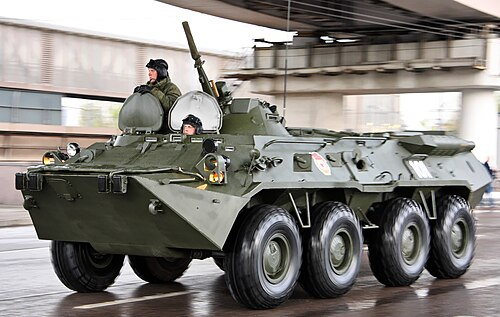
\includegraphics{../images/apc/btr-80_1.jpg}
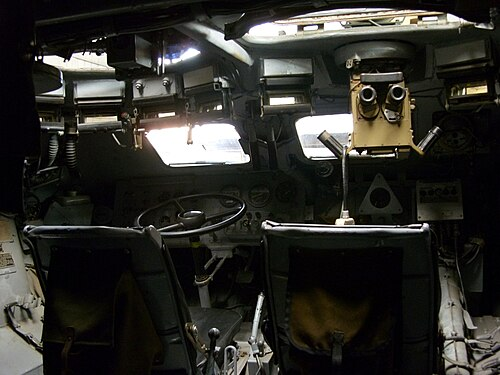
\includegraphics{../images/apc/btr-80_2.jpg}

\begin{center}\rule{0.5\linewidth}{0.5pt}\end{center}

\subsection{Opis}\label{opis-15}

BTR-80 (ros. Бронетранспортёр-80) to ośmiokołowy kołowy transporter
opancerzony produkcji radzieckiej, przyjęty na uzbrojenie Armii
Radzieckiej w 1985 roku jako następca starszych BTR-60 i BTR-70.
Zaprojektowany z myślą o przewożeniu piechoty zmotoryzowanej na polu
walki i zapewnieniu jej bezpośredniego wsparcia ogniowego, jest zdolny
do pływania na wodzie. To jeden z najliczniej produkowanych i
eksportowanych transporterów opancerzonych na świecie --- służy w ponad
40 armiach. Wojsko rosyjskie używa go masowo do dziś, choć w Ukrainie
pojazdy te poniosły bardzo duże straty.

\subsection{Dane techniczne}\label{dane-techniczne-15}

\begin{longtable}[]{@{}
  >{\raggedright\arraybackslash}p{(\columnwidth - 2\tabcolsep) * \real{0.5263}}
  >{\raggedright\arraybackslash}p{(\columnwidth - 2\tabcolsep) * \real{0.4737}}@{}}
\toprule\noalign{}
\begin{minipage}[b]{\linewidth}\raggedright
Parametr
\end{minipage} & \begin{minipage}[b]{\linewidth}\raggedright
Wartość
\end{minipage} \\
\midrule\noalign{}
\endhead
\bottomrule\noalign{}
\endlastfoot
Typ & Transporter opancerzony kołowy \\
Kraj produkcji & ZSRR / Rosja \\
Rok wprowadzenia & 1985 \\
Masa bojowa & 13,6 t \\
Długość & 7,7 m \\
Szerokość & 2,9 m \\
Wysokość & 2,41 m \\
Uzbrojenie & 14,5 mm KPVT + 7,62 mm PKT (wieżyczka NSVT); wariant
BTR-80A: 30 mm armata 2A72 \\
Silnik & KamAZ-7403 (turbodiesel) \\
Moc silnika & 260 KM \\
Prędkość maks. (droga) & 80--90 km/h \\
Prędkość na wodzie & 10 km/h \\
Zasięg & 600 km \\
Załoga + desant & 3 + 7 os. \\
Napęd & Kołowy 8×8, amfibijny \\
\end{longtable}

\subsection{Charakterystyczne cechy
rozpoznawcze}\label{charakterystyczne-cechy-rozpoznawcze-15}

\begin{quote}
Jak odróżnić BTR-80 od innych podobnych pojazdów:
\end{quote}

\begin{itemize}
\tightlist
\item
  \textbf{Kształt kadłuba --- pochylony dziób:} Przednia część kadłuba
  jest wyraźnie pochylona pod kątem ok. 60°, z charakterystycznym
  zaokrąglonym ``nosem'' --- bardziej zaokrąglonym niż w BTR-60/70,
  mniej kanciaste niż w BTR-90.
\item
  \textbf{Mała okrągła wieżyczka z podwójnym uzbrojeniem:} Standardowy
  BTR-80 ma małą, otwartą wieżyczkę z karabinem maszynowym 14,5 mm KPVT
  i 7,62 mm PKT umieszczonym obok (nie w osi); BTR-80A ma zamkniętą
  wieżyczkę z armatą 30 mm.
\item
  \textbf{Osiem dużych kół bez gąsienic:} Cztery osie z kołami o dużej
  średnicy --- wyraźnie widoczne przestrzenie między kołami 1.--2. a
  3.--4. osią.
\item
  \textbf{Drzwi boczne z przegubem pośrodku pojazdu:} Charakterystyczne
  drzwi dzielone (górna i dolna część otwierają się osobno) znajdują się
  w środkowej części kadłuba między 2. a 3. osią --- żołnierze wysiadają
  na zewnątrz, a nie przez tył.
\item
  \textbf{Niska sylwetka w stosunku do szerokości:} Pojazd jest
  stosunkowo niski (2,41 m) i szeroki, co daje mu charakterystyczny
  ``płaski'' profil w porównaniu z BTR-90 czy Tajfunem.
\item
  \textbf{Brak tylnej rampy desantowej:} W odróżnieniu od BWP-1/2 i
  wielu zachodnich APC, BTR-80 nie ma tylnej rampy --- desant wysiada
  przez drzwi boczne, co jest jego wyraźną słabością rozpoznawaną przez
  obserwatorów.
\end{itemize}

\subsection{Ciekawostka}\label{ciekawostka-15}

\begin{quote}
BTR-80 ma jeden silnik (KamAZ-7403 diesel), co było ogromnym krokiem
naprzód w stosunku do poprzednika BTR-70, który miał dwa silniki
benzynowe GAZ-49B --- mechanicy BTR-70 musieli obsługiwać dwa odrębne
układy napędowe, co znacznie komplikowało eksploatację i serwisowanie w
warunkach polowych.
\end{quote}

\section{Transporter Opancerzony
BTR-90}\label{transporter-opancerzony-btr-90}

\subsubsection{BTR-90 Armoured Personnel Carrier \textbar{}
Бронетранспортёр
БТР-90}\label{btr-90-armoured-personnel-carrier-ux431ux440ux43eux43dux435ux442ux440ux430ux43dux441ux43fux43eux440ux442ux451ux440-ux431ux442ux440-90}

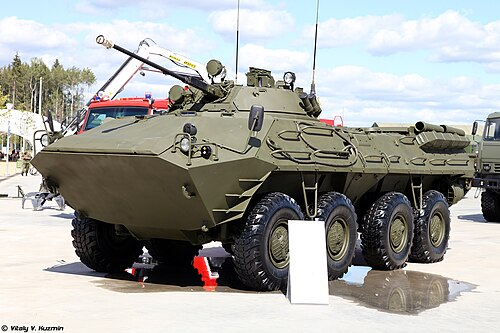
\includegraphics{../images/apc/btr-90_1.jpg}
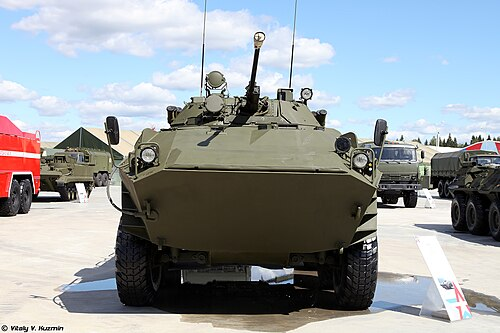
\includegraphics{../images/apc/btr-90_2.jpg}

\begin{center}\rule{0.5\linewidth}{0.5pt}\end{center}

\subsection{Opis}\label{opis-16}

BTR-90 (ros. Бронетранспортёр-90, znany też jako ``Rostok'') to rosyjski
ośmiokołowy amfibijny transporter opancerzony opracowany w latach 90. XX
wieku jako zaawansowany następca BTR-80. Pojazd jest wyraźnie większy i
cięższy od poprzednika, a jego główną cechą wyróżniającą jest wieżyczka
identyczna jak w BWP-2 --- z automatyczną armatą 30 mm 2A42, co daje mu
znacznie większą siłę ognia niż typowy APC. Mimo obiecujących
parametrów, Rosja ostatecznie zrezygnowała z zakupu BTR-90 w 2011 roku,
preferując modernizację linii BTR-80 do standardu BTR-82A jako tańsze
rozwiązanie. Wyprodukowano zaledwie od kilkudziesięciu do ok. 130
egzemplarzy.

\subsection{Dane techniczne}\label{dane-techniczne-16}

\begin{longtable}[]{@{}
  >{\raggedright\arraybackslash}p{(\columnwidth - 2\tabcolsep) * \real{0.5263}}
  >{\raggedright\arraybackslash}p{(\columnwidth - 2\tabcolsep) * \real{0.4737}}@{}}
\toprule\noalign{}
\begin{minipage}[b]{\linewidth}\raggedright
Parametr
\end{minipage} & \begin{minipage}[b]{\linewidth}\raggedright
Wartość
\end{minipage} \\
\midrule\noalign{}
\endhead
\bottomrule\noalign{}
\endlastfoot
Typ & Transporter opancerzony kołowy (ciężki) \\
Kraj produkcji & Rosja \\
Rok wprowadzenia & 2004 (produkcja seryjna, ograniczona) \\
Masa bojowa & 20,9 t \\
Długość & 7,64 m \\
Szerokość & 3,20 m \\
Wysokość & 2,98 m \\
Uzbrojenie & 30 mm armata 2A42 (500 naboi) + 7,62 mm PKT + granatnik
AGS-17D + PPKR 9M113 Konkurs \\
Silnik & Turbodiesel \\
Moc silnika & 510 KM \\
Prędkość maks. (droga) & 100 km/h \\
Prędkość na wodzie & 9 km/h \\
Zasięg & 800 km \\
Załoga + desant & 3 + 7 os. \\
Napęd & Kołowy 8×8, amfibijny \\
\end{longtable}

\subsection{Charakterystyczne cechy
rozpoznawcze}\label{charakterystyczne-cechy-rozpoznawcze-16}

\begin{quote}
Jak odróżnić BTR-90 od BTR-80 i innych podobnych pojazdów:
\end{quote}

\begin{itemize}
\tightlist
\item
  \textbf{Znacznie większa i wyższa sylwetka:} BTR-90 jest o ok. 57 cm
  szerszy i ok. 57 cm wyższy od BTR-80 --- różnica widoczna gołym okiem,
  szczególnie gdy pojazdy stoją obok siebie lub widoczne są z
  odległości.
\item
  \textbf{Wieżyczka identyczna jak w BWP-2:} Zamknięta, wyraźnie większa
  wieżyczka z armatą 30 mm 2A42 --- taka sama jak stosowana w BWP-2; to
  kluczowy wyróżnik odróżniający go od BTR-80 z małą wieżyczką 14,5 mm.
\item
  \textbf{Zestaw uzbrojenia rakietowego:} Na wieżyczce widoczna
  wyrzutnia ppkr Konkurs --- na żadnym standardowym BTR-80 nie ma
  takiego zestawu rakietowego na wieżyczce.
\item
  \textbf{Bardziej kanciasty dziób kadłuba:} Przednia część jest
  bardziej kanciasta i ``kwadratowa'' niż zaokrąglony dziób BTR-80, z
  wyraźnymi progami pancerza na przodzie.
\item
  \textbf{Drzwi boczne połączone z rufowymi:} BTR-90 zachowuje boczne
  drzwi desantowe jak BTR-80, ale ma też dodatkowe tylne włazy --- układ
  wyjść jest bardziej rozbudowany.
\item
  \textbf{Masa bojowa ponad 20 ton:} Na polu bitwy widoczna jest lepsza
  ochrona boczna --- grubsze płyty pancerza dające ochronę przed 14,5 mm
  pociskami z przodu (a nie tylko z boku jak BTR-80).
\end{itemize}

\subsection{Ciekawostka}\label{ciekawostka-16}

\begin{quote}
BTR-90 był jednocześnie jednym z najlepiej uzbrojonych kołowych
transporterów opancerzonych na świecie (porównywalnym do BMP-3 pod
względem siły ognia) i jednym z największych fiasek zamówień wojskowych
Rosji --- po 17 latach prac i produkcji kilkudziesięciu egzemplarzy,
rosyjskie ministerstwo obrony oficjalnie odrzuciło go w 2011 roku,
uznając projekt za zbyt drogi i mało innowacyjny w stosunku do
zmodernizowanego BTR-82A.
\end{quote}

\section{Rosyjskie pojazdy MRAP / GAZ
Tigr}\label{rosyjskie-pojazdy-mrap-gaz-tigr}

\subsubsection{Russian MRAP / GAZ Tigr Light Multipurpose Vehicle
\textbar{} ГАЗ
Тигр}\label{russian-mrap-gaz-tigr-light-multipurpose-vehicle-ux433ux430ux437-ux442ux438ux433ux440}

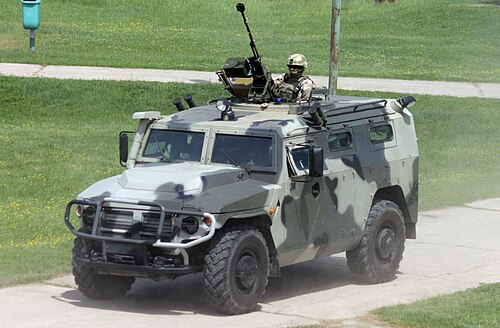
\includegraphics{../images/apc/tigr_1.jpg}
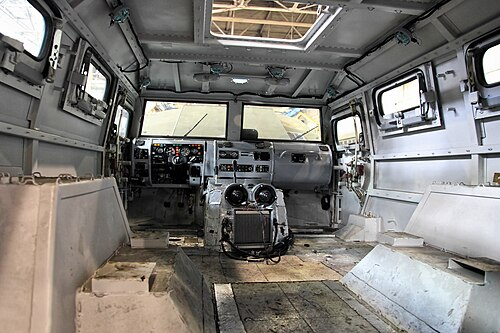
\includegraphics{../images/apc/tigr_2.jpg}

\begin{center}\rule{0.5\linewidth}{0.5pt}\end{center}

\subsection{Opis}\label{opis-17}

GAZ Tigr to rosyjski lekki pojazd wielozadaniowy produkowany przez
Gorkowską Fabrykę Samochodów (GAZ) od 2006 roku. Pełni funkcję
odpowiednika amerykańskiego Humvee, służąc jako pojazd zwiadowczy,
transportowy i patrolowy. Tigr jest powszechnie stosowany przez armię
rosyjską, jednostki Rosgwardii, Spetsnaz oraz FSB. Pojazd występuje w
wielu wariantach --- od otwartej platformy z CKM po wersję opancerzoną z
modułowym uzbrojeniem. W konfliktach w Syrii i Ukrainie Tigr stał się
jednym z najbardziej rozpoznawalnych rosyjskich pojazdów taktycznych,
choć jego opancerzenie okazało się niewystarczające wobec nowoczesnej
broni przeciwpancernej.

\subsection{Dane techniczne}\label{dane-techniczne-17}

\begin{longtable}[]{@{}
  >{\raggedright\arraybackslash}p{(\columnwidth - 2\tabcolsep) * \real{0.5263}}
  >{\raggedright\arraybackslash}p{(\columnwidth - 2\tabcolsep) * \real{0.4737}}@{}}
\toprule\noalign{}
\begin{minipage}[b]{\linewidth}\raggedright
Parametr
\end{minipage} & \begin{minipage}[b]{\linewidth}\raggedright
Wartość
\end{minipage} \\
\midrule\noalign{}
\endhead
\bottomrule\noalign{}
\endlastfoot
Typ & Lekki pojazd wielozadaniowy / MRAP \\
Kraj produkcji & Rosja \\
Rok wprowadzenia & 2006 \\
Masa bojowa & 7 200 kg \\
Długość & 5,67 m \\
Szerokość & 2,2 m \\
Wysokość & 2,0 m \\
Uzbrojenie & 7,62 mm PKP, 12,7 mm Kord lub 30 mm AGS-17 (zależnie od
wersji) \\
Silnik & YaMZ-5347-10 turbodiesel, 215 KM \\
Prędkość maks. (droga) & 140 km/h \\
Zasięg & 1 000 km \\
Załoga + pasażerowie & 2 + 9--11 osób \\
Napęd & 4×4 \\
\end{longtable}

\subsection{Charakterystyczne cechy
rozpoznawcze}\label{charakterystyczne-cechy-rozpoznawcze-17}

\begin{quote}
Jak odróżnić GAZ Tigr od innych rosyjskich pojazdów:
\end{quote}

\begin{itemize}
\tightlist
\item
  \textbf{Charakterystyczna prostokątna sylwetka z wysoką kabiną:} Tigr
  ma wyraźnie prostokątny, ``pudełkowy'' kształt nadwozia z pionowymi
  drzwiami --- odróżnia go od bardziej opływowych pojazdów NATO
\item
  \textbf{Duże okrągłe reflektory z przodu:} charakterystyczne okrągłe
  reflektory główne z przodu maski --- wyraźna cecha rozpoznawcza
  odróżniająca od pojazdów z prostokątnymi reflektorami
\item
  \textbf{Wysoki prześwit i duże terenowe opony:} znaczny prześwit
  podwozia i szerokie opony terenowe widoczne z każdej strony --- pojazd
  sprawia wrażenie ``siedzącego wysoko''
\item
  \textbf{Moduł uzbrojenia na dachu (wieżyczka lub postument):}
  większość wariantów bojowych ma wyraźny moduł z uzbrojeniem na dachu
  --- otwarta platforma lub zamknięta wieżyczka
\item
  \textbf{Brak opancerzenia bocznych drzwi (wersja podstawowa):}
  podstawowy Tigr ma cienkie drzwi bez widocznych płyt pancernych,
  dopiero wersja Tigr-M ma wzmocnione boki
\item
  \textbf{Kratka wlotu powietrza na masce:} charakterystyczna pozioma
  kratka wentylacyjna silnika z przodu maski --- wyraźna cecha górnej
  powierzchni maski
\end{itemize}

\subsection{Ciekawostka}\label{ciekawostka-17}

\begin{quote}
GAZ Tigr pierwotnie był projektowany jako pojazd cywilny do sprzedaży
eksportowej --- pierwszym zainteresowanym była armia Jordanii, która
zamówiła wersję militarną. Dopiero sukces eksportowy skłonił rosyjskie
ministerstwo obrony do zamówienia go dla własnych sił zbrojnych.
Paradoksalnie jeden z najbardziej rozpoznawalnych symboli rosyjskiego
wojska zaczynał jako projekt handlowy nastawiony na eksport, a nie na
potrzeby własnej armii.
\end{quote}

\section{2S19 Msta-S --- 152 mm armatohaubica
samobieżna}\label{s19-msta-s-152-mm-armatohaubica-samobieux17cna}

\subsubsection{2S19 Msta-S Self-Propelled Howitzer \textbar{} 2С19
«Мста-С»}\label{s19-msta-s-self-propelled-howitzer-2ux44119-ux43cux441ux442ux430-ux441}

\begin{figure}
\centering
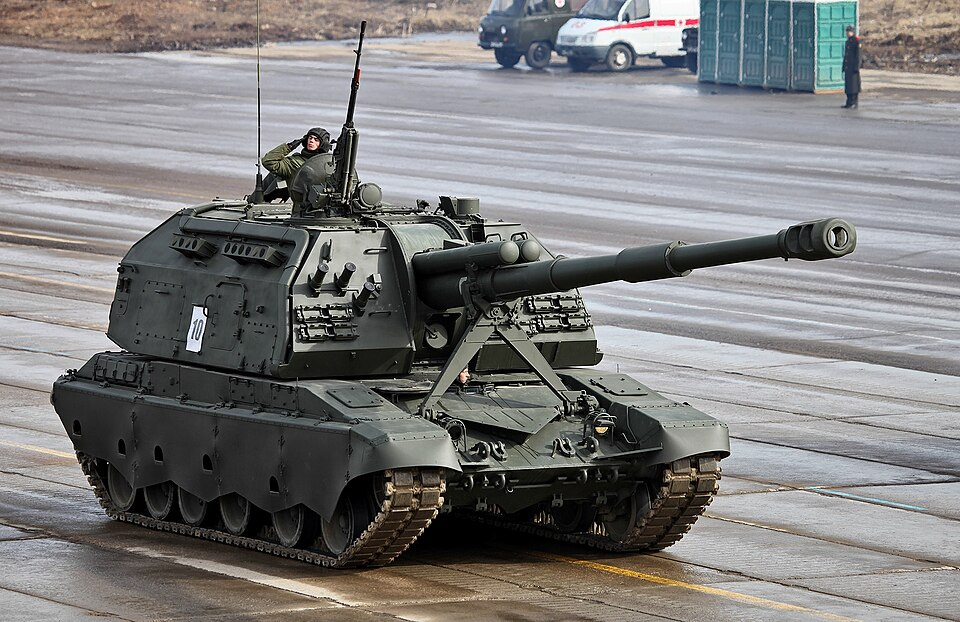
\includegraphics{../images/artyleria_samobiezna/2s19-msta-s_1.jpg}
\caption{2S19 Msta-S --- widok z boku}
\end{figure}

\begin{center}\rule{0.5\linewidth}{0.5pt}\end{center}

\subsection{Opis}\label{opis-18}

2S19 Msta-S to rosyjska 152 mm armatohaubica samobieżna, wprowadzona do
służby w 1989 roku jako następca 2S3 Akacja. Oparta na podwoziu czołgu
T-80 z silnikiem V-84A z T-72, należy do głównych systemów
artyleryjskich Sił Zbrojnych FR. Działo 2A64 osiąga donośność do 29 km
standardową amunicją (40 km z napędem rakietowym). Wyposażona w
automatyczny system ładowania (6--8 strz./min), lemiesz do okopywania
się, snorkel i generator dymu. Ponosi rekordowe straty w Ukrainie --- do
połowy 2025 roku Rosja straciła ponad 246 pojazdów tego typu.

\subsection{Dane techniczne}\label{dane-techniczne-18}

\begin{longtable}[]{@{}ll@{}}
\toprule\noalign{}
Parametr & Wartość \\
\midrule\noalign{}
\endhead
\bottomrule\noalign{}
\endlastfoot
Typ & Armatohaubica samobieżna 152 mm \\
Kraj produkcji & ZSRR / Rosja \\
Rok wprowadzenia & 1989 \\
Masa bojowa & 42 t \\
Długość kadłuba & 7,15 m \\
Szerokość & 3,38 m \\
Wysokość & 2,99 m \\
Uzbrojenie główne & Armatohaubica 152 mm 2A64 (lf. 47 kal.) \\
Donośność & 24,7 km (std.) / 29 km (base-bleed) / 36--40 km (RA) \\
Szybkostrzelność & 6--8 strz./min (2S19M2: 10 strz./min) \\
Uzbrojenie pomocnicze & WKCKM 12,7 mm NSVT (plot.) \\
Silnik & V-84A diesel, 840 KM \\
Prędkość maks. & 60 km/h \\
Zasięg & 500 km \\
Pancerz & 15 mm stal (ochrona przed odłamkami i bronią strzelecką) \\
Załoga & 5 osób \\
\end{longtable}

\subsection{Charakterystyczne cechy
rozpoznawcze}\label{charakterystyczne-cechy-rozpoznawcze-18}

\begin{quote}
Jak odróżnić 2S19 od 2S3 Akacja i innych armatohaubic:
\end{quote}

\begin{itemize}
\tightlist
\item
  \textbf{Masywna, kwadratowa wieża z charakterystycznym prostokątnym
  profilem} --- wieża 2S19 jest wyraźnie wyższa i bardziej kancista niż
  niska kopuła wieży 2S3; przypomina odwrócone pudło
\item
  \textbf{Długa lufa 152 mm z hamulcem wylotowym i osłoną termiczną} ---
  lufa ze specyficznym wielokomorowym hamulcem na końcu, wyraźnie
  dłuższa niż w 2S3
\item
  \textbf{Podwozie z 6 dużymi kołami nośnymi} --- identyczne jak
  T-72/T-80, które wyraźnie odróżnia go od 2S3 (podwozie SO-152 z 6
  kołami mniejszymi)
\item
  \textbf{WKCKM 12,7 mm na dachu wieży} --- widoczny karabin maszynowy
  na podstawie obrotowej z prawej strony włazu dowódcy
\item
  \textbf{Lemiesz spycharkowy z tyłu kadłuba} --- składana łopata
  widoczna pod tylną ścianą kadłuba
\end{itemize}

\subsection{Ciekawostka}\label{ciekawostka-18}

\begin{quote}
Na bazie podwozia 2S19 zbudowano prototyp ``1K17 Szhatie'' --- czołg
laserowy uzbrojony w baterię laserów do niszczenia optyki przeciwnika.
Rosjanie stracili w Ukrainie ponad 246 egzemplarzy Msta-S, a Ukraińcy
przerabiają uszkodzone wozy na transportery opancerzone lub montują na
nich wieże T-72 (tzw. ``FrankenMsta''). System był intensywnie używany w
bitwie o Bachmut po obu stronach.
\end{quote}

\section{Haubica samobieżna 2S1
Goździk}\label{haubica-samobieux17cna-2s1-goux17adzik}

\subsubsection{2S1 Gvozdika Self-Propelled Howitzer \textbar{} 2С1
«Гвоздика»}\label{s1-gvozdika-self-propelled-howitzer-2ux4411-ux433ux432ux43eux437ux434ux438ux43aux430}

\begin{figure}
\centering
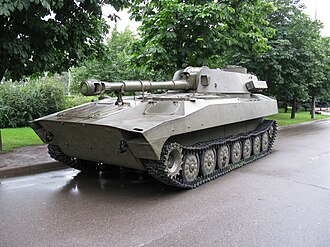
\includegraphics{../images/artyleria_samobiezna/2s1_1.jpg}
\caption{2S1 Gvozdika --- eksponat muzealny, Wzgórze Pokłonnaja Moskwa}
\end{figure}

\begin{center}\rule{0.5\linewidth}{0.5pt}\end{center}

\subsection{Opis}\label{opis-19}

2S1 Goździk (ros. «Гвоздика» --- goździk) to radziecka 122 mm haubica
samobieżna opracowana w latach 60. XX wieku i wprowadzona do służby w
1972 roku. Zbudowana na podwoziu MT-LBu, wyposażona jest w pełni
obrotową wieżę z haubicą 2A18. Posiada zdolność amfibijną --- może
przepływać rzeki bez przygotowania inżynieryjnego dzięki uszczelnieniu
kadłuba i użyciu gąsienic jako napędu wodnego. Goździk jest jednym z
najszerzej eksportowanych radzieckich dział samobieżnych --- służy w
ponad 30 armiach świata i był intensywnie stosowany w wojnie w Ukrainie
po obu stronach konfliktu.

\subsection{Dane techniczne}\label{dane-techniczne-19}

\begin{longtable}[]{@{}ll@{}}
\toprule\noalign{}
Parametr & Wartość \\
\midrule\noalign{}
\endhead
\bottomrule\noalign{}
\endlastfoot
Typ & Samobieżna haubica gąsienicowa \\
Kraj produkcji & ZSRR / Rosja \\
Rok wprowadzenia & 1972 \\
Masa bojowa & 16 t \\
Długość (z lufą) & 7,26 m \\
Szerokość & 2,85 m \\
Wysokość & 2,73 m \\
Uzbrojenie główne & Haubica 122 mm 2A18 \\
Zasięg strzału & do 15,3 km (standardowy), do 21,9 km (RAP) \\
Szybkostrzelność & 4--5 strz./min \\
Silnik & YaMZ-238N diesel, 300 KM \\
Prędkość maks. & 60 km/h \\
Zasięg & 500 km \\
Załoga & 4 osoby \\
\end{longtable}

\subsection{Charakterystyczne cechy
rozpoznawcze}\label{charakterystyczne-cechy-rozpoznawcze-19}

\begin{quote}
Jak odróżnić 2S1 od innych dział samobieżnych:
\end{quote}

\begin{itemize}
\tightlist
\item
  \textbf{Niska, zaokrąglona wieża na szerokim kadłubie:} wieża 2S1 jest
  stosunkowo niska i okrągła w planie, osadzona na charakterystycznym
  szerokim, płaskim kadłubie MT-LBu
\item
  \textbf{Krótka, gruba lufa 122 mm z hamulcem wylotowym:} lufa jest
  wyraźnie krótsza i grubsza niż w 2S3 (152 mm) --- z charakterystycznym
  dwukomorowym hamulcem wylotowym
\item
  \textbf{Szerokie gąsienice i niski profil:} podwozie MT-LBu ma
  wyjątkowo szerokie gąsienice (szersze niż podwozia czołgów) i bardzo
  niski profil całego pojazdu
\item
  \textbf{Brak osłony przeciwodłamkowej lufy (typowo):} standardowa
  wersja 2S1 nie ma termicznej osłony lufy, co odróżnia ją od nowszych
  systemów
\item
  \textbf{Okrągły komin/wentylator na lewej stronie wieży:}
  charakterystyczny okrągły otwór wentylacyjny po lewej stronie wieży to
  stały element 2S1
\item
  \textbf{Małe koła jezdne (7 kół po każdej stronie):} podwozie MT-LBu
  ma 7 małych kółek jezdnych --- wyraźnie więcej niż typowe podwozia
  czołgów z 6 kołami
\end{itemize}

\subsection{Ciekawostka}\label{ciekawostka-19}

\begin{quote}
Goździk jest jednym z niewielu dział samobieżnych zdolnych do pływania
bez żadnego przygotowania --- szczelność kadłuba jest tak dobra, że
pojazd może wjechać bezpośrednio do rzeki i przepłynąć na drugi brzeg
używając gąsienic jako wioseł. Prędkość pływania wynosi około 4,5 km/h.
Ta cecha okazała się nieoceniona podczas przekraczania licznych rzek w
Ukrainie i Syrii.
\end{quote}

\section{Haubica samobieżna 2S3
Akacja}\label{haubica-samobieux17cna-2s3-akacja}

\subsubsection{2S3 Akatsiya Self-Propelled Howitzer \textbar{} 2С3
«Акация»}\label{s3-akatsiya-self-propelled-howitzer-2ux4413-ux430ux43aux430ux446ux438ux44f}

\begin{figure}
\centering
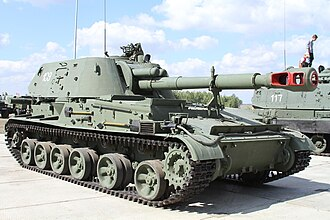
\includegraphics{../images/artyleria_samobiezna/2s3_1.jpg}
\caption{2S3 Akatsiya --- eksponat muzealny}
\end{figure}

\begin{center}\rule{0.5\linewidth}{0.5pt}\end{center}

\subsection{Opis}\label{opis-20}

2S3 Akacja (ros. «Акация» --- akacja) to radziecka 152 mm haubica
samobieżna opracowana w 1968 roku i wprowadzona do służby w 1971 roku.
Stanowi odpowiedź na zachodnie systemy artylerii samobieżnej i przez
dekady była podstawową haubicą samobieżną Wojsk Lądowych ZSRR i Rosji.
Zbudowana na specjalnym podwoziu gąsienicowym z w pełni zamkniętą,
obrotową wieżą. Pojazd może strzelać pociskami standardowymi,
rakietowymi wspomaganymi (RAP), a także nuklearnymi pociskami
taktycznymi. Akacja jest wciąż szeroko stosowana w armii rosyjskiej i
była intensywnie używana w Syrii i Ukrainie.

\subsection{Dane techniczne}\label{dane-techniczne-20}

\begin{longtable}[]{@{}ll@{}}
\toprule\noalign{}
Parametr & Wartość \\
\midrule\noalign{}
\endhead
\bottomrule\noalign{}
\endlastfoot
Typ & Samobieżna haubica gąsienicowa \\
Kraj produkcji & ZSRR / Rosja \\
Rok wprowadzenia & 1971 \\
Masa bojowa & 27,5 t \\
Długość (z lufą) & 8,4 m \\
Szerokość & 3,25 m \\
Wysokość & 3,05 m \\
Uzbrojenie główne & Haubica 152,4 mm D-22 \\
Zasięg strzału & do 24 km (standardowy), do 30 km (RAP) \\
Szybkostrzelność & 3--4 strz./min \\
Silnik & W-59 diesel, 520 KM \\
Prędkość maks. & 63 km/h \\
Zasięg & 500 km \\
Załoga & 4--6 osób \\
\end{longtable}

\subsection{Charakterystyczne cechy
rozpoznawcze}\label{charakterystyczne-cechy-rozpoznawcze-20}

\begin{quote}
Jak odróżnić 2S3 od 2S1 i innych haubic samobieżnych:
\end{quote}

\begin{itemize}
\tightlist
\item
  \textbf{Duża, walcowata wieża z długą lufą 152 mm:} wieża 2S3 jest
  wyraźnie większa i wyższa niż 2S1 --- długa lufa 152 mm z typowym
  cylindrycznym hamulcem wylotowym jednoznacznie identyfikuje ten system
\item
  \textbf{Wysoka sylwetka pojazdu (3,05 m):} 2S3 jest wyraźnie wyższy od
  2S1 --- sylwetka bardziej przypomina czołg niż niski transporter
\item
  \textbf{Prostokątna tylna część kadłuba z drzwiami:} z tyłu kadłuba
  widoczne są duże drzwi ładunkowe --- przez które uzupełnia się
  amunicję --- typowy element 2S3
\item
  \textbf{Charakterystyczny kształt wieży --- cylindryczna z płaskim
  dachem:} wieża ma kształt niemal idealnego walca z płaskim dachem i
  licznymi włazami
\item
  \textbf{6 kół jezdnych na gąsienicach z dużymi lukami:} podwozie ma 6
  kół jezdnych na każdej stronie z wyraźnymi przestrzeniami między nimi
\item
  \textbf{Antena radiowa na prawej stronie wieży:} długa pałąkowa lub
  sztyftowa antena radiostacji stoi typowo po prawej tylnej stronie
  wieży
\end{itemize}

\subsection{Ciekawostka}\label{ciekawostka-20}

\begin{quote}
2S3 jest jednym z niewielu systemów artylerii samobieżnej
zaprojektowanych do strzelania taktyczną bronią nuklearną --- specjalny
pocisk jądrowy 3BV2 (kaliber 152 mm) mógł być odpalany ze standardowej
lufy systemu. Procedura strzelania jądrowego wymagała jednak ewakuacji
obszaru w promieniu kilkuset metrów od pojazdu przed strzałem ze względu
na promieniowanie własnego ładunku.
\end{quote}

\section{Armata samobieżna 2S5
Hiacynt-S}\label{armata-samobieux17cna-2s5-hiacynt-s}

\subsubsection{2S5 Giatsint-S Self-Propelled Gun \textbar{} 2С5
«Гиацинт-С»}\label{s5-giatsint-s-self-propelled-gun-2ux4415-ux433ux438ux430ux446ux438ux43dux442-ux441}

\begin{figure}
\centering
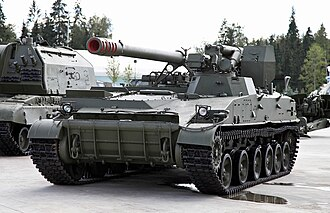
\includegraphics{../images/artyleria_samobiezna/2s5_1.jpg}
\caption{2S5 Giatsint-S --- ekspozycja w Parku Patriot}
\end{figure}

\begin{center}\rule{0.5\linewidth}{0.5pt}\end{center}

\subsection{Opis}\label{opis-21}

2S5 Hiacynt-S (ros. «Гиацинт-С» --- hiacynt samobieżny) to radziecka 152
mm armata samobieżna o wyjątkowo dużym zasięgu, wprowadzona do służby w
1978 roku. W odróżnieniu od haubic 2S1 i 2S3 jest to armata (działo o
długiej lufie i wysokiej prędkości początkowej pocisku), co daje jej
zasięg do 28 km pociskami standardowymi i aż 40 km pociskami rakietowo
wspomaganymi. System jest przeznaczony do zwalczania głęboko
rozmieszczonych celów w tylach wroga --- stanowisk dowodzenia, składów
amunicji i węzłów komunikacyjnych. Lufa i mechanizm ładowania są
umieszczone na otwartym tylnym stanowisku (bez wieży), co odróżnia
Hiacynt-S od większości innych dział samobieżnych.

\subsection{Dane techniczne}\label{dane-techniczne-21}

\begin{longtable}[]{@{}ll@{}}
\toprule\noalign{}
Parametr & Wartość \\
\midrule\noalign{}
\endhead
\bottomrule\noalign{}
\endlastfoot
Typ & Samobieżna armata gąsienicowa \\
Kraj produkcji & ZSRR / Rosja \\
Rok wprowadzenia & 1978 \\
Masa bojowa & 28,2 t \\
Długość & 8,33 m \\
Uzbrojenie główne & Armata 152 mm 2A37 (lufa L/54) \\
Zasięg strzału & do 28 km (standardowy), do 40 km (RAP) \\
Szybkostrzelność & 5--6 strz./min \\
Amunicja & 30 nabojów w pojeździe \\
Silnik & diesel, 520 KM \\
Prędkość maks. & 62 km/h \\
Zasięg & 500 km \\
Załoga & 5 osób \\
\end{longtable}

\subsection{Charakterystyczne cechy
rozpoznawcze}\label{charakterystyczne-cechy-rozpoznawcze-21}

\begin{quote}
Jak odróżnić 2S5 od 2S3 i innych dział samobieżnych:
\end{quote}

\begin{itemize}
\tightlist
\item
  \textbf{Brak zamkniętej wieży --- otwarte stanowisko ogniowe z tyłu:}
  2S5 nie ma wieży! Działo i obsługa są całkowicie odkryte z tyłu
  pojazdu --- to natychmiastowy odróżnik od 2S3 (pełna wieża) i 2S1
\item
  \textbf{Wyjątkowo długa lufa (L/54):} lufa 2S5 jest wyraźnie dłuższa
  proporcjonalnie do pojazdu niż w 2S3 --- sięga daleko przed przód
  kadłuba i jest cienka (armata, nie haubica)
\item
  \textbf{Duża tarcza ochronna przy lufie:} przed stanowiskiem obsługi
  stoi charakterystyczna prostokątna tarcza stalowa chroniąca załogę
  przed odłamkami z przodu
\item
  \textbf{Kadłub podobny do 2S3 ale bez wieży:} podwozie i kadłub 2S5 są
  podobne do 2S3, ale górna część pojazdu jest płaska z otwartą
  platformą z tyłu
\item
  \textbf{Dwa ramiona hydrauliczne do stabilizacji:} z tyłu kadłuba
  opuszczane są dwa duże lemiesze/ramiona hydrauliczne wbijające się w
  ziemię dla stabilizacji podczas strzelania
\item
  \textbf{Długi wysięgnik ładowania amunicji:} automatyczny podajnik
  amunicji z tyłu pojazdu to charakterystyczny element --- duże ramię
  mechaniczne ładujące naboje kaliber 152 mm
\end{itemize}

\subsection{Ciekawostka}\label{ciekawostka-21}

\begin{quote}
2S5 był jednym z pierwszych radzieckich systemów artylerii zdolnych do
strzelania pociskami z samonaprowadzaniem laserowym Krasnopol ---
specjalnym pociskiem 152 mm, który po wystrzale sam naprowadza się na
cel podświetlony laserem przez obserwatora naziemnego lub drona. Jeden
pocisk Krasnopol kosztuje wielokrotnie więcej niż standardowy, ale
gwarantuje trafienie w pojazd lub bunkier z pierwszego strzału.
\end{quote}

\section{Moździerz samobieżny 2S9
Nona-S}\label{moux17adzierz-samobieux17cny-2s9-nona-s}

\subsubsection{2S9 Nona-S Self-Propelled Mortar \textbar{} 2С9
«Нона-С»}\label{s9-nona-s-self-propelled-mortar-2ux4419-ux43dux43eux43dux430-ux441}

\begin{figure}
\centering
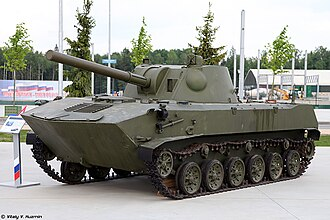
\includegraphics{../images/artyleria_samobiezna/2s9_1.jpg}
\caption{2S9 Nona-S --- ekspozycja w Parku Patriot}
\end{figure}

\begin{center}\rule{0.5\linewidth}{0.5pt}\end{center}

\subsection{Opis}\label{opis-22}

2S9 Nona-S (ros. «Нона» --- skrót od „Nowoje Orużije Naziemnoj
Artillerii'') to radziecka 120 mm samobieżna haubico-moździerzo-armata,
wprowadzona do służby w 1981 roku. Zbudowana na podwoziu BTR-D (lotnicza
wersja BMD), jest jednym z nielicznych systemów artylerii zdolnych do
desantowania ze śmigłowca lub samolotu transportowego. System łączy
cechy moździerza, haubicy i armaty --- może prowadzić ogień pośredni jak
moździerz, bezpośredni jak armata przeciwpancerna oraz strzelać
pociskami kierowanymi. Jest powszechnie stosowana przez rosyjskie wojska
powietrznodesantowe (VDV).

\subsection{Dane techniczne}\label{dane-techniczne-22}

\begin{longtable}[]{@{}ll@{}}
\toprule\noalign{}
Parametr & Wartość \\
\midrule\noalign{}
\endhead
\bottomrule\noalign{}
\endlastfoot
Typ & Samobieżna haubico-moździerzo-armata 120 mm \\
Kraj produkcji & ZSRR / Rosja \\
Rok wprowadzenia & 1981 \\
Masa bojowa & 8,7 t \\
Uzbrojenie główne & 120 mm 2A60 (haubico-moździerz) \\
Zasięg strzału & do 8,8 km (standardowy), do 12,8 km (RAP) \\
Szybkostrzelność & 8--10 strz./min \\
Silnik & 5D20 diesel, 240 KM \\
Prędkość maks. & 60 km/h (ląd), 9 km/h (woda) \\
Zasięg & 500 km \\
Załoga & 4 osoby \\
Desant lotniczy & Tak (Il-76, An-12) \\
\end{longtable}

\subsection{Charakterystyczne cechy
rozpoznawcze}\label{charakterystyczne-cechy-rozpoznawcze-22}

\begin{quote}
Jak odróżnić 2S9 od 2S1 i innych systemów:
\end{quote}

\begin{itemize}
\tightlist
\item
  \textbf{Wyjątkowo niska, kompaktowa sylwetka:} 2S9 jest wyraźnie
  mniejsza i niższa od 2S1 --- widać to szczególnie porównując wysokość
  wieży; to bardzo ``płaski'' pojazd
\item
  \textbf{Podwozie gąsienicowe bez kół bocznych (płazy):} podwozie BTR-D
  ma charakterystyczne małe koła jezdne bez górnego podparcia gąsienicy
  --- gąsienica ``wisi'' bez rolek nośnych
\item
  \textbf{Mała okrągła wieża z krótką lufą 120 mm:} wieża jest bardzo
  mała i okrągła z krótką grubą lufą o kalibrze 120 mm --- bez hamulca
  wylotowego (moździerz gładkolufowy)
\item
  \textbf{Tylna klapa desantowa:} z tyłu kadłuba widoczna duża klapa z
  kratownicą wzmacniającą --- identyczna jak w BTR-D/BMD, bo 2S9 jest na
  tym samym podwoziu
\item
  \textbf{Brak hamulca wylotowego na lufie:} lufa 2S9 kończy się gładko
  bez żadnego urządzenia wylotowego --- charakterystyczne dla moździerzy
  gładkolufowych
\item
  \textbf{Bardzo małe wymiary pojazdu:} 2S9 jest znacznie mniejsza niż
  2S1 --- widać to od razu; jest jednym z najmniejszych samobieżnych
  systemów artylerii na świecie
\end{itemize}

\subsection{Ciekawostka}\label{ciekawostka-22}

\begin{quote}
2S9 jest jedyną armatą samobieżną na świecie seryjnie desantowaną na
spadochronie razem z załogą w środku. Procedura PDSS (Para-Desant ze
Składu Środka) polega na tym, że załoga siedzi w pojeździe, który jest
wyrzucany z samolotu na wysokości kilkuset metrów i ląduje na
wielostopniowym systemie rakietowo-spadochronowym. System ten działa od
ponad 30 lat, choć rosyjscy spadochroniarze żartują, że zawsze wolą
desantować się osobno.
\end{quote}

\section{Moździerz samobieżny 2S23
Nona-SVK}\label{moux17adzierz-samobieux17cny-2s23-nona-svk}

\subsubsection{2S23 Nona-SVK Self-Propelled Mortar \textbar{} 2С23
«Нона-СВК»}\label{s23-nona-svk-self-propelled-mortar-2ux44123-ux43dux43eux43dux430-ux441ux432ux43a}

\begin{figure}
\centering
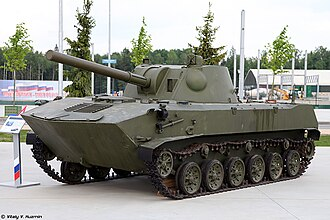
\includegraphics{../images/artyleria_samobiezna/2s23_1.jpg}
\caption{2S23 Nona-SVK --- ekspozycja w Parku Patriot}
\end{figure}

\begin{center}\rule{0.5\linewidth}{0.5pt}\end{center}

\subsection{Opis}\label{opis-23}

2S23 Nona-SVK (ros. «Нона-СВК» --- Nowoje Orużije Naziemnoj Artillerii,
Samochódnaja Wintowaja Kołiesnaja) to rosyjski 120 mm samobieżny
moździerz-armata na podwoziu kołowym BTR-80, wprowadzony do służby w
1990 roku. Jest kołową wersją gąsienicowej 2S9 Nona-S i przeznaczony dla
jednostek zmotoryzowanych (nie powietrznodesantowych). Zastosowanie
podwozia BTR-80 (8×8) daje większą mobilność drogową i prostszą
logistykę niż wersja gąsienicowa. System może prowadzić ogień na
wszystkie strony bez zawracania pojazdu, z zasięgiem do 12,8 km.
Stosowany przez armię rosyjską i jednostki zmotoryzowane.

\subsection{Dane techniczne}\label{dane-techniczne-23}

\begin{longtable}[]{@{}ll@{}}
\toprule\noalign{}
Parametr & Wartość \\
\midrule\noalign{}
\endhead
\bottomrule\noalign{}
\endlastfoot
Typ & Samobieżny moździerz-armata kołowy 120 mm \\
Kraj produkcji & Rosja \\
Rok wprowadzenia & 1990 \\
Masa bojowa & 14,5 t \\
Uzbrojenie główne & 120 mm 2A60 (haubico-moździerz) \\
Zasięg strzału & do 8,8 km (standardowy), do 12,8 km (RAP) \\
Szybkostrzelność & 8--10 strz./min \\
Pojazd bazowy & BTR-80 (kołowy 8×8) \\
Prędkość maks. & 80 km/h \\
Zasięg & 600 km \\
Załoga & 4 osoby \\
\end{longtable}

\subsection{Charakterystyczne cechy
rozpoznawcze}\label{charakterystyczne-cechy-rozpoznawcze-23}

\begin{quote}
Jak odróżnić 2S23 od 2S9 i BTR-80:
\end{quote}

\begin{itemize}
\tightlist
\item
  \textbf{Kołowe podwozie BTR-80 z wieżą zamiast standardowej
  wieżyczki:} od razu widać, że to pojazd kołowy (8 kół) z
  charakterystyczną wieżą moździerza zamiast typowej wieżyczki CKM
  BTR-80
\item
  \textbf{Krótka, gruba lufa 120 mm z wieży na środku pojazdu:} z górnej
  części kadłuba wyrasta wieża z krótką grubą lufą skierowaną ku górze
  lub lekko do przodu --- inna proporcja niż długa lufa armat
\item
  \textbf{Sylwetka BTR-80 z ``naroślem'' wieżowym:} kadłub jest
  identyczny z BTR-80 --- ``pochylony nos'', 8 kół, boczne drzwi
  desantowe --- tylko wieżyczka jest inna
\item
  \textbf{Brak hamulca wylotowego na lufie:} lufa jest gładka na końcu
  (moździerz gładkolufowy) --- w odróżnieniu od haubic i armat z
  hamulcami wylotowymi
\item
  \textbf{Obrót wieży o 360°:} wieża może się obracać dookoła --- widać
  to jako oddzielna, duża konstrukcja na kadłubie BTR
\item
  \textbf{Antena radiostacji na tyłach wieży:} charakterystyczna długa
  antena z tyłu lub boku wieży --- taka sama jak w wersji bojowej BTR-80
\end{itemize}

\subsection{Ciekawostka}\label{ciekawostka-23}

\begin{quote}
2S23 jest jedynym rosyjskim systemem artyleryjskim kołowym zdolnym do
pływania --- podwozie BTR-80 zachowuje swoje zdolności amfibijne nawet z
wieżą moździerza. Oznacza to, że cała bateria 2S23 może przepłynąć rzekę
bez pontonu i zaraz po wyjściu z wody prowadzić ogień. Ta cecha bywa
niedoceniana, ale okazała się cenna przy forsowaniu rzek w wielu
konfliktach zbrojnych.
\end{quote}

\section{Moździerz samobieżny 2S4
Tulipan}\label{moux17adzierz-samobieux17cny-2s4-tulipan}

\subsubsection{2S4 Tyulpan Self-Propelled Mortar \textbar{} 2С4
«Тюльпан»}\label{s4-tyulpan-self-propelled-mortar-2ux4414-ux442ux44eux43bux44cux43fux430ux43d}

\begin{figure}
\centering
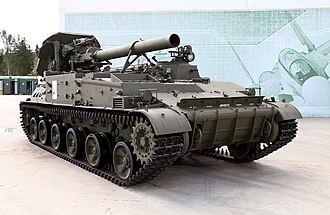
\includegraphics{../images/artyleria_samobiezna/2s4_1.jpg}
\caption{2S4 Tyulpan --- ekspozycja w Parku Patriot}
\end{figure}

\begin{center}\rule{0.5\linewidth}{0.5pt}\end{center}

\subsection{Opis}\label{opis-24}

2S4 Tulipan (ros. «Тюльпан» --- tulipan) to radziecki 240 mm moździerz
samobieżny --- największy system moździerzowy będący w służbie wojskowej
na świecie. Wprowadzony do służby w 1975 roku, przeznaczony jest do
niszczenia silnie ufortyfikowanych pozycji obronnych, bunkrów
żelbetowych i skupisk wojsk. Pocisk 240 mm waży do 130 kg i może
przenosić głowicę nuklearną, chemiczną lub termobaryczną. Tulipan był
używany w Afganistanie do niszczenia jaskiń i fortec mudżahedinów, w
Czeczenii do burzenia bloków mieszkalnych oraz w Ukrainie do atakowania
miast. Ze względu na niszczycielską siłę rażenia jest nazywany przez
żołnierzy ``pociągiem śmierci''.

\subsection{Dane techniczne}\label{dane-techniczne-24}

\begin{longtable}[]{@{}ll@{}}
\toprule\noalign{}
Parametr & Wartość \\
\midrule\noalign{}
\endhead
\bottomrule\noalign{}
\endlastfoot
Typ & Samobieżny moździerz 240 mm \\
Kraj produkcji & ZSRR / Rosja \\
Rok wprowadzenia & 1975 \\
Masa bojowa & 27,5 t \\
Uzbrojenie główne & 240 mm moździerz gładkolufowy 2B8 \\
Zasięg strzału & 800 m -- 18 000 m \\
Masa pocisku & do 130 kg \\
Szybkostrzelność & 1 strz./min \\
Amunicja & 40 pocisków standardowych / 20 RAP \\
Prędkość maks. & 60 km/h \\
Załoga & 4 (w pojeździe) + 5 (w pojeździe wsparcia) \\
\end{longtable}

\subsection{Charakterystyczne cechy
rozpoznawcze}\label{charakterystyczne-cechy-rozpoznawcze-24}

\begin{quote}
Jak odróżnić 2S4 od innych dział samobieżnych:
\end{quote}

\begin{itemize}
\tightlist
\item
  \textbf{Ogromna lufa 240 mm z tyłu pojazdu --- wycelowana ku górze:} w
  pozycji marszowej gigantyczna lufa jest złożona wzdłuż kadłuba; w
  pozycji bojowej jest pionowo uniesiona ku górze --- wygląda jak wielki
  komin
\item
  \textbf{Ładowanie pocisku z tyłu na ziemi:} w odróżnieniu od innych
  dział, Tulipan ładuje się podając pocisk od tyłu kadłuba na specjalny
  tacę --- widać to wyraźnie na zdjęciach z ćwiczeń
\item
  \textbf{Masywne lemiesze stabilizujące z tyłu:} w pozycji bojowej z
  tyłu pojazdu opuszczane są dwa ogromne lemiesze wbijające się głęboko
  w ziemię --- niezbędne przy odrzucie strzału 240 mm
\item
  \textbf{Brak wieży --- otwarta platforma z tyłu:} górna tylna część
  2S4 jest całkowicie otwarta --- moździerz stoi na odkrytej platformie,
  obsługa pracuje na zewnątrz przy każdym strzale
\item
  \textbf{Krótki, masywny kadłub bez wystającej lufy z przodu:} w
  pozycji marszowej lufa leży wzdłuż kadłuba, więc pojazd wygląda jak
  ``pudełko z tyłu'' --- inaczej niż 2S3 czy 2S5 z wystającą do przodu
  lufą
\item
  \textbf{Podwozie podobne do 2S3 ale wyraźnie cięższe:} 2S4 jest o
  podobnej długości co 2S3, ale masywniejszy, z głębiej osadonymi
  gąsienicami i większym prześwitem
\end{itemize}

\subsection{Ciekawostka}\label{ciekawostka-24}

\begin{quote}
W Afganistanie jeden Tulipan zużył tyle amunicji do niszczenia jednej
jaskini, ile normalnie wystarczyłoby na tygodniową bitwę. Lokalni
mieszkańcy nazywali go ``bogiem wojny'' --- nie z podziwu, ale ze
strachu. Jeden pocisk 3F2 (termobaryczny) wypełnia sferyczną falą
uderzeniową przestrzeń o objętości budynku mieszkalnego, zabijając
wszystkich wewnątrz przez nadciśnienie --- bez konieczności
bezpośredniego trafienia.
\end{quote}

\section{Moździerz samobieżny 2S40
Floks}\label{moux17adzierz-samobieux17cny-2s40-floks}

\subsubsection{2S40 Floks Self-Propelled Mortar \textbar{} 2С40
«Флокс»}\label{s40-floks-self-propelled-mortar-2ux44140-ux444ux43bux43eux43aux441}

\begin{center}\rule{0.5\linewidth}{0.5pt}\end{center}

\subsection{Opis}\label{opis-25}

2S40 Floks (ros. «Флокс» --- floks) to rosyjski 120 mm moździerz
samobieżny na podwoziu ciężarówki Ural-4320 (6×6), oddany do służby w
2023 roku. Jest jednym z najnowszych rosyjskich systemów artylerii i
powstał jako odpowiedź na zapotrzebowanie na mobilny, tani i łatwy w
obsłudze system wsparcia ogniowego dla jednostek szczebla batalion.
Zabudowa na ciężarówce Ural zamiast specjalistycznego podwozia bojowego
radykalnie obniża koszty produkcji i upraszcza logistykę. System wziął
udział w walkach w Ukrainie już w roku jego wprowadzenia do służby.

\subsection{Dane techniczne}\label{dane-techniczne-25}

\begin{longtable}[]{@{}ll@{}}
\toprule\noalign{}
Parametr & Wartość \\
\midrule\noalign{}
\endhead
\bottomrule\noalign{}
\endlastfoot
Typ & Samobieżny moździerz kołowy 120 mm \\
Kraj produkcji & Rosja \\
Rok wprowadzenia & 2023 \\
Masa bojowa & 20 t \\
Uzbrojenie główne & 120 mm półautomatyczny gwintowany moździerz \\
Zasięg strzału & do 8,5 km (HE), do 10 km (pociski kierowane) \\
Pojazd bazowy & Ural-4320 6×6 \\
Załoga & 4 osoby \\
\end{longtable}

\subsection{Charakterystyczne cechy
rozpoznawcze}\label{charakterystyczne-cechy-rozpoznawcze-25}

\begin{quote}
Jak rozpoznać 2S40 Floks:
\end{quote}

\begin{itemize}
\tightlist
\item
  \textbf{Ciężarówka Ural z opancerzoną kabiną i modułem ogniowym z
  tyłu:} sylwetka to niezbicie ciężarówka wojskowa --- kabina Urala z
  charakterystycznym prostokątnym przodem --- z tyłu platforma z
  moździerzem
\item
  \textbf{Lufa moździerza skierowana ku górze lub złożona wzdłuż
  pojazdu:} lufa 120 mm jest widoczna z tyłu ciężarówki --- w pozycji
  marszowej złożona, w bojowej --- skierowana ku górze
\item
  \textbf{Opancerzona kabina z charakterystycznymi klinowatymi
  osłonami:} kabina Urala ma dodane prostokątne płyty pancerne po bokach
  i z przodu --- wyraźnie różni się od cywilnego Urala
\item
  \textbf{Brak gąsienic --- 6 kół terenowych Urala:} koła ciężarówki
  wojskowej Ural są natychmiastowym rozpoznaniem --- żaden inny rosyjski
  system artyleryjski nie jest na standardowej ciężarówce
\item
  \textbf{Modułowy kontener ogniowy z tyłu skrzyni:} za kabiną widoczny
  jest duży kontener/moduł z mechaniką moździerza --- inaczej niż w 2S23
  (wieża na BWP) czy 2S9 (wieża na gąsienicach)
\item
  \textbf{Anteny i skrzynki elektroniczne na dachu kabiny:} nowoczesne
  systemy nawigacji i łączności na dachu kabiny --- element
  charakterystyczny dla systemów produkowanych po 2020 roku
\end{itemize}

\subsection{Ciekawostka}\label{ciekawostka-25}

\begin{quote}
Floks był jednym z pierwszych rosyjskich systemów uzbrojenia
zaprojektowanych z myślą o wnioskami z walk w Ukrainie --- szybka budowa
na podwoziu cywilnym (Ural) zamiast wieloletniego procesu zamówień na
specjalistyczne podwozie bojowe. Od pomysłu do dostawy pierwszych
egzemplarzy minęły zaledwie 2 lata, co w rosyjskim przemyśle
zbrojeniowym jest rekordem. Analitycy NATO zwracają uwagę, że to nowy
trend: Rosja zaczyna coraz częściej stosować ``szybką produkcję'' na
bazie pojazdów cywilnych zamiast kosztownych platform bojowych.
\end{quote}

\section{Haubica holowana D-30 (2A18)}\label{haubica-holowana-d-30-2a18}

\subsubsection{D-30 122mm Towed Howitzer \textbar{} Д-30
(2А18)}\label{d-30-122mm-towed-howitzer-ux434-30-2ux43018}

\begin{figure}
\centering
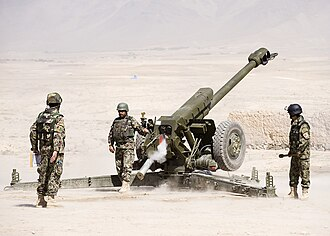
\includegraphics{../images/artyleria_holowana/d-30_1.jpg}
\caption{D-30 --- haubica podczas ćwiczeń}
\end{figure}

\begin{center}\rule{0.5\linewidth}{0.5pt}\end{center}

\subsection{Opis}\label{opis-26}

D-30 (indeks GRAU: 2A18) to radziecka 122 mm haubica holowana
zaprojektowana jako następca M-30 i wprowadzona do służby w 1960 roku.
Charakteryzuje się unikalnym trójosiowym łożem rozkładanym w kształt
trójnoga --- po rozłożeniu trzech nóg możliwe jest prowadzenie ognia
okrężnego w pełnym zakresie 360°, bez potrzeby przekładania działa. D-30
jest jedną z najbardziej udanych i wszechstronnych haubic w historii ---
produkowana w kilkudziesięciu krajach, służy w ponad 60 armiach i była
używana w niemal każdym większym konflikcie zbrojnym od lat 60. po dziś
dzień. Doskonale sprawdza się zarówno jako haubica polowa, jak i jako
broń przeciwpancerna (strzelając pociskami HEAT, przebija do 460 mm
pancerza).

\subsection{Dane techniczne}\label{dane-techniczne-26}

\begin{longtable}[]{@{}ll@{}}
\toprule\noalign{}
Parametr & Wartość \\
\midrule\noalign{}
\endhead
\bottomrule\noalign{}
\endlastfoot
Typ & Haubica holowana 122 mm \\
Kraj produkcji & ZSRR \\
Rok wprowadzenia & 1960 \\
Kaliber & 122 mm \\
Masa bojowa & 3 210 kg \\
Długość lufy & L/38 \\
Zasięg strzału & do 15,4 km (standardowy), do 21,9 km (RAP) \\
Szybkostrzelność & 5--6 strz./min (maks. 10--12) \\
Kąt ostrzału (poziomy) & 360° (po rozłożeniu łoża) \\
Obsługa & 8 osób \\
\end{longtable}

\subsection{Charakterystyczne cechy
rozpoznawcze}\label{charakterystyczne-cechy-rozpoznawcze-26}

\begin{quote}
Jak odróżnić D-30 od innych haubic holowanych:
\end{quote}

\begin{itemize}
\tightlist
\item
  \textbf{Trójnożne łoże rozłożone jak ``pająk'':} gdy D-30 jest w
  pozycji bojowej, trzy nogi łoża są rozłożone pod kątem 120° do siebie,
  tworząc charakterystyczny kształt trzech ramion --- żadna inna haubica
  nie ma identycznego układu
\item
  \textbf{Obrót o 360° bez przestawiania całego działa:} w pozycji
  bojowej D-30 można skierować w dowolną stronę bez podnoszenia nóg ---
  ta cecha jest unikalna i widoczna podczas obserwacji stanowiska
  ogniowego
\item
  \textbf{Dwa koła jezdne z przodu po złożeniu do transportu:} w pozycji
  marszowej D-30 jedzie ``nosem'' z lufą z przodu --- dwa duże koła z
  przodu, łoże złożone z tyłu za lufą
\item
  \textbf{Charakterystyczna długa osłona lufy (termiczna) --- brak lub
  obecność:} starsze D-30 nie mają osłony termicznej lufy, nowsze wersje
  i modernizacje mogą ją mieć; w obu przypadkach proporcje są
  charakterystyczne
\item
  \textbf{Niski profil działa na stanowisku ogniowym:} d-30 jest bardzo
  niska --- obsługa pracuje przy niej w pozycji półprzysiadowej; to
  wyróżnia ją od wyższych haubic zachodnich
\item
  \textbf{Dwa duże koła z grubymi oponami terenowymi:} koła transportowe
  D-30 są duże, z wyraźnym bieżnikiem terenowym --- umieszczone po
  bokach łoża głównego
\end{itemize}

\subsection{Ciekawostka}\label{ciekawostka-26}

\begin{quote}
D-30 to broń tak wszechstronna, że stała się ``jeepem artylerii'' ---
używana jest przez regularnie armie, siły nieregularne, terrorystów i
obrońców miast na całym świecie. W Syrii nagrano, jak ISIS montuje D-30
na platformie pickupa tworząc mobilne działo. W Ukrainie Obrona
Terytorialna użyła D-30 zdobytych na Rosjanach natychmiast po
przeszkoleniu w ciągu kilku godzin --- tak prosta jest w obsłudze.
Szacuje się, że na świecie istnieje ponad 12 000 sprawnych egzemplarzy
D-30.
\end{quote}

\section{Haubica polowa M-30}\label{haubica-polowa-m-30}

\subsubsection{M-30 Field Howitzer \textbar{} М-30 (122-мм гаубица обр.
1938
г.)}\label{m-30-field-howitzer-ux43c-30-122-ux43cux43c-ux433ux430ux443ux431ux438ux446ux430-ux43eux431ux440.-1938-ux433.}

\begin{center}\rule{0.5\linewidth}{0.5pt}\end{center}

\begin{figure}
\centering
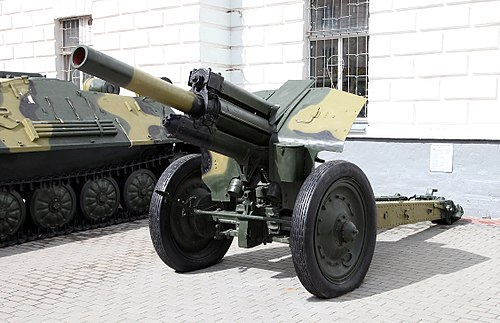
\includegraphics{../images/artyleria_holowana/m-30_1.jpg}
\caption{Haubica M-30 122 mm}
\end{figure}

\subsection{Opis}\label{opis-27}

M-30 to radziecka haubica polowa kalibru 122 mm zaprojektowana przez
Fiodora Pietrowa i przyjęta do służby w 1938 roku. Pomimo swojego wieku,
M-30 pozostaje w użyciu w wielu armiach świata i --- w mniejszym
zakresie --- w rosyjskich siłach rezerwowych i w artyleryjskich
jednostkach Gwardii Narodowej. Jest legendą II wojny światowej:
produkowana w dziesiątkach tysięcy egzemplarzy, decydowała o przebiegu
wielu bitew na froncie wschodnim. M-30 strzelała na odległość do 11 800
m i mogła prowadzić ogień w każdych warunkach pogodowych. Prosta i
niezawodna konstrukcja powoduje, że nawet po 80 latach nadal pojawia się
w strefach konfliktów --- w tym na Ukrainie.

\subsection{Dane techniczne}\label{dane-techniczne-27}

\begin{longtable}[]{@{}ll@{}}
\toprule\noalign{}
Parametr & Wartość \\
\midrule\noalign{}
\endhead
\bottomrule\noalign{}
\endlastfoot
Typ & Haubica polowa holowana \\
Kraj produkcji & ZSRR \\
Rok wprowadzenia & 1938 \\
Kaliber & 122 mm \\
Długość lufy & 2 800 mm \\
Masa bojowa & 2 450 kg \\
Zasięg maks. & 11 800 m \\
Kąt elevacji & −3° do +63,5° \\
Szybkostrzelność & 5--6 strz./min \\
Obsługa & 8 osób \\
\end{longtable}

\subsection{Charakterystyczne cechy
rozpoznawcze}\label{charakterystyczne-cechy-rozpoznawcze-27}

\begin{quote}
Jak odróżnić M-30 od D-30 i D-1:
\end{quote}

\begin{itemize}
\tightlist
\item
  \textbf{Duże drewniane lub stalowe koła --- charakterystyczny
  archaiczny wygląd:} M-30 ma duże stalowe koła (oryginalnie drewniane z
  metalową obwódką) --- bardzo archaiczny wygląd w porównaniu z
  nowoczesnymi armatami; D-30 ma gumowe opony na stalowych kołach
\item
  \textbf{Prosta skrzynkowa konstrukcja lawetu na dwóch kołach:} lawet
  M-30 to klasyczna dwukolna belka --- w pozycji strzeleckiej przedni
  lejc (dyszel) jest opuszczony na ziemię; D-30 ma trójnoży lawet; ta
  różnica jest natychmiast widoczna
\item
  \textbf{Lufa bez dużego hamulca wylotowego:} M-30 ma lufę bez
  wyraźnego hamulca wylotowego na końcu --- tylko nieznaczna
  ``grzybkowa'' osłona; nowsze działa (D-30, 2S1) mają charakterystyczne
  duże wieloszczelinowe hamulce wylotowe
\item
  \textbf{Niska sylwetka z poziomą lufą:} M-30 ma lufę ustawioną nisko
  nad ziemią --- zestaw wygląda płasko i ciężko; D-30 jest wyższy i
  bardziej ``elegancki'' z wyraźnym trójnogiem
\item
  \textbf{Konfiguracja 2-kołowa na dyszlu ciągnionym przez ciągnik:}
  M-30 jest zawsze holowana w konfiguracji dyszlowej (przód do góry);
  charakterystyczne długie ramiona holownicze widoczne po bokach przy
  transporcie
\item
  \textbf{Wyraźnie starsza i mniej ergonomiczna obsługa:} obsługa M-30
  wymaga 8 ludzi (D-30 tylko 6); mechanizm ładowania jest manualny i
  ciężki; wygląd obsługi i rozmieszczenie stanowisk są ``artylerią
  retro''
\end{itemize}

\subsection{Ciekawostka}\label{ciekawostka-27}

\begin{quote}
M-30 zbudowano w ponad 19 000 egzemplarzy podczas II wojny światowej ---
i była to broń, którą żołnierze niemieccy wyjątkowo cenili po zdobyciu:
nazywali ją ``rosyjskim cudem'' ze względu na niezawodność i celność.
Wehrmacht oficjalnie przyjął zdobyte M-30 na uzbrojenie pod oznaczeniem
12,2 cm Feldhaubitze 396(r). Po wojnie Sowieci eksportowali M-30 w setki
krajów --- i dziś broń ta pojawia się w konfliktach od Afryki przez
Bliski Wschód po Ukrainę, gdzie strzelały do 2024 roku.
\end{quote}

\section{Armata polowa M-46}\label{armata-polowa-m-46}

\subsubsection{M-46 Field Gun \textbar{} М-46 (130-мм пушка обр. 1954
г.)}\label{m-46-field-gun-ux43c-46-130-ux43cux43c-ux43fux443ux448ux43aux430-ux43eux431ux440.-1954-ux433.}

\begin{center}\rule{0.5\linewidth}{0.5pt}\end{center}

\begin{figure}
\centering
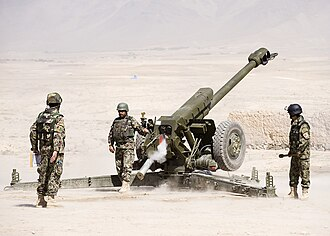
\includegraphics{../images/artyleria_holowana/m-46_1.jpg}
\caption{Armata M-46 130 mm}
\end{figure}

\subsection{Opis}\label{opis-28}

M-46 to radziecka armata polowa kalibru 130 mm opracowana przez Wasilija
Grabina i przyjęta do służby w 1954 roku. Jest jedną z dalekonośnych
armat polowych zimnej wojny --- zasięg do 27 490 m (z amunicją
aktywno-rakietową) czynił ją w latach 50.--80. jedną z najdłużej
strzelających armat konwencjonalnych na świecie. M-46 służyła w armiach
ponad 40 krajów, w tym Polski (do lat 90.), Chin, Syrii, Iranu i Indii
--- nadal jest aktywna w wielu siłach zbrojnych. Wymaga pełnego zaprzągu
holowniczego i obsługi 8--9 ludzi; waga ponad 8 ton czyni ją jedną z
cięższych armat holowanych.

\subsection{Dane techniczne}\label{dane-techniczne-28}

\begin{longtable}[]{@{}ll@{}}
\toprule\noalign{}
Parametr & Wartość \\
\midrule\noalign{}
\endhead
\bottomrule\noalign{}
\endlastfoot
Typ & Armata polowa dalekiego zasięgu \\
Kraj produkcji & ZSRR \\
Rok wprowadzenia & 1954 \\
Kaliber & 130 mm \\
Długość lufy & 6 895 mm (L/53) \\
Masa bojowa & 8 450 kg \\
Zasięg maks. & 27 490 m (aktywno-rakietowy) / 27 150 m (standardowy) \\
Kąt elevacji & −2,5° do +45° \\
Szybkostrzelność & 5--6 strz./min \\
Obsługa & 8--9 osób \\
\end{longtable}

\subsection{Charakterystyczne cechy
rozpoznawcze}\label{charakterystyczne-cechy-rozpoznawcze-28}

\begin{quote}
Jak odróżnić M-46 od D-20 i haubic 122 mm:
\end{quote}

\begin{itemize}
\tightlist
\item
  \textbf{Wyjątkowo długa lufa --- ponad 6,8 metra:} lufa M-46 ma 6,9 m
  długości, co daje proporcję długości do kalibrów L/53 --- bardzo
  charakterystyczna długa i cienka lufa; haubice 122/152 mm mają
  znacznie krótsze lufy
\item
  \textbf{Kaliber 130 mm --- unikalny w rosyjskiej artylerii:} M-46 jest
  jedyną powszechnie stosowaną armatą radziecką w kalibrze 130 mm; po
  wyglądzie nabojów (dłuższe, smuklejsze niż 152 mm i grubsze niż 122
  mm) można ją odróżnić
\item
  \textbf{Duży charakterystyczny hamulec wylotowy ``do przodu'':} M-46
  ma charakterystyczny wielokomorowy hamulec wylotowy na końcu długiej
  lufy --- widoczny z daleka jako ``rozszerzone'' zakończenie lufy
\item
  \textbf{Masywny lawet dwukolny z długimi ramionami odchylanymi:} lawet
  M-46 ma dwa duże stalowe koła i długie ramiona odchylane na boki w
  pozycji strzeleckiej (tworząc trójkąt stabilizujący) ---
  charakterystyczny rozkładany układ widoczny przy gotowości bojowej
\item
  \textbf{Ogromna masa --- przy transporcie widoczny 8-tonowy ciągnik
  artyleryjski:} M-46 jest holowana przez ciągnik AT-S lub KrAZ; ciężki
  ciągnik artyleryjski z tyłu to sygnał, że holowane działo jest ciężkim
  systemem --- nie lekką haubicą
\item
  \textbf{Wyraźnie większa i dłuższa niż D-30 czy 2S3:} przy
  bezpośrednim porównaniu M-46 jest dwa razy dłuższa od D-30 (długość
  lufy) i znacznie cięższa; proporcje całości są ``kanonierskie'' i
  monumentalne
\end{itemize}

\subsection{Ciekawostka}\label{ciekawostka-28}

\begin{quote}
M-46 miała nieoczekiwany wpływ na historię Bliskiego Wschodu: Egipt
używał jej do ostrzeliwania Izraela w wojnie 1973 roku (Jom Kippur), a
Iran i Irak strzelały do siebie tymi samymi armatami przez osiem lat w
wojnie 1980--1988. Chiny skopiowały M-46 jako typ 59-1 i sprzedawały go
wszystkim zainteresowanym --- sprawiając, że w wielu krajach strzelały
do siebie armatochy z identycznych sowieckich planów technicznych, tyle
że z różnymi oznakowaniami.
\end{quote}

\section{Haubica D-1}\label{haubica-d-1}

\subsubsection{D-1 Howitzer \textbar{} Д-1 (152-мм гаубица обр. 1943
г.)}\label{d-1-howitzer-ux434-1-152-ux43cux43c-ux433ux430ux443ux431ux438ux446ux430-ux43eux431ux440.-1943-ux433.}

\begin{center}\rule{0.5\linewidth}{0.5pt}\end{center}

\begin{figure}
\centering
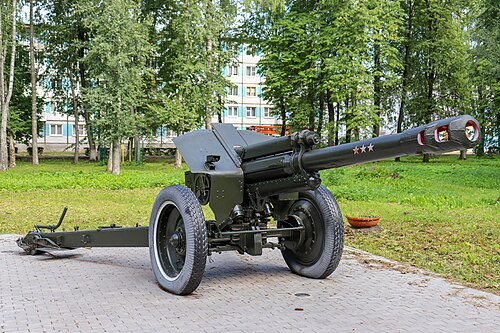
\includegraphics{../images/artyleria_holowana/d-1_1.jpg}
\caption{Haubica D-1 152 mm}
\end{figure}

\subsection{Opis}\label{opis-29}

D-1 to radziecka haubica kalibru 152 mm opracowana przez Fiodora
Pietrowa i przyjęta do służby w 1943 roku jako uproszczony następnik
starszej haubicy M-10. Zaprojektowana w środku II wojny światowej z
naciskiem na prostotę produkcji --- Sowieci potrzebowali ciężkiej
haubicy możliwej do masowej produkcji. D-1 zebrała doskonałe opinie na
froncie wschodnim i pozostała w służbie przez dekady. Kaliber 152 mm
daje jej znaczną siłę rażenia --- pocisk o masie 40 kg jest zdolny do
niszczenia ciężkich umocnień betonowych. Mimo bardzo podeszłego wieku
D-1 nadal pojawia się w konfliktach --- w tym na Ukrainie po 2022 roku,
gdzie oba strony wyciągnęły ją z magazynów.

\subsection{Dane techniczne}\label{dane-techniczne-29}

\begin{longtable}[]{@{}ll@{}}
\toprule\noalign{}
Parametr & Wartość \\
\midrule\noalign{}
\endhead
\bottomrule\noalign{}
\endlastfoot
Typ & Ciężka haubica holowana \\
Kraj produkcji & ZSRR \\
Rok wprowadzenia & 1943 \\
Kaliber & 152 mm \\
Długość lufy & 4 207 mm (L/27,7) \\
Masa bojowa & 3 600 kg \\
Zasięg maks. & 12 400 m \\
Kąt elevacji & −3° do +63,5° \\
Szybkostrzelność & 3--4 strz./min \\
Obsługa & 8 osób \\
\end{longtable}

\subsection{Charakterystyczne cechy
rozpoznawcze}\label{charakterystyczne-cechy-rozpoznawcze-29}

\begin{quote}
Jak odróżnić D-1 od D-20 i haubicy M-30 (122 mm):
\end{quote}

\begin{itemize}
\tightlist
\item
  \textbf{Krótka, gruba lufa 152 mm z wyraźnym hamulcem wylotowym:} D-1
  ma krótką lufę (tylko L/27,7) zakończoną dużym cylindrycznym
  dwukomorowym hamulcem wylotowym; w porównaniu z M-30 (122 mm) lufa
  jest grubsza i krótsza proporcjonalnie do kalibru
\item
  \textbf{Grube i szerokie koła gumowe na stalowych felgach:} D-1 ma
  charakterystyczne grube koła z gumowymi oponami --- inne niż
  archaiczne stalowe koła M-30 i nieco inne proporcje kół niż D-30;
  wyglądają ciężko i solidnie
\item
  \textbf{Lawet z dwoma składanymi ramionami --- ``płaski'' układ
  transportowy:} lawet D-1 jest prostą dwukolumną konstrukcją ze
  składanymi ramionami --- w transporcie układ jest płaski; to cecha
  wspólna z D-20, ale D-1 jest mniejsza i krótsza od D-20
\item
  \textbf{Mniejsza i lżejsza niż D-20 --- ale ten sam kaliber:} ktoś kto
  zna D-20 widzi, że D-1 jest wyraźnie krótsza (lufa L/27 vs L/38 w
  D-20) i lżejsza (3,6 t vs 5,7 t); jeśli kaliber trudno ocenić, to
  proporcje sylwetki wskazują na D-1
\item
  \textbf{Charakterystyczny kąt elevacji do 63,5° --- widoczna przy
  strzelaniu wysoko:} D-1 może strzelać bardzo stromo (max 63°), co jest
  cechą charakterystyczną haubic --- w pozycji maksymalnej elevacji lufa
  D-1 jest niemal pionowa
\item
  \textbf{Obsługa 8 osób --- widoczna przy pracy z ciężkimi pociskami
  152 mm:} pocisk D-1 waży 40--43 kg; jego ładowanie wymaga dwóch
  żołnierzy; przy obserwacji obsługi wyraźnie widać ciężką amunicję
  ładowaną ręcznie
\end{itemize}

\subsection{Ciekawostka}\label{ciekawostka-29}

\begin{quote}
D-1 została zaprojektowana w rekordowym tempie --- 18 dni od koncepcji
do gotowego prototypu w 1942 roku. Fiodor Pietrow, który wcześniej
zaprojektował M-30, po prostu założył lufę 152 mm na lawet M-30 ---
oszczędzając czas i pieniądze. To ``frankenstein-artyleria'' działała
tak dobrze, że Sowieci produkowali ją w ponad 2 800 egzemplarzy i do
dziś nie zastąpili jej w pełni. Na Ukrainie w 2022 roku D-1 pojawiła się
z obu stron frontu --- ponad 80-letnia broń strzelała nabojami z fabryk,
które zbudował Stalin.
\end{quote}

\section{Haubica-armata D-20}\label{haubica-armata-d-20}

\subsubsection{D-20 Gun-Howitzer \textbar{} Д-20 (152-мм
пушка-гаубица)}\label{d-20-gun-howitzer-ux434-20-152-ux43cux43c-ux43fux443ux448ux43aux430-ux433ux430ux443ux431ux438ux446ux430}

\begin{center}\rule{0.5\linewidth}{0.5pt}\end{center}

\begin{figure}
\centering
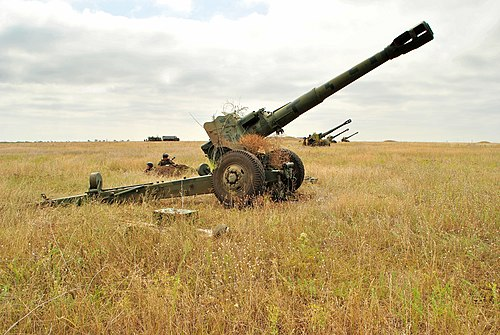
\includegraphics{../images/artyleria_holowana/d-20_1.jpg}
\caption{Haubica-armata D-20 152 mm}
\end{figure}

\subsection{Opis}\label{opis-30}

D-20 to radziecka haubica-armata kalibru 152 mm opracowana przez Fiodora
Pietrowa i przyjęta do służby w 1955 roku. Łączy w sobie właściwości
haubicy (wysoka elevacja, stromy tor pocisku) i armaty (długa lufa, duża
prędkość wylotowa, płaski tor) --- stąd określenie ``haubica-armata''.
Używa tej samej amunicji co samobieżna 2S3 Akacja, co upraszcza
logistykę. D-20 przez dekady była standardową ciężką artylerią dywizyjną
krajów Układu Warszawskiego --- służyła w Polsce, NRD, Czechosłowacji i
innych armiach. Nadal używana przez armię rosyjską (głównie rezerwy i
magazyny) i wiele armii świata.

\subsection{Dane techniczne}\label{dane-techniczne-30}

\begin{longtable}[]{@{}ll@{}}
\toprule\noalign{}
Parametr & Wartość \\
\midrule\noalign{}
\endhead
\bottomrule\noalign{}
\endlastfoot
Typ & Haubica-armata holowana \\
Kraj produkcji & ZSRR \\
Rok wprowadzenia & 1955 \\
Kaliber & 152 mm \\
Długość lufy & 5 195 mm (L/34,2) \\
Masa bojowa & 5 700 kg \\
Zasięg maks. & 17 400 m (standardowy) / 24 000 m (aktywno-rakietowy) \\
Kąt elevacji & −5° do +65° \\
Szybkostrzelność & 5--6 strz./min \\
Obsługa & 8 osób \\
\end{longtable}

\subsection{Charakterystyczne cechy
rozpoznawcze}\label{charakterystyczne-cechy-rozpoznawcze-30}

\begin{quote}
Jak odróżnić D-20 od D-1 i haubicy D-30 (122 mm):
\end{quote}

\begin{itemize}
\tightlist
\item
  \textbf{Długa lufa 152 mm z charakterystycznym wielokomorowym hamulcem
  wylotowym:} D-20 ma lufę wyraźnie dłuższą niż D-1 (L/34 vs L/27)
  zakończoną charakterystycznym podwójnym lub wielokomorowym hamulcem
  wylotowym --- ``łatka'' na końcu lufy jest wizualnie bardziej
  rozbudowana niż w D-1
\item
  \textbf{Dwa składane ramiona lawetu w kształcie litery V:} w pozycji
  strzeleckiej D-20 ma dwa ramiona odchylane na boki tworząc szerokie
  ``V'' --- daje to stabilność przy dużym odrzucie; D-30 ma trzy ramiona
  układające się w gwiazdę; D-1 ma węższe ``V''
\item
  \textbf{Masywne stalowo-gumowe koła z charakterystycznymi felgami:}
  koła D-20 są duże (ok. 1 m średnicy), solidne, z gumowymi oponami;
  wyraźnie masywniejsze niż koła D-30 (122 mm)
\item
  \textbf{Wyraźnie cięższa i dłuższa od D-30 --- widoczna różnica
  gabarytów:} D-20 waży 5,7 t a D-30 waży 3,2 t; przy porównaniu obie są
  kołowe i haubiczne, ale D-20 jest znacznie większa; długość lawetu z
  lufą D-20 jest o ok. 1,5 m dłuższa
\item
  \textbf{Lufa opuszczona w transport poziomo ponad lawet:} w
  konfiguracji transportowej lufa D-20 jest pozioma, skierowana do
  przodu nad ramionami lawetu; charakterystyczna długa lufa nadaje
  sylwetce ``strzałkowy'' kształt przy holowaniu
\item
  \textbf{Ten sam kaliber i amunicja co 2S3 Akacja:} D-20 i samobieżna
  2S3 używają tych samych nabojów 152 mm; przy obserwacji amunicji ---
  te same duże żółte pociski
\end{itemize}

\subsection{Ciekawostka}\label{ciekawostka-30}

\begin{quote}
D-20 była numerem jeden w polskiej artylerii dywizyjnej przez całą zimną
wojnę --- Polska miała ponad 500 sztuk D-20. Kiedy Polska wycofała D-20
ze służby i przeszła na NATO-wskie haubice 155 mm, część egzemplarzy
trafiła do muzeów, część sprzedano, a część --- co kontrowersyjne ---
wróciła przez eksport do Afryki i Bliskiego Wschodu. W 2022 roku Polska
przekazała część swojego sprzętu Ukrainie --- i D-20, podobnie jak 2S1,
stanęły po ukraińskiej stronie frontu.
\end{quote}

\section{Haubica 2A65 Msta-B}\label{haubica-2a65-msta-b}

\subsubsection{2A65 Msta-B Howitzer \textbar{} 2А65
«Мста-Б»}\label{a65-msta-b-howitzer-2ux43065-ux43cux441ux442ux430-ux431}

\begin{center}\rule{0.5\linewidth}{0.5pt}\end{center}

\begin{figure}
\centering
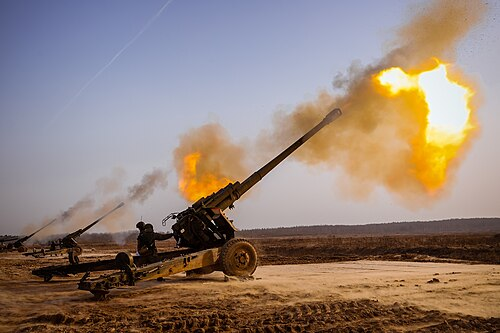
\includegraphics{../images/artyleria_holowana/msta-b_1.jpg}
\caption{Haubica 2A65 Msta-B 152 mm}
\end{figure}

\subsection{Opis}\label{opis-31}

2A65 Msta-B to rosyjska holowana haubica kalibru 152 mm opracowana w
latach 80. i przyjęta do służby w 1987 roku jako holowana wersja
samobieżnej 2S19 Msta-S. Używa tych samych luf i amunicji co 2S19 --- co
upraszcza logistykę i szkolenie. Msta-B ma zasięg do 24 700 m (pocisk
standardowy) i do 30 000 m z amunicją aktywno-rakietową, w tym z
precyzyjnym pociskiem Krasnopol naprowadzanym laserowo. Jest to jedna z
najnowocześniejszych holowanych haubic w służbie rosyjskiej --- łączy
klasyczną prostotę holowanego działa z możliwościami ogniowymi
samobieżnego systemu Msta-S. Szeroko stosowana w wojnie na Ukrainie po
obu stronach konfliktu.

\subsection{Dane techniczne}\label{dane-techniczne-31}

\begin{longtable}[]{@{}ll@{}}
\toprule\noalign{}
Parametr & Wartość \\
\midrule\noalign{}
\endhead
\bottomrule\noalign{}
\endlastfoot
Typ & Holowana haubica ciężka \\
Kraj produkcji & Rosja \\
Rok wprowadzenia & 1987 \\
Kaliber & 152 mm \\
Długość lufy & 7 200 mm (L/47,4) \\
Masa bojowa & 7 000 kg \\
Zasięg maks. & 24 700 m (standardowy) / 30 000 m (aktywno-rakietowy) \\
Kąt elevacji & −3° do +70° \\
Szybkostrzelność & 6--8 strz./min \\
Obsługa & 8 osób \\
\end{longtable}

\subsection{Charakterystyczne cechy
rozpoznawcze}\label{charakterystyczne-cechy-rozpoznawcze-31}

\begin{quote}
Jak odróżnić Msta-B od D-20 i holowanych haubic NATO:
\end{quote}

\begin{itemize}
\tightlist
\item
  \textbf{Bardzo długa lufa 152 mm --- najdłuższa wśród holowanych
  haubic rosyjskich:} lufa Msta-B ma 7,2 m (L/47), wyraźnie dłuższa od
  D-20 (5,2 m) i D-1 (4,2 m); ta proporcja czyni Mstę-B
  charakterystyczną --- ``wąska i długa''
\item
  \textbf{Charakterystyczny wielokomorowy hamulec wylotowy na bardzo
  długiej lufie:} hamulec wylotowy Msta-B jest duży i wielosegmentowy,
  osadzony na końcu wyjątkowo długiej lufy --- kombinacja długości i
  dużego hamulca jest kluczowym wyróżnikiem wizualnym
\item
  \textbf{Dwa szerokie ramiona lawetu w konfiguracji ``V'' --- podobne
  do D-20 ale masywniejsze:} Msta-B ma klasyczne dwa odchylane ramiona,
  ale cały lawet jest wyraźnie masywniejszy i nowocześ­niejszy niż D-20;
  bardziej kanciaste kształty elementów metalowych
\item
  \textbf{Platforma kołowa z hydraulicznym układem poziomowania:} Msta-B
  ma mały hydrauliczny układ stabilizowania platformy przed strzelaniem
  --- charakterystyczne cylindry hydrauliczne widoczne przy nogach
  lawetu; starsze D-20 i D-1 nie mają hydrauliki
\item
  \textbf{Osłona balistyczna obsługi (tarcza) mała i geometryczna:}
  Msta-B ma skromną metalową tarczę chroniącą obsługę; jej geometryczny,
  kanciasty kształt różni się od zaokrąglonych tarcz starszych dział
  radzieckich
\item
  \textbf{Ta sama amunicja co 2S19 Msta-S i pociski Krasnopol:}
  rozpoznanie po amunicji --- Msta-B używa nowoczesnych pocisków 152 mm,
  w tym charakterystycznych pocisków Krasnopol z półprzezroczystymi
  żółto-brązowymi noskami laserowymi
\end{itemize}

\subsection{Ciekawostka}\label{ciekawostka-31}

\begin{quote}
Msta-B jest wyjątkowym przypadkiem: holowane działo zaprojektowane po
samobieżnym. Zwykle holowane systemy poprzedzają samobieżne --- Msta-B
jest odwrotnie, bo projektanci wzięli gotową lufę 2S19 i umieścili ją na
kołowym lawecie. Efektem jest holowana haubica z możliwościami ogniowymi
dorównującymi wielu samobieżnym systemom NATO. Na Ukrainie Msta-B
pojawiła się po obu stronach frontu --- ukraińskie wojska zdobywały
rosyjskie egzemplarze i natychmiast je używały, ponieważ mają te same
lufy co rosyjskie, a amunicja jest zamienna.
\end{quote}

\section{Armata 2A36 Giacynt-B}\label{armata-2a36-giacynt-b}

\subsubsection{2A36 Giatsint-B Field Gun \textbar{} 2А36
«Гиацинт-Б»}\label{a36-giatsint-b-field-gun-2ux43036-ux433ux438ux430ux446ux438ux43dux442-ux431}

\begin{center}\rule{0.5\linewidth}{0.5pt}\end{center}

\begin{figure}
\centering
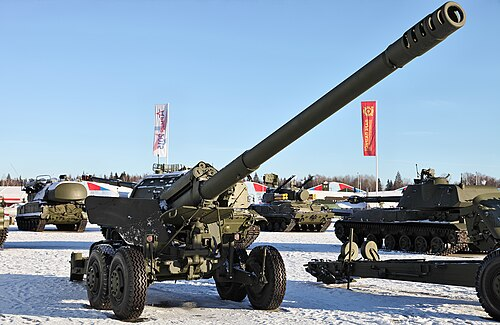
\includegraphics{../images/artyleria_holowana/giatsint-b_1.jpg}
\caption{Armata 2A36 Giacynt-B 152 mm}
\end{figure}

\subsection{Opis}\label{opis-32}

2A36 Giacynt-B (Гиацинт --- Hiacynt) to radziecka potężna armata polowa
kalibru 152 mm opracowana w latach 70. i przyjęta do służby w 1976 roku.
Wyróżnia się wyjątkowo długą lufą (L/54) zapewniającą zasięg do 27 200 m
standardowym pociskiem i do 40 000 m amunicją aktywno-rakietową --- co
czyni ją jedną z najdłużej strzelających holowanych armat na świecie.
Giacynt-B jest holowaną wersją samobieżnej 2S5 Giacynt-S i używa tej
samej amunicji. Ze względu na masę ponad 9 ton wymaga ciągnika
artyleryjskiego KrAZ lub AT-T. Stosowana jako działo kontrbateryjne i
rażące cele w głębokości obrony przeciwnika.

\subsection{Dane techniczne}\label{dane-techniczne-32}

\begin{longtable}[]{@{}ll@{}}
\toprule\noalign{}
Parametr & Wartość \\
\midrule\noalign{}
\endhead
\bottomrule\noalign{}
\endlastfoot
Typ & Armata polowa ciężka \\
Kraj produkcji & ZSRR / Rosja \\
Rok wprowadzenia & 1976 \\
Kaliber & 152 mm \\
Długość lufy & 8 197 mm (L/54) \\
Masa bojowa & 9 800 kg \\
Zasięg maks. & 27 200 m (standardowy) / 40 000 m (aktywno-rakietowy) \\
Kąt elevacji & −2° do +57° \\
Szybkostrzelność & 5--6 strz./min \\
Obsługa & 8 osób \\
\end{longtable}

\subsection{Charakterystyczne cechy
rozpoznawcze}\label{charakterystyczne-cechy-rozpoznawcze-32}

\begin{quote}
Jak odróżnić Giacynt-B od Msta-B i D-20:
\end{quote}

\begin{itemize}
\tightlist
\item
  \textbf{Najdłuższa lufa spośród wszystkich holowanych armat 152 mm ---
  ponad 8 metrów:} lufa 8,2 m czyni Giacynt-B wyjątkową --- jest o metr
  dłuższa od Msta-B i o 3 metry dłuższa od D-20; przy transporcie lufa
  wystaje daleko przed ciągnik lub za niego
\item
  \textbf{Duży, charakterystyczny hamulec wylotowy w kształcie
  ``kuli'':} Giacynt-B ma charakterystyczny kulisto-cylindryczny hamulec
  wylotowy na końcu bardzo długiej lufy --- inny kształt niż
  wielosegmentowe hamulce Msta-B; ten ``kulowy'' zakończenie jest
  kluczowym identyfikatorem wizualnym
\item
  \textbf{Masywny lawet z szerokim rozstawem kół i dużymi ogumieniami:}
  Giacynt-B jest wyraźnie cięższy od Msta-B (9,8 t vs 7 t); lawet jest
  masywniejszy, z większymi kołami; ciężarówki holujące Giacynt-B to
  wielotonowe ciągniki, nie lekkie pojazdy
\item
  \textbf{Brak osłony (tarczy) obsługi --- otwarta platforma
  strzelecka:} Giacynt-B nie ma tarczy balistycznej chroniącej obsługę
  --- to ``gołe'' działo artyleryjskie; Msta-B i D-20 mają przynajmniej
  minimalną osłonę
\item
  \textbf{Wyraźnie ``armatni'' wygląd --- mniejszy kąt elevacji niż
  haubice:} armata Giacynt-B ma mniejszy kąt elevacji (max 57°) niż
  haubice Msta-B (70°) i D-20 (65°) --- przy strzelaniu lufa jest
  bardziej pozioma, jak przystało armacie
\item
  \textbf{Holowanie wymaga ciągnika artyleryjskiego klasy KrAZ lub
  AT-T:} masa 9,8 t wymaga ciągnika gąsienicowego lub ciężkiego
  kołowego; przy kolumnie marszowej widoczny ciągnik artyleryjski za
  Giacyntem jest sam w sobie sygnałem, że holowane działo jest wyjątkowo
  ciężkie
\end{itemize}

\subsection{Ciekawostka}\label{ciekawostka-32}

\begin{quote}
Giacynt-B był jedną z odpowiedzi Sowietów na zachodnie działa
kontrbateryjne z lat 70. --- w szczególności na amerykański M198 155 mm
i jego zasięg 22 km. Sowieci chcieli coś, co ``przeleci nad'' M198 i
uderzy w stanowiska ogniowe, zanim M198 zdąży odpowiedzieć. Giacynt-B ze
swoimi 27 km zasięgu (i 40 km z amunicją rakietową) spełniał to zadanie
z nadwyżką. W wojnie na Ukrainie Giacynt-B pojawił się po stronie
rosyjskiej jako broń kontrbateryjna --- celując w ukraińskie haubice
M777 i Krab.
\end{quote}

\section{Armata przeciwpancerna MT-12
Rapira}\label{armata-przeciwpancerna-mt-12-rapira}

\subsubsection{MT-12 Rapira 100mm Anti-Tank Gun \textbar{} МТ-12
«Рапира»}\label{mt-12-rapira-100mm-anti-tank-gun-ux43cux442-12-ux440ux430ux43fux438ux440ux430}

\begin{figure}
\centering
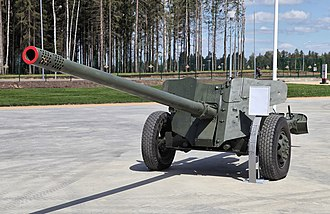
\includegraphics{../images/artyleria_holowana/mt-12_1.jpg}
\caption{MT-12 Rapira --- ekspozycja w Parku Patriot}
\end{figure}

\begin{center}\rule{0.5\linewidth}{0.5pt}\end{center}

\subsection{Opis}\label{opis-33}

MT-12 Rapira (ros. «Рапира» --- rapier) to radziecka 100 mm armata
przeciwpancerna gładkolufowa, wprowadzona do służby w 1970 roku jako
unowocześnienie armaty T-12. Przeznaczona jest do bezpośredniego
zwalczania pojazdów opancerzonych, fortyfikacji i schronów. Może
strzelać pociskami APFSDS, HEAT i HE, a także pociskami kierowanymi
9M117 Bastion (ppk odpalany przez lufę). Choć MT-12 nie może przebić
frontowego pancerza nowoczesnych czołgów głównych, jest wciąż używana do
zwalczania BWP, transporterów i czołgów starszych generacji, a także
jako działo wsparcia ogniowego. W wojnie w Ukrainie jednostki OT stosują
ją intensywnie.

\subsection{Dane techniczne}\label{dane-techniczne-33}

\begin{longtable}[]{@{}ll@{}}
\toprule\noalign{}
Parametr & Wartość \\
\midrule\noalign{}
\endhead
\bottomrule\noalign{}
\endlastfoot
Typ & Armata przeciwpancerna holowana 100 mm \\
Kraj produkcji & ZSRR \\
Rok wprowadzenia & 1970 \\
Kaliber & 100 mm (gładkolufowa) \\
Masa bojowa & 3 050 kg \\
Zasięg (bezpośredni) & 3 000 m \\
Zasięg (pośredni) & 8 200 m \\
Przenikanie pancerza & 390--450 mm (APFSDS) \\
Ppk 9M117 Bastion & do 5 000 m, 650 mm za ERA \\
Obsługa & 7 osób \\
\end{longtable}

\subsection{Charakterystyczne cechy
rozpoznawcze}\label{charakterystyczne-cechy-rozpoznawcze-33}

\begin{quote}
Jak odróżnić MT-12 od D-30 i innych dział holowanych:
\end{quote}

\begin{itemize}
\tightlist
\item
  \textbf{Bardzo długa, cienka lufa gładkolufowa bez hamulca
  wylotowego:} MT-12 ma jedną z najdłuższych i najsmuklejszych luf wśród
  holowanych dział tego kalibru --- brak hamulca wylotowego
  (gładkolufowa) to charakterystyczny element
\item
  \textbf{Dwójnożne łoże rozchylane (nie trójnóg jak D-30):} łoże MT-12
  rozkłada się w dwie nogi --- nie trzy jak D-30; w pozycji bojowej
  wygląda jak odwrócona litera ``V''
\item
  \textbf{Tarcza pancerna z dużym wycięciem na lufę:} z przodu MT-12
  widoczna jest duża pionowa tarcza ochronna z centralnym wycięciem
  przez które przechodzi lufa --- tarcza jest wyżej niż w D-30
\item
  \textbf{Duże koła ze stalowymi obręczami (bez opon) lub z oponami:}
  MT-12 ma charakterystyczne duże koła --- część egzemplarzy ma gumowe
  opony terenowe, część starszych ma stalowe obręcze
\item
  \textbf{Profil ``bardzo niska armata z długą lufą'':} sylwetka MT-12 z
  boku to bardzo niska konstrukcja z nieproporcjonalnie długą, cienką
  lufą --- specyficzny profil różniący się od haubic
\item
  \textbf{Lufa bez osłony termicznej i bez kompensatora:} gładka lufa
  bez żadnych dodatków na końcu to główny identyfikator; porównaj z D-30
  (hamulec wylotowy) czy M-46 (hamulec + kompensator)
\end{itemize}

\subsection{Ciekawostka}\label{ciekawostka-33}

\begin{quote}
MT-12 jest jedną z niewielu armat holowanych zaprojektowanych do
strzelania pociskami kierowanymi przez lufę --- system 9M117 Bastion
pozwala wystrzelić ppk z lufy działa, prowadząc go laserowo do celu.
Oznacza to, że stara armata holowana może trafić w czołg z odległości 5
km z pierwszego strzału --- coś niemożliwego dla standardowej amunicji
tej armaty. To rozwiązanie przedłuża użyteczność MT-12 o kolejne dekady
mimo rosnącej grubości pancerzy.
\end{quote}

\section{Automatyczny moździerz 2B9
Wasilek}\label{automatyczny-moux17adzierz-2b9-wasilek}

\subsubsection{2B9 Vasilek Automatic Mortar \textbar{} 2Б9
«Василёк»}\label{b9-vasilek-automatic-mortar-2ux4319-ux432ux430ux441ux438ux43bux451ux43a}

\begin{center}\rule{0.5\linewidth}{0.5pt}\end{center}

\begin{figure}
\centering
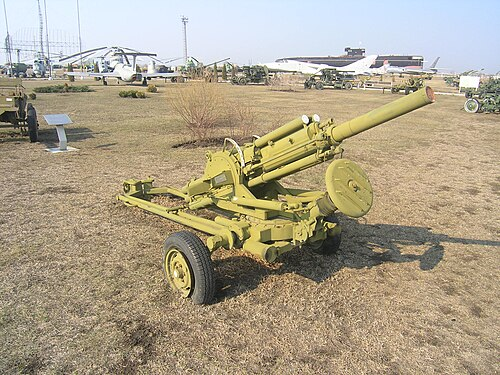
\includegraphics{../images/artyleria_holowana/vasilek_1.jpg}
\caption{Moździerz automatyczny 2B9 Wasilek}
\end{figure}

\subsection{Opis}\label{opis-34}

2B9 Wasilek (Василёк --- Chaber) to radziecka automatyczna
armata-moździerz kalibru 82 mm opracowana w 1967 roku i przyjęta do
służby w 1970 roku. Wyróżnia się wśród moździerzy możliwością
prowadzenia ognia automatycznego --- przy użyciu taśmowego podawania
amunicji Wasilek strzela z szybkostrzelnością do 170 nabojów na minutę
(serie po 4 naboje), co jest nieosiągalne dla klasycznych moździerzy.
Może strzelać zarówno po standardowej trajektorii moździerzowej (wyrzut
w górę), jak i napiętym lotem bezpośrednim jak haubica --- co daje dużą
elastyczność taktyczną. Jest ciągnięty przez lekki pojazd lub montowany
na różnych platformach. Stosowany przez wiele armii byłego ZSRR i krajów
Bliskiego Wschodu.

\subsection{Dane techniczne}\label{dane-techniczne-34}

\begin{longtable}[]{@{}
  >{\raggedright\arraybackslash}p{(\columnwidth - 2\tabcolsep) * \real{0.5263}}
  >{\raggedright\arraybackslash}p{(\columnwidth - 2\tabcolsep) * \real{0.4737}}@{}}
\toprule\noalign{}
\begin{minipage}[b]{\linewidth}\raggedright
Parametr
\end{minipage} & \begin{minipage}[b]{\linewidth}\raggedright
Wartość
\end{minipage} \\
\midrule\noalign{}
\endhead
\bottomrule\noalign{}
\endlastfoot
Typ & Automatyczny moździerz / armata-moździerz \\
Kraj produkcji & ZSRR / Rosja \\
Rok wprowadzenia & 1970 \\
Kaliber & 82 mm \\
Długość lufy & 1 200 mm \\
Masa bojowa & 632 kg \\
Zasięg maks. & 4 270 m \\
Zasięg min. & 800 m \\
Szybkostrzelność & do 170 strz./min (automatycznie), 1--3 strz./min
(ręcznie) \\
Obsługa & 4 osoby \\
\end{longtable}

\subsection{Charakterystyczne cechy
rozpoznawcze}\label{charakterystyczne-cechy-rozpoznawcze-34}

\begin{quote}
Jak odróżnić 2B9 Wasilek od klasycznych moździerzy i lekkich armat:
\end{quote}

\begin{itemize}
\tightlist
\item
  \textbf{Lufa ustawiona poziomo lub pod małym kątem --- nie pionowo jak
  moździerz:} Wasilek w trybie bezpośrednim strzela płaskim torem;
  wizualnie wygląda jak mała armata lub działo, nie jak typowy moździerz
  stojący prawie pionowo --- to kluczowa cecha odróżniająca
\item
  \textbf{Podajnik taśmowy z boku lufy:} charakterystyczny poziomy
  podajnik z taśmą nabojów biegnący prostopadle do lufy --- widoczny
  element odróżniający Wasilka od wszystkich innych moździerzy; żaden
  klasyczny moździerz nie ma taśmowego podajnika
\item
  \textbf{Czterokołowy lawet artyleryjski (nie podstawa płytowa):}
  Wasilek jest montowany na kołowym lawecie artyleryjskim ciągnionym
  przez pojazd --- klasyczne moździerze stoją na stalowej płycie bazowej
  wkopanej w ziemię; Wasilek można przytransportować szybko bez
  rozkładania
\item
  \textbf{Układ lufy podobny do małej haubicy lub granatnika:} proporcje
  są artyleryjskie, nie moździerzowe --- lufa jest stosunkowo długa (120
  cm), a bryła przypomina miniaturową armatę przeciwpancerną bardziej
  niż moździerz
\item
  \textbf{Mała, kompaktowa platforma --- wyraźnie lżejsza niż działa
  artylerii:} całość waży 632 kg i jest wyraźnie mniejsza od haubic 122
  mm; można ją łatwo odróżnić od D-30 czy 2S1 po miniaturowych
  rozmiarach
\item
  \textbf{Amunicja 82 mm w taśmach po 4 sztuki:} charakterystyczne
  ``taśmy'' z czterema nabojami używane do automatycznego ładowania ---
  widoczne przy obsłudze i w transporterach amunicji; żaden inny system
  moździerzowy nie używa taśmowania
\end{itemize}

\subsection{Ciekawostka}\label{ciekawostka-34}

\begin{quote}
Wasilek był używany przez obie strony w wojnie afgańskiej. Radzieccy
żołnierze szczególnie cenili go za możliwość prowadzenia ognia
automatycznego --- mówili, że ``Wasilek zamienia moździerz w karabin
maszynowy''. Mudżahedini zdobywali Wasilki i używali ich przeciwko
Sowietom --- co było jednym z paradoksów tej wojny. Broń miała też wadę:
automatyczne ładowanie powodowało szybkie przegrzanie lufy, przez co
serie dłuższe niż 40 nabojów wymagały ochłodzenia wodą lub przerwy; w
suchym klimacie Afganistanu było to poważnym problemem.
\end{quote}

\section{Moździerz 2B14 Podnos}\label{moux17adzierz-2b14-podnos}

\subsubsection{2B14 Podnos Mortar \textbar{} 2Б14
«Поднос»}\label{b14-podnos-mortar-2ux43114-ux43fux43eux434ux43dux43eux441}

\begin{center}\rule{0.5\linewidth}{0.5pt}\end{center}

\begin{figure}
\centering
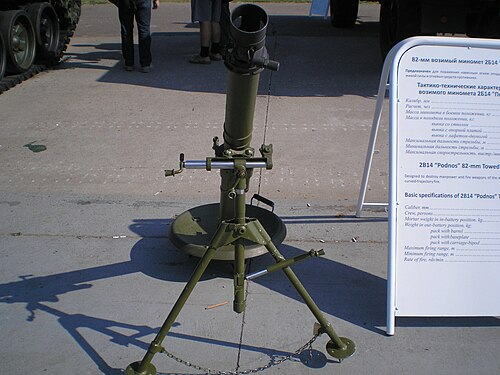
\includegraphics{../images/artyleria_holowana/podnos_1.jpg}
\caption{Moździerz piechoty 2B14 Podnos}
\end{figure}

\subsection{Opis}\label{opis-35}

2B14 Podnos (Поднос --- Taca) to radziecko-rosyjski lekki moździerz
piechoty kalibru 82 mm opracowany w latach 70. i przyjęty do służby w
1983 roku jako zastępnik przestarzałego moździerza BM-37. Wyróżnia się
bardzo prostą, lekką i wytrzymałą konstrukcją --- całość waży zaledwie
42 kg, co pozwala na transport przez trzyosobową drużynę (lufa, płyta
bazowa i trójnóg w trzech osobnych częściach). Podnos może strzelać bez
rozkładania trójnogu bezpośrednio z płyty bazowej, co przyspiesza
gotowość bojową. Jest podstawowym moździerzem szczebla pluton-kompania w
armii rosyjskiej i był szeroko stosowany w Afganistanie, Czeczenii i na
Ukrainie.

\subsection{Dane techniczne}\label{dane-techniczne-35}

\begin{longtable}[]{@{}ll@{}}
\toprule\noalign{}
Parametr & Wartość \\
\midrule\noalign{}
\endhead
\bottomrule\noalign{}
\endlastfoot
Typ & Lekki moździerz piechoty \\
Kraj produkcji & ZSRR / Rosja \\
Rok wprowadzenia & 1983 \\
Kaliber & 82 mm \\
Długość lufy & 1 220 mm \\
Masa bojowa & 42 kg (całość) \\
Zasięg maks. & 4 000 m \\
Zasięg min. & 85 m \\
Szybkostrzelność & 20--25 strz./min \\
Obsługa & 3 osoby \\
\end{longtable}

\subsection{Charakterystyczne cechy
rozpoznawcze}\label{charakterystyczne-cechy-rozpoznawcze-35}

\begin{quote}
Jak odróżnić 2B14 Podnos od moździerza PM-38/BM-37 i 2B9 Wasilek:
\end{quote}

\begin{itemize}
\tightlist
\item
  \textbf{Klasyczna pionowa lufa moździerzowa --- wyraźnie prosta i
  długa:} Podnos jest typowym moździerzem klasycznym --- lufa stoi
  prawie pionowo (60--85°); żadnych poziomych luf, taśmowników ani kół
  artyleryjskich jak w Wasilku
\item
  \textbf{Okrągła kwadratowa lub prostokątna płyta bazowa stalowa:}
  płyta bazowa Podnosu jest prostokątna z charakterystycznym wzorem
  usztywnień; płyta BM-37 jest okrągła --- różnica kształtu płyty jest
  dobrym wyróżnikiem
\item
  \textbf{Lekki prosty trójnóg z mechanizmem kątowania:} trójnóg Podnosu
  jest uproszczony i wyraźnie lżejszy niż starszych moździerzy; całość
  wygląda nowocześ­niej i bardziej kanciasty niż BM-37
\item
  \textbf{Brak kółek transportowych (w odróżnieniu od Wasilka):} Podnos
  nie ma kół ani lawetu --- jest rozkładany na ziemi i noszony w
  częściach; Wasilek ma kołowy lawet artyleryjski; ta różnica
  natychmiast odróżnia oba systemy
\item
  \textbf{Mały rozmiar całości --- kompaktowość:} złożony Podnos mieści
  się w plecakach trzech żołnierzy; przy rozłożonym moździerzu widać, że
  jest wyraźnie mniejszy i prostszy niż haubice czy samobieżne działa
  artylerii
\item
  \textbf{Amunicja 82 mm wkładana od góry lufy --- ładowanie gwintowe:}
  żołnierz ładuje nabój wkładając go od góry do lufy --- standardowy
  sposób ładowania klasycznych moździerzy; Wasilek natomiast ładuje się
  automatycznie z taśmy z boku
\end{itemize}

\subsection{Ciekawostka}\label{ciekawostka-35}

\begin{quote}
Podnos jest tak prosty i tani, że produkowany jest w Rosji bez zmian od
1983 roku --- co jest rekordem jak na nowoczesną broń. Ukraina i Rosja
używają identycznych Podnosów po obu stronach linii frontu w wojnie
2022--; bywa, że zdobyte przez jedną ze stron pociski idealnie pasują do
moździerzy przeciwnika. Żołnierze rosyjscy mówią, że Podnos ``nie psuje
się nigdy'' --- i dodają, że to jedyna broń w piechurze, o której
serwisie zapomina się zupełnie.
\end{quote}

\section{Ciężki moździerz 2S12
Sani}\label{ciux119ux17cki-moux17adzierz-2s12-sani}

\subsubsection{2S12 Sani Heavy Mortar \textbar{} 2С12
«Сани»}\label{s12-sani-heavy-mortar-2ux44112-ux441ux430ux43dux438}

\begin{center}\rule{0.5\linewidth}{0.5pt}\end{center}

\begin{figure}
\centering
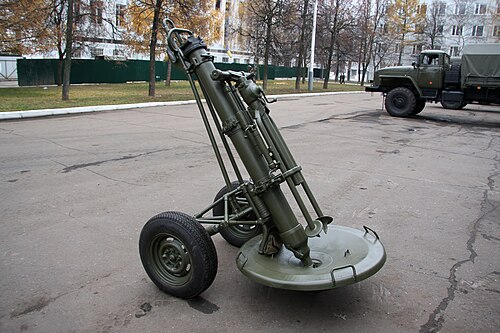
\includegraphics{../images/artyleria_holowana/sani_1.jpg}
\caption{Ciężki moździerz 2S12 Sani}
\end{figure}

\subsection{Opis}\label{opis-36}

2S12 Sani (Сани --- Sanie) to radziecki ciężki moździerz piechoty
kalibru 120 mm opracowany w latach 70. jako przenośny system o zasięgu i
sile rażenia pośrednim między lekkimi moździerzami 82 mm a artylerią
polową. Sani waży 210 kg i jest holowany na dwukołowym lawecie przez
lekki pojazd (UAZ-469, GAZ-66), ale może też być rozkładany do pozycji
strzeleckiej bezpośrednio na ziemi. Pocisk 120 mm Sani ma znacznie
większą siłę rażenia niż 82 mm moździerze Podnos i Wasilek --- może
niszczyć lekkie pojazdy opancerzone i umocnienia polowe. Jest
standardowym moździerzem szczebla batalionu w armii rosyjskiej.

\subsection{Dane techniczne}\label{dane-techniczne-36}

\begin{longtable}[]{@{}ll@{}}
\toprule\noalign{}
Parametr & Wartość \\
\midrule\noalign{}
\endhead
\bottomrule\noalign{}
\endlastfoot
Typ & Ciężki moździerz holowany \\
Kraj produkcji & ZSRR / Rosja \\
Rok wprowadzenia & 1981 \\
Kaliber & 120 mm \\
Długość lufy & 1 854 mm \\
Masa bojowa & 210 kg \\
Zasięg maks. & 7 100 m \\
Zasięg min. & 480 m \\
Szybkostrzelność & 12--15 strz./min \\
Obsługa & 5 osób \\
\end{longtable}

\subsection{Charakterystyczne cechy
rozpoznawcze}\label{charakterystyczne-cechy-rozpoznawcze-36}

\begin{quote}
Jak odróżnić 2S12 Sani od 2B14 Podnos i moździerza M-120:
\end{quote}

\begin{itemize}
\tightlist
\item
  \textbf{Znacznie większa i cięższa konstrukcja niż 82 mm moździerze:}
  Sani waży 210 kg i ma lufę niemal 2 metry --- wizualnie jest wyraźnie
  większy od Podnosu; przy bezpośrednim porównaniu różnica kalibrów 82
  vs 120 mm jest oczywista
\item
  \textbf{Dwukołowy lawet transportowy:} Sani jest holowany na dwóch
  kółkach --- kiedy stoi w pozycji bojowej, kółka są uniesione lub
  zdjęte; ten charakterystyczny lawet odróżnia Sani od prostego Podnosu,
  który nie ma kół
\item
  \textbf{Duża okrągła płyta bazowa ze wzorem radialnym:} płyta bazowa
  Sani 120 mm jest większa i cięższa od płyty Podnosu; charakterystyczny
  okrągły lub wielokątny kształt z grubszymi żebrami wzmacniającymi
\item
  \textbf{Lufa z zewnętrznym pierścieniem komory nabojowej:} Sani ma
  charakterystyczny ``garb'' na lufie przy komorze nabojowej --- grubszy
  odcinek w dolnej części lufy --- widoczny przy bliższym ogladaniu,
  inny od gładkiej lufy Podnosu
\item
  \textbf{Obsługa 5-osobowa --- znacznie więcej niż 3-osobowy Podnos:}
  do obsługi Sani potrzeba 5 żołnierzy ze względu na ciężkie naboje 120
  mm; operacja załadowania wymaga dwóch ludzi; to widoczne podczas
  strzelania
\item
  \textbf{Transport przez pojazd --- holowany, nie noszony:} Sani nie
  jest noszony w plecakach; do jego transportu konieczny jest pojazd
  (UAZ lub ciężarówka); przy rozbiórce i złożeniu na ziemi zajmuje
  znacznie więcej miejsca niż Podnos
\end{itemize}

\subsection{Ciekawostka}\label{ciekawostka-36}

\begin{quote}
2S12 Sani zyskał nieoczekiwanie dużą popularność wśród rosyjskich
artylerzystów w wojnach czeczeńskich --- bo naboje 120 mm mogły niszczyć
budynki murowane, których nie ``przebijał'' moździerz 82 mm. Dowódcy
batalionów mówili, że Sani to ``artyleria dla piechoty'': lżejszy od
haubicy, łatwiejszy do przebiegi w górach niż samobieżna artyleria, a
siłą ognia porównywalny z lekkimi działami. Paradoksalnie, po wojnie
afgańskiej część Sanich trafiła do mudżahedinów --- którzy oceniali je
wyżej niż zdobyte moździerze zachodnie.
\end{quote}

\section{ZU-23-2 --- holowane działko przeciwlotnicze 23
mm}\label{zu-23-2-holowane-dziaux142ko-przeciwlotnicze-23-mm}

\subsubsection{ZU-23-2 Anti-Aircraft Gun \textbar{}
ЗУ-23-2}\label{zu-23-2-anti-aircraft-gun-ux437ux443-23-2}

\begin{figure}
\centering
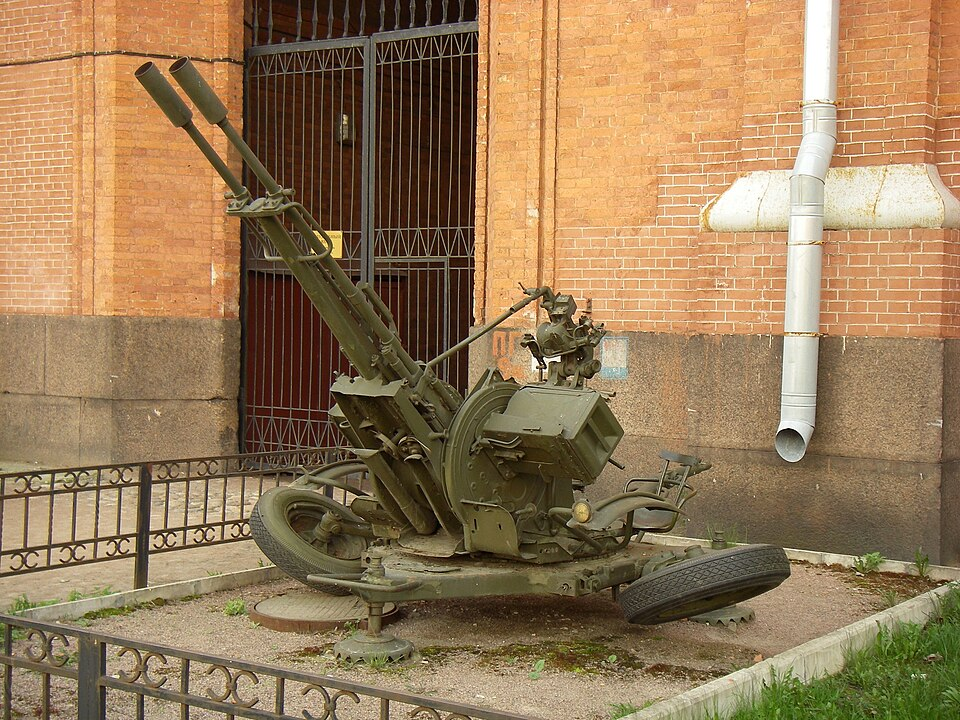
\includegraphics{../images/przeciwlotnicze/zu-23-2_1.jpg}
\caption{ZU-23-2 --- widok z boku}
\end{figure}

\begin{center}\rule{0.5\linewidth}{0.5pt}\end{center}

\subsection{Opis}\label{opis-37}

ZU-23-2 (Zenitnaja Ustanovka) to radzieckie sprzężone działko
przeciwlotnicze kalibru 23 mm, wprowadzone do służby w 1960 roku. Jest
jednym z najbardziej rozpowszechnionych systemów przeciwlotniczych na
świecie --- znalazło się na wyposażeniu ponad 60 armii. Pomimo niskiej
masy (950 kg) wyróżnia się niszczycielską szybkostrzelnością: 2000
strz./min teoretycznie, 400 strz./min praktycznie na jedną lufę. Poza
obroną plot. powszechnie montowane na ciężarówkach i BTR-ach jako broń
wsparcia piechoty. Używane przez obie strony w Ukrainie.

\subsection{Dane techniczne}\label{dane-techniczne-37}

\begin{longtable}[]{@{}
  >{\raggedright\arraybackslash}p{(\columnwidth - 2\tabcolsep) * \real{0.5263}}
  >{\raggedright\arraybackslash}p{(\columnwidth - 2\tabcolsep) * \real{0.4737}}@{}}
\toprule\noalign{}
\begin{minipage}[b]{\linewidth}\raggedright
Parametr
\end{minipage} & \begin{minipage}[b]{\linewidth}\raggedright
Wartość
\end{minipage} \\
\midrule\noalign{}
\endhead
\bottomrule\noalign{}
\endlastfoot
Typ & Holowane sprzężone działko przeciwlotnicze \\
Kraj produkcji & ZSRR \\
Rok wprowadzenia & 1960 \\
Masa & 950 kg \\
Kaliber & 23 mm (nabój 23×152B) \\
Liczba luf & 2 \\
Szybkostrzelność & 2000 strz./min (cykliczna); 400 strz./min (praktyczna
/ lufę) \\
Prędkość wylotowa & 970--980 m/s (BZT/OFZ); 1220 m/s (APDS-T) \\
Skuteczny zasięg poziomy & 2000--2500 m \\
Skuteczny pułap & 1500--2000 m \\
Kąt podniesienia lufy & −10° do +90° \\
Obsługa & 2 osoby (celowniczy + dowódca); pełen etat: 6 żołnierzy \\
\end{longtable}

\subsection{Charakterystyczne cechy
rozpoznawcze}\label{charakterystyczne-cechy-rozpoznawcze-37}

\begin{quote}
Jak odróżnić ZU-23-2 od innych działek plot.:
\end{quote}

\begin{itemize}
\tightlist
\item
  \textbf{Dwie lufy 23 mm na dwukołowej przyczepie} --- wyjątkowo lekka
  i kompaktowa; całość na małej przyczepce, w pozycji bojowej koła
  odchylają się na boki i działo opiera się na płytach oporowych
\item
  \textbf{Skrzynki amunicyjne prostopadle do osi luf} --- dwie
  50-nabojowe skrzynki po obu stronach działka zamontowane pod kątem
  prostym do luf (wyraźna wizualna cecha)
\item
  \textbf{Tłumiki płomienia na końcach obu luf} --- charakterystyczne
  ``kielichy'' / szczeliny na końcach luf
\item
  \textbf{Bardzo mała masa} --- wyraźnie lżejsze i mniejsze niż S-60
  (4660 kg) czy ZSU-23-4 (19 t)
\item
  \textbf{Często montowane na MT-LB lub ciężarówkach} --- jako
  ``technical'' z działkiem na dachu
\end{itemize}

\subsection{Ciekawostka}\label{ciekawostka-37}

\begin{quote}
W Finlandii ZU-23-2 ma ksywę ``Sergei''. Lufy przegrzewają się po ok.
100 strzałach --- dlatego zestaw ma zawsze dwie pary luf zapasowych. W
2020 roku etiopscy żołnierze w Somalii zestrzelili z ZU-23 cywilny
samolot transportujący moskitiery, myląc go z samolotem-bomba. W
Ukrainie działka te są powszechnie montowane na MT-LB, BTR-80 i
pick-upach jako broń wsparcia walki.
\end{quote}

\section{ZSU-23-4 Szyłka --- samobieżne działko
przeciwlotnicze}\label{zsu-23-4-szyux142ka-samobieux17cne-dziaux142ko-przeciwlotnicze}

\subsubsection{ZSU-23-4 Shilka Self-Propelled AA Gun \textbar{} ЗСУ-23-4
«Шилка»}\label{zsu-23-4-shilka-self-propelled-aa-gun-ux437ux441ux443-23-4-ux448ux438ux43bux43aux430}

\begin{figure}
\centering
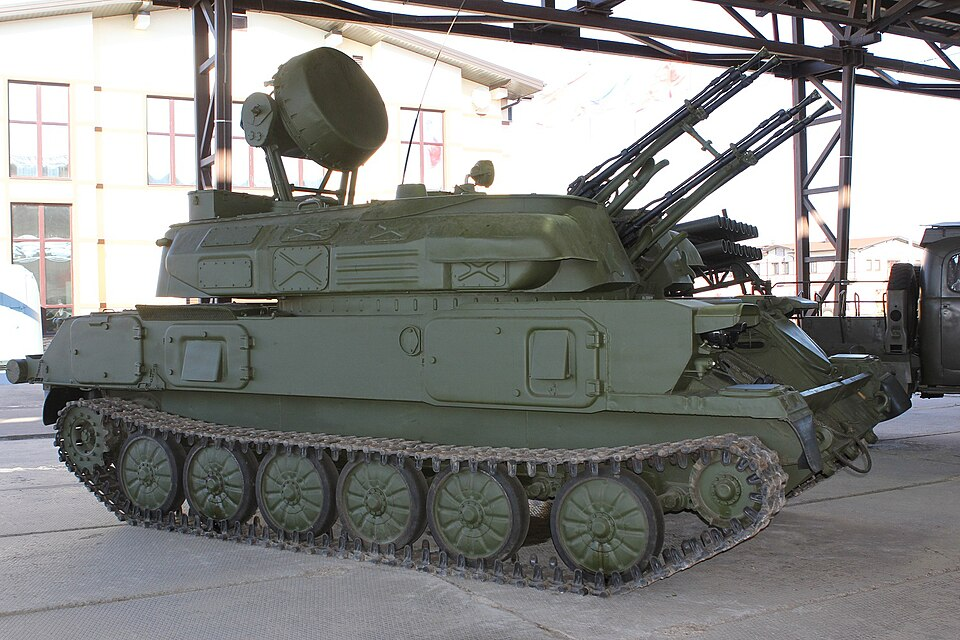
\includegraphics{../images/przeciwlotnicze/zsu-23-4_1.jpg}
\caption{ZSU-23-4 Szyłka --- widok z boku}
\end{figure}

\begin{center}\rule{0.5\linewidth}{0.5pt}\end{center}

\subsection{Opis}\label{opis-38}

ZSU-23-4 Szyłka to radziecka samobieżna zenitnaja samochódnaja ustanovka
z poczwórnie sprzężonymi armatami 23 mm, wprowadzona do służby w 1965
roku. Łączna szybkostrzelność 4 luf wynosi 3400--4000 strz./min --- co
pozwala na kompletne wyczerpanie 2000 nabojów w 30 sekund. Posiada
własny radar RPK-2 ``Toboł'' (NATO: Gun Dish) do autonomicznego
śledzenia celów. Była standardem p-lot. pułków i dywizji Układu
Warszawskiego. Dziś modyfikowana w Ukrainie do zwalczania dronów i
użycia w walkach miejskich.

\subsection{Dane techniczne}\label{dane-techniczne-38}

\begin{longtable}[]{@{}ll@{}}
\toprule\noalign{}
Parametr & Wartość \\
\midrule\noalign{}
\endhead
\bottomrule\noalign{}
\endlastfoot
Typ & Samobieżne działko przeciwlotnicze \\
Kraj produkcji & ZSRR \\
Rok wprowadzenia & 1965 \\
Masa & 19 t \\
Długość & 6,54 m \\
Szerokość & 3,13 m \\
Wysokość (z radarem) & 3,57 m \\
Uzbrojenie & 4× armata automatyczna 23 mm 2A7 (system AZP-23
``Amur'') \\
Zapas amunicji & 2000 nabojów (4×500) \\
Szybkostrzelność & 3400--4000 strz./min (łącznie) \\
Skuteczny zasięg / pułap & 2,5 km / 1,5 km \\
Radar & RPK-2 ``Toboł'' (NATO: Gun Dish), zasięg wykrywania 20 km \\
Silnik & V-6R diesel, 280 KM \\
Prędkość maks. & 50 km/h \\
Zasięg & 450 km \\
Załoga & 4 osoby (kierowca, dowódca, działonowy, operator radaru) \\
\end{longtable}

\subsection{Charakterystyczne cechy
rozpoznawcze}\label{charakterystyczne-cechy-rozpoznawcze-38}

\begin{quote}
Jak odróżnić ZSU-23-4 od innych pojazdów p-lot.:
\end{quote}

\begin{itemize}
\tightlist
\item
  \textbf{Radar ``talerz'' z tyłu wieży} --- okrągła antena radaru na
  składanych wspornikach, wyraźnie widoczna nad dachem wieży;
  podniesiony wygląda jak mała antena satelitarna
\item
  \textbf{Blok czterech długich luf 23 mm z przodu wieży} --- cztery
  lufy złączone w jedną masywną grupę, wycelowane w górę w pozycji
  marszowej
\item
  \textbf{Duża, obudowana spawana wieża pośrodku podwozia} --- zakrywa
  niemal cały kadłub; brak pancerza reaktywnego, cienkie ściany
\item
  \textbf{6 kół nośnych z gumowymi bandażami} --- podwozie PT-76/GM-575,
  koła jednolite z dużymi okrągłymi otworami
\item
  \textbf{Brak wieżyczki dowódcy} --- gładki dach wieży bez kopuły;
  wejście przez duże włazy na górze
\end{itemize}

\subsection{Ciekawostka}\label{ciekawostka-38}

\begin{quote}
Afgańczycy nazywali Szyłkę ``maszyną do szycia'' od charakterystycznego
dźwięku 4 szybkostrzelnych luf. Wewnętrzny przelicznik balistyczny 1A7
SRP waży 180 kg i składa się z 60 silniczków i 110 osi zębatych ---
czysto mechaniczny komputer z lat 60. W Ukrainie Szyłki są
przebudowywane na systemy ``Doniec'' (wieża na podwoziu T-80UD) i
``Rokacz'' (nowoczesny radar + rakiety Igła).
\end{quote}

\section{S-60 --- holowane działko przeciwlotnicze 57
mm}\label{s-60-holowane-dziaux142ko-przeciwlotnicze-57-mm}

\subsubsection{S-60 (AZP S-60) Anti-Aircraft Gun \textbar{} АЗП
С-60}\label{s-60-azp-s-60-anti-aircraft-gun-ux430ux437ux43f-ux441-60}

\begin{figure}
\centering
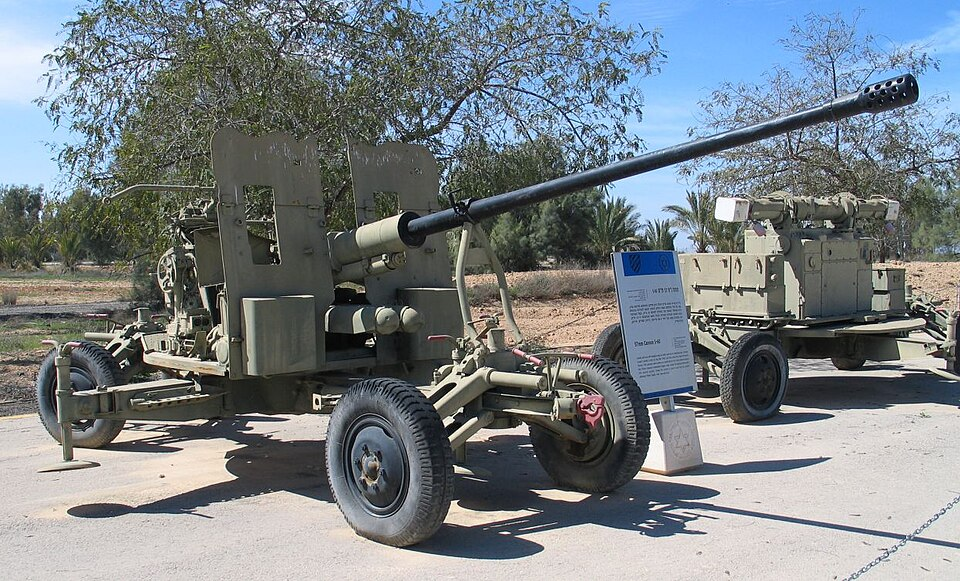
\includegraphics{../images/przeciwlotnicze/s-60_1.jpg}
\caption{S-60 --- holowane działko przeciwlotnicze 57 mm}
\end{figure}

\begin{center}\rule{0.5\linewidth}{0.5pt}\end{center}

\subsection{Opis}\label{opis-39}

S-60 (57 mm AZP S-60) to radziecka jednolufowa armata przeciwlotnicza
kalibru 57 mm, wprowadzona do służby w 1950 roku. Zaprojektowana na
bazie zdobycznych niemieckich prototypów z II wojny światowej, przez
dekady stanowiła trzon pułkowej artylerii przeciwlotniczej Układu
Warszawskiego i była eksportowana do ponad 40 krajów. Działa z systemem
kierowania ogniem SON-9 i przelicznikiem PUAZO-6-60, dzięki czemu może
zwalczać cele na pułapie do 6000 m. W Ukrainie obie strony używają S-60
zarówno jako klasycznej broni p-lot., jak i artylerii polowej.

\subsection{Dane techniczne}\label{dane-techniczne-39}

\begin{longtable}[]{@{}
  >{\raggedright\arraybackslash}p{(\columnwidth - 2\tabcolsep) * \real{0.5263}}
  >{\raggedright\arraybackslash}p{(\columnwidth - 2\tabcolsep) * \real{0.4737}}@{}}
\toprule\noalign{}
\begin{minipage}[b]{\linewidth}\raggedright
Parametr
\end{minipage} & \begin{minipage}[b]{\linewidth}\raggedright
Wartość
\end{minipage} \\
\midrule\noalign{}
\endhead
\bottomrule\noalign{}
\endlastfoot
Typ & Holowana armata przeciwlotnicza \\
Kraj produkcji & ZSRR \\
Rok wprowadzenia & 1950 \\
Masa & 4660 kg \\
Kaliber & 57 mm (nabój 57×347mmSR) \\
Szybkostrzelność & 105--120 strz./min (cykliczna); 70 strz./min
(praktyczna) \\
Prędkość wylotowa & 1000 m/s \\
Skuteczny zasięg poziomy & 6000 m (radar) / 4000 m (optyka) \\
Kąt podniesienia & −4° do +85° \\
System KO & SON-9 / PUAZO-6-60 (radar Grom-2 10 cm) \\
Obsługa & 7 osób \\
\end{longtable}

\subsection{Charakterystyczne cechy
rozpoznawcze}\label{charakterystyczne-cechy-rozpoznawcze-39}

\begin{quote}
Jak odróżnić S-60 od ZU-23-2 i innych działek p-lot.:
\end{quote}

\begin{itemize}
\tightlist
\item
  \textbf{Jedna gruba lufa 57 mm} --- w odróżnieniu od dwulufowego
  ZU-23-2; lufa wyraźnie grubsza i dłuższa
\item
  \textbf{Duże cztery koła + cztery wysięgniki stabilizujące} ---
  holowana na 4 kołach, w pozycji bojowej 4 ramiona rozkładają się na
  boki i unoszą koła od ziemi
\item
  \textbf{Masywna tarcza ochronna dla obsługi} --- charakterystyczna
  prostokątna osłona po lewej stronie lufy
\item
  \textbf{Wyraźnie cięższa od ZU-23-2} --- 4660 kg vs 950 kg; widać to
  po rozmiarach łoża i kół
\item
  \textbf{Brak sprzęgnięcia} --- pojedyncza lufa, nie podwójna jak w
  ZU-23-2 lub poczwórna jak w ZSU-23-4
\end{itemize}

\subsection{Ciekawostka}\label{ciekawostka-39}

\begin{quote}
Radzieccy konstruktorzy oparli S-60 na zdobytych niemieckich prototypach
z WWII --- w tym na działku 5,5 cm Gerät 58. Przelicznik PUAZO-5A
powstał z kolei na bazie niemieckiego kalkulatora ``Lambda''. W Ukrainie
Rosjanie montują S-60 na dachach MT-LB, a separatyści LNR wsadzili go w
miejsce wieży T-55, tworząc improwizowany ``czołg przeciwdronowy''.
Ukraina używa S-60 jako artylerii polowej --- działo trafia cel na 6,1
km.
\end{quote}

\section{2K22 Tunguska --- samobieżny zestaw
rakietowo-artyleryjski}\label{k22-tunguska-samobieux17cny-zestaw-rakietowo-artyleryjski}

\subsubsection{2K22 Tunguska SPAAG \textbar{} 2К22
«Тунгуска»}\label{k22-tunguska-spaag-2ux43a22-ux442ux443ux43dux433ux443ux441ux43aux430}

\begin{figure}
\centering
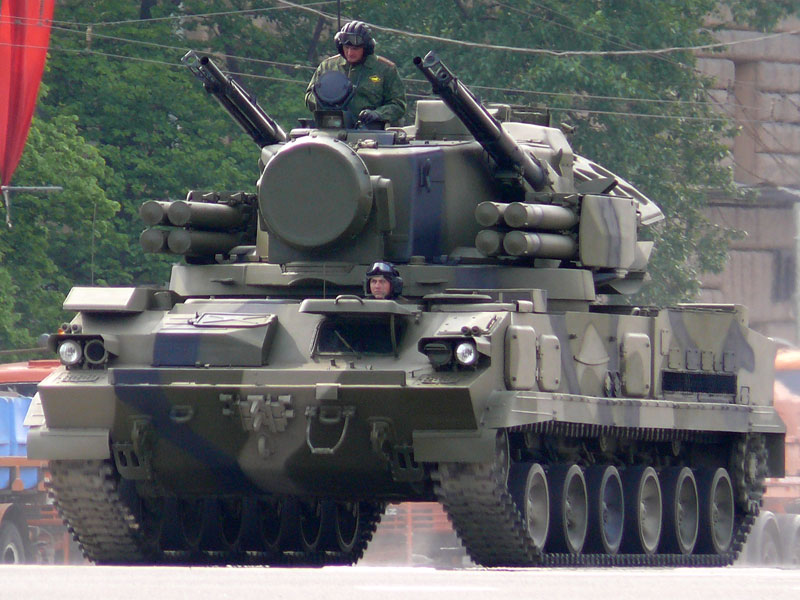
\includegraphics{../images/przeciwlotnicze/2k22-tunguska_1.jpg}
\caption{2K22 Tunguska --- widok z boku}
\end{figure}

\begin{center}\rule{0.5\linewidth}{0.5pt}\end{center}

\subsection{Opis}\label{opis-40}

2K22 Tunguska to rosyjski samobieżny zestaw przeciwlotniczy (SPAAG)
łączący dwie chłodzone cieczą armaty automatyczne 30 mm z 8 wyrzutniami
rakiet 9M311. Wprowadzony do służby 8 września 1982 roku, przeznaczony
do ochrony wojsk lądowych przed śmigłowcami, samolotami szturmowymi i
dronami na dystansie 0--8 km. Reaktywny czas otwarcia ognia z armat
wynosi zaledwie 8--10 sekund. Posiada własny radar Hot Shot do
wykrywania (18 km) i śledzenia celów. Używany przez obie strony w
Ukrainie.

\subsection{Dane techniczne}\label{dane-techniczne-40}

\begin{longtable}[]{@{}
  >{\raggedright\arraybackslash}p{(\columnwidth - 2\tabcolsep) * \real{0.5263}}
  >{\raggedright\arraybackslash}p{(\columnwidth - 2\tabcolsep) * \real{0.4737}}@{}}
\toprule\noalign{}
\begin{minipage}[b]{\linewidth}\raggedright
Parametr
\end{minipage} & \begin{minipage}[b]{\linewidth}\raggedright
Wartość
\end{minipage} \\
\midrule\noalign{}
\endhead
\bottomrule\noalign{}
\endlastfoot
Typ & Samobieżny zestaw rakietowo-artyleryjski \\
Kraj produkcji & ZSRR / Rosja \\
Rok wprowadzenia & 1982 (dostawy od 1984) \\
Masa & ok. 35 000 kg \\
Długość & 7,90 m \\
Szerokość & 3,25 m \\
Uzbrojenie artyleryjskie & 2× armata 30 mm 2A38M (dwulufowe),
szybkostrzelność łączna 3900--5000 strz./min \\
Zasięg armat & 0,2--4,0 km \\
Uzbrojenie rakietowe & 8× rakieta 9M311 (lub 9M311-M1 w Tunguska-M1) \\
Zasięg rakiet & 8 km (9M311) / 10 km (9M311-M1) \\
Maksymalny pułap & 3500 m \\
Radar & 1RL144 ``Hot Shot'' --- wykrywanie 18 km, śledzenie 16 km \\
Silnik & V-46 diesel, 710 KM \\
Prędkość maks. & 65 km/h \\
Załoga & 4 osoby \\
\end{longtable}

\subsection{Charakterystyczne cechy
rozpoznawcze}\label{charakterystyczne-cechy-rozpoznawcze-40}

\begin{quote}
Jak odróżnić 2K22 Tunguska od Pancyra i innych zestawów plot.:
\end{quote}

\begin{itemize}
\tightlist
\item
  \textbf{Podwozie gąsienicowe} --- Tunguska zawsze na gąsienicach (6
  kół nośnych); Pancyr-S1 zwykle na kołowym podwoziu 8×8
\item
  \textbf{Dwa bloki po 4 wyrzutnie rurowe po bokach wieży} ---
  prostokątne kontenery z rakietami, wyraźnie odstawione od kadłuba po
  obu stronach wieży
\item
  \textbf{Dwie bardzo długie lufy 30 mm pod blokami rakiet} --- po
  jednej parabolicznej grupie luf pod każdym blokiem wyrzutni
\item
  \textbf{Paraboliczny radar z tyłu wieży + okrągły radar śledzący z
  przodu} --- dwa wyraźnie różne kształty anten na jednej wieży
\item
  \textbf{Masywna, obrotowa wieża pośrodku kadłuba} --- wieża zajmuje
  niemal całą górną część pojazdu
\end{itemize}

\subsection{Ciekawostka}\label{ciekawostka-40}

\begin{quote}
Rozwój Tunguski niemal porzucono na rzecz 9K33 Osa, ale analiza wykazała
słabość Osy wobec śmigłowców wyłaniających się zza osłon --- Osa
potrzebuje 30 sekund na reakcję, Tunguska 8--10 sekund. Ukraina posiada
ok. 75 sztuk; w Ukrainie Tunguski operują bezpośrednio na linii frontu,
ukryte pod kamuflażem z gałęzi.
\end{quote}

\section{9K33 Osa --- samobieżny zestaw
rakietowy}\label{k33-osa-samobieux17cny-zestaw-rakietowy}

\subsubsection{9K33 Osa (SA-8 Gecko) SAM System \textbar{} 9К33
«Оса»}\label{k33-osa-sa-8-gecko-sam-system-9ux43a33-ux43eux441ux430}

\begin{figure}
\centering
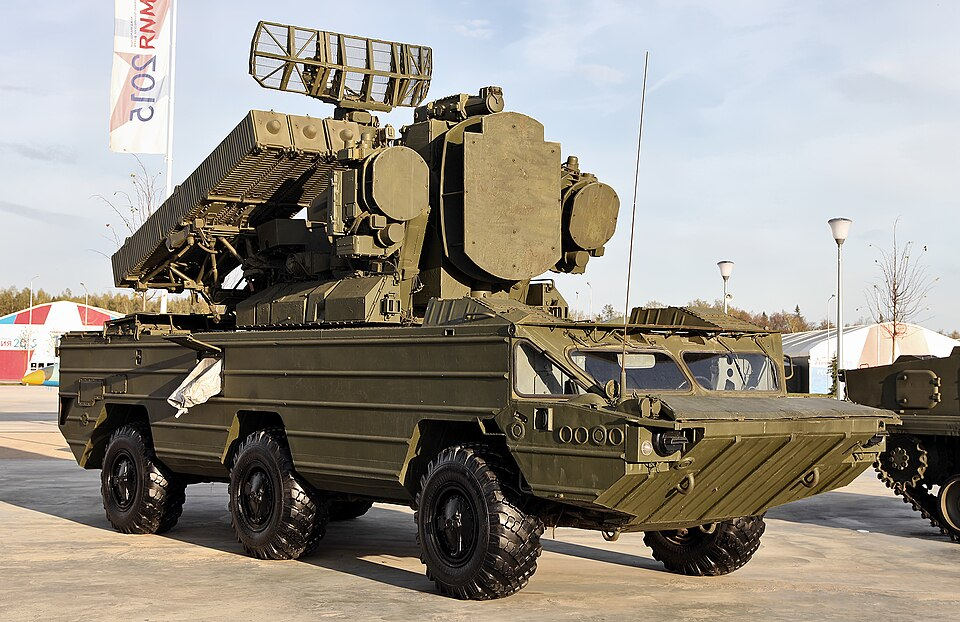
\includegraphics{../images/przeciwlotnicze/9k33-osa_1.jpg}
\caption{9K33 Osa --- widok z boku}
\end{figure}

\begin{center}\rule{0.5\linewidth}{0.5pt}\end{center}

\subsection{Opis}\label{opis-41}

9K33 Osa (NATO: SA-8 Gecko) to radziecki samobieżny zestaw
przeciwlotniczy krótkiego zasięgu, wprowadzony do służby w 1971--1972
roku. Był pierwszym na świecie systemem p-lot., który w pełni
zintegrował radar wykrywania, radar śledzenia i wyrzutnie rakiet na
jednym pojeździe (typ TELAR). W wersji Osa-AKM niesie 6 rakiet 9M33M3 o
zasięgu do 15 km. Pojazd jest w pełni amfibijny (prędkość w wodzie 8
km/h), napędzany silnikiem diesla D20K300. Zarówno Ukraina jak i Rosja
używają go w wojnie, a Ukraina zmodernizowała swoje egzemplarze do
odpalania rakiet R-73 (``FrankenSAM'').

\subsection{Dane techniczne}\label{dane-techniczne-41}

\begin{longtable}[]{@{}ll@{}}
\toprule\noalign{}
Parametr & Wartość \\
\midrule\noalign{}
\endhead
\bottomrule\noalign{}
\endlastfoot
Typ & Samobieżny zestaw rakietowy krótkiego zasięgu \\
Kraj produkcji & ZSRR \\
Rok wprowadzenia & 1971--1972 \\
Masa & 17,5 t \\
Długość & 9,14 m \\
Szerokość & 2,75 m \\
Podwozie & Kołowe BAZ-5937, 6×6 \\
Rakieta & 9M33 / 9M33M3 \\
Zasięg rakiet & 2--9 km (9M33) / do 15 km (9M33M3) \\
Pułap & 50--5000 m (9M33) / do 12 000 m (9M33M3) \\
Prędkość rakiety & ok. 1020 m/s (≈Mach 3) \\
Liczba rakiet & 6 (wersja Osa-AKM) \\
Radar & 1S51M3 (NATO: Land Roll) --- wykrywanie 30 km, śledzenie 20
km \\
Silnik & D20K300 diesel \\
Prędkość maks. (droga) & 80 km/h \\
Prędkość w wodzie & 8 km/h \\
Zasięg & 500 km \\
Załoga & 5 osób \\
\end{longtable}

\subsection{Charakterystyczne cechy
rozpoznawcze}\label{charakterystyczne-cechy-rozpoznawcze-41}

\begin{quote}
Jak odróżnić 9K33 Osę od innych zestawów p-lot.:
\end{quote}

\begin{itemize}
\tightlist
\item
  \textbf{Kołowe podwozie 6×6} --- jedyny kompletny TELAR p-lot. na 6
  kołach; żadne inne opancerzone TELAR-y na kołach 6×6 nie wyglądają
  podobnie
\item
  \textbf{Eliptyczna antena wykrywająca na szczycie} --- obracająca się
  elipsa widoczna na samym wierzchołku bloku radarowego
\item
  \textbf{Dwa ``talerze'' namierzające po bokach bloku radarowego} ---
  dwie paraboliczne anteny (jak ``oczy'') flankujące centralną okrągłą
  antenę śledzącą
\item
  \textbf{6 żebrowanych kontenerów startowych po obu bokach bloku
  radarowego} --- prostokątne, wyraźnie żebrowane pojemniki na rakiety
  (3+3)
\item
  \textbf{Brak uzbrojenia artyleryjskiego} --- w odróżnieniu od Tunguski
  i Pancyra, Osa nie ma dział
\end{itemize}

\subsection{Ciekawostka}\label{ciekawostka-41}

\begin{quote}
W 1987 roku wojska południowoafrykańskie zdobyły pod Cuito Cuanavale
nienaruszoną Osę --- pierwszą w rękach państwa spoza Układu
Warszawskiego. Ukraina stworzyła zestaw ``FrankenSAM'' montując na
wyrzutniach Osy rakiety lotnicze R-73 po wyczerpaniu oryginalnych 9M33.
Radar Osy może jednocześnie naprowadzać dwie rakiety na jeden cel na
różnych częstotliwościach.
\end{quote}

\section{System rakietowy dalekiego zasięgu
S-300}\label{system-rakietowy-dalekiego-zasiux119gu-s-300}

\subsubsection{S-300 Long-Range Air Defence System \textbar{}
С-300}\label{s-300-long-range-air-defence-system-ux441-300}

\begin{figure}
\centering
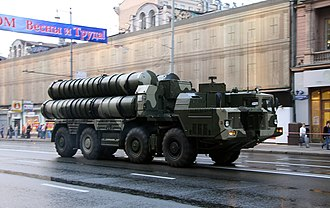
\includegraphics{../images/przeciwlotnicze/s-300_1.jpg}
\caption{S-300 na paradzie zwycięstwa w Moskwie 2009}
\end{figure}

\begin{center}\rule{0.5\linewidth}{0.5pt}\end{center}

\subsection{Opis}\label{opis-42}

S-300 (NATO: SA-10 Grumble) to rodzina radzieckich i rosyjskich systemów
rakiet przeciwlotniczych dalekiego zasięgu, wprowadzona do służby w 1978
roku. Jest jednym z najskuteczniejszych systemów obrony przeciwlotniczej
na świecie --- przez dekady stanowił kręgosłup radzieckiej i rosyjskiej
obrony powietrznej. System może jednocześnie śledzić i atakować wiele
celów powietrznych, w tym samoloty, śmigłowce, pociski manewrujące, a
nowsze warianty także pociski balistyczne. S-300 jest rozmieszczany na
samochodach ciężarowych (wersja mobilna) lub stacjonarnie. Doświadczenia
z Ukrainy pokazały zarówno jego skuteczność, jak i podatność na ataki
dronów i precyzyjnych rakiet manewrujących.

\subsection{Dane techniczne}\label{dane-techniczne-42}

\begin{longtable}[]{@{}ll@{}}
\toprule\noalign{}
Parametr & Wartość \\
\midrule\noalign{}
\endhead
\bottomrule\noalign{}
\endlastfoot
Typ & Samobieżny system rakiet p-lot dalekiego zasięgu \\
Kraj produkcji & ZSRR / Rosja \\
Rok wprowadzenia & 1978 (S-300P); liczne modernizacje \\
Zasięg (maks.) & 40--400 km (zależnie od wariantu i pocisku) \\
Pułap raziący & 25 m -- 27 000 m \\
Pociski & 5V55 / 48N6 / 40N6 (zależnie od wersji) \\
Naprowadzanie & Półaktywny radar / Aktywny radar (nowsze wersje) \\
Pojazd bazowy & Ciężarówka MAZ-543 (8×8) lub gąsienicowy \\
Wyrzutnia & 4 pociski na TEL \\
Czas gotowości & 5 minut (bojowa) \\
\end{longtable}

\subsection{Charakterystyczne cechy
rozpoznawcze}\label{charakterystyczne-cechy-rozpoznawcze-42}

\begin{quote}
Jak rozpoznać system S-300 w terenie lub na zdjęciach:
\end{quote}

\begin{itemize}
\tightlist
\item
  \textbf{Pionowe wyrzutnie na ciężarówce 8×8 (TEL):} charakterystyczne
  cztery pionowe pojemniki startowe na platformie ciężarówki MAZ-543 ---
  pociski wystrzeliwane są pionowo w górę, a następnie skręcają w
  kierunku celu (VLS)
\item
  \textbf{Duża kabina radarowa na osobnym pojeździe:} radar śledzenia
  celów (36D6 lub 64N6) to charakterystyczna duża obracająca się antena
  --- zawsze na osobnym pojeździe towarzyszącym baterii
\item
  \textbf{Cylindryczne pojemniki transportowo-startowe:} każdy pocisk
  jest zamknięty w długim walcowatym pojemniku (ok. 7 m długości) --- 4
  takie pojemniki widoczne pionowo na platformie TEL
\item
  \textbf{Biało-szare kontenery z charakterystycznym zielonym
  oznakowaniem:} bateria S-300 składa się z kilku pojazdów o podobnym
  kształcie pudełkowych kontenerów na ciężarówkach
\item
  \textbf{Długie anteny i kable łączące pojazdy:} na stanowisku ogniowym
  bateria S-300 jest widoczna jako skupisko kilku pojazdów połączonych
  kablami
\item
  \textbf{Charakterystyczny ``dźwięk'' pasywnego radaru:} w dzień ---
  obracająca się duża antena na pojeździe radiolokacyjnym to nieodłączny
  element każdej baterii
\end{itemize}

\subsection{Ciekawostka}\label{ciekawostka-42}

\begin{quote}
Zakup systemu S-300 przez Turcję (NATO) w 2019 roku wywołał największy
kryzys dyplomatyczny w historii Sojuszu --- USA wykluczyły Turcję z
programu myśliwców F-35 i nałożyły sankcje. Paradoksalnie Turcja nigdy
nie włączyła S-300 do swojej obrony powietrznej i system stał nieaktywny
w magazynach --- zakup był prawdopodobnie kartą przetargową w
negocjacjach z USA, a nie prawdziwą potrzebą militarną.
\end{quote}

\section{System rakietowy dalekiego zasięgu S-400
Triumf}\label{system-rakietowy-dalekiego-zasiux119gu-s-400-triumf}

\subsubsection{S-400 Triumf Air Defence System \textbar{} С-400
«Триумф»}\label{s-400-triumf-air-defence-system-ux441-400-ux442ux440ux438ux443ux43cux444}

\begin{figure}
\centering
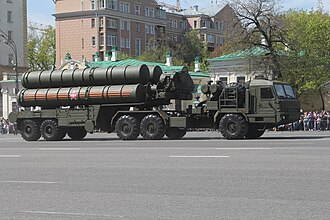
\includegraphics{../images/przeciwlotnicze/s-400_1.jpg}
\caption{S-400 Triumf --- zdjęcie systemu}
\end{figure}

\begin{center}\rule{0.5\linewidth}{0.5pt}\end{center}

\subsection{Opis}\label{opis-43}

S-400 Triumf (NATO: SA-21 Growler) to rosyjski system rakiet
przeciwlotniczych dalekiego zasięgu, zatwierdzony do służby w 2007 roku
jako bezpośredni następca S-300. Jest uważany za jeden z
najskuteczniejszych systemów obrony powietrznej na świecie i stanowi
jeden z najważniejszych rosyjskich produktów eksportowych w dziedzinie
uzbrojenia. System może zwalczać samoloty, śmigłowce, drony, pociski
manewrujące oraz pociski balistyczne na odległość do 400 km i pułapie do
30 km. Zdolność do jednoczesnego śledzenia 300 celów i angażowania 36 z
nich czyni go niezwykle trudnym do przełamania dla przeciwnika. Zakup
S-400 przez Turcję (2019) i Indie wywołał poważne napięcia dyplomatyczne
z USA.

\subsection{Dane techniczne}\label{dane-techniczne-43}

\begin{longtable}[]{@{}ll@{}}
\toprule\noalign{}
Parametr & Wartość \\
\midrule\noalign{}
\endhead
\bottomrule\noalign{}
\endlastfoot
Typ & System rakiet p-lot dalekiego zasięgu \\
Kraj produkcji & Rosja \\
Rok wprowadzenia & 2007 \\
Zasięg maks. (pocisk 40N6E) & 400 km \\
Zasięg maks. (pocisk 48N6DM) & 240 km \\
Zasięg krótki (pocisk 9M96M) & 120 km \\
Pułap raziący & do 30 000 m \\
Naprowadzanie & Aktywny / półaktywny radar (zależnie od pocisku) \\
Pojazd bazowy & MZKT-7930 (8×8) \\
Śledzenie celów & do 300 jednocześnie \\
Równoczesne zaangażowanie & do 36 celów \\
\end{longtable}

\subsection{Charakterystyczne cechy
rozpoznawcze}\label{charakterystyczne-cechy-rozpoznawcze-43}

\begin{quote}
Jak odróżnić S-400 od S-300:
\end{quote}

\begin{itemize}
\tightlist
\item
  \textbf{Nowszy, bardziej smukły kształt pojemników startowych:}
  pojemniki TEL S-400 są nieco dłuższe i smuklejsze niż S-300; montowane
  na nowszych ciężarówkach MZKT-7930 o wyraźnie innym kształcie kabiny
\item
  \textbf{Kabina ciężarówki MZKT-7930 --- charakterystyczny prostokątny
  kształt:} pojazd bazowy S-400 (MZKT) ma bardziej nowoczesną, bardziej
  prostokątną kabinę niż starsze MAZ-543 S-300
\item
  \textbf{8 pojemników startowych na TEL (lub 4):} w zależności od
  wariantu pojazd TEL może nieść 4 duże lub 8 mniejszych pojemników;
  konfiguracja 8×9M96 jest charakterystyczna tylko dla S-400
\item
  \textbf{Radar 91N6E ``Big Bird'' --- duża eliptyczna antena na
  wysięgniku:} radar S-400 ma charakterystyczną dużą, eliptyczną antenę
  na składanym maszcie --- wyraźnie inną od radarów S-300
\item
  \textbf{Zestaw pojazdów --- zawsze minimum 4--5 jednostek:} bateria
  S-400 to zawsze zgrupowanie kilku pojazdów: radar, wyrzutnie, pojazd
  dowodzenia, zasilacz
\item
  \textbf{Pionowy start i moment skręcenia pocisku:} S-400 startuje
  pionowo (jak S-300) --- po odpaleniu widoczny jest biały dym z pionowo
  lecącego pocisku, który po sekundzie gwałtownie skręca w kierunku celu
\end{itemize}

\subsection{Ciekawostka}\label{ciekawostka-43}

\begin{quote}
S-400 jest pierwszym na świecie systemem, który może używać czterech
różnych typów pocisków jednocześnie --- od krótkiego zasięgu 9M96E (40
km) po pociski dalekiego zasięgu 40N6E (400 km). Pozwala to jednej
baterii na zwalczanie zarówno dronów latających nisko, jak i samolotów
AWACS krążących wysoko z dala od frontu. Producent (Ałmaz-Antiej)
twierdzi, że S-400 może zestrzelić nawet cele stealth --- choć ta
właściwość nie była dotąd potwierdzona w warunkach bojowych.
\end{quote}

\section{System rakietowy krótkiego zasięgu
Tor}\label{system-rakietowy-kruxf3tkiego-zasiux119gu-tor}

\subsubsection{Tor Air Defence System \textbar{} Тор
(9К330)}\label{tor-air-defence-system-ux442ux43eux440-9ux43a330}

\begin{figure}
\centering
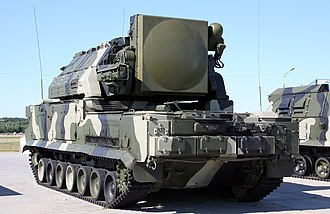
\includegraphics{../images/przeciwlotnicze/tor_1.jpg}
\caption{Tor-M1 --- system na poligonie}
\end{figure}

\begin{center}\rule{0.5\linewidth}{0.5pt}\end{center}

\subsection{Opis}\label{opis-44}

Tor (NATO: SA-15 Gauntlet) to radziecki/rosyjski samobieżny system
obrony przeciwlotniczej krótkiego zasięgu, wprowadzony do służby w 1986
roku. Przeznaczony jest do ochrony wojsk na polu walki przed samolotami,
śmigłowcami, pociskami manewrującymi i dronami na małych i średnich
wysokościach. Tor jest systemem w pełni zintegrowanym --- jeden pojazd
gąsienicowy zawiera zarówno radar, wyrzutnię 8 pocisków, jak i system
kierowania ogniem. Może zwalczać cele na odległość do 12 km i pułapie do
6000 m. System zyskał smutną sławę w 2020 roku, gdy irański Tor-M1
zestrzelił ukraiński samolot pasażerski Lot 752 --- zdarzenie, które
Iran początkowo zaprzeczał przez kilka dni.

\subsection{Dane techniczne}\label{dane-techniczne-44}

\begin{longtable}[]{@{}ll@{}}
\toprule\noalign{}
Parametr & Wartość \\
\midrule\noalign{}
\endhead
\bottomrule\noalign{}
\endlastfoot
Typ & Samobieżny system rakietowy p-lot krótkiego zasięgu \\
Kraj produkcji & ZSRR / Rosja \\
Rok wprowadzenia & 1986 (Tor-M1: 1991, Tor-M2: 2016) \\
Zasięg maks. & 12 km (Tor-M1), 16 km (Tor-M2) \\
Pułap raziący & do 6 000 m (Tor-M2: do 10 000 m) \\
Liczba rakiet & 8 gotowych do odpalenia \\
Czas reakcji & 5--8 sekund \\
Pojazd bazowy & Gąsienicowy GM-569 \\
Prędkość pojazdu & 65 km/h \\
Masa bojowa & 34 t \\
Załoga & 3 osoby \\
\end{longtable}

\subsection{Charakterystyczne cechy
rozpoznawcze}\label{charakterystyczne-cechy-rozpoznawcze-44}

\begin{quote}
Jak rozpoznać Tor w terenie:
\end{quote}

\begin{itemize}
\tightlist
\item
  \textbf{Duża prostokątna skrzynia z 8 pionowymi wyrzutniami na
  wierzchu:} górna część pojazdu to charakterystyczna prostokątna
  platforma z 8 wyrzutniami pionowymi --- widoczna z każdej strony jako
  ``blok'' na wierzchu kadłuba
\item
  \textbf{Dwa radary --- jeden z przodu, jeden z tyłu:} na wieżyczce
  Tora zawsze widać dwie różne anteny: jedną do wykrywania celów
  (większa, obracająca się szybko) i jedną do naprowadzania (mniejsza,
  nieruchoma lub wolnoobrotowa)
\item
  \textbf{Gąsienicowe podwozie bez wieży bocznej:} Tor porusza się na
  gąsienicach i wygląda jak ``jeżdżący kontener'' --- brak tradycyjnej
  artyleryjskiej wieży z lufą jest natychmiastowym rozpoznaniem
\item
  \textbf{Charakterystyczna kwadratowa antena z przodu pojazdu:} panel
  antenowy radaru śledzenia celów na przedniej górnej ścianie pojazdu
  --- prostokątny, z charakterystycznym wzorem otworów
\item
  \textbf{Dużo wyższy niż szerszy --- sylwetka ``wieży'':} Tor jest
  pojazdem nieproporcjonalnie wysokim w stosunku do długości --- jego
  sylwetka bardziej przypomina wieżę niż pojazd bojowy
\item
  \textbf{Brak lufy --- tylko pionowe pojemniki:} nie ma żadnej
  widocznej lufy czy armaty --- tylko pionowe rury wyrzutni na wierzchu,
  co go natychmiast odróżnia od systemów artyleryjskich
\end{itemize}

\subsection{Ciekawostka}\label{ciekawostka-44}

\begin{quote}
W lipcu 2014 roku ukraińskie wojsko podało, że samolot transportowy
An-26 lecący na wysokości 6500 m został zestrzelony pociskiem, który
``nie mógł'' dosięgnąć takiej wysokości według oficjalnych parametrów
Tora. Analitycy wywnioskwali, że Rosja użyła wariantu Tor-M2U z
nieopublikowanymi parametrami zasięgu. Ta historia pokazuje, że
oficjalne dane techniczne systemów rosyjskich są często celowo zaniżane.
\end{quote}

\section{Artyleryjsko-rakietowy system p-lot
Pancerz-S1}\label{artyleryjsko-rakietowy-system-p-lot-pancerz-s1}

\subsubsection{Pantsir-S1 Air Defence System \textbar{}
Панцирь-С1}\label{pantsir-s1-air-defence-system-ux43fux430ux43dux446ux438ux440ux44c-ux4411}

\begin{figure}
\centering
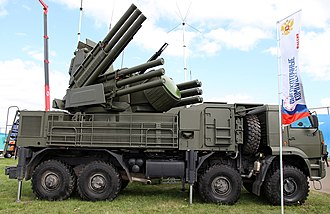
\includegraphics{../images/przeciwlotnicze/pantsir_1.jpg}
\caption{Pancerz-S1 na targach lotniczych MAKS 2013}
\end{figure}

\begin{center}\rule{0.5\linewidth}{0.5pt}\end{center}

\subsection{Opis}\label{opis-45}

Pancerz-S1 (ros. Панцирь-С1 --- pancerz) to rosyjski samobieżny
artyleryjsko-rakietowy system obrony przeciwlotniczej bliskiego zasięgu,
wchodzący do służby od 2012 roku. Łączy w jednym pojeździe dwa typy
uzbrojenia: rakiety ziemia-powietrze (zasięg do 20 km) oraz podwójne
działka automatyczne 30 mm (zasięg do 4 km), co zapewnia obronę
wielowarstwową. System przeznaczony jest do ochrony obiektów
stacjonarnych i baterii S-300/S-400 przed samolotami, śmigłowcami,
dronami i pociskami manewrującymi. W wojnie w Ukrainie Pancerz-S1
poniósł znaczne straty od ukraińskich dronów --- co ujawniło jego
słabość wobec tanich, licznych BSL.

\subsection{Dane techniczne}\label{dane-techniczne-45}

\begin{longtable}[]{@{}ll@{}}
\toprule\noalign{}
Parametr & Wartość \\
\midrule\noalign{}
\endhead
\bottomrule\noalign{}
\endlastfoot
Typ & Samobieżny system artyleryjsko-rakietowy p-lot \\
Kraj produkcji & Rosja \\
Rok wprowadzenia & 2012 \\
Zasięg rakiet & do 20 km \\
Zasięg działek 30 mm & do 4 km \\
Pułap raziący (rakiety) & do 15 000 m \\
Pułap raziący (działka) & do 3 000 m \\
Pojazd bazowy & KAMAZ-6560 (8×8) lub gąsienicowy GM-352 \\
Obsługa & 3 osoby + kierowca \\
Rakiety na wozie & 12 pocisków 57E6 \\
\end{longtable}

\subsection{Charakterystyczne cechy
rozpoznawcze}\label{charakterystyczne-cechy-rozpoznawcze-45}

\begin{quote}
Jak rozpoznać Pancerz-S1:
\end{quote}

\begin{itemize}
\tightlist
\item
  \textbf{Dwa duże radary na dachu --- jeden śledzący, jeden
  naprowadzający:} charakterystyczna para anten radarowych na wieżyczce
  --- duża antena śledzenia i mniejsza naprowadzania --- jednocześnie
  obracające się w różnym rytmie
\item
  \textbf{Dwa bloki po 6 rakiet po bokach wieżyczki:} po obu stronach
  centralnej wieży widoczne są dwa charakterystyczne prostokątne bloki z
  6 pionowymi pojemnikami rakietowymi każdy --- łącznie 12 rakiet
\item
  \textbf{Dwie lufy 30 mm wystające z boków wieżyczki:}
  charakterystyczne podwójne lufy działek automatycznych umieszczone
  symetrycznie po lewej i prawej stronie wieżyczki, poniżej bloków
  rakietowych
\item
  \textbf{Pojazd bazowy KAMAZ z charakterystyczną kabiną:} ciężarówka
  KAMAZ-6560 ma charakterystyczną prostokątną kabinę --- inne proporcje
  niż pojazdy S-300/S-400
\item
  \textbf{Okrągła wieżyczka z ``ramionami'' rakietowymi:} z góry widać
  centralną okrągłą wieżyczkę z dwoma ``ramionami'' po bokach --- każde
  ramię to blok rakietowy
\item
  \textbf{Krótszy i szerszy niż S-300/S-400:} Pancerz jest wyraźnie
  niższy i mniej smukły od wyrzutni S-300 --- cały system mieści się na
  jednym pojeździe, podczas gdy S-300 potrzebuje kilku
\end{itemize}

\subsection{Ciekawostka}\label{ciekawostka-45}

\begin{quote}
W Syrii nagranie drona kamikaze niszczy Pancerz-S1, który w tym czasie
stał nieruchomo bez aktywnego radaru --- system był ``uśpiony''.
Analitycy NATO stwierdzili, że to właśnie jest główna słabość Pancerza:
radar musi być aktywny, żeby system działał, a aktywny radar zdradza
pozycję. Twórcy systemu odpowiedzieli, że Pancerz nigdy nie miał działać
samodzielnie --- zawsze w zestawie z S-300/S-400, pod ich ``parasolem''.
\end{quote}

\section{Przenośny system rakietowy 9K34 Strieła-3
(MANPADS)}\label{przenoux15bny-system-rakietowy-9k34-strieux142a-3-manpads}

\subsubsection{9K34 Strela-3 Man-Portable Air Defence System \textbar{}
9К34
«Стрела-3»}\label{k34-strela-3-man-portable-air-defence-system-9ux43a34-ux441ux442ux440ux435ux43bux430-3}

\begin{center}\rule{0.5\linewidth}{0.5pt}\end{center}

\begin{figure}
\centering
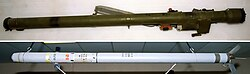
\includegraphics{../images/przeciwlotnicze/strela-3_1.jpg}
\caption{9K34 Striełła-3 --- MANPADS}
\end{figure}

\subsection{Opis}\label{opis-46}

9K34 Strieła-3 (NATO: SA-14 Gremlin) to radziecki przenośny system
rakietowy przeciwlotniczego wprowadzony do służby w 1974 roku jako
ulepszenie starszej Strieły-2. Kluczowym postępem w stosunku do
poprzednika jest zastosowanie modulowanego szukacza IR chłodzonego
azotem, co znacznie zwiększyło odporność na zakłócenia i flary termiczne
oraz umożliwiło atakowanie celów na kursie zbliżającym (nie tylko od
tyłu). Strieła-3 była masowo eksportowana do sojuszniczych armii i
ruchów wyzwoleńczych --- dziś jest w rękach aktorów państwowych i
niepaństwowych w kilkudziesięciu krajach. W armii rosyjskiej zastąpiła
ją Igła, ale Strieła-3 jest wciąż spotykana w magazynach i na polach
bitew Ukrainy i Bliskiego Wschodu.

\subsection{Dane techniczne}\label{dane-techniczne-46}

\begin{longtable}[]{@{}ll@{}}
\toprule\noalign{}
Parametr & Wartość \\
\midrule\noalign{}
\endhead
\bottomrule\noalign{}
\endlastfoot
Typ & Przenośny system rakietowy p-lot (MANPADS) \\
Kraj produkcji & ZSRR \\
Rok wprowadzenia & 1974 \\
Zasięg maks. & 4 500 m \\
Pułap raziący & 3 000 m (cele wolne), 1 800 m (odrzutowce) \\
Prędkość pocisku & 470 m/s \\
Masa gotowa do strzału & 16 kg \\
Głowica bojowa & 1,17 kg (odłamkowo-kumulacyjna) \\
Naprowadzanie & Pasywny IR, FM-modulowany, chłodzony azotem \\
\end{longtable}

\subsection{Charakterystyczne cechy
rozpoznawcze}\label{charakterystyczne-cechy-rozpoznawcze-46}

\begin{quote}
Jak odróżnić Striełę-3 od Igły i Stingera:
\end{quote}

\begin{itemize}
\tightlist
\item
  \textbf{Piaskowo-brązowy lub oliwkowy kolor tuby:} Strieła-3 jest
  zazwyczaj w kolorze piaskowo-brązowym lub oliwkowym --- Igła jest
  ciemnozielona; kolor to szybki (choć nie zawsze pewny) odróżnik
\item
  \textbf{Starsza, prostsza głowica poszukująca z przodu:} głowica IR
  Strieły-3 jest nieco szersza i mniej smukła niż w Igle; widoczna po
  zdjęciu zaślepki jako okrągłe szkło szukacza
\item
  \textbf{Brak podwójnego zakresu spektralnego:} Strieła-3 ma szukacz
  jednopasmowy (podczerwień) --- nie ma dodatkowego filtra UV jak Igła;
  to różnica techniczna niewidoczna z zewnątrz, ale wpływająca na
  podatność na flary
\item
  \textbf{Krótszy blok zasilania niż Igła:} akumulator/zasilacz z tyłu
  wyrzutni Strieły-3 jest nieco krótszy i lżejszy niż masywniejszy blok
  Igły-S
\item
  \textbf{Brak identyfikatora IFF:} starsza Strieła-3 standardowo nie ma
  wyposażenia do rozpoznania swój-obcy; nowsze wersje Igły mają IFF jako
  opcję
\item
  \textbf{Tuba wyrzutni nieco cieńsza od Igły:} proporcje wyrzutni
  Strieły-3 są nieco smuklejsze; przy bezpośrednim porównaniu różnica
  jest zauważalna
\end{itemize}

\subsection{Ciekawostka}\label{ciekawostka-46}

\begin{quote}
Strieła-3 (SA-14) stała się pierwszym MANPADS-em który zestrzelił
izraelski śmigłowiec bojowy w 1982 roku podczas inwazji na Liban. PLO
użyła jej do zestrzelenia UH-1 Huey --- co było wielkim zaskoczeniem dla
Izraelczyków, którzy nie spodziewali się tak zaawansowanej broni w
rękach nieregularnych. To zdarzenie zmieniło reguły gry dla wszystkich
sił lotniczych operujących na niskich pułapach nad obszarami konfliktu.
\end{quote}

\section{Przenośny system rakietowy 9K38 Igła
(MANPADS)}\label{przenoux15bny-system-rakietowy-9k38-igux142a-manpads}

\subsubsection{9K38 Igla Man-Portable Air Defence System \textbar{} 9К38
«Игла»}\label{k38-igla-man-portable-air-defence-system-9ux43a38-ux438ux433ux43bux430}

\begin{figure}
\centering
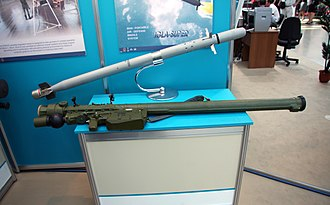
\includegraphics{../images/przeciwlotnicze/igla_1.jpg}
\caption{Igła-S na wystawie IDELF-2008}
\end{figure}

\begin{center}\rule{0.5\linewidth}{0.5pt}\end{center}

\subsection{Opis}\label{opis-47}

9K38 Igła (ros. «Игла» --- igła; NATO: SA-18 Grouse) to radziecka
przenośna wyrzutnia rakiet przeciwlotniczych (MANPADS), wprowadzona do
służby w 1983 roku. Jest następcą systemu 9K34 Strieła-3 i znacznie
skuteczniejsza od poprzednika --- pocisk ma podwójny tryb naprowadzania
i jest odporniejszy na flary termiczne. Igła może być obsługiwana przez
jednego żołnierza i jest zdolna do zestrzelenia samolotów odrzutowych,
śmigłowców i dronów latających na małych wysokościach. System był masowo
dostarczany przez ZSRR i Rosję do sojuszniczych armii i ruchów
partyzanckich --- co sprawiło, że dziś jest w rękach dziesiątek
państwowych i niepaństwowych podmiotów na całym świecie.

\subsection{Dane techniczne}\label{dane-techniczne-47}

\begin{longtable}[]{@{}ll@{}}
\toprule\noalign{}
Parametr & Wartość \\
\midrule\noalign{}
\endhead
\bottomrule\noalign{}
\endlastfoot
Typ & Przenośny system rakietowy p-lot (MANPADS) \\
Kraj produkcji & ZSRR / Rosja \\
Rok wprowadzenia & 1983 (Igła-1: 1981, Igła-S: 2004) \\
Zasięg maks. & 5--6 km (Igła-S: do 6 km) \\
Pułap raziący & do 3 500 m \\
Prędkość pocisku & Mach 1,9 \\
Masa gotowa do strzału & 17,9--19 kg \\
Głowica bojowa & 1,17 kg (Igła) / 2,5 kg (Igła-S) \\
Naprowadzanie & Pasywny IR (podczerwień), podwójny zakres spektralny \\
\end{longtable}

\subsection{Charakterystyczne cechy
rozpoznawcze}\label{charakterystyczne-cechy-rozpoznawcze-47}

\begin{quote}
Jak rozpoznać Igłę w terenie:
\end{quote}

\begin{itemize}
\tightlist
\item
  \textbf{Długa zielona lub oliwkowa rura na ramieniu strzelca:}
  charakterystyczna cylindryczna wyrzutnia (\textasciitilde1,7 m
  długości) trzymana na ramieniu --- żadna inna broń nie wygląda tak
  samo z odległości
\item
  \textbf{Charakterystyczny czarny „cel'' na końcu lufy:} z przodu
  wyrzutni widoczna jest zaślepka z charakterystycznym wzorem optycznym
  (znacznik IR) --- po zdjęciu zaślepki widać głowicę poszukującą
\item
  \textbf{Niebiesko-zielony kolor odróżnia od starej Strieły:} Igła jest
  zazwyczaj w kolorze ciemnooliwkowym lub zielonym, podczas gdy starsza
  Strieła-2 jest w kolorze piaskowo-brązowym (choć kolor zależy od
  operatora)
\item
  \textbf{Duży blok elektroniczny z boku tuby --- zasilanie i IFF:} z
  boku lub z tyłu wyrzutni widoczny jest charakterystyczny blok
  elektroniczny z akumulatorem chłodzącym --- musi być aktywowany przed
  strzałem
\item
  \textbf{Strzelec w pozycji stojącej z rurą na ramieniu:} sposób
  trzymania Igły (rura na prawym ramieniu, głowa po lewej stronie) jest
  charakterystyczny i odróżnia go od RPG czy granatnika
\item
  \textbf{Brak celownika optycznego --- tylko kimograf termiczny:} Igła
  nie ma lunetki --- strzelec obserwuje cel przez prosty kimograf
  (wizjer) i słyszy sygnał dźwiękowy gdy głowica ``złapie'' cel
\end{itemize}

\subsection{Ciekawostka}\label{ciekawostka-47}

\begin{quote}
Igła odegrała kluczową rolę w wojnie w Afganistanie --- ale po stronie
mudżahedinów. USA dostarczyły im system FIM-92 Stinger, a ZSRR próbował
bronić swoich śmigłowców. Paradoksalnie, po zakończeniu zimnej wojny CIA
przez lata próbowała odkupić od różnych podmiotów nielegalne Igły i
Stingery --- bo obawiała się, że terroryści użyją ich do zestrzelenia
samolotów pasażerskich. Szacuje się, że do dziś na czarnym rynku krąży
kilka tysięcy niekontrolowanych egzemplarzy Igły.
\end{quote}

\section{Przenośny system rakietowy 9K333 Wierba
(MANPADS)}\label{przenoux15bny-system-rakietowy-9k333-wierba-manpads}

\subsubsection{9K333 Verba Man-Portable Air Defence System \textbar{}
9К333
«Верба»}\label{k333-verba-man-portable-air-defence-system-9ux43a333-ux432ux435ux440ux431ux430}

\begin{figure}
\centering
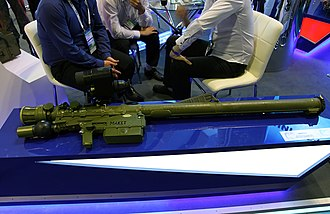
\includegraphics{../images/przeciwlotnicze/verba_1.jpg}
\caption{9K333 Verba --- na targach MAKS 2015}
\end{figure}

\begin{center}\rule{0.5\linewidth}{0.5pt}\end{center}

\subsection{Opis}\label{opis-48}

9K333 Wierba (ros. «Верба» --- wierzba; NATO: SA-25) to rosyjski
przenośny system rakietowy czwartej generacji, przyjęty do służby w 2014
roku jako następca Igły-S. Kluczową innowacją jest wielospektralny
szukacz IR pracujący jednocześnie w trzech zakresach: ultrafiolet,
bliski IR i średni IR --- co czyni Wierbę praktycznie odporną na
nowoczesne flary termiczne i aktywne zakłócacze. System może zwalczać
samoloty, śmigłowce, drony i pociski manewrujące o małej sygnaturze
cieplnej. Wierba jest podłączona do systemu zautomatyzowanego
zarządzania ogniem --- strzelec może otrzymać dane o celu elektronicznie
bez konieczności samodzielnego wyszukiwania. Jest to aktualnie
najnowocześniejszy MANPADS w arsenale rosyjskim.

\subsection{Dane techniczne}\label{dane-techniczne-48}

\begin{longtable}[]{@{}
  >{\raggedright\arraybackslash}p{(\columnwidth - 2\tabcolsep) * \real{0.5263}}
  >{\raggedright\arraybackslash}p{(\columnwidth - 2\tabcolsep) * \real{0.4737}}@{}}
\toprule\noalign{}
\begin{minipage}[b]{\linewidth}\raggedright
Parametr
\end{minipage} & \begin{minipage}[b]{\linewidth}\raggedright
Wartość
\end{minipage} \\
\midrule\noalign{}
\endhead
\bottomrule\noalign{}
\endlastfoot
Typ & Przenośny system rakietowy p-lot 4. generacji (MANPADS) \\
Kraj produkcji & Rosja \\
Rok wprowadzenia & 2014 (oficjalnie 2015) \\
Zasięg maks. & 6 500 m \\
Pułap raziący & do 4 500 m \\
Prędkość pocisku & Mach 1,5 (500 m/s) \\
Masa gotowa do strzału & 17,25 kg \\
Głowica bojowa & 1,5 kg \\
Naprowadzanie & Pasywny IR multispektralny (UV + bliski IR + średni
IR) \\
\end{longtable}

\subsection{Charakterystyczne cechy
rozpoznawcze}\label{charakterystyczne-cechy-rozpoznawcze-48}

\begin{quote}
Jak odróżnić Wierbę od Igły i starszych MANPADS:
\end{quote}

\begin{itemize}
\tightlist
\item
  \textbf{Nowocześniejsza, bardziej smukła tuba z wyraźnie inną
  głowicą:} głowica szukająca Wierby jest cieńsza i dłuższa niż Igły ---
  wynika to z trójzakresowego szukacza wymagającego więcej optyki
\item
  \textbf{Elektroniczny celownik z wyświetlaczem (opcja):} zestaw Wierby
  może być sprzężony z naziemnym stanowiskiem docelowania z ekranem ---
  widocznym jako dodatkowy element przy stanowisku strzeleckim
\item
  \textbf{Ciemnozielony kolor tuby (jak Igła):} Wierba jest w
  standardowym rosyjskim kolorze zielonym --- jak Igła; odróżnienie od
  Igły na podstawie samego koloru jest trudne bez bliższego przyjrzenia
  się
\item
  \textbf{Dłuższa i smuklejsza tuba niż Igła:} Wierba jest nieznacznie
  dłuższa od Igły --- widoczne przy bezpośrednim porównaniu lub
  zestawieniu zdjęć
\item
  \textbf{Nowszy blok elektroniczny z większą powierzchnią:} blok
  zasilania/chłodzenia z tyłu jest nieco większy niż w starszej Igle, z
  nowocześniejszą obudową
\item
  \textbf{Stanowisko zintegrowane z systemem zarządzania polem walki:}
  Wierba jest zazwyczaj częścią sieciowego zestawu z anteniną danych ---
  strzelec ma dodatkowy moduł komunikacji przy sobie
\end{itemize}

\subsection{Ciekawostka}\label{ciekawostka-48}

\begin{quote}
Wierba była jednym z pierwszych rosyjskich systemów uzbrojenia
przetestowanych w walce niemal natychmiast po wprowadzeniu do służby ---
trafiła do Syrii w 2015 roku, rok po przyjęciu do uzbrojenia. Analitycy
oceniali, że Rosja celowo przyspieszyła wdrożenie bojowe, by zebrać dane
z rzeczywistych warunków walki i sprawdzić skuteczność trójspektralnego
szukacza przeciw amunicji USA. To ``battlefield testing'' nowej broni
stało się od tamtej pory rosyjską doktryną operacyjną.
\end{quote}

\section{Przeciwpancerny pocisk kierowany 9K111
Fagot}\label{przeciwpancerny-pocisk-kierowany-9k111-fagot}

\subsubsection{9K111 Fagot Anti-Tank Guided Missile \textbar{} 9К111
«Фагот»}\label{k111-fagot-anti-tank-guided-missile-9ux43a111-ux444ux430ux433ux43eux442}

\begin{figure}
\centering
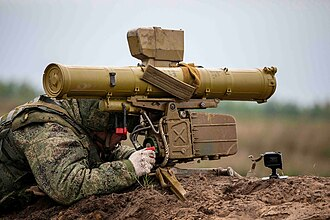
\includegraphics{../images/przeciwpancerne/fagot_1.jpg}
\caption{9K111 Fagot --- zestaw z wyrzutnią}
\end{figure}

\begin{center}\rule{0.5\linewidth}{0.5pt}\end{center}

\subsection{Opis}\label{opis-49}

9K111 Fagot (NATO: AT-4 Spigot) to radziecka przenośna wyrzutnia
przeciwpancernych pocisków kierowanych, wprowadzona do służby w 1970
roku. System przeznaczony jest do rażenia pojazdów opancerzonych,
fortyfikacji i pozycji ogniowych na odległość do 2500 m. Pocisk
naprowadzany jest metodą SACLOS (półautomatyczne naprowadzanie po linii
wzroku) za pomocą przewodu --- obsługujący śledzi cel przez celownik, a
elektronika automatycznie koryguje lot pocisku. Fagot jest lekki,
przenośny i może być użyty przez 2-osobową obsługę. Pomimo
zaawansowanego wieku jest wciąż stosowany przez armię rosyjską i
dziesiątki innych armii na całym świecie.

\subsection{Dane techniczne}\label{dane-techniczne-49}

\begin{longtable}[]{@{}ll@{}}
\toprule\noalign{}
Parametr & Wartość \\
\midrule\noalign{}
\endhead
\bottomrule\noalign{}
\endlastfoot
Typ & Przenośny ppk (przewodowy SACLOS) \\
Kraj produkcji & ZSRR / Rosja \\
Rok wprowadzenia & 1970 \\
Zasięg min. / maks. & 70 / 2 500 m \\
Warhead & Kumulacyjna HEAT \\
Przenikanie pancerza & 400--600 mm stali jednolitej (RHA) \\
Prędkość pocisku & 186 m/s (maks.) \\
Czas lotu do 2500 m & \textasciitilde13 s \\
Masa zestawu & \textasciitilde22 kg (wyrzutnia + pocisk) \\
Obsługa & 2 osoby \\
\end{longtable}

\subsection{Charakterystyczne cechy
rozpoznawcze}\label{charakterystyczne-cechy-rozpoznawcze-49}

\begin{quote}
Jak rozpoznać zestaw Fagot w terenie:
\end{quote}

\begin{itemize}
\tightlist
\item
  \textbf{Prostokątna wyrzutnia na trójnogu z celownikiem optycznym:}
  wyrzutnia ma charakterystyczny prostokątny kształt z boku ---
  przypomina teleskop lub kamerę na trójnogu; żaden inny system ppk nie
  wygląda tak samo
\item
  \textbf{Pudełkowy pojemnik startowy z pociskom:} pocisk w pojemniku
  startowym (metalowa skrzynka \textasciitilde120 cm długości) jest
  wyraźnie widoczny po bokach lub z tyłu wyrzutni przed odpaleniem
\item
  \textbf{Przewód sterowania wysuwający się po starcie:}
  charakterystyczny cienki drut (przewód sygnałowy) rozwijający się za
  lecącym pociskiem --- widoczny na nagraniach jako błyszcząca linia za
  pociskiem
\item
  \textbf{Biały dym odrzutowy przy starcie:} odpalenie daje
  charakterystyczny biały/szary dym po bokach wyrzutni (silnik
  startowy), a następnie pocisk leci z czerwonawym śladem spalin
\item
  \textbf{Mały rozmiar zestawu:} całość jest kompaktowa i może być
  transportowana przez dwie osoby --- wyrzutnia nie zajmuje więcej
  miejsca niż lekki karabin maszynowy na trójnogu
\item
  \textbf{Celownik optyczny 9Sz16 po lewej stronie wyrzutni:}
  charakterystyczny duży celownik optyczny wystający po lewej stronie
  cylindrycznej wieży wyrzutni
\end{itemize}

\subsection{Ciekawostka}\label{ciekawostka-49}

\begin{quote}
Fagot był pierwszym radzieckim ppk z systemem SACLOS --- obsługa musi
jedynie utrzymać krzyżyk celownika na celu, a elektronika sama koryguje
pocisk. To ogromny postęp w stosunku do poprzednich systemów pierwszej
generacji (9M14 Malyutka), gdzie operator musiał ręcznie sterować
pociskiem joystickiem. Statystyki z Afganistanu i Bliskiego Wschodu
pokazują, że prawdopodobieństwo trafienia wzrosło z 50--60\% (systemy 1.
generacji) do ponad 90\% przy SACLOS.
\end{quote}

\section{Przeciwpancerny pocisk kierowany 9M113
Konkurs}\label{przeciwpancerny-pocisk-kierowany-9m113-konkurs}

\subsubsection{9M113 Konkurs Anti-Tank Guided Missile \textbar{} 9М113
«Конкурс»}\label{m113-konkurs-anti-tank-guided-missile-9ux43c113-ux43aux43eux43dux43aux443ux440ux441}

\begin{center}\rule{0.5\linewidth}{0.5pt}\end{center}

\subsection{Opis}\label{opis-50}

9M113 Konkurs (NATO: AT-5 Spandrel) to radziecki przewodowy ppk systemu
SACLOS, wprowadzony do służby w 1974 roku jako ulepszenie wcześniejszego
Fagota. Znacznie zwiększony zasięg (do 4000 m) i lepsza głowica
kumulacyjna (600--800 mm przebicia) sprawiły, że Konkurs stał się
podstawowym ciężkim ppk na wyposażeniu BWP, transporterów i zestawów
naziemnych. Może być stosowany zarówno z pojazdu (m.in. BMP-1, BTR-80A),
jak i z przenośnej wyrzutni naziemnej. Konkurs był jednym z najszerzej
stosowanych ppk na świecie --- Indie zamówiły ponad 15 000 pocisków,
używają go też Iran, Syria, Hezbollah i wiele innych podmiotów.

\subsection{Dane techniczne}\label{dane-techniczne-50}

\begin{longtable}[]{@{}ll@{}}
\toprule\noalign{}
Parametr & Wartość \\
\midrule\noalign{}
\endhead
\bottomrule\noalign{}
\endlastfoot
Typ & Ppk przewodowy SACLOS \\
Kraj produkcji & ZSRR / Rosja \\
Rok wprowadzenia & 1974 \\
Zasięg min. / maks. & 70 / 4 000 m \\
Warhead & Tandemowa HEAT (wersja 9M113M) \\
Przenikanie pancerza & 600 mm (oryginał), 750--800 mm (9M113M) \\
Prędkość pocisku & 208 m/s (maks.) \\
Masa zestawu naziemnego & \textasciitilde22 kg \\
Obsługa & 2--3 osoby \\
\end{longtable}

\subsection{Charakterystyczne cechy
rozpoznawcze}\label{charakterystyczne-cechy-rozpoznawcze-50}

\begin{quote}
Jak odróżnić Konkurs od Fagota:
\end{quote}

\begin{itemize}
\tightlist
\item
  \textbf{Wyrzutnia identyczna jak Fagot --- różnica w pocisku:}
  wyrzutnie Fagota i Konkursa są kompatybilne --- odróżnienie na
  pierwszy rzut oka jest trudne; Konkurs ma nieco dłuższy i grubszy
  pojemnik startowy pocisku
\item
  \textbf{Pojemnik startowy pocisku \textasciitilde130 cm vs
  \textasciitilde105 cm Fagota:} Konkurs ma wyraźnie dłuższy pojemnik
  transportowo-startowy --- przy bezpośrednim porównaniu różnica jest
  oczywista
\item
  \textbf{Montaż na BMP-1/2:} wyrzutnia Konkursa zamontowana na
  wieżyczce BWP ma charakterystyczny kształt z okrągłą głowicą
  poszukującą --- widoczna na szczycie wieżyczki BMP jako mała
  ``wysepka''
\item
  \textbf{Przewód sterowania (drut) rozwijający się za pociskiem:}
  identyczny jak w Fagocie --- cienki drut śledzący lot pocisku
\item
  \textbf{Biało-szary dym przy starcie, czerwona flara na rakiecie:}
  start pocisku jest bardzo podobny do Fagota --- krótki biały dym
  boczny, potem wyraźna czerwona flara na końcu pocisku w locie
\item
  \textbf{Trójnóg z wyrzutnią nieco wyższy niż Fagot:} zestaw naziemny
  Konkursa jest odrobinę wyższy i masywniejszy niż Fagot ze względu na
  cięższy pocisk
\end{itemize}

\subsection{Ciekawostka}\label{ciekawostka-50}

\begin{quote}
9M113 Konkurs był pierwszym radzieckim ppk, który trafił na czołny
izraelski czołg Merkava podczas wojny libańskiej w 1982 roku. Użyli go
członkowie PLO --- co spowodowało panikę w izraelskim sztabie, bo
uważano Merkavę za ``niezniszczalną''. Okazało się, że reaktywny pancerz
Blazer skutecznie neutralizuje pierwotną głowicę Konkursa, ale wersja
tandemowa (9M113M) pojawiła się kilkanaście lat później właśnie w
odpowiedzi na takie pancerze reaktywne.
\end{quote}

\section{Lekki ppk 9K115 Metis}\label{lekki-ppk-9k115-metis}

\subsubsection{9K115 Metis Anti-Tank Guided Missile \textbar{} 9К115
«Метис»}\label{k115-metis-anti-tank-guided-missile-9ux43a115-ux43cux435ux442ux438ux441}

\begin{center}\rule{0.5\linewidth}{0.5pt}\end{center}

\subsection{Opis}\label{opis-51}

9K115 Metis (NATO: AT-7 Saxhorn) to radziecki lekki przenośny ppk,
wprowadzony do służby w 1979 roku. Przeznaczony dla jednostek szczebla
kompania jako lekka broń przeciwpancerna obsługiwana przez 2-osobowy
zespół. Metis strzelający nabojem kumulacyjnym przebija do 460 mm
pancerza, co pozwala na zwalczanie starszych czołgów i wszystkich
pojazdów opancerzonych lżejszych. W odróżnieniu od Fagota/Konkursa,
Metis jest wyraźnie lżejszy i kompaktowszy, co czyni go bronią
piechotną, nie wymagającą pojazdu. Zastąpiony przez ulepszoną wersję
Metis-M z głowicą tandemową, ale oryginał wciąż spotykany w magazynach i
w użyciu bojowym.

\subsection{Dane techniczne}\label{dane-techniczne-51}

\begin{longtable}[]{@{}ll@{}}
\toprule\noalign{}
Parametr & Wartość \\
\midrule\noalign{}
\endhead
\bottomrule\noalign{}
\endlastfoot
Typ & Lekki ppk przewodowy SACLOS \\
Kraj produkcji & ZSRR \\
Rok wprowadzenia & 1979 \\
Zasięg min. / maks. & 40 / 1 000 m \\
Warhead & HEAT kumulacyjna \\
Przenikanie pancerza & 460 mm stali jednolitej (RHA) \\
Masa pocisku & 5,5 kg \\
Masa wyrzutni & 10,2 kg \\
Obsługa & 2 osoby \\
\end{longtable}

\subsection{Charakterystyczne cechy
rozpoznawcze}\label{charakterystyczne-cechy-rozpoznawcze-51}

\begin{quote}
Jak odróżnić Metis od Fagota i Metis-M:
\end{quote}

\begin{itemize}
\tightlist
\item
  \textbf{Znacznie mniejszy i lżejszy niż Fagot:} Metis jest wyraźnie
  kompaktowszy --- trójnóg jest niższy, wyrzutnia mniejsza, pojemnik
  pocisku krótszy (\textasciitilde90 cm vs \textasciitilde105 cm Fagota)
\item
  \textbf{Pojemnik pocisku bez wyraźnych żeber bocznych:} pojemnik
  Metisa jest gładszy i bardziej owalny niż Fagota, który ma żebra
  wzdłużne; przy bezpośrednim porównaniu widoczne
\item
  \textbf{Prosty, minimalistyczny trójnóg bez wbudowanego celownika:}
  wyrzutnia Metisa jest bardzo prosta --- małe rożki, mały celownik;
  bardziej spartańska konstrukcja niż Fagot
\item
  \textbf{Biały lub kremowy kolor pojemnika pocisku:} pojemniki Metisa
  są zazwyczaj białe lub kremowo-żółte z czarnymi oznaczeniami; Fagot
  często ma szary lub oliwkowy pojemnik
\item
  \textbf{Krótszy zasięg wymusza zbliżoną pracę z celem:} obserwując
  strzał Metisa --- operator musi być bliżej celu (max 1 km) niż z
  Fagotem (2,5 km) czy Konkursem (4 km)
\item
  \textbf{Mniejsza flara startowa przy odpaleniu:} Metis ma mniejszy
  silnik startowy --- start jest mniej efektowny, mniejszy wybuch dymu
  niż przy Konkursie
\end{itemize}

\subsection{Ciekawostka}\label{ciekawostka-51}

\begin{quote}
Metis ma jeden z najkrótszych zasięgów maksymalnych wśród ppk drugiej
generacji --- zaledwie 1000 m. To znaczy, że jego obsługa musiała
zbliżać się do czołgu na odległość, przy której celownicze w wieżyczce
mogli doskonale widzieć strzelców. W Afganistanie mudżahedinowie
(używający zdobycznych Metisów) odkryli, że strzał z Metisa jest niemal
operacją samobójczą na otwartym terenie. Dlatego system był używany
głównie z krótkich dystansów w terenie zurbanizowanym lub w zasadzkach w
wąskich dolinach.
\end{quote}

\section{Lekki ppk 9K115-2 Metis-M}\label{lekki-ppk-9k115-2-metis-m}

\subsubsection{9K115-2 Metis-M Anti-Tank Guided Missile \textbar{}
9К115-2
«Метис-М»}\label{k115-2-metis-m-anti-tank-guided-missile-9ux43a115-2-ux43cux435ux442ux438ux441-ux43c}

\begin{center}\rule{0.5\linewidth}{0.5pt}\end{center}

\subsection{Opis}\label{opis-52}

9K115-2 Metis-M (NATO: AT-13 Saxhorn-2) to rosyjski lekki przenośny ppk,
wprowadzony do służby w 1992 roku jako modernizacja systemu Metis.
Przeznaczony dla jednostek szczebla kompania --- obsługa 3-osobowa
przenosi cały system na plecach i może go rozwinąć do strzału w 15--20
sekund. Metis-M ma głowicę tandemową zdolną do przebicia ponad 800 mm
pancerza, co pozwala na niszczenie czołgów wyposażonych w pancerz
reaktywny ERA. Dostępna jest też głowica termobaryczna do niszczenia
umocnień i schronów. System jest kompaktowy, lekki i tani w porównaniu
do cięższych ppk, co czyni go popularnym na szczeblu kompania ---
zarówno w armii regularnej, jak i u niepaństwowych aktorów konfliktu.

\subsection{Dane techniczne}\label{dane-techniczne-52}

\begin{longtable}[]{@{}ll@{}}
\toprule\noalign{}
Parametr & Wartość \\
\midrule\noalign{}
\endhead
\bottomrule\noalign{}
\endlastfoot
Typ & Lekki ppk przewodowy SACLOS \\
Kraj produkcji & Rosja \\
Rok wprowadzenia & 1992 \\
Zasięg min. / maks. & 80 / 2 000 m (Metis-M1: do 2 000 m) \\
Warhead & Tandemowa HEAT / termobaryczna \\
Przenikanie pancerza & 800 mm (tandem), 900--980 mm (Metis-M1) \\
Masa pocisku & 13,8 kg \\
Masa wyrzutni & 10,2 kg \\
Szybkostrzelność & 3--4 strz./min \\
Obsługa & 3 osoby \\
\end{longtable}

\subsection{Charakterystyczne cechy
rozpoznawcze}\label{charakterystyczne-cechy-rozpoznawcze-52}

\begin{quote}
Jak odróżnić Metis-M od Fagota i Konkursa:
\end{quote}

\begin{itemize}
\tightlist
\item
  \textbf{Znacznie mniejsza i lżejsza wyrzutnia niż Fagot:} wyrzutnia
  Metisa-M jest wyraźnie mniejsza --- niższy trójnóg, mniejsza głowica
  celownicza --- można ją pomylić z prostym monocelem, nie z ppk
\item
  \textbf{Krótszy pojemnik pocisku niż Fagot:} pojemnik startowy Metisa
  jest krótszy i smuklejszy; łatwo odróżnić przy bezpośrednim porównaniu
\item
  \textbf{Wyrzutnia bez charakterystycznego ``teleskopu'' Fagota:}
  wizjer Fagota jest duży i charakterystyczny; Metis-M ma mniejszy,
  bardziej kompaktowy celownik
\item
  \textbf{Bardzo mały rozmiar całości --- system ``plecakowy'':} cały
  zestaw Metis-M mieści się w trzech plecakach noszonych przez trzech
  żołnierzy; żaden inny ppk nie jest tak kompaktowy w transporcie
\item
  \textbf{Białożółty kolor pojemnika startowego pocisku:} pojemniki
  pocisków Metisa mają charakterystyczny jasny (biały lub kremowy) kolor
  z żółtymi lub czarnymi oznaczeniami
\item
  \textbf{Mały prostokątny blok elektroniczny na wyrzutni:} z boku
  wyrzutni widoczny jest charakterystyczny mały czarny blok
  elektroniczny z kablem --- mniejszy niż w Fagocie i Konkursie
\end{itemize}

\subsection{Ciekawostka}\label{ciekawostka-52}

\begin{quote}
Metis-M jest jedynym rosyjskim ppk, który może być efektywnie
obsługiwany przez jeden oddział piechoty bez specjalistycznego pojazdu.
Trzyosobowy zespół może przenosić wyrzutnię i 5 pocisków na plecach,
rozwinąć system w niezamieszkałym terenie w mniej niż 30 sekund i zwinąć
go po strzale zanim przeciwnik zdąży odpowiedzieć. To właśnie ta
mobilność sprawia, że Metis-M jest ulubioną bronią oddziałów
dywersyjnych, sił specjalnych i nieregularnych.
\end{quote}

\section{Przeciwpancerny pocisk kierowany 9M133
Kornet}\label{przeciwpancerny-pocisk-kierowany-9m133-kornet}

\subsubsection{9M133 Kornet Anti-Tank Guided Missile \textbar{} 9М133
«Корнет»}\label{m133-kornet-anti-tank-guided-missile-9ux43c133-ux43aux43eux440ux43dux435ux442}

\begin{center}\rule{0.5\linewidth}{0.5pt}\end{center}

\subsection{Opis}\label{opis-53}

9M133 Kornet (NATO: AT-14 Spriggan) to rosyjski ppk trzeciej generacji z
naprowadzaniem laserowym, wprowadzony do służby w 1998 roku. Jest jednym
z najskuteczniejszych ppk na świecie --- głowica tandemowa przebija
ponad 1000 mm stali jednolitej po przebiciu przez pancerz reaktywny ERA,
co pozwala na niszczenie każdego współczesnego czołgu. Naprowadzanie
laserowe (beam-riding) zamiast przewodu sprawia, że Kornet jest
praktycznie odporny na zakłócenia elektromagnetyczne. Wariant Kornet-EM
ma zasięg do 10 km i potrafi atakować dwa cele jednocześnie. Stosowany z
różnych platform: przenośna wyrzutnia, pojazdy bojowe (BMP-3, Bumerang),
a nawet samobójcze łodzie i drony. Zestrzelił czołgi Merkava, Abrams i
Leopard 2.

\subsection{Dane techniczne}\label{dane-techniczne-53}

\begin{longtable}[]{@{}ll@{}}
\toprule\noalign{}
Parametr & Wartość \\
\midrule\noalign{}
\endhead
\bottomrule\noalign{}
\endlastfoot
Typ & Ppk laserowo naprowadzany (beam-riding) \\
Kraj produkcji & Rosja \\
Rok wprowadzenia & 1998 (Kornet-EM: 2012) \\
Zasięg min. / maks. & 100 / 5 500 m (Kornet-EM: do 10 000 m) \\
Warhead & Tandemowa HEAT / termobaryczna \\
Przenikanie pancerza & 1 000--1 200 mm za ERA (tandem) \\
Prędkość pocisku & 250 m/s (start) → 300 m/s \\
Naprowadzanie & Laserowe wiązką (SACLOS laserowy --- bez przewodu) \\
Obsługa & 2 osoby \\
\end{longtable}

\subsection{Charakterystyczne cechy
rozpoznawcze}\label{charakterystyczne-cechy-rozpoznawcze-53}

\begin{quote}
Jak odróżnić Kornet od Fagota, Konkursa i innych ppk:
\end{quote}

\begin{itemize}
\tightlist
\item
  \textbf{Brak przewodu sterowania --- pocisk leci bez druta:} to
  fundamentalna różnica od Fagota/Konkursa --- Kornet nie ma druta; za
  lecącym pociskiem nie ma ciągnącej się linii, tylko ślad spalin
\item
  \textbf{Wyrzutnia z dużym celownikiem laserowym:} wyrzutnia Korneta ma
  charakterystyczny duży teleskopowy celownik ze zintegrowanym laserem i
  kamerą termowizyjną (opcja) --- masywniejszy niż w Fagocie
\item
  \textbf{Pojemnik pocisku większy i cięższy niż Fagot:} pocisk Korneta
  jest grubszy i masywniejszy niż Fagota --- dłuższy kontener o innym
  kształcie przekroju
\item
  \textbf{Czarna / ciemnoszara tuba pojemnika startowego:} pojemnik
  pocisku Korneta jest zazwyczaj w kolorze ciemnoszarym lub czarnym z
  żółtymi oznaczeniami --- inne niż beżowo-szare Fagoty
\item
  \textbf{Wariant na pojeździe --- 2 wyrzutnie jednocześnie (Kornet-D):}
  mobilna wersja Kornet-D na pojeździe ma dwie wyrzutnie obok siebie ---
  charakterystyczna podwójna konfiguracja widoczna na pojazdach
\item
  \textbf{Start bez dużego bocznego dymu:} Kornet odpalany jest bez
  silnika startowego z bocznym dymem --- pocisk wylatuje z pojemnika
  stosunkowo cicho, bez efektownej erupcji dymu Fagota/Konkursa
\end{itemize}

\subsection{Ciekawostka}\label{ciekawostka-53}

\begin{quote}
Kornet stał się sławny w 2003 roku, gdy irackie siły oporu użyły go do
uszkodzenia dwóch czołgów M1A2 Abrams podczas walk o Bagdad ---
pierwszych Abramsów trafionych w historii przez ppk. Armia USA była w
szoku: uważała Abramsa za ``niezniszczalnego''. Późniejsza analiza
wykazała, że Abramsy zostały trafione od tyłu i boku, a nie od przodu
--- więc nie stanowiło to dowodu na penetrację pancerza czołowego.
Jednak wiadomość o ``trafieniu Abramsów'' była ogromnym sukcesem
propagandowym, który spowodował, że Kornet stał się jednym z najbardziej
pożądanych ppk na światowym rynku broni.
\end{quote}

\section{Mi-24 Hind}\label{mi-24-hind}

\subsubsection{Mil Mi-24 \textbar{} Миль
Ми-24}\label{mil-mi-24-ux43cux438ux43bux44c-ux43cux438-24}

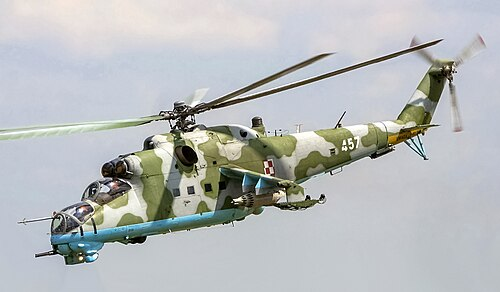
\includegraphics{../images/lotnictwo/mi-24_1.jpg}
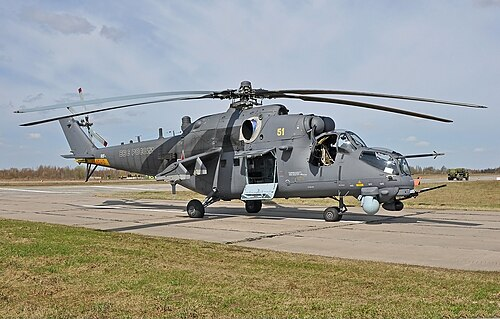
\includegraphics{../images/lotnictwo/mi-24_2.jpg}

\begin{center}\rule{0.5\linewidth}{0.5pt}\end{center}

\subsection{Opis}\label{opis-54}

Mi-24 to radzieckie ciężkie wojskowe śmigłowce szturmowo-transportowe,
opracowane przez biuro Michaiła Mila w latach 60. XX wieku. Koncepcja
była nowatorska: połączenie potężnego śmigłowca uderzeniowego z
zdolnością transportu ośmiu żołnierzy desantu --- stąd określenie
``latający czołg'' lub ``latający IFV''. Chrzest bojowy przeszedł
podczas Ogadenu (1977--78), jednak prawdziwą sławę zyskał w Afganistanie
w latach 1979--1989, gdzie za waleczność i odporność na ostrzał
Mudżahedini nadali mu przezwisko ``Szatan'' (Shaitan-Arba). Do dziś
służy w wojskach rosyjskich i jest szeroko stosowany w konflikcie na
Ukrainie.

\subsection{Dane techniczne}\label{dane-techniczne-54}

\begin{longtable}[]{@{}
  >{\raggedright\arraybackslash}p{(\columnwidth - 2\tabcolsep) * \real{0.5263}}
  >{\raggedright\arraybackslash}p{(\columnwidth - 2\tabcolsep) * \real{0.4737}}@{}}
\toprule\noalign{}
\begin{minipage}[b]{\linewidth}\raggedright
Parametr
\end{minipage} & \begin{minipage}[b]{\linewidth}\raggedright
Wartość
\end{minipage} \\
\midrule\noalign{}
\endhead
\bottomrule\noalign{}
\endlastfoot
Typ & Śmigłowiec szturmowo-transportowy \\
Kraj produkcji & ZSRR / Rosja \\
Rok wprowadzenia & 1972 \\
Masa startowa & \textasciitilde11 500 kg (maks.) \\
Długość & 17,51 m (kadłub) \\
Średnica rotora & 17,30 m (pięciołopatowy) \\
Uzbrojenie & Działko dwulufowe 12,7 mm lub 23 mm GSh-23L; rakiety
S-5/S-8/S-24; ppk 9M114 Sztorm / 9M120 Ataka; bomby \\
Silnik & 2 × Klimov TV3-117 (turbowałowy, ok. 1640 kW każdy) \\
Prędkość maks. & 335 km/h (rekordowa 368 km/h) \\
Pułap & 4 500 m (dynamiczny ok. 4 950 m) \\
Zasięg & 450 km (bojowy); 1 000 km (z dodatkowymi zbiornikami) \\
Załoga & 2 os. + do 8 żołnierzy desantu \\
\end{longtable}

\subsection{Charakterystyczne cechy
rozpoznawcze}\label{charakterystyczne-cechy-rozpoznawcze-54}

\begin{quote}
Jak odróżnić Mi-24 od innych śmigłowców:
\end{quote}

\begin{itemize}
\tightlist
\item
  \textbf{Charakterystyczny ``garb'' kabiny:} Dwuosobowa kabina z
  siedzeniami w układzie tandem (strzelec z przodu, pilot wyżej z tyłu)
  --- tworzy wyraźnie owalny, wypukły kształt dzioba widoczny z
  odległości.
\item
  \textbf{Skrzydła boczne (sponsony):} Mi-24 jako jedyny spośród
  rosyjskich śmigłowców bojowych posiada krótkie, przykabinowe skrzydła
  nośne z twardymi punktami uzbrojenia --- wyglądają jak małe, odchylone
  w dół skrzydełka po obu stronach kadłuba.
\item
  \textbf{Ogromny, zamknięty przedział desantowy:} Kadłub jest znacząco
  szerszy i wyższy niż u Mi-28 czy Ka-52 --- widać to szczególnie od
  tyłu i z boku; śmigłowiec wygląda ``pulchniej''.
\item
  \textbf{Pięciołopatowy rotor główny:} Wyraźnie duży, pięciołopatowy
  rotor o średnicy 17,3 m widoczny z góry, zazwyczaj z
  charakterystycznym świstem.
\item
  \textbf{Trójkołowe podwozie chowane:} Większość wariantów posiada
  chowane podwozie kołowe --- w locie widać schowany do kadłuba układ
  podwozia, co odróżnia go od wielu zachodnich śmigłowców z płozami.
\item
  \textbf{Gondola uzbrojenia pod dziobem:} Zależnie od wariantu ---
  obrotowa wieżyczka z działkiem (Mi-24V/P) lub stałe działko 30 mm
  (Mi-24P) umieszczone wyraźnie po prawej stronie dzioba, nadając mu
  asymetryczny wygląd.
\end{itemize}

\subsection{Ciekawostka}\label{ciekawostka-54}

\begin{quote}
Mi-24 jest jedynym na świecie śmigłowcem bojowym, który w 1978 roku
oficjalnie pobił rekord prędkości dla śmigłowców --- specjalnie
zmodyfikowany egzemplarz Mi-24A osiągnął 368,4 km/h, a rekord ten przez
wiele lat był oficjalnie homologowany przez FAI.
\end{quote}

\section{Mi-28 Havoc}\label{mi-28-havoc}

\subsubsection{Mil Mi-28N Night Hunter \textbar{} Миль Ми-28Н «Ночной
охотник»}\label{mil-mi-28n-night-hunter-ux43cux438ux43bux44c-ux43cux438-28ux43d-ux43dux43eux447ux43dux43eux439-ux43eux445ux43eux442ux43dux438ux43a}

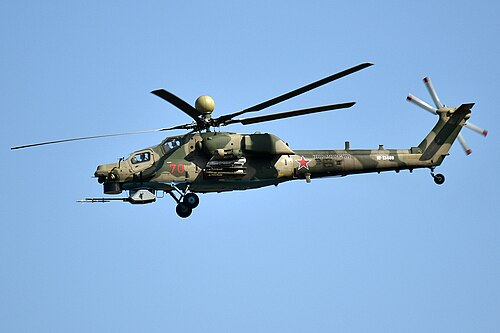
\includegraphics{../images/lotnictwo/mi-28_1.jpg}
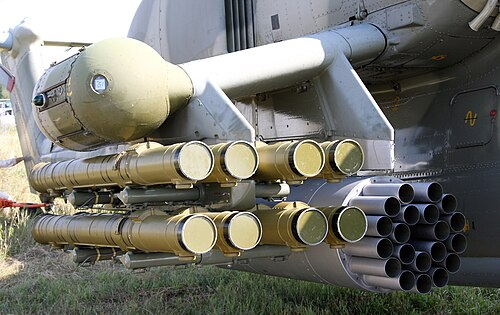
\includegraphics{../images/lotnictwo/mi-28_2.jpg}

\begin{center}\rule{0.5\linewidth}{0.5pt}\end{center}

\subsection{Opis}\label{opis-55}

Mi-28 to rosyjski śmigłowiec szturmowy czwartej generacji, opracowany
przez biuro Mila od 1980 roku jako odpowiedź na amerykański AH-64
Apache. W odróżnieniu od swojego poprzednika Mi-24, jest to
wyspecjalizowana maszyna uderzeniowa bez przedziału desantowego --- cały
nacisk położono na zdolności bojowe i przeżywalność. Wariant Mi-28N
``Nocny Myśliwy'' (Nocnoj Ochotnik) wyposażono w radar nad wirnikiem i
systemy noktowizyjne, co umożliwia operacje nocne. Śmigłowiec wszedł do
służby operacyjnej dopiero w 2009 roku i szybko stał się jedną z
głównych maszyn bojowych Sił Powietrzno-Kosmicznych Rosji, uczestnicząc
w operacjach w Syrii i na Ukrainie.

\subsection{Dane techniczne}\label{dane-techniczne-55}

\begin{longtable}[]{@{}
  >{\raggedright\arraybackslash}p{(\columnwidth - 2\tabcolsep) * \real{0.5263}}
  >{\raggedright\arraybackslash}p{(\columnwidth - 2\tabcolsep) * \real{0.4737}}@{}}
\toprule\noalign{}
\begin{minipage}[b]{\linewidth}\raggedright
Parametr
\end{minipage} & \begin{minipage}[b]{\linewidth}\raggedright
Wartość
\end{minipage} \\
\midrule\noalign{}
\endhead
\bottomrule\noalign{}
\endlastfoot
Typ & Śmigłowiec szturmowy \\
Kraj produkcji & Rosja \\
Rok wprowadzenia & 2009 \\
Masa startowa & 11 500 kg (maks.) \\
Długość & 17,01 m (kadłub) \\
Średnica rotora & 17,20 m (pięciołopatowy) \\
Uzbrojenie & Działko 2A42 kalibru 30 mm; ppk 9M120 Ataka (do 16 szt.);
rakiety S-8, S-13; zasobniki NARS \\
Silnik & 2 × Klimov VK-2500 (turbowałowy, 1 636 kW każdy) \\
Prędkość maks. & 320 km/h \\
Pułap & 5 700 m \\
Zasięg & 435 km \\
Załoga & 2 os. (pilot i operator uzbrojenia) \\
\end{longtable}

\subsection{Charakterystyczne cechy
rozpoznawcze}\label{charakterystyczne-cechy-rozpoznawcze-55}

\begin{quote}
Jak odróżnić Mi-28 od Mi-24 i Ka-52:
\end{quote}

\begin{itemize}
\tightlist
\item
  \textbf{Smukły, wrzecionowaty kadłub:} Mi-28 nie ma przedziału
  desantowego --- kadłub jest znacznie węższy i bardziej aerodynamiczny
  niż u Mi-24; profil boczny przypomina wydłużoną kroplę z wyraźnie
  oddzielonymi kabinami.
\item
  \textbf{Kopuła radarowa nad wirnikiem (Mi-28N):} Charakterystyczna
  sferyczna lub owalna kulista osłona radaru umieszczona ponad
  płaszczyzną wirnika głównego --- to najbardziej rozpoznawalny element,
  odróżniający Mi-28N od wszystkich innych rosyjskich śmigłowców.
\item
  \textbf{Tandemowe kabiny z wyraźnym ``schodkiem'':} Kabina pilota (z
  tyłu, wyżej) i operatora uzbrojenia (z przodu, niżej) tworzą wyraźny
  schodkowy profil --- bardziej kwadratowe i ostrzejsze niż zaokrąglony
  ``garb'' Mi-24.
\item
  \textbf{Brak skrzydeł nośnych w stylu Mi-24:} Sponsony z uzbrojeniem
  są krótsze i bardziej prostopadłe do kadłuba, bez charakterystycznego
  odchylenia w dół typowego dla Mi-24.
\item
  \textbf{Działko 30 mm w ruchomej wieżyczce poddziobowej:} Kątnisty
  montaż działka pod przednią częścią kadłuba --- przemieszcza się
  widocznie w bok podczas celowania, co jest dobrze widoczne na
  zdjęciach i nagraniach.
\item
  \textbf{Niskie, sztywne podwozie kołowe (niechowane):} Mi-28 ma stałe
  podwozie kołowe z wyraźną osią główną i kółkiem ogonowym --- w locie
  brak jakichkolwiek ruchomych elementów podwozia pod kadłubem.
\end{itemize}

\subsection{Ciekawostka}\label{ciekawostka-55}

\begin{quote}
Pomimo oficjalnego przyjęcia do służby dopiero w 2009 roku, Mi-28 latał
jako prototyp już od 1982 roku --- przez niemal 27 lat trwały testy,
modyfikacje i rywalizacja z Ka-50, zanim śmigłowiec trafił do linii
bojowych. To jeden z najdłuższych procesów wdrożeniowych w historii
rosyjskiego lotnictwa wojskowego.
\end{quote}

\section{Ka-52 Aligator}\label{ka-52-aligator}

\subsubsection{Kamov Ka-52 Alligator \textbar{} Камов Ка-52
«Аллигатор»}\label{kamov-ka-52-alligator-ux43aux430ux43cux43eux432-ux43aux430-52-ux430ux43bux43bux438ux433ux430ux442ux43eux440}

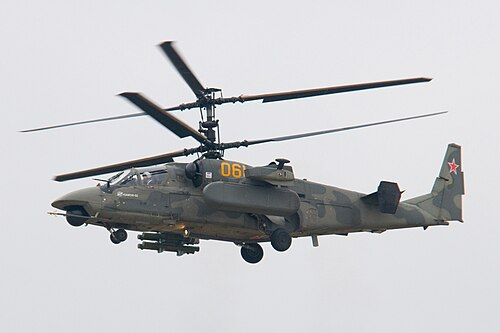
\includegraphics{../images/lotnictwo/ka-52_1.jpg}
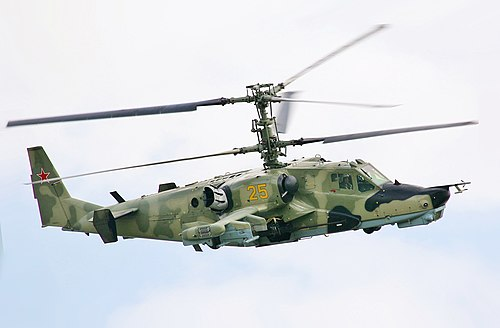
\includegraphics{../images/lotnictwo/ka-52_2.jpg}

\begin{center}\rule{0.5\linewidth}{0.5pt}\end{center}

\subsection{Opis}\label{opis-56}

Ka-52 ``Aligator'' to rosyjski śmigłowiec szturmowy dwumiejscowy,
opracowany przez biuro Kamowa jako rozwinięcie jednosobowego Ka-50
``Czarny Rekin''. Jego najważniejszą cechą konstrukcyjną jest układ
dwóch współosiowych wirników przeciwbieżnych --- całkowicie eliminujący
potrzebę wirnika ogonowego. Dzięki temu Ka-52 jest wyjątkowo zwrotny i
może wykonywać manewry niemożliwe dla śmigłowców z klasycznym układem
napędu. Śmigłowiec wszedł do służby w 2011 roku i jest szeroko stosowany
przez Siły Powietrzno-Kosmiczne Rosji --- brał udział w operacji w Syrii
oraz w inwazji na Ukrainę od 2022 roku, gdzie poniósł znaczne straty,
głównie od zachodnich zestawów rakietowych MANPADS i systemów
przeciwlotniczych.

\subsection{Dane techniczne}\label{dane-techniczne-56}

\begin{longtable}[]{@{}
  >{\raggedright\arraybackslash}p{(\columnwidth - 2\tabcolsep) * \real{0.5263}}
  >{\raggedright\arraybackslash}p{(\columnwidth - 2\tabcolsep) * \real{0.4737}}@{}}
\toprule\noalign{}
\begin{minipage}[b]{\linewidth}\raggedright
Parametr
\end{minipage} & \begin{minipage}[b]{\linewidth}\raggedright
Wartość
\end{minipage} \\
\midrule\noalign{}
\endhead
\bottomrule\noalign{}
\endlastfoot
Typ & Śmigłowiec szturmowy \\
Kraj produkcji & Rosja \\
Rok wprowadzenia & 2011 \\
Masa startowa & 10 800 kg (maks.) \\
Długość & 13,50 m (kadłub bez wirników) \\
Średnica rotorów & 14,50 m (dwa wirniki współosiowe) \\
Uzbrojenie & Działko 2A42 kalibru 30 mm (ruchoma wieżyczka); ppk 9M120
Ataka, Ch-25ML; rakiety S-8, S-13; bomby \\
Silnik & 2 × Klimov VK-2500 (turbowałowy, 1 800 kW każdy) \\
Prędkość maks. & 315 km/h \\
Pułap & 5 500 m \\
Zasięg & 460 km (bojowy) \\
Załoga & 2 os. (pilot i operator uzbrojenia, fotele wyrzucane) \\
\end{longtable}

\subsection{Charakterystyczne cechy
rozpoznawcze}\label{charakterystyczne-cechy-rozpoznawcze-56}

\begin{quote}
Jak odróżnić Ka-52 od Mi-28 i Mi-24:
\end{quote}

\begin{itemize}
\tightlist
\item
  \textbf{Dwa współosiowe wirniki przeciwbieżne --- brak wirnika
  ogonowego:} To absolutnie unikatowa i natychmiast widoczna cecha.
  Ka-52 nie ma wirnika ogonowego --- zamiast niego dwa pięciołopatowe
  wirniki kręcą się jeden nad drugim w przeciwnych kierunkach. Z każdej
  strony i z przodu widać ``podwójny dysk'' wirnikowy.
\item
  \textbf{Belka ogonowa bez wirnika bocznego:} Ogon Ka-52 kończy się
  płetwą pionową bez dodatkowego wirnika --- charakterystyczny ``goły''
  ogon ze statecznikami poziomymi i pionowym, zamiast typowej łopatki
  wirnika ogonowego.
\item
  \textbf{Szerokie, płaskie fotele obok siebie (side-by-side):} W
  odróżnieniu od Mi-28 i Mi-24, obaj członkowie załogi siedzą obok
  siebie w tej samej kabinie --- stąd wyraźnie szerszy nos śmigłowca,
  widoczny od przodu jako dwuszybowa kokpit z boku na bok.
\item
  \textbf{Kompaktowy, ``przysadzisty'' kadłub:} Ka-52 jest krótszy i
  bardziej masywny niż Mi-28 --- proporcje są bardziej kwadratowe, bez
  długiej smukłej belki dziobowej.
\item
  \textbf{Fotele wyrzucane katapultą:} Ka-52 i Ka-50 to jedyne seryjnie
  produkowane śmigłowce z wyrzucanymi fotelami ratunkowymi ---
  niewielkie ładunki wybuchowe na górze wirników odrywają łopaty przed
  wyrzuceniem pilotów.
\item
  \textbf{Działko 30 mm z prawej strony nosa:} Ruchoma wieżyczka z
  działkiem 2A42 zamontowana jest po prawej stronie przedniej części
  kadłuba --- asymetryczne umiejscowienie jest dobrze widoczne z przodu
  i z boku.
\end{itemize}

\subsection{Ciekawostka}\label{ciekawostka-56}

\begin{quote}
Ka-52 (podobnie jak Ka-50) jest jedynym śmigłowcem bojowym na świecie
produkowanym seryjnie z fotelami wyrzucanymi --- systemu K-37-800. Przed
katapultowaniem specjalne ładunki pirotechniczne detonują łopaty
wirników, aby nie zabiły pilota. Cały proces zajmuje ułamek sekundy.
\end{quote}

\section{Su-25 Gracz}\label{su-25-gracz}

\subsubsection{Sukhoi Su-25 Frogfoot \textbar{} Сухой Су-25
«Грач»}\label{sukhoi-su-25-frogfoot-ux441ux443ux445ux43eux439-ux441ux443-25-ux433ux440ux430ux447}

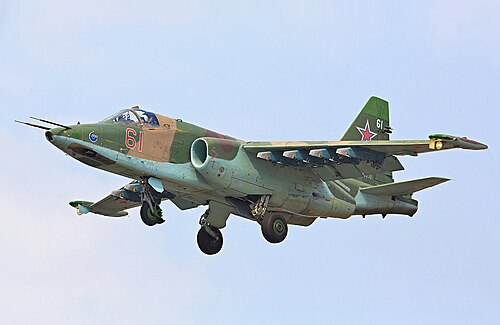
\includegraphics{../images/lotnictwo/su-25_1.jpg}
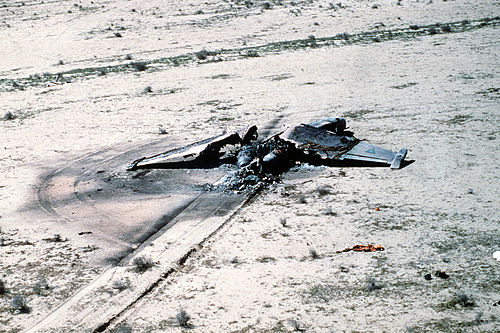
\includegraphics{../images/lotnictwo/su-25_2.jpg}

\begin{center}\rule{0.5\linewidth}{0.5pt}\end{center}

\subsection{Opis}\label{opis-57}

Su-25 ``Gracz'' (ros. Грач --- kawka) to radziecki/rosyjski samolot
szturmowy bliskiego wsparcia, zaprojektowany specjalnie do
bezpośredniego wsparcia wojsk lądowych w strefie kontaktu. Opracowany od
końca lat 60., po raz pierwszy oblatany 22 lutego 1975 roku, wszedł do
służby w 1981 roku i natychmiast trafił do Afganistanu, gdzie sprawdził
się znakomicie. Zaprojektowany z myślą o przeżywalności: kokpit pilota
chroniony jest tytanową ``wanną'' odporną na ogień karabinów maszynowych
i odłamki; silniki otoczone są stalowymi przegrodami. Samolot
uczestniczył w niemal każdym konflikcie zbrojnym z udziałem państw
postsowieckich, od Czeczenii przez Gruzję aż po Ukrainę 2022+, gdzie
obie strony używają Su-25 do szturmowania pozycji naziemnych.

\subsection{Dane techniczne}\label{dane-techniczne-57}

\begin{longtable}[]{@{}
  >{\raggedright\arraybackslash}p{(\columnwidth - 2\tabcolsep) * \real{0.5263}}
  >{\raggedright\arraybackslash}p{(\columnwidth - 2\tabcolsep) * \real{0.4737}}@{}}
\toprule\noalign{}
\begin{minipage}[b]{\linewidth}\raggedright
Parametr
\end{minipage} & \begin{minipage}[b]{\linewidth}\raggedright
Wartość
\end{minipage} \\
\midrule\noalign{}
\endhead
\bottomrule\noalign{}
\endlastfoot
Typ & Samolot szturmowy (CAS) \\
Kraj produkcji & ZSRR / Rosja \\
Rok wprowadzenia & 1981 \\
Masa startowa & 19 300 kg (maks.) \\
Długość & 15,53 m \\
Rozpiętość skrzydeł & 14,36 m \\
Uzbrojenie & Działko 30 mm GSh-30-2 (250 naboi); do 4 000 kg bomb,
rakiet S-5/S-8/S-24/Ch-25, zasobników działek; ppk Ch-29 \\
Silnik & 2 × Tumanski R-195 (odrzutowy, 44,18 kN każdy) \\
Prędkość maks. & 975 km/h \\
Pułap & 7 000 m \\
Zasięg & 750 km (bojowy) \\
Załoga & 1 os. \\
\end{longtable}

\subsection{Charakterystyczne cechy
rozpoznawcze}\label{charakterystyczne-cechy-rozpoznawcze-57}

\begin{quote}
Jak odróżnić Su-25 od innych samolotów szturmowych:
\end{quote}

\begin{itemize}
\tightlist
\item
  \textbf{Mocno podwieszony, wysoko osadzony płat wysoki:} Skrzydła
  osadzone są wysoko na kadłubie, w konfiguracji niemal średniopłata ---
  z przodu widać prosty trapezowy profil skrzydła z lekkim skosem przy
  krawędzi natarcia i bardzo wyraźnymi węzłami podwieszeń (do 10
  pylonów).
\item
  \textbf{Dwa silniki odrzutowe po bokach kadłuba --- ``paczki''
  gondol:} Su-25 ma dwa silniki umieszczone w cylindrycznych gondolach
  po bokach tylnej części kadłuba (nie w kadłubie). Z tyłu i z boku
  widać wyraźnie dwie okrągłe dysze wyrzutu spalin symetrycznie po obu
  stronach ogona.
\item
  \textbf{Charakterystyczna ``krótka i przysadzista'' sylwetka:} Samolot
  jest relatywnie krótki i chudy --- proporcje kadłuba (okrągły
  przekrój, krótkie skrzydła) nadają mu sylwetkę niemal ciężkiej rury z
  małymi skrzydłami.
\item
  \textbf{Płaski nos z ostrą krawędzią --- bez radaru:} Dziób Su-25 jest
  zaostrzony i stosunkowo płaski, bez charakterystycznej stożkowej
  osłony radarowej --- to samolot szturmowy, nie myśliwiec, więc nos
  jest prosty.
\item
  \textbf{Duże spojlery i klapy na skrzydłach:} Z bliska lub na
  zdjęciach lądowania widać rozbudowany system klap i spoilerów
  zajmujący dużą część tylnej krawędzi skrzydła --- potrzebny do
  operowania z krótkich pasów.
\item
  \textbf{Tytanowy ``kocioł'' w okolicach kabiny:} Grube opancerzenie
  wokół kokpitu jest widoczne jako wyraźnie grubsza sekcja kadłuba tuż
  za dziobem --- Su-25 wygląda ``bardziej mięsisty'' w środkowej części
  niż typowy odrzutowiec.
\end{itemize}

\subsection{Ciekawostka}\label{ciekawostka-57}

\begin{quote}
Opancerzenie kabiny Su-25 składa się z tytanowej ``wanny'' o grubości 24
mm i ważącej samo w sobie 595 kg --- stanowi to ok. 7\% pustej masy
samolotu. Wanna chroni pilota ze wszystkich stron i od dołu przed
ostrzałem z broni strzeleckiej i odłamkami artylerii przeciwlotniczej.
\end{quote}

\section{Su-27 Flanker}\label{su-27-flanker}

\subsubsection{Sukhoi Su-27 Flanker \textbar{} Сухой
Су-27}\label{sukhoi-su-27-flanker-ux441ux443ux445ux43eux439-ux441ux443-27}

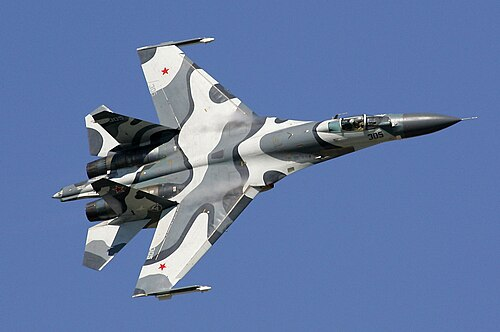
\includegraphics{../images/lotnictwo/su-27_1.jpg}
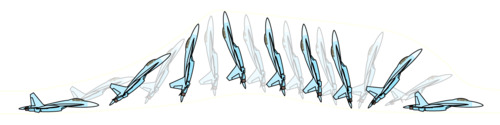
\includegraphics{../images/lotnictwo/su-27_2.jpg}

\begin{center}\rule{0.5\linewidth}{0.5pt}\end{center}

\subsection{Opis}\label{opis-58}

Su-27 ``Flanker'' to radziecki/rosyjski myśliwiec czwartej generacji,
opracowany jako odpowiedź na amerykańskie F-15 Eagle. Zaprojektowany
przez biuro Suchoja w latach 70., wszedł do służby w 1985 roku jako
podstawowy myśliwiec superiorności powietrznej radzieckich sił obrony
powietrznej. Charakteryzuje się wyjątkową zwrotnością, zasięgiem (ponad
3 500 km bez doładowania) i dużą ładownością uzbrojenia. Su-27 dał
początek całej rodzinie maszyn --- Su-30, Su-33, Su-34, Su-35 --- które
do dziś stanowią kręgosłup rosyjskiego lotnictwa bojowego. W konflikcie
ukraińskim zarówno Rosja, jak i Ukraina używają różnych wariantów tej
rodziny.

\subsection{Dane techniczne}\label{dane-techniczne-58}

\begin{longtable}[]{@{}
  >{\raggedright\arraybackslash}p{(\columnwidth - 2\tabcolsep) * \real{0.5263}}
  >{\raggedright\arraybackslash}p{(\columnwidth - 2\tabcolsep) * \real{0.4737}}@{}}
\toprule\noalign{}
\begin{minipage}[b]{\linewidth}\raggedright
Parametr
\end{minipage} & \begin{minipage}[b]{\linewidth}\raggedright
Wartość
\end{minipage} \\
\midrule\noalign{}
\endhead
\bottomrule\noalign{}
\endlastfoot
Typ & Myśliwiec superiorności powietrznej \\
Kraj produkcji & ZSRR / Rosja \\
Rok wprowadzenia & 1985 \\
Masa startowa & 33 000 kg (maks.) \\
Długość & 21,94 m \\
Rozpiętość skrzydeł & 14,70 m \\
Uzbrojenie & Działko 30 mm GSh-30-1 (150 naboi); do 10 rakiet
powietrze--powietrze R-73, R-27, R-77; możliwość przenoszenia bomb i
rakiet powietrze--ziemia \\
Silnik & 2 × Saturn AL-31F (turboodrzutowy z dopalaczem, 2 × 122,6 kN z
dopalaczem) \\
Prędkość maks. & \textasciitilde2 500 km/h (Mach 2,35) \\
Pułap & 19 000 m \\
Zasięg & 3 530 km (bez zbiorników dodatkowych) \\
Załoga & 1 os. \\
\end{longtable}

\subsection{Charakterystyczne cechy
rozpoznawcze}\label{charakterystyczne-cechy-rozpoznawcze-58}

\begin{quote}
Jak odróżnić Su-27 od MiG-29 i zachodnich myśliwców:
\end{quote}

\begin{itemize}
\tightlist
\item
  \textbf{Podwójne stateczniki pionowe (dublowane ogony):} Su-27 ma dwa
  pionowe stateczniki --- jeden nad każdym silnikiem. Ten
  charakterystyczny ``podwójny ogon'' jest widoczny z każdego kierunku i
  natychmiast odróżnia go od większości myśliwców z jednym usterzeniem
  pionowym.
\item
  \textbf{Bardzo długi, smukły kadłub z ``nacelle'' silników:} Dwie
  gondole silnikowe biegną wzdłuż całej tylnej połowy kadłuba, widocznie
  wystając za linię skrzydła --- z dołu i z tyłu widać charakterystyczny
  ``grzebień'' dwóch równoległych wyrzutni dyszy.
\item
  \textbf{Charakterystyczny profil nosa z dużą radome:} Długi,
  zaostrzony nos z wyraźnie zaokrągloną osłoną radaru (radome) zajmującą
  ok. jednej trzeciej długości dzioba --- wyraźnie większy i bardziej
  dominujący niż np. u MiG-29.
\item
  \textbf{Skrzydła typu ``odwróconego delta'' z LERX:} Duże, trapezowe
  skrzydła z mocno zaciągniętym skosem przy nasadzie (LERX --- leading
  edge root extension) tworzą charakterystyczny esowaty kształt
  przedniej krawędzi widziany z góry lub z przodu.
\item
  \textbf{Wloty powietrza z przodu pod kadłubem:} Dwa prostokątne wloty
  powietrza umieszczone symetrycznie pod kadłubem między silnikami a
  krawędzią natarcia skrzydła --- z przodu widać wyraźnie dwa
  ``nozdrza'' po bokach dolnej części kadłuba.
\item
  \textbf{Duże rozmiary --- wyraźnie większy od MiG-29:} Su-27 jest dużo
  większy od MiG-29 (o ok. 6 m dłuższy) --- ta różnica skali jest
  widoczna na lotnisku lub w porównaniu do innych samolotów obok.
\end{itemize}

\subsection{Ciekawostka}\label{ciekawostka-58}

\begin{quote}
Na pokazach lotniczych Su-27 zasłynął manewrem ``kobra Pugaczowa'' ---
pilotowanym przez Wiktora Pugaczowa na Paris Air Show w 1989 roku.
Samolot unosi dziób pionowo (a nawet odchyla się do tyłu), zwalnia
niemal do zera i wraca do lotu poziomego, zachowując w przybliżeniu
trajektorię poziomą. Żaden zachodni myśliwiec tamtej epoki nie był w
stanie wykonać tego manewru, co wywarło ogromne wrażenie na zachodniej
publiczności i analitykach wojskowych.
\end{quote}

\section{Karabin szturmowy AK-74}\label{karabin-szturmowy-ak-74}

\subsubsection{AK-74 Assault Rifle \textbar{}
АК-74}\label{ak-74-assault-rifle-ux430ux43a-74}

\begin{figure}
\centering
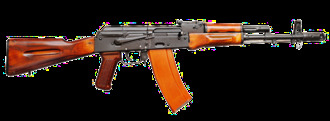
\includegraphics{../images/karabiny/ak-74_1.jpg}
\caption{AK-74 --- widok z lewej strony}
\end{figure}

\begin{center}\rule{0.5\linewidth}{0.5pt}\end{center}

\subsection{Opis}\label{opis-59}

AK-74 to radziecki karabin szturmowy zaprojektowany przez Michaiła
Kałasznikowa w 1974 roku jako następca AKM, przystosowany do nowego
naboju 5,45×39 mm o mniejszym kalibrze i wyższej prędkości wylotowej.
Mniejszy kaliber zapewnił żołnierzowi możliwość niesienia większego
zapasu amunicji przy tej samej masie, a wysoka prędkość pocisku
(880--900 m/s) poprawiła skuteczność rażenia. AK-74 po raz pierwszy
trafił do walki w Afganistanie w 1979 roku. Zmodernizowana wersja AK-74M
z 1991 roku, z plastikową kolbą składaną i szyną Picatinny, jest do dziś
podstawowym karabinem piechoty rosyjskiej. Posłużył jako wzorzec dla
całej rodziny AK-100 i współczesnych AK-12/AK-15.

\subsection{Dane techniczne}\label{dane-techniczne-59}

\begin{longtable}[]{@{}ll@{}}
\toprule\noalign{}
Parametr & Wartość \\
\midrule\noalign{}
\endhead
\bottomrule\noalign{}
\endlastfoot
Typ & Karabin szturmowy \\
Kraj produkcji & ZSRR / Rosja \\
Rok wprowadzenia & 1974 \\
Kaliber & 5,45×39 mm \\
Długość (kolba rozłożona) & 943 mm \\
Długość lufy & 415 mm \\
Masa (bez magazynka) & 3,07 kg \\
Pojemność magazynka & 30 nabojów (standardowy) \\
Szybkostrzelność & 650 strz./min \\
Prędkość wylotowa & 880--900 m/s \\
Skuteczny zasięg & 500 m (cel punktowy) / 800 m (cel grupowy) \\
\end{longtable}

\subsection{Charakterystyczne cechy
rozpoznawcze}\label{charakterystyczne-cechy-rozpoznawcze-59}

\begin{quote}
Jak odróżnić AK-74 od AKM i innych Kałasznikowów:
\end{quote}

\begin{itemize}
\tightlist
\item
  \textbf{Charakterystyczny hamulec wylotowy z bocznym otworem:}
  unikalny cylindryczny hamulec kompensator z poprzecznym prostokątnym
  oknem po lewej stronie --- żaden inny AK nie ma identycznego --- to
  natychmiastowy identyfikator AK-74
\item
  \textbf{Pomarańczowo-brązowy magazynek z żeberkami:} standardowy
  magazynek AK-74 jest wykonany z pomarańczowego lub brązowego bakelitu
  z poprzecznymi żeberkami; magazynki AKM są stalowe lub czarne
  plastikowe
\item
  \textbf{Smuklejsza lufa niż AKM:} kaliber 5,45 mm daje AK-74 wyraźnie
  cieńszą lufę niż AKM (7,62 mm) --- widoczne przy porównaniu obu broni
\item
  \textbf{Wycięcie w zamku (charakterystyczne):} zamek AK-74 ma nieco
  inne proporcje niż AKM; pudło zamkowe jest identyczne, ale detale
  różnią się od pierwszego wejrzenia
\item
  \textbf{AK-74M: składana czarna plastikowa kolba:} wersja M ma
  charakterystyczną czarną kolbę składaną w bok (nie jak AKM ---
  drewniana lub składana ku dołowi) z charakterystycznym blokadą
\item
  \textbf{Krótszy niż SVD, dłuższy niż AKS-74U:} proporcje karabinu są
  pośrednie; nie tak długi jak SVD, nie tak krótki jak AKS-74U ---
  pomocne przy identyfikacji z odległości
\end{itemize}

\subsection{Ciekawostka}\label{ciekawostka-59}

\begin{quote}
Pocisk 5,45×39 mm AK-74 był przez zachodnie służby wywiadowcze nazywany
``Poison Bullet'' (Trująca Kula) --- nie z powodu substancji
chemicznych, ale dlatego że po trafieniu w ciało pocisk traci stabilność
i zaczyna się obracać w tkankach, powodując nieproporcjonalnie duże rany
w stosunku do małego kalibru. Właściwość ta była w sowieckim projekcie
zamierzona i od razu wzbudziła kontrowersje podczas debat o Konwencji
Haskiej.
\end{quote}

\section{Skrócony karabin szturmowy
AKS-74U}\label{skruxf3cony-karabin-szturmowy-aks-74u}

\subsubsection{AKS-74U Carbine \textbar{} АКС-74У
(«Ксюха»)}\label{aks-74u-carbine-ux430ux43aux441-74ux443-ux43aux441ux44eux445ux430}

\begin{center}\rule{0.5\linewidth}{0.5pt}\end{center}

\begin{figure}
\centering
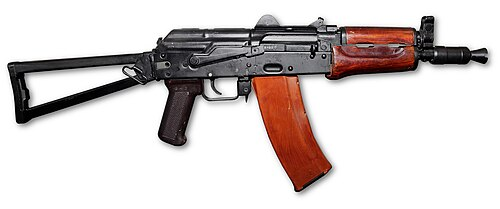
\includegraphics{../images/karabiny/aks-74u_1.jpg}
\caption{AKS-74U --- skrócony karabin szturmowy}
\end{figure}

\subsection{Opis}\label{opis-60}

AKS-74U (potocznie: „Ksyucha'') to radziecka skrócona wersja karabinu
AKS-74 z odchylaną kolbą i krótką lufą (212 mm zamiast 415 mm),
zaprojektowana w 1977 roku dla służb specjalnych, kierowców pojazdów
bojowych, obsługi sprzętu artyleryjskiego i sił powietrznodesantowych.
Mała masa (\textasciitilde2,7 kg) i kompaktowe wymiary (490 mm z kolbą
złożoną) czynią ją idealną bronią osobistą tam, gdzie pełnowymiarowy
karabin byłby niewygodny. Ceną za mały rozmiar jest znacznie zmniejszona
celność i zasięg skuteczny (200 m zamiast 500 m) oraz wyraźnie
głośniejszy huk i mocniejszy płomień wylotowy. AKS-74U była standardową
bronią radzieckich i rosyjskich oddziałów specjalnych przez dekady.

\subsection{Dane techniczne}\label{dane-techniczne-60}

\begin{longtable}[]{@{}ll@{}}
\toprule\noalign{}
Parametr & Wartość \\
\midrule\noalign{}
\endhead
\bottomrule\noalign{}
\endlastfoot
Typ & Skrócony karabin szturmowy (PDW/karabin) \\
Kraj produkcji & ZSRR / Rosja \\
Rok wprowadzenia & 1979 \\
Kaliber & 5,45×39 mm \\
Długość (kolba rozłożona) & 735 mm \\
Długość (kolba złożona) & 490 mm \\
Długość lufy & 212 mm \\
Masa (bez magazynka) & 2,7 kg \\
Pojemność magazynka & 30 nabojów \\
Szybkostrzelność & 700 strz./min \\
Skuteczny zasięg & 200 m \\
\end{longtable}

\subsection{Charakterystyczne cechy
rozpoznawcze}\label{charakterystyczne-cechy-rozpoznawcze-60}

\begin{quote}
Jak odróżnić AKS-74U od AK-74 i innych Kałasznikowów:
\end{quote}

\begin{itemize}
\tightlist
\item
  \textbf{Bardzo krótka lufa z dużym rozbudowanym tłumikiem
  gazowym/kompensatorem:} na krótkiej lufie widnieje charakterystyczny
  duży cylindryczny kompensator wylotowy --- nieproporcjonalnie duży do
  długości lufy; żaden inny AK nie wygląda tak
\item
  \textbf{Boczna składana metalowa kolba (na lewą stronę):} kolba
  AKS-74U składa się na lewą stronę i jest metalowa, kratownicowa ---
  wyraźnie różna od plastikowej kolby AK-74M
\item
  \textbf{Skrócone łoże --- rączkę pistoletową widać blisko komory
  zamkowej:} łoże jest bardzo krótkie, a chwyt pistoletowy jest znacznie
  bliżej komory zamkowej niż w standardowym AK-74 --- proporcje są
  wyraźnie inne
\item
  \textbf{Mała, prosta muszka bez podstawy gazowej na lufie:} gazownik
  AKS-74U jest tuż przy komorze, a muszka stoi na krótkim bloku przy
  komórze wylotowej --- inny układ niż w pełnowymiarowym karabinie
\item
  \textbf{Wyraźnie krótszy od jakiegokolwiek pełnowymiarowego AK:} z
  kolbą złożoną AKS-74U wygląda jak pistolet maszynowy --- jest krótszy
  niż lufa standardowego AK-74
\item
  \textbf{Magazynek 5,45 mm (pomarańczowy lub brązowy) --- tak jak
  AK-74:} magazynek jest identyczny jak w AK-74, co odróżnia od
  skróconego AKS-74U kalibru 7,62 (AKS)
\end{itemize}

\subsection{Ciekawostka}\label{ciekawostka-60}

\begin{quote}
AKS-74U zyskała przydomek ``Ksyucha'' (ros. zdrobnienie imienia Ksenija)
od rosyjskich żołnierzy --- według legendy dlatego, że jest ``kapryśna
jak kobieta'' i często powoduje zacięcia przy intensywnej strzelaniu ze
względu na bardzo krótki cykl pracy gazów. Afgańscy mudżahedini
zdobywając AKS-74U na sowieckich żołnierzach nazywali ją ``małym
karabin'' i traktowali jako szczególny łup --- ze względu na rozmiary
łatwiejszy do ukrycia pod ubraniem niż pełny AK.
\end{quote}

\section{Karabin szturmowy AKM}\label{karabin-szturmowy-akm}

\subsubsection{AKM Assault Rifle \textbar{} АКМ (Автомат Калашникова
Модернизированный)}\label{akm-assault-rifle-ux430ux43aux43c-ux430ux432ux442ux43eux43cux430ux442-ux43aux430ux43bux430ux448ux43dux438ux43aux43eux432ux430-ux43cux43eux434ux435ux440ux43dux438ux437ux438ux440ux43eux432ux430ux43dux43dux44bux439}

\begin{figure}
\centering
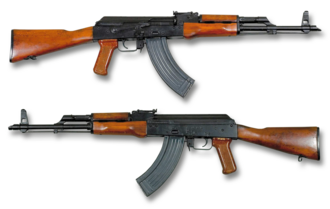
\includegraphics{../images/karabiny/akm_1.jpg}
\caption{AKM --- widok z obu stron}
\end{figure}

\begin{center}\rule{0.5\linewidth}{0.5pt}\end{center}

\subsection{Opis}\label{opis-61}

AKM (Awtomat Kałasznikowa Modernizirowannyj --- Zmodernizowany Automat
Kałasznikowa) to radziecki karabin szturmowy wprowadzony do służby w
1959 roku jako zmodernizowana wersja AK-47. Główne zmiany to redukcja
masy o \textasciitilde1 kg przez zastosowanie tłoczonego blachownicy
zamiast frezowanej, nowy kompensator skokowy na lufie oraz nowe łoże i
chwyt pistoletowy. AKM strzelający nabojem 7,62×39 mm jest jednym z
najszerzej rozpowszechnionych karabinów szturmowych w historii ---
szacuje się, że wyprodukowano ponad 50 milionów egzemplarzy różnych
klonów. Choć rosyjska armia przeszła na AK-74 (5,45 mm) w latach 70.,
AKM wciąż jest w powszechnym użyciu w siłach bezpieczeństwa, magazynach
rezerwowych i rękach aktorów niepaństwowych na całym świecie.

\subsection{Dane techniczne}\label{dane-techniczne-61}

\begin{longtable}[]{@{}ll@{}}
\toprule\noalign{}
Parametr & Wartość \\
\midrule\noalign{}
\endhead
\bottomrule\noalign{}
\endlastfoot
Typ & Karabin szturmowy \\
Kraj produkcji & ZSRR / Rosja \\
Rok wprowadzenia & 1959 \\
Kaliber & 7,62×39 mm \\
Długość & 880 mm \\
Długość lufy & 415 mm \\
Masa (bez magazynka) & 3,3 kg \\
Pojemność magazynka & 30 nabojów \\
Szybkostrzelność & 600 strz./min \\
Prędkość wylotowa & 715 m/s \\
Skuteczny zasięg & 300 m (cel punktowy) \\
\end{longtable}

\subsection{Charakterystyczne cechy
rozpoznawcze}\label{charakterystyczne-cechy-rozpoznawcze-61}

\begin{quote}
Jak odróżnić AKM od AK-74 i innych Kałasznikowów:
\end{quote}

\begin{itemize}
\tightlist
\item
  \textbf{Charakterystyczny skośny kompensator wylotowy:} AKM ma
  unikalny skośnie ścięty kompensator na końcu lufy (ścięcie pod kątem
  \textasciitilde45°) --- żaden inny AK nie ma identycznego; AK-74 ma
  cylindryczny hamulec z bocznym oknem
\item
  \textbf{Czarny lub drewniany kolba i łoże w kolorze drewna:}
  standardowy AKM ma drewniane elementy (kolba, łoże, chwyt) w kolorze
  naturalnego drewna lub ciemnobrązowym lakierze; AK-74 często ma
  brązowy lub czarny plastik
\item
  \textbf{Grubsza lufa niż AK-74:} kaliber 7,62 mm daje wyraźnie grubszą
  lufę niż AK-74 (5,45 mm) --- widoczne przy bezpośrednim porównaniu lub
  na zdjęciach z bliska
\item
  \textbf{Stalowy lub brązowy magazynek z delikatnym wygięciem:}
  magazynek AKM jest metalowy (stalowy) lub brązowy bakelit z lekkim
  wygięciem; magazynki AK-74 są wyraźnie bardziej ``bananowe'' (bardziej
  wygięte) i pomarańczowo-brązowe
\item
  \textbf{Blachownica tłoczona z widocznymi wytłoczeniami:} pudło
  zamkowe AKM ma charakterystyczne owalne wytłoczenia po obu stronach
  (wzmocnienia ścian) --- AK-47 miał pudło frezowane (grubsze, bez
  wytłoczeń)
\item
  \textbf{Tylna podstawa muszki bez bocznych skrzydełek (AKM):} muszka
  AKM jest prostsza niż w AK-74M, który ma charakterystyczne boczne
  skrzydełka ochronne
\end{itemize}

\subsection{Ciekawostka}\label{ciekawostka-61}

\begin{quote}
AKM jest prawdopodobnie bronią, która zabiła więcej ludzi niż
jakikolwiek inny wynalazek w historii ludzkości po bombie atomowej.
Michaiłowi Kałasznikowowi pytano go o to wielokrotnie --- do końca życia
twierdził, że winni są politycy, którzy dostarczali broń do konfliktów,
nie konstruktor. Przed śmiercią w 2013 roku napisał list do patriarchy
rosyjskiego Kościoła Prawosławnego z pytaniem, czy ponosi moralną
odpowiedzialność za śmierć zadaną jego bronią.
\end{quote}

\section{Karabin szturmowy AK-12}\label{karabin-szturmowy-ak-12}

\subsubsection{AK-12 Assault Rifle \textbar{}
АК-12}\label{ak-12-assault-rifle-ux430ux43a-12}

\begin{figure}
\centering
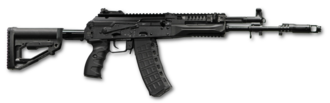
\includegraphics{../images/karabiny/ak-12_1.jpg}
\caption{AK-12 --- piąta generacja rodziny Kałasznikowa}
\end{figure}

\begin{center}\rule{0.5\linewidth}{0.5pt}\end{center}

\subsection{Opis}\label{opis-62}

AK-12 to rosyjski karabin szturmowy piątej generacji rodziny
Kałasznikowa, oficjalnie przyjęty na uzbrojenie armii rosyjskiej w
styczniu 2018 roku w ramach programu wyposażenia ``Ratnik''. Opracowany
przez Konsorcjum Kałasznikowa jako następca AK-74M, wprowadza nowoczesną
ergonomię: składaną regulowaną kolbę, pełną szynę Picatinny 1913 na
górze i po bokach, ambidekstralne sterowanie, wolnopływającą lufę dla
lepszej celności oraz nowy mechanizm spustowy z możliwością strzelania
seriami po 2 naboje z przyspieszoną cyklicznością. AK-12 jest
standardowym karabinem rosyjskiej piechoty w wojnie w Ukrainie od 2022
roku.

\subsection{Dane techniczne}\label{dane-techniczne-62}

\begin{longtable}[]{@{}ll@{}}
\toprule\noalign{}
Parametr & Wartość \\
\midrule\noalign{}
\endhead
\bottomrule\noalign{}
\endlastfoot
Typ & Karabin szturmowy \\
Kraj produkcji & Rosja \\
Rok wprowadzenia & 2018 \\
Kaliber & 5,45×39 mm \\
Długość (kolba rozłożona) & 922 mm \\
Długość (kolba złożona) & 688 mm \\
Masa (bez magazynka) & 3,5 kg \\
Pojemność magazynka & 30 nabojów \\
Szybkostrzelność & 700 strz./min \\
Prędkość wylotowa & 880--900 m/s \\
Skuteczny zasięg & 440 m \\
\end{longtable}

\subsection{Charakterystyczne cechy
rozpoznawcze}\label{charakterystyczne-cechy-rozpoznawcze-62}

\begin{quote}
Jak odróżnić AK-12 od AK-74 i AK-74M:
\end{quote}

\begin{itemize}
\tightlist
\item
  \textbf{Pełna szyna Picatinny na górnej powierzchni:} na całej górnej
  powierzchni komory zamkowej i przedniej części łoża biegnie szyna 1913
  --- w AK-74M jest tylko krótki adapter; to natychmiastowy wyróżnik
  AK-12
\item
  \textbf{Regulowana teleskopowa kolba po lewej stronie:} kolba AK-12
  składa się w lewo i jest teleskopowo regulowana (4 pozycje) --- AK-74M
  miał stałą plastikową kolbę lub boczną stałą kolbę; AK-12 wygląda
  ``nowocześniej''
\item
  \textbf{Czarna nowoczesna synthetyczna obudowa:} całkowicie czarny
  polimer na kolbie, łożu i chwycie --- wyraźnie bardziej nowoczesny
  wygląd niż drewno/bakelit starszych AK
\item
  \textbf{Ambidekstralne sterowanie bezpiecznikiem i zatrzymaniem
  zamka:} nowe przyciski i dźwignie po obu stronach komory zamkowej ---
  AK-74 miał sterowanie tylko po prawej stronie
\item
  \textbf{Wolnopływająca lufa i krótszy hamulec wylotowy:} hamulec
  wylotowy AK-12 jest krótszy i inaczej ukształtowany niż cylindryczny
  kompensator AK-74; lufa jest odizolowana od łoża
\item
  \textbf{Szyny boczne na chwycie czołowym:} boczne szyny Picatinny na
  chwycie czołowym pozwalają mocować latarki i celowniki boczne ---
  charakterystyczny element AK-12, nieobecny w AK-74
\end{itemize}

\subsection{Ciekawostka}\label{ciekawostka-62}

\begin{quote}
AK-12 przeszedł jedną z najdłuższych procedur testowania i odrzucania w
historii rosyjskiego uzbrojenia --- między 2011 a 2018 rokiem wojsko
trzykrotnie odrzucało kolejne wersje prototypowe, żądając poprawek.
Ironią historii jest, że finalnie przyjęta wersja jest tak bardzo
zmodyfikowana w stosunku do oryginalnego prototypu, że konstruktorzy
Konsorcjum Kałasznikowa żartowali, iż ``nowy AK-12 to tak naprawdę
AK-74M z plastikowym kamuflażem i szyną''.
\end{quote}

\section{Karabin szturmowy AK-103}\label{karabin-szturmowy-ak-103}

\subsubsection{AK-103 Assault Rifle \textbar{}
АК-103}\label{ak-103-assault-rifle-ux430ux43a-103}

\begin{center}\rule{0.5\linewidth}{0.5pt}\end{center}

\begin{figure}
\centering
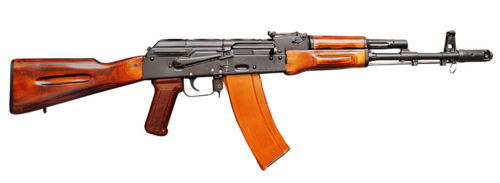
\includegraphics{../images/karabiny/ak-103_1.jpg}
\caption{AK-103 --- karabin szturmowy 7,62 mm}
\end{figure}

\subsection{Opis}\label{opis-63}

AK-103 to rosyjski karabin szturmowy kalibru 7,62×39 mm opracowany przez
Konsorcjum Kałasznikowa w 1994 roku jako wersja eksportowa z powrotem na
klasyczny nabój 7,62 mm. Jest rozwinięciem AK-74M z modernizacją
ergonomiczną, ale z powrotem wykorzystuje nabój AKM --- co czyni go
atrakcyjnym dla krajów, które mają zapasy amunicji 7,62×39 mm. AK-103 ma
czarny plastikowy chwyt, kolbę i łoże z AK-74M, ale magazynek i lufę z
AKM. Wyposażony jest w szynę boczną montażową do celowników
noktowizyjnych. Stosowany m.in. przez siły zbrojne Wenezueli, Algierii i
innych krajów arabskich, a w ostatnich latach coraz częściej przez
żołnierzy rosyjskich jako alternatywa dla AK-12 (ze względu na większą
energię naboju 7,62 mm).

\subsection{Dane techniczne}\label{dane-techniczne-63}

\begin{longtable}[]{@{}ll@{}}
\toprule\noalign{}
Parametr & Wartość \\
\midrule\noalign{}
\endhead
\bottomrule\noalign{}
\endlastfoot
Typ & Karabin szturmowy \\
Kraj produkcji & Rosja \\
Rok wprowadzenia & 1994 \\
Kaliber & 7,62×39 mm \\
Długość (kolba rozłożona) & 943 mm \\
Długość (kolba złożona) & 704 mm \\
Długość lufy & 415 mm \\
Masa (bez magazynka) & 3,4 kg \\
Pojemność magazynka & 30 nabojów \\
Prędkość wylotowa & 715 m/s \\
Skuteczny zasięg & 400 m \\
\end{longtable}

\subsection{Charakterystyczne cechy
rozpoznawcze}\label{charakterystyczne-cechy-rozpoznawcze-63}

\begin{quote}
Jak odróżnić AK-103 od AK-74M i AKM:
\end{quote}

\begin{itemize}
\tightlist
\item
  \textbf{Czarny plastikowy chwyt i łoże --- jak AK-74M, ale nabój
  7,62:} z zewnątrz AK-103 wygląda jak AK-74M (czarny plastik), ale ma
  wyraźnie grubszy magazynek kalibru 7,62 mm --- to kluczowy
  identyfikator
\item
  \textbf{Grubszy magazynek z lekkim wygięciem 7,62 mm:} magazynek
  AK-103 (7,62×39) jest grubszy i bardziej wygięty niż smukły
  pomarańczowy AK-74; bardziej podobny do magazynka AKM, ale czarny
\item
  \textbf{Hamulec wylotowy taki sam jak AK-74M:} na końcu lufy AK-103
  widnieje charakterystyczny cylindryczny hamulec wylotowy identyczny
  jak w AK-74M --- to odróżnia go od AKM (skośny kompensator)
\item
  \textbf{Boczna szyna montażowa po lewej:} charakterystyczna metalowa
  szyna z boku komory zamkowej (po lewej) do mocowania celowników
  noktowizyjnych --- obecna w AK-103, nie ma jej w starszym AKM
\item
  \textbf{Czarna plastikowa składana kolba (bok lewy):} kolba AK-103
  jest czarnym plastikiem, składa się na lewo --- podobnie jak AK-74M;
  stary AKM miał drewnianą lub stałą plastikową kolbę
\item
  \textbf{Grubsza lufa niż AK-74:} kaliber 7,62 mm daje wyraźnie grubszą
  lufę niż AK-74/AK-103 --- przy bezpośrednim porównaniu różnica 5,45 vs
  7,62 mm jest widoczna
\end{itemize}

\subsection{Ciekawostka}\label{ciekawostka-63}

\begin{quote}
AK-103 był pierwszym karabinem Kałasznikowa oficjalnie zaoferowanym w
wersji z tłumikiem dźwięku w katalogu eksportowym Konsorcjum
Kałasznikowa --- co było przełomem, bo wcześniej sowiecka doktryna
negowała potrzebę tłumienia broni indywidualnej. Wenezuela zamówiła
fabrykę licencyjną produkującą AK-103 i rozdała je milicjom obywatelskim
--- co sprawiło, że w 2019 roku zachodnie media alarmowały o
``uzbrojeniu Ameryki Łacińskiej w Kałasznikowy''.
\end{quote}

\section{Karabin szturmowy AK-15}\label{karabin-szturmowy-ak-15}

\subsubsection{AK-15 Assault Rifle \textbar{}
АК-15}\label{ak-15-assault-rifle-ux430ux43a-15}

\begin{center}\rule{0.5\linewidth}{0.5pt}\end{center}

\begin{figure}
\centering
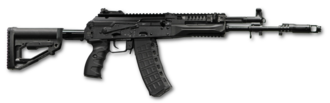
\includegraphics{../images/karabiny/ak-15_1.jpg}
\caption{AK-15 --- karabin szturmowy nowej generacji}
\end{figure}

\subsection{Opis}\label{opis-64}

AK-15 to rosyjski karabin szturmowy kalibru 7,62×39 mm opracowany przez
Konsorcjum Kałasznikowa w 2016 roku jako wersja AK-12 przywracająca
klasyczny nabój 7,62 mm. Jest bezpośrednim odpowiednikiem AK-12 ---
dzieli z nim niemal identyczną platformę (kolba, chwyt, interfejs) ---
ale używa cięższego naboju o większej energii, atrakcyjnego dla
żołnierzy wymagających lepszego rażenia. AK-15 został przyjęty na
uzbrojenie armii rosyjskiej w 2018 roku równocześnie z AK-12, jako
alternatywa dla oddziałów preferujących kaliber 7,62 mm. W
przeciwieństwie do AK-103 (który jest modernizacją linii AK-74M), AK-15
jest zbudowany od podstaw na nowoczesnej platformie nowej generacji z
magistralą Picatinny i ergonomią XXI wieku.

\subsection{Dane techniczne}\label{dane-techniczne-64}

\begin{longtable}[]{@{}ll@{}}
\toprule\noalign{}
Parametr & Wartość \\
\midrule\noalign{}
\endhead
\bottomrule\noalign{}
\endlastfoot
Typ & Karabin szturmowy \\
Kraj produkcji & Rosja \\
Rok wprowadzenia & 2018 \\
Kaliber & 7,62×39 mm \\
Długość (kolba rozłożona) & 940 mm \\
Długość (kolba złożona) & 690 mm \\
Długość lufy & 415 mm \\
Masa (bez magazynka) & 3,8 kg \\
Pojemność magazynka & 30 nabojów \\
Prędkość wylotowa & 730 m/s \\
Skuteczny zasięg & 400 m \\
\end{longtable}

\subsection{Charakterystyczne cechy
rozpoznawcze}\label{charakterystyczne-cechy-rozpoznawcze-64}

\begin{quote}
Jak odróżnić AK-15 od AK-12 i AK-103:
\end{quote}

\begin{itemize}
\tightlist
\item
  \textbf{Identyczna sylwetka jak AK-12 --- różnica w magazynku:} AK-15
  i AK-12 są wizualnie niemal identyczne; jedyną oczywistą różnicą jest
  grubszy, bardziej wygięty czarny magazynek kalibru 7,62 mm zamiast
  smukłego magazynka 5,45 mm w AK-12
\item
  \textbf{Grubszy magazynek 7,62 mm --- czarny, wyraźnie bardziej
  wygięty niż AK-12:} magazynek AK-15 jest zbliżony kształtem do
  magazynka AKM, ale wykonany z czarnego polimeru --- bez wygięcia
  łukowatego jak w AKM, ale grubszy niż AK-12
\item
  \textbf{Czarna kolba teleskopowa z regulacją pochylenia:} obie wersje
  (AK-12 i AK-15) mają tę samą charakterystyczną kolbę regulowaną ---
  nowość niemożliwa w AK-74M i AK-103
\item
  \textbf{Górna szyna Picatinny na całej długości nakrywki:} długa
  płaska szyna na nakrywce komory zamkowej --- cecha charakterystyczna
  nowej generacji AK; AK-103 i AK-74M mają tylko boczną szynę lub w
  ogóle jej nie mają
\item
  \textbf{Dwie szyny boczne i dolna szyna na łożu:} cztery szyny
  Picatinny (góra + 2 boki + dół) na łożu --- nowoczesny wygląd
  taktyczny; starsze AK mają gładkie drewniane lub plastikowe łoże bez
  szyn
\item
  \textbf{Hamulec wylotowy z AK-12 --- inny niż klasyczny AK:} na
  wylocie lufy AK-15 widnieje nowy prosty hamulec/tłumik płomienia ---
  inny od cylindrycznego hamulca AK-74M i skośnego AKM
\end{itemize}

\subsection{Ciekawostka}\label{ciekawostka-64}

\begin{quote}
AK-15 powstał po tym, jak część oficerów rosyjskich sił specjalnych
odmówiła przestawienia się na kaliber 5,45 mm --- argumentując, że nabój
7,62×39 mm ma lepszą zdolność penetracji ścian, samochodów i lekkich
osłon balistycznych. W rezultacie Rosjanie utrzymują dwa równoległe
standardy karabinów szturmowych: AK-12 (5,45 mm) dla piechoty i AK-15
(7,62 mm) dla specjalsów i oddziałów wymagających większej siły rażenia.
\end{quote}

\section{Karabin szturmowy AN-94
Abakan}\label{karabin-szturmowy-an-94-abakan}

\subsubsection{AN-94 Abakan Assault Rifle \textbar{} АН-94
«Абакан»}\label{an-94-abakan-assault-rifle-ux430ux43d-94-ux430ux431ux430ux43aux430ux43d}

\begin{center}\rule{0.5\linewidth}{0.5pt}\end{center}

\begin{figure}
\centering
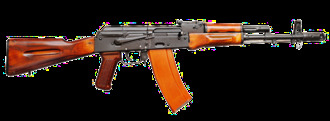
\includegraphics{../images/karabiny/an-94_1.jpg}
\caption{AN-94 Abakan --- karabin szturmowy}
\end{figure}

\subsection{Opis}\label{opis-65}

AN-94 Abakan (Авт. Никонова --- Автомат Никонова) to rosyjski karabin
szturmowy kalibru 5,45×39 mm zaprojektowany przez Gennadija Nikonowa i
przyjęty do służby w 1994 roku jako zwycięzca programu ``Abakan''
mającego zastąpić AK-74. Wyróżnia się unikatowym mechanizmem ``zwrotu
kluzy'' (shifted pulse) --- pierwsze dwa naboje oddawane są w seriach
dwustrzałowych z tempem 1800 strz./min, zanim odrzut dosięgnie strzelca.
Dzięki temu celność krótkich serii jest znacznie lepsza niż AK-74.
Mechanizm jest jednak bardzo złożony i kosztowny --- co spowodowało, że
AN-94 nigdy nie zastąpił masowo AK-74, lecz służy głównie w oddziałach
specjalnych i elitarnych jednostkach armii rosyjskiej.

\subsection{Dane techniczne}\label{dane-techniczne-65}

\begin{longtable}[]{@{}
  >{\raggedright\arraybackslash}p{(\columnwidth - 2\tabcolsep) * \real{0.5263}}
  >{\raggedright\arraybackslash}p{(\columnwidth - 2\tabcolsep) * \real{0.4737}}@{}}
\toprule\noalign{}
\begin{minipage}[b]{\linewidth}\raggedright
Parametr
\end{minipage} & \begin{minipage}[b]{\linewidth}\raggedright
Wartość
\end{minipage} \\
\midrule\noalign{}
\endhead
\bottomrule\noalign{}
\endlastfoot
Typ & Karabin szturmowy z mechanizmem kompensacji odrzutu \\
Kraj produkcji & Rosja \\
Rok wprowadzenia & 1994 \\
Kaliber & 5,45×39 mm \\
Długość (kolba rozłożona) & 943 mm \\
Długość (kolba złożona) & 728 mm \\
Długość lufy & 405 mm \\
Masa (bez magazynka) & 3,85 kg \\
Pojemność magazynka & 30 lub 60 nabojów \\
Szybkostrzelność & 600 strz./min (normalnie) / 1800 strz./min (serie
2-strz.) \\
Skuteczny zasięg & 500 m \\
\end{longtable}

\subsection{Charakterystyczne cechy
rozpoznawcze}\label{charakterystyczne-cechy-rozpoznawcze-65}

\begin{quote}
Jak odróżnić AN-94 od AK-74 i AK-12:
\end{quote}

\begin{itemize}
\tightlist
\item
  \textbf{Charakterystyczne przesunięte (skośne) łoże i komora zamkowa:}
  AN-94 nie wygląda jak klasyczny AK --- lufa i mechanizm strzelający są
  przesunięte względem kolby pod kątem, co daje całej broni
  charakterystyczny ``pochylony'' wygląd
\item
  \textbf{Chwyt pistoletowy daleko z przodu i nisko:} AN-94 ma chwyt
  pistoletowy wyraźnie wyżej i bardziej z przodu niż AK-74 --- zupełnie
  inny profil trzymania
\item
  \textbf{Brak zewnętrznego gazownika nad lufą (jest wewnątrz):} w
  odróżnieniu od AK-74, AN-94 nie ma wyraźnego bloku gazownika z muszką
  na lufie --- układ gazowy jest ukryty, a muszka stoi na czubku lufy
  bez podstawy gazowej
\item
  \textbf{Składana plastikowa kolba po prawej stronie:} kolba AN-94
  składa się na prawą stronę --- odwrotnie niż AK-74M (lewa strona) ---
  i jest w charakterystycznym ciemnoszarym odcieniu
\item
  \textbf{Podwójny magazynek 60-nabojowy lub standardowy 30-nabojowy:}
  AN-94 może używać specjalnego dwukomorowego magazynka 60-nabojowego
  (dwie komory połączone) --- bardzo rzadki widok przy karabinach
  szturmowych
\item
  \textbf{Całkowicie odmienna sylwetka od klasycznego AK:} AN-94 wygląda
  jak odrębna rodzina broni, nie jak AK --- kto zna AK-74, natychmiast
  zobaczy, że AN-94 to coś innego
\end{itemize}

\subsection{Ciekawostka}\label{ciekawostka-65}

\begin{quote}
AN-94 wygrał program ``Abakan'' pokonując 12 konkurentów, w tym AEK-971.
Jednak armia rosyjska nigdy nie zamawiała go masowo --- między innymi
dlatego, że AN-94 jest 6 razy droższy w produkcji niż AK-74 i wymaga
specjalistycznego szkolenia. Karabin jest tak mechanicznie złożony, że
serwis polowy jest praktycznie niemożliwy bez warsztatowych narzędzi.
Żołnierze narzekali, że ``działa wspaniale, gdy jest czysty --- ale w
błocie i piasku przestaje działać wcześniej niż AK''. Mimo to AN-94
pojawia się regularnie w oficjalnych pokazach wojskowych i jest symbolem
rosyjskiej myśli technicznej lat 90.
\end{quote}

\section{Karabin szturmowy AEK-971}\label{karabin-szturmowy-aek-971}

\subsubsection{AEK-971 Assault Rifle \textbar{}
АЕК-971}\label{aek-971-assault-rifle-ux430ux435ux43a-971}

\begin{center}\rule{0.5\linewidth}{0.5pt}\end{center}

\begin{figure}
\centering
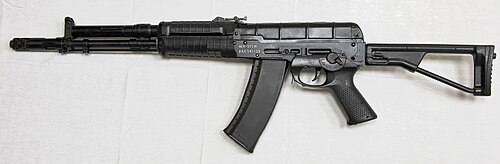
\includegraphics{../images/karabiny/aek-971_1.jpg}
\caption{AEK-971 --- karabin szturmowy ze zrównoważoną automatyką}
\end{figure}

\subsection{Opis}\label{opis-66}

AEK-971 to rosyjski karabin szturmowy kalibru 5,45×39 mm (wersja AEK-973
to 7,62×39 mm) zaprojektowany w Kowrowie przez Stanisława Koksharova i
Borysa Garyova. Wyróżnia się mechanizmem zrównoważonej automatyki
(zbilansowanej automatyki) --- dodatkowa masa poruszająca się w
przeciwną stronę niż zamek niweluje odrzut, drastycznie zmniejszając
podrzut lufy przy seriach. W programie ``Abakan'' AEK-971 przegrał z
AN-94, ale w 2015 roku wrócił na rynek jako podstawa rodziny A-545 i
A-762 --- przyjętych na uzbrojenie wojsk rosyjskich w 2018 roku jako
uzupełnienie AK-12 i AK-15. A-545/A-762 (nowsze wersje AEK-971) są
stosowane przez rosyjskie siły specjalne i oddziały Gwardii Narodowej
(Rosgwardia).

\subsection{Dane techniczne}\label{dane-techniczne-66}

\begin{longtable}[]{@{}ll@{}}
\toprule\noalign{}
Parametr & Wartość \\
\midrule\noalign{}
\endhead
\bottomrule\noalign{}
\endlastfoot
Typ & Karabin szturmowy ze zrównoważoną automatyką \\
Kraj produkcji & Rosja \\
Rok wprowadzenia & A-545/A-762: 2018 (prototyp AEK-971: lata 80.) \\
Kaliber & 5,45×39 mm (A-545) / 7,62×39 mm (A-762) \\
Długość (kolba rozłożona) & 960 mm \\
Długość (kolba złożona) & 725 mm \\
Długość lufy & 415 mm \\
Masa (bez magazynka) & 3,5 kg \\
Pojemność magazynka & 30 nabojów \\
Szybkostrzelność & 850 strz./min \\
Skuteczny zasięg & 500 m \\
\end{longtable}

\subsection{Charakterystyczne cechy
rozpoznawcze}\label{charakterystyczne-cechy-rozpoznawcze-66}

\begin{quote}
Jak odróżnić AEK-971/A-545 od AK-12 i AN-94:
\end{quote}

\begin{itemize}
\tightlist
\item
  \textbf{Charakterystyczny port wentylacyjny na górze komory zamkowej:}
  AEK-971/A-545 ma wyraźny otwór lub szczelinę wentylacyjną na górze
  tylnej części komory zamkowej --- widoczny element związany z
  mechanizmem zrównoważonej automatyki; AK-12 go nie ma
\item
  \textbf{Prosty, klasyczny układ podobny do AK --- ale chwyt cofnięty:}
  sylwetka AEK-971 przypomina AK, ale chwyt pistoletowy jest cofnięty
  dalej ku tyłowi niż w standardowym AK --- daje to charakterystyczną
  bryłę
\item
  \textbf{Kolba rurowa lub teleskopowa --- inna geometria niż AK-74M:}
  AEK-971 miał charakterystyczną metalową kolbę rurową; A-545 ma
  nowocześniejszą regulowaną kolbę polimeru podobną do AK-12
\item
  \textbf{Hamulec wylotowy w kształcie ``klatki'' (cage-style):} A-545
  wyposażony jest w charakterystyczny kompensator/hamulec w formie
  cylindrycznej klatki --- inny niż hamulec AK-12 i AK-15
\item
  \textbf{Brak zewnętrznej różnicy wizualnej między A-545 a A-762:}
  wersje 5,45 mm i 7,62 mm A-545/A-762 wyglądają identycznie --- różnica
  tylko w magazynku (smukły 5,45 vs grubszy 7,62)
\item
  \textbf{Szyny Picatinny w układzie zbliżonym do AK-12:} cztery szyny
  taktyczne jak w AK-12 --- góra/boki/dół; sprawia, że A-545 można
  pomylić z AK-12 bez bliskiego oglądania
\end{itemize}

\subsection{Ciekawostka}\label{ciekawostka-66}

\begin{quote}
AEK-971 przegrał konkurs ``Abakan'' z AN-94 na początku lat 90., ale
miał niezwykłą drugą szansę --- gdy armia rosyjska, niezadowolona z
wysokiej ceny AN-94, ogłosiła w 2011 roku konkurs na ``Ratnik''
(żołnierz przyszłości). AEK-971 w unowocześnionej formie (A-545) pokonał
tym razem AK-12 w testach celności przy ogniu automatycznym ---
uzyskując wyraźnie lepsze skupienie. Mimo to wojsko zdecydowało się
przyjąć oba: AK-12/AK-15 (tańsze, dla masowej piechoty) i A-545/A-762
(droższe, ale celniejsze, dla specjalsów). To rzadki przypadek, gdy
armia kupiła i wygrany, i przegrany projekt naraz.
\end{quote}

\section{Karabin szturmowy SR-3 Wihr}\label{karabin-szturmowy-sr-3-wihr}

\subsubsection{SR-3 Vikhr Assault Rifle \textbar{} СР-3
«Вихрь»}\label{sr-3-vikhr-assault-rifle-ux441ux440-3-ux432ux438ux445ux440ux44c}

\begin{center}\rule{0.5\linewidth}{0.5pt}\end{center}

\begin{figure}
\centering
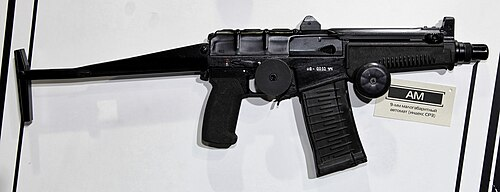
\includegraphics{../images/karabiny/sr-3_1.jpg}
\caption{SR-3 Wihr --- kompaktowy karabin szturmowy}
\end{figure}

\subsection{Opis}\label{opis-67}

SR-3 Wihr (Вихрь --- Wicher) to rosyjski kompaktowy karabin szturmowy
kalibru 9×39 mm opracowany przez TsNIITochMash w latach 90. dla FSB, FSO
i rosyjskich służb specjalnych. Używa poddźwiękowego naboju 9×39 mm
przeznaczonego pierwotnie dla tłumionej broni specjalnej (AS Val, VSS
Wintorez) --- co pozwala na stosowanie tłumika dźwięku z bardzo dobrą
efektywnością. SR-3 jest kompaktowy (nieco dłuższy od pistoletu
maszynowego), wysoce manewrowy w pomieszczeniach i zdolny do penetracji
lekkich kamizelek balistycznych na odległość do 200 m. To broń wybitnie
specjalna --- w odróżnieniu od karabinów szturmowych ogólnego
przeznaczenia; stosowana głównie przez antyterrorystów, ochronę VIP i
miejskie oddziały specjalne.

\subsection{Dane techniczne}\label{dane-techniczne-67}

\begin{longtable}[]{@{}ll@{}}
\toprule\noalign{}
Parametr & Wartość \\
\midrule\noalign{}
\endhead
\bottomrule\noalign{}
\endlastfoot
Typ & Kompaktowy karabin szturmowy / PDW \\
Kraj produkcji & Rosja \\
Rok wprowadzenia & 1996 \\
Kaliber & 9×39 mm \\
Długość (kolba rozłożona) & 610 mm \\
Długość (kolba złożona) & 360 mm \\
Długość lufy & 172 mm \\
Masa (bez magazynka) & 2,0 kg \\
Pojemność magazynka & 20 lub 30 nabojów \\
Prędkość wylotowa & 295 m/s (poddźwiękowa) \\
Skuteczny zasięg & 200 m \\
\end{longtable}

\subsection{Charakterystyczne cechy
rozpoznawcze}\label{charakterystyczne-cechy-rozpoznawcze-67}

\begin{quote}
Jak odróżnić SR-3 od AKS-74U i AS Val:
\end{quote}

\begin{itemize}
\tightlist
\item
  \textbf{Bardzo mała i krótka broń --- mniejsza niż AKS-74U:} SR-3 ze
  złożoną kolbą ma zaledwie 360 mm --- to rozmiar dużego pistoletu;
  AKS-74U ma 490 mm; SR-3 jest tak mała, że często trudno ją
  zidentyfikować jako karabin szturmowy
\item
  \textbf{Brak zewnętrznego tłumika (ale możliwość montażu):}
  standardowy SR-3 nie ma tłumika (w odróżnieniu od AS Val i VSS) --- za
  to możliwe jest szybkie dołączenie krótkiego tłumika; ten sam nabój
  9×39 mm bez tłumika jest wyraźnie głośniejszy niż AS Val
\item
  \textbf{Metalowa kolba szkieletowa składana na prawą stronę:} kolba
  SR-3 to metalowa kratownica składana na prawo --- charakterystyczny
  wygląd, inny od plastikowej kolby AKS-74U
\item
  \textbf{Krótkie, masywne łoże bez wyraźnego odcięcia:} SR-3 ma bardzo
  krótkie łoże z uchwytem przednim --- sylwetka jest ``zaokrąglona'' i
  kompaktowa, bez charakterystycznej długiej lufy AK
\item
  \textbf{Grubszy magazynek 9×39 mm --- inny niż AKS-74U:} magazynek
  SR-3 jest krótszy i grubszy niż magazynek AKS-74U (kaliber 5,45 mm)
  --- przy bezpośrednim porównaniu wyraźna różnica w wymiarach pudełka
  magazynka
\item
  \textbf{Charakterystyczny przód broni bez gazownika ponad lufą:} SR-3
  nie ma tradycyjnego bloku gazownika z muszką ponad lufą; układ jest
  uproszczony, a muszka siedzi bezpośrednio na rurze lufy
\end{itemize}

\subsection{Ciekawostka}\label{ciekawostka-67}

\begin{quote}
SR-3 Wihr ``zasłynął'' w mediach po zamachu na Dubrowce w 2002 roku
(teatr na Dubrowce, ``Nord-Ost'') --- agenci FSB szturmujący teatr byli
uzbrojeni w SR-3. Brak wyraźnych fotografii z szturmu przez lata
utrudniał identyfikację broni. Gdy w końcu zidentyfikowano SR-3 na
nagraniach, zrozumiano dlaczego: SR-3 jest tak mały, że operatorzy FSB
mogli go nosić ukryty pod ubraniem cywilnym aż do momentu szturmu --- co
byłoby niemożliwe z AKS-74U.
\end{quote}

\section{Karabin szturmowy AS Val}\label{karabin-szturmowy-as-val}

\subsubsection{AS Val Assault Rifle \textbar{} АС
«Вал»}\label{as-val-assault-rifle-ux430ux441-ux432ux430ux43b}

\begin{center}\rule{0.5\linewidth}{0.5pt}\end{center}

\begin{figure}
\centering
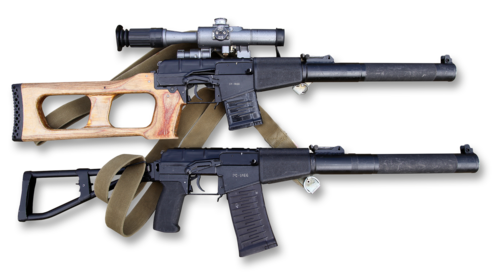
\includegraphics{../images/karabiny/as-val_1.jpg}
\caption{AS Val --- tłumiony karabin szturmowy}
\end{figure}

\subsection{Opis}\label{opis-68}

AS Val (Автомат Специальный Вал --- Wał) to rosyjski tłumiony karabin
szturmowy kalibru 9×39 mm opracowany przez TsNIITochMash w 1987 roku dla
sił specjalnych i służb wywiadowczych ZSRR/Rosji. Tłumik jest integralną
częścią konstrukcji (nie demontuje się go do użytku bojowego) --- razem
z poddźwiękowym nabojem 9×39 mm daje jedną z najcichszych broni
automatycznych na świecie. AS Val i jego siostrzana broń snajperska VSS
Wintorez zostały zaprojektowane do cichego eliminowania celów w
pancerzach osobistych --- nabój 9×39 mm przebija kamizelki klasy III do
500 m. Broń służy głównie w FSB, FSO, GRU i Spetsnaz; pojawiła się w
Czeczenii, Afganistanie i na Ukrainie.

\subsection{Dane techniczne}\label{dane-techniczne-68}

\begin{longtable}[]{@{}ll@{}}
\toprule\noalign{}
Parametr & Wartość \\
\midrule\noalign{}
\endhead
\bottomrule\noalign{}
\endlastfoot
Typ & Tłumiony karabin szturmowy \\
Kraj produkcji & Rosja \\
Rok wprowadzenia & 1987 \\
Kaliber & 9×39 mm \\
Długość & 875 mm (tłumik zintegrowany, stały) \\
Długość lufy & 200 mm \\
Masa (z tłumikiem) & 2,96 kg \\
Pojemność magazynka & 20 nabojów \\
Prędkość wylotowa & 290--295 m/s (poddźwiękowa) \\
Skuteczny zasięg & 300--400 m (z optiką) \\
\end{longtable}

\subsection{Charakterystyczne cechy
rozpoznawcze}\label{charakterystyczne-cechy-rozpoznawcze-68}

\begin{quote}
Jak odróżnić AS Val od VSS Wintorez i SR-3:
\end{quote}

\begin{itemize}
\tightlist
\item
  \textbf{Duży integrowany tłumik na całą długość lufy --- nie do
  zdjęcia:} tłumik AS Val jest trwale wbudowany w broń i stanowi jej
  przód --- broń wygląda jakby miała bardzo grubą, długą ``lufę''; żaden
  inny masowo stosowany karabin szturmowy nie ma stałego tłumika
\item
  \textbf{Brak kolby składanej standardowej --- kolba drewniana lub
  metalowa szkieletowa:} AS Val często jest wyposażony w drewnianą kolbę
  wyglądającą archaicznie --- bo pochodzi z czasów sowieckich; nowsze
  wersje mają metalową kolbę składaną, ale nadal wyróżniają się sylwetką
\item
  \textbf{Tłumik wyraźnie grubszy niż lufa --- cylindryczny:} tłumik
  zintegrowany AS Val ma charakterystyczny cylindryczny kształt o
  średnicy znacznie większej niż lufa; od strony czołowej broń wygląda
  jak gruba rura
\item
  \textbf{Różnica wobec VSS Wintorez --- brak gniazda optyki i inny
  chwyt:} VSS ma standardowe gniazdo celownika optycznego na górze i
  smuklejszy kształt; AS Val jest przeznaczony bardziej do ognia
  automatycznego --- ma większy magazynek (20 zamiast 10) i brak
  standardowej szyny optycznej w starszych wersjach
\item
  \textbf{Grubszy magazynek 9×39 mm --- porównywalny z SR-3:} magazynek
  AS Val jest krótki i gruby (kaliber 9 mm) --- wyraźnie inny od
  smukłych magazynków 5,45 mm AK-74 i AKS-74U
\item
  \textbf{Bardzo charakterystyczna ``głucha'' sylwetka z przodu:} z
  profilu AS Val ma zupełnie inny wygląd niż AK --- brak wyraźnego
  otworu wylotowego lufy (tłumik go zasłania), brak muszki na końcu,
  brak hamulca wylotowego
\end{itemize}

\subsection{Ciekawostka}\label{ciekawostka-68}

\begin{quote}
AS Val i VSS Wintorez były przez wiele lat bronią objętą ścisłą
tajemnicą --- formalnie nie istniały w sowieckich/rosyjskich katalogach
wojskowych. Pierwszy raz potwierdzono ich istnienie dopiero w 1994 roku,
gdy Rosja wystawiła je na targach IDEX w Abu Zabi. Do dziś szczegóły
techniczne niektórych wersji amunicji 9×39 mm używanej przez rosyjskie
służby specjalne są klasyfikowane. Broń zyskała zainteresowanie
zachodnie po jej zdobyciu na polach bitew Czeczenii i Syrii --- i do
dziś uchodzi za jeden z najbardziej zaawansowanych systemów broni
osobistej na świecie.
\end{quote}

\section{Ręczny karabin maszynowy
RPK}\label{rux119czny-karabin-maszynowy-rpk}

\subsubsection{RPK Light Machine Gun \textbar{} РПК (Ручной пулемёт
Калашникова)}\label{rpk-light-machine-gun-ux440ux43fux43a-ux440ux443ux447ux43dux43eux439-ux43fux443ux43bux435ux43cux451ux442-ux43aux430ux43bux430ux448ux43dux438ux43aux43eux432ux430}

\begin{center}\rule{0.5\linewidth}{0.5pt}\end{center}

\begin{figure}
\centering
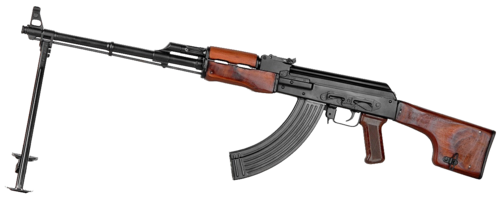
\includegraphics{../images/karabiny_maszynowe/rpk_1.jpg}
\caption{RPK --- ręczny karabin maszynowy}
\end{figure}

\subsection{Opis}\label{opis-69}

RPK (Ручной пулемёт Калашникова --- Ręczny karabin maszynowy
Kałasznikowa) to radziecka lekka broń wsparcia kalibru 7,62×39 mm
opracowana przez Michaiła Kałasznikowa i przyjęta do służby w 1961 roku.
Stanowi wersję wsparcia ogniowego AKM --- ma tę samą mechanikę i
wymienną amunicję, ale cięższy lufy, stałą kolbę drewnianą i dwójnóg, co
poprawia celność przy ogniu ciągłym. RPK używa standardowych magazynków
AKM (30 nabojów) lub specjalnych bębnowych magazynków 40- i
75-nabojowych. Zasięg skuteczny do 800 m. W drugiej połowie lat 70.
zastąpiony przez RPK-74 (kaliber 5,45 mm), jednak RPK wciąż jest na
wyposażeniu wielu armii i nieregularnych sił zbrojnych.

\subsection{Dane techniczne}\label{dane-techniczne-69}

\begin{longtable}[]{@{}ll@{}}
\toprule\noalign{}
Parametr & Wartość \\
\midrule\noalign{}
\endhead
\bottomrule\noalign{}
\endlastfoot
Typ & Ręczny karabin maszynowy (LMG) \\
Kraj produkcji & ZSRR / Rosja \\
Rok wprowadzenia & 1961 \\
Kaliber & 7,62×39 mm \\
Długość & 1 040 mm \\
Długość lufy & 590 mm \\
Masa (bez magazynka) & 4,8 kg \\
Pojemność magazynka & 40 lub 75 nabojów (bębnowy) \\
Szybkostrzelność & 600 strz./min \\
Skuteczny zasięg & 800 m \\
\end{longtable}

\subsection{Charakterystyczne cechy
rozpoznawcze}\label{charakterystyczne-cechy-rozpoznawcze-69}

\begin{quote}
Jak odróżnić RPK od AKM i PKM:
\end{quote}

\begin{itemize}
\tightlist
\item
  \textbf{Wyraźnie dłuższa lufa niż AKM --- ok. 59 cm zamiast 41 cm:}
  RPK jest wyraźnie dłuższy od AKM; przy porównaniu obu broni lufa RPK
  wystaje daleko poza łoże; ta długość jest pierwszym i najważniejszym
  identyfikatorem
\item
  \textbf{Dwójnóg pod lufą --- składany w przód:} RPK ma
  charakterystyczny dwójnóg (bipod) tuż przy wylocie lufy; w pozycji
  złożonej leży wzdłuż lufy; żaden standardowy AKM nie ma dwójnogu
\item
  \textbf{Stała drewniana lub plastikowa kolba bez możliwości
  składania:} RPK ma stałą kolbę (nie składaną jak AKS lub RPKS); kolba
  jest szersza i stabilniejsza od kolby AKM --- różnica widoczna przy
  porównaniu kształtu tylca
\item
  \textbf{Szerszy trzon kolby i płetwowata stopka:} stopka kolby RPK
  jest szersza i ma charakterystyczny kształt trapezoidalny --- lepsza
  stabilizacja w czasie ognia ciągłego; AKM ma węższy, prostszy tylec
\item
  \textbf{Bębnowy magazynek 75-nabojowy --- wyróżniający cechą:} jeśli
  RPK jest załadowany bębnem 75-nabojowym, wygląda zupełnie inaczej niż
  AKM --- wielki okrągły magazynek pod bronią jest nie do pomylenia
\item
  \textbf{Wyraźnie lżejszy i krótszy od PKM:} PKM jest ciężkim karabinem
  maszynowym na trójnogu lub dwójnogu, z taśmą --- RPK jest wyraźnie
  mniejszy, kompaktowszy i zasilany z magazynka, nie taśmy
\end{itemize}

\subsection{Ciekawostka}\label{ciekawostka-69}

\begin{quote}
RPK trafił do Wietnamu Północnego przed RPK-74 --- i stał się
najczęściej stosowaną bronią wsparcia piechoty Viet Congu. Żołnierze
amerykańscy opisywali go jako ``AK z długą lufą'' i przez długi czas
mylnie identyfikowali na zdjęciach jako RPD lub DP. Ciekawostką jest, że
Vietnamese People's Army (armia Wietnamu Północnego) preferowała RPK od
chińskich odpowiedników ze względu na wspólną amunicję z AKM ---
logistycznie prościej było utrzymywać jeden kaliber dla całego oddziału.
\end{quote}

\section{Ręczny karabin maszynowy
RPL-20}\label{rux119czny-karabin-maszynowy-rpl-20}

\subsubsection{RPL-20 Light Machine Gun \textbar{}
РПЛ-20}\label{rpl-20-light-machine-gun-ux440ux43fux43b-20}

\begin{center}\rule{0.5\linewidth}{0.5pt}\end{center}

\begin{figure}
\centering
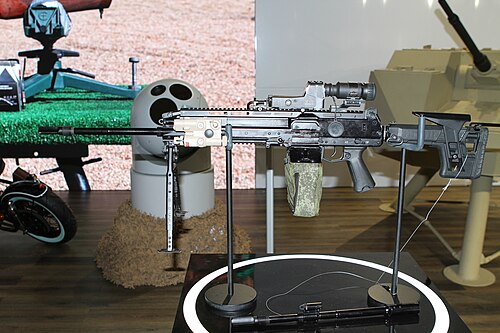
\includegraphics{../images/karabiny_maszynowe/rpl-20_1.jpg}
\caption{RPL-20 --- ręczny karabin maszynowy}
\end{figure}

\subsection{Opis}\label{opis-70}

RPL-20 to rosyjski nowoczesny ręczny karabin maszynowy kalibru 5,45×39
mm opracowany przez Konsorcjum Kałasznikowa i zaprezentowany po raz
pierwszy w 2021 roku jako broń piechoty nowej generacji w ramach
programu ``Ratnik-3''. Jest bezpośrednim następnikiem RPK-74M --- używa
tej samej amunicji i podobnej mechaniki, ale ma zupełnie nową ergonomię:
szyny Picatinny, regulowaną kolbę, nowoczesne łoże i poprawiony system
oddechowy lufy. Wyposażony w pojemnik taśmowy (kaseta 200 nabojów)
zamiast tradycyjnych magazynków, co znacznie zwiększa wydajność ognia
ciągłego. Stan służby: ograniczone przyjęcie w 2022--2023, trwa
doposażanie wybranych jednostek.

\subsection{Dane techniczne}\label{dane-techniczne-70}

\begin{longtable}[]{@{}ll@{}}
\toprule\noalign{}
Parametr & Wartość \\
\midrule\noalign{}
\endhead
\bottomrule\noalign{}
\endlastfoot
Typ & Ręczny karabin maszynowy nowej generacji \\
Kraj produkcji & Rosja \\
Rok wprowadzenia & 2022 (ograniczone) \\
Kaliber & 5,45×39 mm \\
Długość (kolba rozłożona) & 1 000 mm \\
Długość lufy & 550 mm \\
Masa (bez amunicji) & 5,5 kg \\
Pojemność & 200 nabojów (kaseta taśmowa) lub mag. 45 nab. \\
Szybkostrzelność & 700 strz./min \\
Skuteczny zasięg & 800 m \\
\end{longtable}

\subsection{Charakterystyczne cechy
rozpoznawcze}\label{charakterystyczne-cechy-rozpoznawcze-70}

\begin{quote}
Jak odróżnić RPL-20 od RPK-74M i PKP Pieczeniegu:
\end{quote}

\begin{itemize}
\tightlist
\item
  \textbf{Kaseta taśmowa 200 nabojów pod bronią --- charakterystyczny
  ``pojemnik'':} RPL-20 może być zasilany z kasety z taśmą montowanej
  pod bronią --- kwadratowy plastikowy pojemnik pod kolbą strzelca;
  żaden RPK nie ma takiego podajnika; to najważniejszy identyfikator
\item
  \textbf{Nowoczesna ergonomia: szyny Picatinny, regulowana kolba,
  uchwyt kątowy:} RPL-20 ma wygląd nowoczesnej zachodniej broni wsparcia
  --- szyny na całym obwodzie, czarna regulowana kolba, pistolety chwyt
  jak AR; zupełnie inny wygląd niż drewniano-plastikowy RPK-74M
\item
  \textbf{Długa ciężka lufa z charakterystycznym dwójnogiem w połowie:}
  dwójnóg RPL-20 jest zamontowany w połowie lufy (nie przy wylocie jak w
  RPK) --- podobnie jak w zachodnim Minimi/M249; ta pozycja dwójnogu
  jest charakterystyczna
\item
  \textbf{Wyraźnie mniejszy od PKP Pieczeniegu --- to LMG, nie GPMG:}
  PKP Pieczenieg waży ponad 8 kg i jest ciężką bronią wsparcia na
  trójnogu; RPL-20 jest wyraźnie lżejszy i mniejszy; proporcje są
  ``pośrednie'' między karabinem a ciężkim km
\item
  \textbf{Brak drewna i klasycznych plastikowych elementów RPK:} RPL-20
  jest w całości pokryty czarnym polimerowym łożem z szynami --- żadnych
  drewnianych lub ciemnoszarych plastikowych elementów
  charakterystycznych dla rodziny RPK/AK
\item
  \textbf{Rzadkość na polu walki --- wciąż rzadko spotykany:} RPL-20
  jest tak nowy, że widok tej broni na zdjęciach jest wyjątkowy; w
  2022--2024 pojawiał się głównie na targach i pokazach, rzadziej w
  materiale frontowym
\end{itemize}

\subsection{Ciekawostka}\label{ciekawostka-70}

\begin{quote}
RPL-20 jest pierwszą rosyjską bronią wsparcia piechoty zaprojektowaną od
podstaw od czasów ZSRR --- wszystkie poprzednie (RPK, RPK-74, PKM, PKP)
były modernizacjami lub wariantami wcześniejszych konstrukcji.
Projektanci wzięli pod uwagę doświadczenia z Syrii i Donbasu, gdzie
rosyjscy żołnierze narzekali, że standardowe magazynki 30- i 45-nabojowe
RPK są zbyt małe do prowadzenia ognia zasłonowego. RPL-20 z kasetą 200
nabojów rozwiązuje ten problem --- ale kaseta dodaje ok. 1,7 kg masy, co
nie wszystkim żołnierzom przypadło do gustu.
\end{quote}

\section{Karabin maszynowy PK / PKM}\label{karabin-maszynowy-pk-pkm}

\subsubsection{PK/PKM General-Purpose Machine Gun \textbar{} ПК / ПКМ
(Пулемёт
Калашникова)}\label{pkpkm-general-purpose-machine-gun-ux43fux43a-ux43fux43aux43c-ux43fux443ux43bux435ux43cux451ux442-ux43aux430ux43bux430ux448ux43dux438ux43aux43eux432ux430}

\begin{center}\rule{0.5\linewidth}{0.5pt}\end{center}

\begin{figure}
\centering
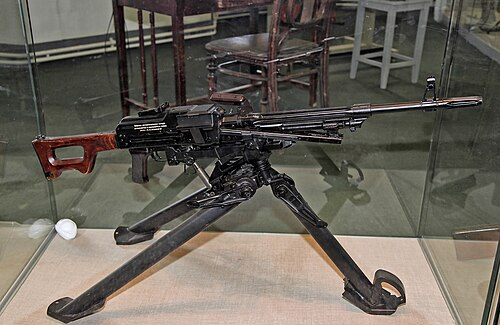
\includegraphics{../images/karabiny_maszynowe/pk_1.jpg}
\caption{PK/PKM --- karabin maszynowy ogólnego przeznaczenia}
\end{figure}

\subsection{Opis}\label{opis-71}

PK (Пулемёт Калашникова --- Karabin maszynowy Kałasznikowa) to radziecka
ogólna broń wsparcia (GPMG) kalibru 7,62×54R mm opracowana przez
Michaiła Kałasznikowa i przyjęta do służby w 1961 roku. PKM (1969) to
zmodernizowana, lżejsza wersja. Zasilany taśmą nabojów o pełnym rynklu
7,62×54R mm (ten sam nabój co karabin snajperski SVD i karabin Moisina)
--- co daje zasięg skuteczny do 1000 m i celny ogień od 800 m. PK/PKM
jest uważany za jeden z najlepszych karabinów maszynowych ogólnego
przeznaczenia w historii --- prosty, niezawodny, lekki (7,5 kg) i
skuteczny. Stosowany przez armie ponad 100 państw; do dziś jest
standardową bronią wsparcia drużyny piechoty w armii rosyjskiej.

\subsection{Dane techniczne}\label{dane-techniczne-71}

\begin{longtable}[]{@{}
  >{\raggedright\arraybackslash}p{(\columnwidth - 2\tabcolsep) * \real{0.5263}}
  >{\raggedright\arraybackslash}p{(\columnwidth - 2\tabcolsep) * \real{0.4737}}@{}}
\toprule\noalign{}
\begin{minipage}[b]{\linewidth}\raggedright
Parametr
\end{minipage} & \begin{minipage}[b]{\linewidth}\raggedright
Wartość
\end{minipage} \\
\midrule\noalign{}
\endhead
\bottomrule\noalign{}
\endlastfoot
Typ & Karabin maszynowy ogólnego przeznaczenia (GPMG) \\
Kraj produkcji & ZSRR / Rosja \\
Rok wprowadzenia & 1961 (PK) / 1969 (PKM) \\
Kaliber & 7,62×54R mm \\
Długość & 1 173 mm \\
Długość lufy & 658 mm \\
Masa (bez taśmy) & 7,5 kg (PKM) \\
Zasilanie & Taśma 100, 200 lub 250 nabojów \\
Szybkostrzelność & 650--750 strz./min \\
Skuteczny zasięg & 1 000 m (ogień ciągły) / 1 500 m (ogień
bezpośredni) \\
\end{longtable}

\subsection{Charakterystyczne cechy
rozpoznawcze}\label{charakterystyczne-cechy-rozpoznawcze-71}

\begin{quote}
Jak odróżnić PKM od RPK, RPD i NSV:
\end{quote}

\begin{itemize}
\tightlist
\item
  \textbf{Taśma nabojów 7,62×54R zamiast magazynka --- kluczowy
  identyfikator:} PKM jest zasilany metalową taśmą nabojów (100--250
  sztuk w skrzynce); żaden RPK nie ma taśmy --- jeśli broń jest zasilana
  taśmą, to nie jest RPK
\item
  \textbf{Charakterystyczna składana trójnóg lub dwójnóg --- masywna
  metalowa konstrkcja:} PKM ma stalowy składany dwójnóg zamontowany w
  połowie lufy; masywniejszy i dłuższy niż dwójnóg RPK; na trójnogu SPP
  --- wyraźnie cięższy zestaw
\item
  \textbf{Zmieniana lufa --- widoczna dźwignia zwalniająca:} PKM ma
  szybkozmienna lufę --- po lewej stronie komory zamkowej widoczna jest
  dźwignia zwalniająca lufę; wymiana lufy to charakterystyczna operacja
  obsługi PKM widoczna na filmach
\item
  \textbf{Klapka podajnika taśmy na górze komory zamkowej:} na górze
  komory zamkowej PKM widnieje charakterystyczna duża klapka z
  mechanizmem podajnika taśmy; jest szersza i bardziej wypukła niż
  klapka AKM
\item
  \textbf{Prosta, nieregulowana kolba skrzynkowa (drewniana lub
  plastikowa):} kolba PKM jest prosta, nieregulowana, z
  charakterystycznym otworem / skrzynkowym kształtem --- inna od smukłej
  kolby AKM i wyraźnie odróżnia PKM od zachodniej broni wsparcia
\item
  \textbf{Lżejszy i krótszy od NSV i Kord:} NSV i Kord to ciężkie km
  12,7 mm montowane na pojazdach; PKM jest wyraźnie mniejszy i lżejszy;
  przy porównaniu gabaryty NSV są dwa razy większe
\end{itemize}

\subsection{Ciekawostka}\label{ciekawostka-71}

\begin{quote}
PKM stał się symbolem partyzantów i nieregularnych sił zbrojnych na
całym świecie --- co jest paradoksem, bo projektowany był dla regularnej
armii. Afgańscy mudżahedini, hezbollahczycy, żołnierze ISIL i setki
innych podmiotów zbrojnych używali PKM, bo jest lekki i bardzo
wytrzymały. Taliban zdobywał PKM od wojsk radzieckich w Afganistanie ---
i do 2001 roku posiadał więcej PKM niż radziecka armia miała planów.
Najsłynniejsze zdjęcie PKM to karabin zamontowany na dachu pickupa ---
``techniczny'' z PKM to pół-standardowy pojazd bojowy w Afryce i na
Bliskim Wschodzie.
\end{quote}

\section{Karabin maszynowy PKP
Pieczenieg}\label{karabin-maszynowy-pkp-pieczenieg}

\subsubsection{PKP Pecheneg Machine Gun \textbar{} ПКП
«Печенег»}\label{pkp-pecheneg-machine-gun-ux43fux43aux43f-ux43fux435ux447ux435ux43dux435ux433}

\begin{center}\rule{0.5\linewidth}{0.5pt}\end{center}

\begin{figure}
\centering
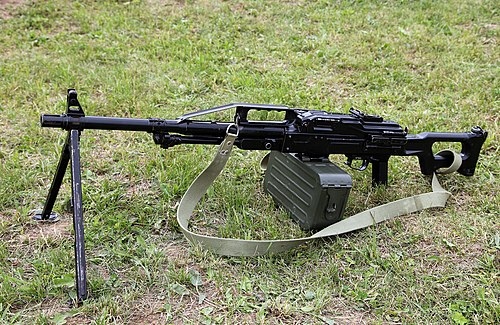
\includegraphics{../images/karabiny_maszynowe/pkp_1.jpg}
\caption{PKP Pieczenieg --- karabin maszynowy}
\end{figure}

\subsection{Opis}\label{opis-72}

PKP Pieczenieg (Печенег --- Pieczyngowie, lud koczowniczy) to rosyjski
ciężki karabin maszynowy ogólnego przeznaczenia kalibru 7,62×54R mm
opracowany przez TsNIITochMash i przyjęty do służby w 1999 roku jako
modernizacja PKM. Wyróżnia się systemem wymuszonego chłodzenia lufy
przez kanał wewnętrzny --- gorące gazy z komory zamkowej cyrkulują wokół
lufy, chłodząc ją bez demontażu; pozwala to na oddanie do 600 nabojów
bez wymiany lufy (PKM wymaga wymiany co 250--300 nabojów). Pieczenieg
nie ma możliwości szybkiej wymiany lufy (i nie potrzebuje jej dzięki
chłodzeniu). Stosowany przez rosyjskie siły specjalne, Spetsnaz i
jednostki szturmowe.

\subsection{Dane techniczne}\label{dane-techniczne-72}

\begin{longtable}[]{@{}ll@{}}
\toprule\noalign{}
Parametr & Wartość \\
\midrule\noalign{}
\endhead
\bottomrule\noalign{}
\endlastfoot
Typ & Karabin maszynowy ogólnego przeznaczenia \\
Kraj produkcji & Rosja \\
Rok wprowadzenia & 1999 \\
Kaliber & 7,62×54R mm \\
Długość & 1 155 mm \\
Długość lufy & 658 mm \\
Masa (bez taśmy) & 8,2 kg \\
Zasilanie & Taśma 100, 200 lub 250 nabojów \\
Szybkostrzelność & 650--750 strz./min \\
Skuteczny zasięg & 1 500 m \\
\end{longtable}

\subsection{Charakterystyczne cechy
rozpoznawcze}\label{charakterystyczne-cechy-rozpoznawcze-72}

\begin{quote}
Jak odróżnić PKP Pieczenieg od PKM:
\end{quote}

\begin{itemize}
\tightlist
\item
  \textbf{Grubsza, ciężka lufa bez możliwości wymiany w polu:} lufa
  Pieczeniega jest wyraźnie grubsza od lufy PKM --- o cięższym profilu i
  z radiatorowymi żebrami; na PKM lufa jest smuklejsza i cieńsza; ta
  grubość jest kluczową cechą wizualną
\item
  \textbf{Brak dźwigni szybkiej wymiany lufy:} PKM ma wyraźną dźwignię
  zwalniającą lufę po lewej stronie komory zamkowej; Pieczenieg jej nie
  ma --- jego gruba lufa nie jest wymienialna; przy obejrzeniu z boku
  brak tej dźwigni natychmiast odróżnia broń
\item
  \textbf{Uchwyt przedni pionowy pod lufą (bipod jest tu przeniesiony):}
  Pieczenieg ma charakterystyczny pionowy uchwyt przedni (foregrip) pod
  lufą; PKM go nie ma; ten uchwyt to bardzo wyraźna cecha wizualna,
  widoczna natychmiast
\item
  \textbf{Charakterystyczna osłona lufy (heat shield) wzdłuż całej
  lufy:} nad lufą Pieczeniega widnieje metalowa osłona cieplna na całej
  długości --- pozwala na przytrzymanie broni za lufę bez poparzenia;
  PKM nie ma takiej osłony (lufa PKM jest odsłonięta)
\item
  \textbf{Dwójnóg przesunięty w kierunku komory (bardziej do tyłu niż w
  PKM):} dwójnóg Pieczeniega jest zamontowany bliżej środka ciężkości
  broni niż w PKM; subtelna różnica w pozycji dwójnogu
\item
  \textbf{Cięższy o 0,7 kg od PKM --- widoczna solidniejsza bryła:}
  Pieczenieg waży 8,2 kg vs 7,5 kg PKM; przy porównaniu na oko różnica
  nie jest dramatyczna, ale sylwetka Pieczeniega jest ``solidniejsza'' i
  bardziej ``wypełniona''
\end{itemize}

\subsection{Ciekawostka}\label{ciekawostka-72}

\begin{quote}
Nazwa ``Pieczenieg'' pochodzi od koczowniczego ludu stepowego, który
przez wieki napadał na Ruś Kijowską. Konstruktorzy wybrali tę nazwę, bo
--- ich zdaniem --- nowy km miał być tak nieustępliwy w walce jak
starożytni Pieczyngowie. W Czeczenii Pieczenieg zaskoczył rosyjskich
żołnierzy: podczas długich zasadzek mogli prowadzić nieprzerwany ogień
przez kilkadziesiąt minut bez chłodzenia, podczas gdy obsługi PKM co
kilkanaście minut musiały wymieniać lufy lub przerywać ogień. To
pierwsza ``cold barrel advantage'' dla rosyjskiego km od czasów
Degtiariewa.
\end{quote}

\section{Ciężki karabin maszynowy
DszkK}\label{ciux119ux17cki-karabin-maszynowy-dszkk}

\subsubsection{DShK Heavy Machine Gun \textbar{} ДШК (Дегтярёв-Шпагин
Крупнокалиберный)}\label{dshk-heavy-machine-gun-ux434ux448ux43a-ux434ux435ux433ux442ux44fux440ux451ux432-ux448ux43fux430ux433ux438ux43d-ux43aux440ux443ux43fux43dux43eux43aux430ux43bux438ux431ux435ux440ux43dux44bux439}

\begin{center}\rule{0.5\linewidth}{0.5pt}\end{center}

\begin{figure}
\centering
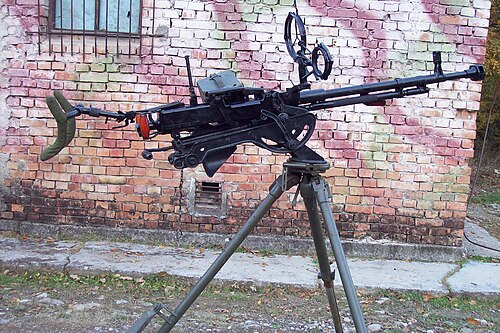
\includegraphics{../images/karabiny_maszynowe/dshk_1.jpg}
\caption{DShK --- ciężki karabin maszynowy 12,7 mm}
\end{figure}

\subsection{Opis}\label{opis-73}

DShK (Дегтярёв-Szpagin Крупнокалиберный) to radziecki ciężki karabin
maszynowy kalibru 12,7×108 mm zaprojektowany przez Wasilija Diegtiarjewa
i Gieorgija Szpagina i przyjęty do służby w 1938 roku. Pomimo wieku
ponad 85 lat DShK jest nadal w aktywnej służbie w dziesiątkach armii i
ruchów zbrojnych na całym świecie --- od Afganistanu przez Afrykę po
Ukrainę. Używa potężnego naboju 12,7×108 mm zdolnego do rażenia lekkich
pojazdów opancerzonych, helikopterów i umocnień na odległość do 2000 m.
DShK jest montowany na trójnodze naziemnym, pojazdach (technicals,
opancerzone pojazdy) i wieżyczkach morskich. Zmodernizowana wersja DShKM
(1946) jest do dziś produkowana w Chinach, Iranie i innych krajach.

\subsection{Dane techniczne}\label{dane-techniczne-73}

\begin{longtable}[]{@{}
  >{\raggedright\arraybackslash}p{(\columnwidth - 2\tabcolsep) * \real{0.5263}}
  >{\raggedright\arraybackslash}p{(\columnwidth - 2\tabcolsep) * \real{0.4737}}@{}}
\toprule\noalign{}
\begin{minipage}[b]{\linewidth}\raggedright
Parametr
\end{minipage} & \begin{minipage}[b]{\linewidth}\raggedright
Wartość
\end{minipage} \\
\midrule\noalign{}
\endhead
\bottomrule\noalign{}
\endlastfoot
Typ & Ciężki karabin maszynowy (HMG) \\
Kraj produkcji & ZSRR \\
Rok wprowadzenia & 1938 (DShKM: 1946) \\
Kaliber & 12,7×108 mm \\
Długość & 1 626 mm \\
Długość lufy & 1 070 mm \\
Masa (bez trójnogu) & 34 kg \\
Zasilanie & Taśma 50 lub 250 nabojów \\
Szybkostrzelność & 600 strz./min \\
Skuteczny zasięg & 2 000 m (cele naziemne) / 1 500 m (cele
powietrzne) \\
\end{longtable}

\subsection{Charakterystyczne cechy
rozpoznawcze}\label{charakterystyczne-cechy-rozpoznawcze-73}

\begin{quote}
Jak odróżnić DShK od NSV i Kord:
\end{quote}

\begin{itemize}
\tightlist
\item
  \textbf{Bardzo masywny i długi --- wyraźnie archaiczna, gruba
  sylwetka:} DShK ma charakterystyczną grubą, masywną lufę z wyraźnymi
  żebrami chłodzącymi (wzdłużne rowki na lufie); NSV i Kord mają
  gładsze, cieńsze lufy --- DShK wygląda ``artyleryjsko'' i ciężko
\item
  \textbf{Żebra chłodzące na lufie --- widoczne prążki wzdłuż lufy:}
  najbardziej charakterystyczna cecha DShK: wyraźne poziome lub podłużne
  żebra na lufie; NSV ma lufę gładką lub z minimalnym profilowaniem;
  żebra DShK są widoczne nawet na zdjęciach z odległości
\item
  \textbf{Duży okrągły hamulec wylotowy w kształcie ``grzybka'':} DShKM
  ma charakterystyczny okrągły, stożkowy lub ``grzybkowy'' hamulec
  wylotowy; Kord ma bardziej nowoczesny kanciasty hamulec; NSV --- inny
  kształt
\item
  \textbf{Kołowy lawet artyleryjski z dużymi stalowymi kołami:} DShK
  może być montowany na kołowym lawecie z dużymi stalowymi kołami ---
  archaiczny wygląd ``artylerii polowej'' ze stalowymi szprychami; NSV i
  Kord mają nowocześ­niejsze trójnogi bez kół
\item
  \textbf{Podajnik taśmy wychodzący z lewej strony --- wyraźny
  ``garb'':} podajnik boczny DShKM (z 1946 roku) wychodzi z lewej strony
  komory zamkowej jako charakterystyczny ``garb'' podajnikowy; pierwsza
  wersja DShK 1938 miała bębniany podajnik obrotowy
\item
  \textbf{Masywny trójnóg z rozkładanymi nogami --- ``pajęczy''
  kształt:} trójnóg DShK ma charakterystyczne trzy grube nogi rozkładane
  na boki w kształcie gwiazdy; całość wygląda jak ciężka platforma
  artyleryjska, nie jak przenośna broń
\end{itemize}

\subsection{Ciekawostka}\label{ciekawostka-73}

\begin{quote}
DShK był jedną z pierwszych broni zdolnych do skutecznego strącania
samolotów --- i jedna z jego pierwszych ofiar to był\ldots{} własny
samolot radziecki. W 1941 roku radzieccy żołnierze strzelali do
wszystkiego, co latało, bo nie mieli opracowanej procedury
identyfikacji; zestrzelono kilka własnych bombowców SB. DShK ocalał w
służbie dzięki chińskiej kopii (Typ 54) --- Chiny wyprodukowały setki
tysięcy egzemplarzy i sprzedawały je wszędzie; dziś DShK na
``technicalu'' to symbol wojen zastępczych zimnowojennych i
postzimnowojennch w Afryce i Azji.
\end{quote}

\section{Ciężki karabin maszynowy
NSW}\label{ciux119ux17cki-karabin-maszynowy-nsw}

\subsubsection{NSV Heavy Machine Gun \textbar{} НСВ «Утёс»
(Utes)}\label{nsv-heavy-machine-gun-ux43dux441ux432-ux443ux442ux451ux441-utes}

\begin{center}\rule{0.5\linewidth}{0.5pt}\end{center}

\begin{figure}
\centering
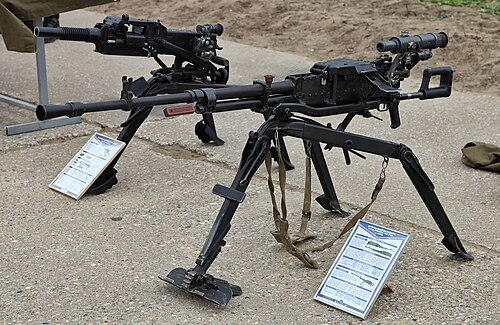
\includegraphics{../images/karabiny_maszynowe/nsv_1.jpg}
\caption{NSW Utes --- ciężki karabin maszynowy 12,7 mm}
\end{figure}

\subsection{Opis}\label{opis-74}

NSW (НСВ --- Nikitin-Sokolov-Wołkow) Utes (Утёс --- Klif) to radziecki
ciężki karabin maszynowy kalibru 12,7×108 mm opracowany przez Nikitin,
Sokołow i Wołkow i przyjęty do służby w 1971 roku jako następnik DShKM.
NSW był znacznie lżejszy od DShKM (25 kg vs 34 kg) i bardziej nowoczesny
--- zredukowana masa pozwoliła na szersze stosowanie go na wieżyczkach
pojazdów opancerzonych (T-72, T-80, T-90, BMP-3). Poza rolą
przeciwpancerną (lekkie pancerze do 16 mm) NSW jest skuteczny przeciwko
śmigłowcom i piechurze w zasięgu do 2000 m. Szeroko stosowany przez
armie postsowieckie; wycofywany z rosyjskiej służby na rzecz Kord, ale
wciąż powszechny.

\subsection{Dane techniczne}\label{dane-techniczne-74}

\begin{longtable}[]{@{}ll@{}}
\toprule\noalign{}
Parametr & Wartość \\
\midrule\noalign{}
\endhead
\bottomrule\noalign{}
\endlastfoot
Typ & Ciężki karabin maszynowy (HMG) \\
Kraj produkcji & ZSRR / Rosja \\
Rok wprowadzenia & 1971 \\
Kaliber & 12,7×108 mm \\
Długość & 1 560 mm \\
Długość lufy & 1 100 mm \\
Masa (bez trójnogu) & 25 kg \\
Zasilanie & Taśma 50 nabojów \\
Szybkostrzelność & 700--800 strz./min \\
Skuteczny zasięg & 2 000 m \\
\end{longtable}

\subsection{Charakterystyczne cechy
rozpoznawcze}\label{charakterystyczne-cechy-rozpoznawcze-74}

\begin{quote}
Jak odróżnić NSW od DShK i Kord:
\end{quote}

\begin{itemize}
\tightlist
\item
  \textbf{Gładka lufa bez żeber chłodzących --- w odróżnieniu od DShK:}
  NSW ma stosunkowo gładką lufę (bez wyraźnych żeber); DShK ma
  charakterystyczne żebra wzdłuż całej lufy; ta gładkość NSV jest
  pierwszą wskazówką przy identyfikacji
\item
  \textbf{Charakterystyczny podajnik taśmy z lewej --- okrągły
  mechanizm:} mechanizm podajnika NSV jest okrągły lub owoidalny z lewej
  strony komory zamkowej --- wyraźny ``guz'' boczny; mniej
  charakterystyczny niż skrzynkowy podajnik DShKM
\item
  \textbf{Mniejszy i lżejszy od DShK --- wyraźnie smuklejsza bryła:} NSV
  jest o 9 kg lżejszy od DShK; wizualnie jest smuklejszy i krótszy; przy
  porównaniu obu broni NSV sprawia wrażenie bardziej ``elegancki'' i
  nowocześniejszy
\item
  \textbf{Często widoczny na wieżyczkach T-72/T-80/T-90 --- jako km
  przeciwlotniczy:} NSW jest standardowym km przeciwlotniczym montowanym
  na wieżyczkach czołgów T-72 i T-80; na szczycie wieżyczki czołgu
  widoczna charakterystyczna pionowa lufa NSV --- to ``flaga''
  rozpoznawcza
\item
  \textbf{Trójnóg NSP-12 z rozkładanymi nogami:} NSV jest montowany na
  nowoczesnym stalowym trójnogu z regulacją wysokości; lżejszy i
  nowocześniejszy od kołowego lawetu DShK
\item
  \textbf{Szybkostrzelność wyższa niż DShK --- słyszalna różnica w
  rytmie:} NSV strzela szybciej (700--800 strz./min) niż DShK (600
  strz./min); przy nasłuchu różnica w rytmie ognia jest wyczuwalna przez
  doświadczonych obserwatorów
\end{itemize}

\subsection{Ciekawostka}\label{ciekawostka-74}

\begin{quote}
NSW był pierwszym sowieckim ciężkim km, który nie pochodził z ``fabryki
Degtiariewa'' --- łamiąc monopol, który Diegtiariów miał na sowiecką
broń wsparcia od 1926 roku. Kiedy prototyp NSW przeszedł testy, mówiono
żartem, że ``Degtiariów skręcił się w grobie'' --- choć konstruktor żył
do 1949 roku. NSW zdominował wieżyczki czołgów rosyjskich do tego
stopnia, że na Ukrainie żołnierze szybko nauczyli się zdejmować NSV ze
zniszczonych rosyjskich czołgów i montować je na własnych pojazdach ---
gotowa ciężka broń wsparcia bez żadnej adaptacji.
\end{quote}

\section{Ciężki karabin maszynowy
Kord}\label{ciux119ux17cki-karabin-maszynowy-kord}

\subsubsection{Kord Heavy Machine Gun \textbar{} Корд
(6П50)}\label{kord-heavy-machine-gun-ux43aux43eux440ux434-6ux43f50}

\begin{center}\rule{0.5\linewidth}{0.5pt}\end{center}

\begin{figure}
\centering
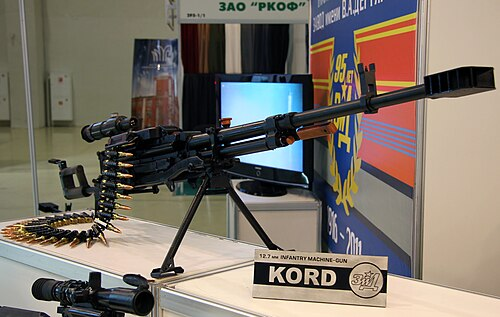
\includegraphics{../images/karabiny_maszynowe/kord_1.jpg}
\caption{Kord --- ciężki karabin maszynowy 12,7 mm}
\end{figure}

\subsection{Opis}\label{opis-75}

Kord (6П50) to rosyjski ciężki karabin maszynowy kalibru 12,7×108 mm
opracowany przez ZID (Zawod im. Diegtiarjewa) w Kowrowie i przyjęty do
służby w 1998 roku jako następnik NSV. Jest znacznie lżejszy od NSV
dzięki ulepszonej konstrukcji lufy ze specjalnym systemem odprowadzania
gazów --- masa Kord to tylko 25,5 kg (porównywalna z NSV), ale kluczową
różnicą jest możliwość strzelania z dwójnogu bez trójnogu przez jednego
żołnierza (w pewnych warunkach) --- czego DShK ani NSV nie potrafią.
Kord jest standardowym ciężkim km montowanym na wieżyczkach T-90M, T-14
Armata, BMP-3M i wielu innych pojazdach rosyjskich.

\subsection{Dane techniczne}\label{dane-techniczne-75}

\begin{longtable}[]{@{}ll@{}}
\toprule\noalign{}
Parametr & Wartość \\
\midrule\noalign{}
\endhead
\bottomrule\noalign{}
\endlastfoot
Typ & Ciężki karabin maszynowy (HMG) \\
Kraj produkcji & Rosja \\
Rok wprowadzenia & 1998 \\
Kaliber & 12,7×108 mm \\
Długość & 1 980 mm \\
Długość lufy & 1 070 mm \\
Masa (bez trójnogu) & 25,5 kg \\
Zasilanie & Taśma 50 nabojów \\
Szybkostrzelność & 650--750 strz./min \\
Skuteczny zasięg & 2 000 m \\
\end{longtable}

\subsection{Charakterystyczne cechy
rozpoznawcze}\label{charakterystyczne-cechy-rozpoznawcze-75}

\begin{quote}
Jak odróżnić Kord od NSW i DShK:
\end{quote}

\begin{itemize}
\tightlist
\item
  \textbf{Nowoczesny, kanciasty hamulec wylotowy w kształcie
  ``skrzynki'':} Kord ma charakterystyczny prostokątny wielokomorowy
  hamulec wylotowy --- kanciasty, nowoczesny wygląd; DShK ma okrągły
  ``grzybkowy'' hamulec, NSV --- inny kształt; hamulec Kord jest od razu
  rozpoznawalny jako ``inny''
\item
  \textbf{Wyraźnie dłuższy od NSV --- o ok. 40 cm:} Kord ma lufę 107 cm
  i długość całkowitą ok. 198 cm --- jest wyraźnie dłuższy od NSV (156
  cm); proporcje Kord są bardziej ``armatnie'' i rozciągnięte
\item
  \textbf{Nowoczesne łoże i chwyt pistoletowy z prawej:} Kord ma
  nowoczesny ergonomiczny chwyt pistoletowy (jak karabin szturmowy)
  zamiast tradycyjnych rękojeści; to bardzo wyraźna cecha --- DShK i NSV
  mają klasyczne ``uszate'' uchwyty
\item
  \textbf{Charakterystyczna pełna osłona lufy z otworami:} nad lufą Kord
  widnieje charakterystyczna metalowa osłona z wyciętymi otworami
  wentylacyjnymi --- estetycznie nowoczesna; DShK i NSV nie mają takiej
  osłony lufy
\item
  \textbf{Montaż na T-90M i T-14 Armata --- na nowoczesnych czołgach:}
  jeśli ciężki km jest widoczny na szczycie wieżyczki T-90M lub T-14
  Armata --- to prawie na pewno Kord; NSV jest na starszych T-72/T-80;
  DShK na jeszcze starszych pojazdach
\item
  \textbf{Charakterystyczny układ podajnika --- skrzynka z boku (prawa
  strona):} Kord ładuje taśmę z prawej strony (NSV --- lewa); ta różnica
  w stronę podawania taśmy jest dobrym wyróżnikiem przy obserwacji
  obsługi broni
\end{itemize}

\subsection{Ciekawostka}\label{ciekawostka-75}

\begin{quote}
Kord był pierwszą radziecko-rosyjską bronią ciężką, która mogła być
teoretycznie obsługiwana przez jedną osobę w polu --- bez rozkładania
trójnogu, przez krótkie serie z dwójnogu lub z biodra (choć jest to
niecelne i ``akrobatyczne''). Zaprezentowano to na pokazach, wywołując
niedowierzanie --- przecież DShK ważył 34 kg na trójnogu i potrzebował 4
ludzi do przeniesienia. Kord ze stopą naramienną i dwójnogiem mógł
teoretycznie obsługiwać jeden silny żołnierz --- choć w praktyce i tak
się tego nie robi ze względu na odrzut i celność.
\end{quote}

\section{Karabin snajperski VSS
Wintorez}\label{karabin-snajperski-vss-wintorez}

\subsubsection{VSS Vintorez Sniper Rifle \textbar{} ВСС
«Винторез»}\label{vss-vintorez-sniper-rifle-ux432ux441ux441-ux432ux438ux43dux442ux43eux440ux435ux437}

\begin{center}\rule{0.5\linewidth}{0.5pt}\end{center}

\begin{figure}
\centering
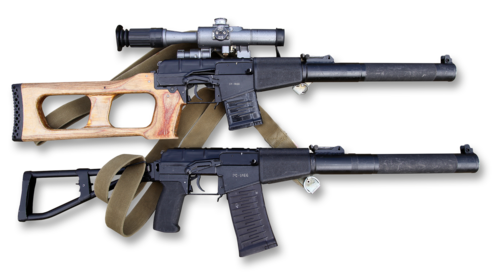
\includegraphics{../images/karabiny_snajperskie/vss_1.jpg}
\caption{VSS Wintorez --- tłumiony karabin snajperski}
\end{figure}

\subsection{Opis}\label{opis-76}

VSS Wintorez (Винторез --- Gwintownik) to radziecki tłumiony karabin
snajperski kalibru 9×39 mm opracowany przez TsNIITochMash i przyjęty do
służby w 1987 roku dla KGB, GRU i sił specjalnych. Jest siostrzaną
bronią AS Val --- używa identycznego naboju 9×39 mm i tłumika, ale jest
przeznaczony do precyzyjnego ognia półautomatycznego (nie automatycznego
jak AS Val). Wintorez może być rozkładany w pole i transportowany w
walizce dyplomatycznej lub plecaku w ciągu 60 sekund. Celownik PSO-1-1
lub noktowizyjny NSPU-3 pozwala na celny ogień do 400 m (400 m z celem w
pancerzu klasy III). Stosowany przez GRU, FSB i Spetsnaz; pojawia się w
Czeczenii, Syrii i na Ukrainie.

\subsection{Dane techniczne}\label{dane-techniczne-76}

\begin{longtable}[]{@{}ll@{}}
\toprule\noalign{}
Parametr & Wartość \\
\midrule\noalign{}
\endhead
\bottomrule\noalign{}
\endlastfoot
Typ & Tłumiony karabin snajperski \\
Kraj produkcji & ZSRR / Rosja \\
Rok wprowadzenia & 1987 \\
Kaliber & 9×39 mm \\
Długość & 894 mm \\
Długość lufy & 200 mm \\
Masa (z tłumikiem i bez magazynka) & 2,6 kg \\
Pojemność magazynka & 10 nabojów \\
Prędkość wylotowa & 290--295 m/s (poddźwiękowa) \\
Skuteczny zasięg & 300--400 m \\
\end{longtable}

\subsection{Charakterystyczne cechy
rozpoznawcze}\label{charakterystyczne-cechy-rozpoznawcze-76}

\begin{quote}
Jak odróżnić VSS Wintorez od AS Val i SVD:
\end{quote}

\begin{itemize}
\tightlist
\item
  \textbf{Mały, kompaktowy karabin z dużym zintegrowanym tłumikiem:}
  Wintorez ma tłumik stanowiący niemal połowę długości broni ---
  zintegrowany, nie do demontażu podczas walki; całość jest krótka i
  ``gruba'' z przodu ze względu na tłumik
\item
  \textbf{Wyraźny celownik optyczny na standardowej szynie:} VSS ma
  gniazdo celownika optycznego na górze komory zamkowej; standardowy
  PSO-1-1 lub noktowizyjny NSPU-3; celownik optyczny i tłumik razem ---
  to nie AS Val (który jest bardziej ``automatyczny'')
\item
  \textbf{Mały magazynek 10-nabojowy (wąski):} magazynek VSS na 10
  nabojów 9×39 mm jest krótki i wąski; AS Val używa magazynka
  20-nabojowego; ta różnica w magazynku jest dobrą wskazówką
\item
  \textbf{Drewniana lub składana kolba, ażurowa --- typowo
  ``snajperska'':} kolba VSS ma często drewniany lub plastikowy element
  z charakterystycznym ``okienkiem'' --- wygląd bardziej snajperski niż
  szturmowy; AS Val ma kolbę bardziej kompaktową i wojskową
\item
  \textbf{Zdejmowalna kolba i łoże --- możliwość transportu w walizce:}
  VSS można rozkładać na 3 główne elementy (komora-tłumik, łoże, kolba)
  i spakować do walizki 45×37×14 cm; ta cecha jest unikatowa wśród
  karabinów snajperskich i typowa dla broni ``tajnych służb''
\item
  \textbf{Wyraźnie krótszy i lżejszy od SVD:} SVD ma 1225 mm długości i
  waży 4,3 kg; VSS ma 894 mm i 2,6 kg; przy porównaniu VSS jest
  karabinem ``kieszonkowym'' w stosunku do SVD
\end{itemize}

\subsection{Ciekawostka}\label{ciekawostka-76}

\begin{quote}
VSS Wintorez był przez lata jedną z najbardziej pilnie strzeżonych
tajemnic wojskowych ZSRR. Broń była tak ściśle klasyfikowana, że nawet
rosyjscy żołnierze, którzy jej nie używali, nie wiedzieli o jej
istnieniu. Pierwsza publikacja technicznych szczegółów nastąpiła dopiero
w latach 90. Po ujawnieniu Wintorez stał się pożądanym łupem --- w
Czeczenii mudżahedini i separatyści oferowali za zdobyty egzemplarz VSS
więcej niż za jakąkolwiek inną broń ręczną. Podobno przynajmniej kilka
egzemplarzy trafiło do CIA przez pośredników.
\end{quote}

\section{Karabin snajperski SVD
Dragunow}\label{karabin-snajperski-svd-dragunow}

\subsubsection{SVD Dragunov Sniper Rifle \textbar{} СВД (Снайперская
винтовка
Драгунова)}\label{svd-dragunov-sniper-rifle-ux441ux432ux434-ux441ux43dux430ux439ux43fux435ux440ux441ux43aux430ux44f-ux432ux438ux43dux442ux43eux432ux43aux430-ux434ux440ux430ux433ux443ux43dux43eux432ux430}

\begin{center}\rule{0.5\linewidth}{0.5pt}\end{center}

\begin{figure}
\centering
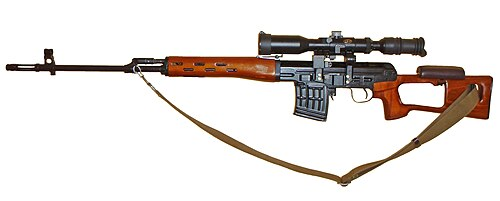
\includegraphics{../images/karabiny_snajperskie/svd_1.jpg}
\caption{SVD Dragunow --- karabin snajperski}
\end{figure}

\subsection{Opis}\label{opis-77}

SVD (Снайперская Винтовка Драгунова --- Snajperski karabin Dragunowa) to
radziecki karabin snajperski kalibru 7,62×54R mm zaprojektowany przez
Jewgienija Dragunowa i przyjęty do służby w 1963 roku. Jest jednym z
najbardziej rozpoznawalnych i powszechnych karabinów snajperskich na
świecie --- produkowany w ponad 30 krajach, stosowany przez armie ponad
50 państw. SVD wyróżnia się gazową automatyką umożliwiającą ogień
półautomatyczny przy zachowaniu celności --- może oddawać 30 strzałów na
minutę bez utraty możliwości snajperskich do 600 m. Standardowy celownik
PSO-1 (4×) pozwala na skuteczny ogień do 1300 m. SVD przez dekady był
standardowym karabinem drużynowego snajpera w całym Układzie Warszawskim
--- w tym w Polsce.

\subsection{Dane techniczne}\label{dane-techniczne-77}

\begin{longtable}[]{@{}ll@{}}
\toprule\noalign{}
Parametr & Wartość \\
\midrule\noalign{}
\endhead
\bottomrule\noalign{}
\endlastfoot
Typ & Karabin snajperski półautomatyczny \\
Kraj produkcji & ZSRR / Rosja \\
Rok wprowadzenia & 1963 \\
Kaliber & 7,62×54R mm \\
Długość & 1 225 mm \\
Długość lufy & 620 mm \\
Masa (bez celownika) & 4,3 kg \\
Pojemność magazynka & 10 nabojów \\
Prędkość wylotowa & 830 m/s \\
Skuteczny zasięg & 800--1 300 m \\
\end{longtable}

\subsection{Charakterystyczne cechy
rozpoznawcze}\label{charakterystyczne-cechy-rozpoznawcze-77}

\begin{quote}
Jak odróżnić SVD od PSL (rumuński) i SV-98:
\end{quote}

\begin{itemize}
\tightlist
\item
  \textbf{Charakterystyczna ``ażurowa'' drewniana lub plastikowa kolba z
  otworem:} kolba SVD ma charakterystyczny otwór w kształcie koła lub
  owalu --- ``ażurowa'' konstrukcja odróżniająca ją od każdej innej
  kolby snajperskiej; ten otwór jest wizualnym znakiem rozpoznawczym SVD
  z 100 metrów
\item
  \textbf{Pistoletowy chwyt oddzielony od kolby --- układ semi-pistol
  grip:} SVD ma klasyczny układ z uchwytem pistoletowym oddzielonym od
  kolby, widocznym pod komorą spustową; SV-98 ma układ burstowy
\item
  \textbf{Celownik PSO-1 (lub PSO-4) na bocznej szynie --- zielony
  metalowy korpus:} standardowy celownik PSO-1 jest charakterystycznym
  zielono-szarym (lub czarnym) metalowym tubusem montowanym na bocznej
  szynie po lewej stronie komory zamkowej; to ikona SVD
\item
  \textbf{Krótkie, wąskie łoże sięgające tylko do połowy lufy:} łoże SVD
  sięga do połowy lufy, zostawiając przednią połowę lufy odsłoniętą;
  charakterystyczna smukłość i długość ``nagiej'' lufy
\item
  \textbf{Mały magazynek 10-nabojowy --- wąski i prawie prosty:}
  magazynek SVD na 10 nabojów 7,62×54R jest wąski i niemal prosty (bo
  nabój z rantem); bardzo inny od zaokrąglonych magazynków AK
\item
  \textbf{Długa, smukła lufa --- proporcjonalnie dłuższa niż AK:} SVD
  jest wyraźnie dłuższy od AKM; smukła długa lufa to cecha
  ``snajperska'' widoczna przy porównaniu z bronią szturmową
\end{itemize}

\subsection{Ciekawostka}\label{ciekawostka-77}

\begin{quote}
SVD jest tak ikonicznym karabinem, że rumuńscy konstruktorzy stworzyli
niemal identyczną kopię PSL --- która mimo identycznego wyglądu nie ma z
SVD żadnej wspólnej części. PSL jest oparty na mechanice RPK, nie SVD.
Skutek? Przez dekady zachodnie wywiady myliły PSL z SVD na zdjęciach
satelitarnych i w raportach. Dopiero po fizycznym zbadaniu obu broni
zorientowano się, że ``dwa SVD'' to dwa zupełnie różne karabiny w
identycznej kamuflażowej sukience.
\end{quote}

\section{Karabin snajperski SV-98}\label{karabin-snajperski-sv-98}

\subsubsection{SV-98 Sniper Rifle \textbar{}
СВ-98}\label{sv-98-sniper-rifle-ux441ux432-98}

\begin{center}\rule{0.5\linewidth}{0.5pt}\end{center}

\begin{figure}
\centering
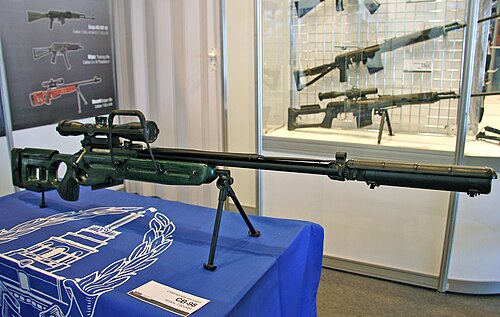
\includegraphics{../images/karabiny_snajperskie/sv-98_1.jpg}
\caption{SV-98 --- karabin snajperski bolt-action}
\end{figure}

\subsection{Opis}\label{opis-78}

SV-98 to rosyjski precyzyjny karabin snajperski kalibru 7,62×54R mm
opracowany przez IZHMASH (dziś Konsorcjum Kałasznikowa) i przyjęty do
służby w 2003 roku. W odróżnieniu od SVD (który jest półautomatyczny i
przeznaczony dla snajpera drużynowego), SV-98 jest bronią stricte
precyzyjną --- powtarzalną (bolt-action) --- przeznaczoną dla
wyszkolonych snajperów wojskowych i antyterrorystycznych. Lufa o
wysokiej dokładności, ciężki profil i łoże z regulowanymi policzkami i
stopką zapewniają celność poniżej 0,5 MOA. Dostępny też w kalibrze .308
Winchester do eksportu. Stosowany przez FSB, Rosyjskie Jednostki
Specjalne i regularną armię; pojawia się regularnie na Ukrainie.

\subsection{Dane techniczne}\label{dane-techniczne-78}

\begin{longtable}[]{@{}ll@{}}
\toprule\noalign{}
Parametr & Wartość \\
\midrule\noalign{}
\endhead
\bottomrule\noalign{}
\endlastfoot
Typ & Karabin snajperski powtarzalny (bolt-action) \\
Kraj produkcji & Rosja \\
Rok wprowadzenia & 2003 \\
Kaliber & 7,62×54R mm (.308 Win w wersji eksportowej) \\
Długość & 1 270 mm \\
Długość lufy & 650 mm \\
Masa (bez celownika) & 5,5 kg \\
Pojemność magazynka & 10 nabojów \\
Prędkość wylotowa & 820 m/s \\
Skuteczny zasięg & 1 000 m (precyzyjny) \\
\end{longtable}

\subsection{Charakterystyczne cechy
rozpoznawcze}\label{charakterystyczne-cechy-rozpoznawcze-78}

\begin{quote}
Jak odróżnić SV-98 od SVD i Orsis T-5000:
\end{quote}

\begin{itemize}
\tightlist
\item
  \textbf{Regulowane łoże z wystającymi policzkiem i stopką ---
  nowoczesna ergonomia:} SV-98 ma charakterystyczne regulowane łoże
  snajperskie z wysuwanym policzkiem i regulowaną stopką kolby ---
  typowy wygląd nowoczesnej precyzyjnej platformy bolt-action; SVD ma
  stałą ażurową kolbę
\item
  \textbf{Masywna ciężka lufa bez gazownika (bolt-action):} SV-98 jest
  powtarzalny (bolt-action) --- nie ma układu gazowego, rury gazowej ani
  gazownika nad lufą; lufa jest grubsza i ``masywniejsza'' niż w SVD;
  brak rury gazowej to kluczowy wyróżnik od SVD
\item
  \textbf{Charakterystyczna szyna Picatinny na górze komory:} SV-98 ma
  standardową szynę Picatinny na górze --- montaż nowoczesnych
  celowników; SVD ma boczną szynę po lewej; ta różnica w lokalizacji
  szyny to ważny identyfikator
\item
  \textbf{Mała rękojeść (bolt handle) wyraźnie z prawej strony:} u broni
  bolt-action widoczna jest charakterystyczna pałka zamkowa z prawej
  strony komory --- wyraźna ``rączka'' zamka; u SVD (półautomatyczny)
  nie ma widocznej pałki zamkowej w tym miejscu
\item
  \textbf{Dwójnóg zamontowany przy komorze nabojowej (dalej od wylotu
  niż w SVD):} SV-98 montuje dwójnóg w środkowej części łoża; SVD jeśli
  ma dwójnóg, to przy wylocie lufy lub go nie ma; pozycja dwójnogu jest
  cechą identyfikującą
\item
  \textbf{Podłużny hamulec wylotowy w kształcie ``walca'':} SV-98 ma
  charakterystyczny cylindryczny lub stożkowy hamulec wylotowy; wyraźnie
  inny od hamulca SVD (jeśli w ogóle jest montowany)
\end{itemize}

\subsection{Ciekawostka}\label{ciekawostka-78}

\begin{quote}
SV-98 zdobył popularność po tym, jak rosyjskie siły specjalne użyły go
podczas oblężenia szkoły w Biesłanie w 2004 roku --- i po raz pierwszy
oficjalnie użyto go w tak nagłośnionej operacji. Dziennikarze
fotografowali rosyjskich specnazowców z charakterystycznym karabinem, co
spowodowało falę zainteresowania tą bronią. Broń wniesiona do Biesłanu
przez terrorystów to były AKS i RPG-7 --- a SV-98 był odpowiedzią po
stronie służb. Zdaniem ekspertów Biesłan ujawnił zarówno siłę, jak i
słabości rosyjskiej taktyki snajperskiej.
\end{quote}

\section{Karabin snajperski Orsis
T-5000}\label{karabin-snajperski-orsis-t-5000}

\subsubsection{Orsis T-5000 Sniper Rifle \textbar{} Орсис
Т-5000}\label{orsis-t-5000-sniper-rifle-ux43eux440ux441ux438ux441-ux442-5000}

\begin{center}\rule{0.5\linewidth}{0.5pt}\end{center}

\begin{figure}
\centering
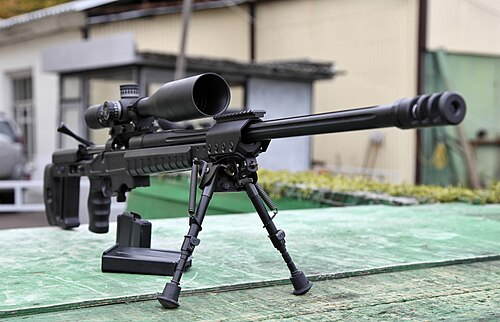
\includegraphics{../images/karabiny_snajperskie/orsis_1.jpg}
\caption{Orsis T-5000 --- precyzyjny karabin snajperski}
\end{figure}

\subsection{Opis}\label{opis-79}

Orsis T-5000 to rosyjski precyzyjny karabin snajperski produkowany przez
prywatną firmę Orsis (Москва) i dostępny w kalibrach .308 Winchester,
.338 Lapua Magnum i 7,62×54R mm. Zaprezentowany w 2011 roku jako
pierwsza w pełni komercyjna rosyjska platforma snajperska klasy premium,
konkurująca z zachodnimi systemami jak Accuracy International AXMC czy
Sako TRX. T-5000 zyskał rozgłos po tym, jak rosyjski snajper Władimir
Onofrijczuk strzelił z niego na igrzyskach olimpijskich w Soczi 2014
(wersja sportowa). Wersja wojskowa jest stosowana przez FSB i wybrane
jednostki specjalne; cywilna wersja sportowa jest popularna w rosyjskich
zawodach snajperskich.

\subsection{Dane techniczne}\label{dane-techniczne-79}

\begin{longtable}[]{@{}ll@{}}
\toprule\noalign{}
Parametr & Wartość \\
\midrule\noalign{}
\endhead
\bottomrule\noalign{}
\endlastfoot
Typ & Precyzyjny karabin snajperski bolt-action \\
Kraj produkcji & Rosja \\
Rok wprowadzenia & 2011 \\
Kaliber & .308 Win / .338 LM / 7,62×54R \\
Długość & 1 290 mm (.308) \\
Długość lufy & 660 mm (.308) \\
Masa (bez celownika) & 6,5 kg \\
Pojemność magazynka & 10 nabojów \\
Prędkość wylotowa & 840 m/s (.308) \\
Skuteczny zasięg & 1 000 m (.308) / 1 500 m (.338 LM) \\
\end{longtable}

\subsection{Charakterystyczne cechy
rozpoznawcze}\label{charakterystyczne-cechy-rozpoznawcze-79}

\begin{quote}
Jak odróżnić Orsis T-5000 od SV-98 i Lobaev Arms:
\end{quote}

\begin{itemize}
\tightlist
\item
  \textbf{Wyraźnie nowoczesne zachodnie wzornictwo --- ``nie wygląda jak
  rosyjski karabin'':} T-5000 jest stylistycznie zbliżony do zachodnich
  platform jak AI AXMC lub Sako --- nowoczesne aluminiowe łoże z
  szynami, regulowane elementy ergonomiczne; znacznie ``zachodniejszy''
  niż SV-98
\item
  \textbf{Aluminiowe łoże chassis z pełnymi szynami Picatinny:} T-5000
  ma charakterystyczne aluminiowe łoże (chassis) --- widoczne boczne
  płyty aluminium; SV-98 i SVD mają konwencjonalne drewniane lub
  plastikowe łoże; ten metaliczny wygląd jest kluczowym identyfikatorem
\item
  \textbf{Regulowana stopka kolby i policzek z wyraźnymi śrubami
  regulacyjnymi:} kolba T-5000 ma wiele możliwości regulacji z
  widocznymi mechanizmami; charakterystyczne ``okucia'' regulacyjne
\item
  \textbf{Charakterystyczny kanciasty hamulec wylotowy Orsis:} T-5000 ma
  rozpoznawalny prostokątny wielokomorowy hamulec wylotowy --- kanciasty
  i masywny; inne kształty niż SV-98 i Lobaev
\item
  \textbf{Rzadkość w terenie --- broń specjalistyczna, nie masowa:}
  T-5000 na Ukrainie lub w strefie konfliktu to rzadkość; jego widok
  sugeruje jednostkę specjalną, nie regularną piechotę
\item
  \textbf{Brak elementów dziedzictwa AK/SVD --- zupełnie inna rodzina
  konstrukcyjna:} T-5000 nie ma żadnych typowych elementów rosyjskiej
  szkoły uzbrojenia; wygląda jak karabin zachodnioeuropejski; ta
  odmienność od klasycznych rosyjskich broni jest sama w sobie
  identyfikatorem
\end{itemize}

\subsection{Ciekawostka}\label{ciekawostka-79}

\begin{quote}
Orsis T-5000 stał się geopolitycznie kontrowersyjny po wprowadzeniu
sankcji po 2014 roku --- firma Orsis importowała kluczowe komponenty
(lufy, mechanizmy zamkowe) z USA i Niemiec, i po sankcjach musiała
przestawić się na produkcję krajową. Rosyjskie media triumfowały, że
``Orsis znalazł krajowe zamienniki'', ale niezależne testy wykazały, że
krajowe lufy są gorsze od importowanych; celność z 0,3 MOA pogorszyła
się do 0,5--0,6 MOA. Mimo to Orsis T-5000 pozostaje symbolem rosyjskich
ambicji w segmencie precyzyjnego uzbrojenia snajperskiego.
\end{quote}

\section{Karabin snajperski KSVK
12,7}\label{karabin-snajperski-ksvk-127}

\subsubsection{KSVK 12.7 Anti-Materiel Rifle \textbar{} КСВК
12,7}\label{ksvk-12.7-anti-materiel-rifle-ux43aux441ux432ux43a-127}

\begin{center}\rule{0.5\linewidth}{0.5pt}\end{center}

\begin{figure}
\centering
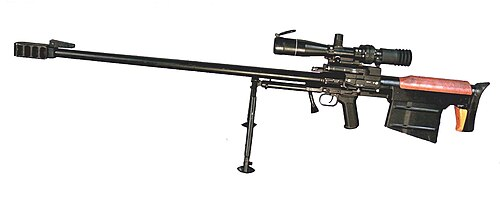
\includegraphics{../images/karabiny_snajperskie/ksvk_1.jpg}
\caption{KSVK 12,7 mm --- wielkokalibrowy karabin snajperski}
\end{figure}

\subsection{Opis}\label{opis-80}

KSVK 12,7 (Крупнокалиберная Снайперская Винтовка Ковровская ---
Wielkokaliberowy karabin snajperski Kowrowski) to rosyjski
wielkokaliberowy karabin snajperski kalibru 12,7×108 mm opracowany przez
ZID w Kowrowie i przyjęty do służby w 2002 roku. Przeznaczony do
niszczenia sprzętu technicznego --- radarów, stacji łączności,
śmigłowców na ziemi, lekkich pojazdów opancerzonych i umocnień --- z
odległości do 1500 m. KSVK jest bronią bolt-action z bultrupsowym
układem (bullpup) --- magazynek i komora zamkowa są za chwytem, co
skraca broń mimo długiej lufy. Stosowany przez rosyjskie siły specjalne
i wojska lądowe; pojawia się na Ukrainie.

\subsection{Dane techniczne}\label{dane-techniczne-80}

\begin{longtable}[]{@{}ll@{}}
\toprule\noalign{}
Parametr & Wartość \\
\midrule\noalign{}
\endhead
\bottomrule\noalign{}
\endlastfoot
Typ & Wielkokaliberowy karabin snajperski / przeciwsprzętowy \\
Kraj produkcji & Rosja \\
Rok wprowadzenia & 2002 \\
Kaliber & 12,7×108 mm \\
Długość & 1 420 mm \\
Długość lufy & 1 000 mm \\
Masa (bez celownika) & 12,5 kg \\
Pojemność magazynka & 5 nabojów \\
Prędkość wylotowa & 850--900 m/s \\
Skuteczny zasięg & 1 500 m (cel techniczny) \\
\end{longtable}

\subsection{Charakterystyczne cechy
rozpoznawcze}\label{charakterystyczne-cechy-rozpoznawcze-80}

\begin{quote}
Jak odróżnić KSVK od OSV-96 i broni .50 BMG:
\end{quote}

\begin{itemize}
\tightlist
\item
  \textbf{Układ bullpup --- magazynek za chwytem pistoletowym:} KSVK ma
  wyraźny bullpup --- chwyt pistoletowy jest daleko z przodu, a
  magazynek jest za chwytem, przy kolbie; OSV-96 ma klasyczny układ ze
  składaną lufą; ta różnica w układzie jest podstawowym identyfikatorem
\item
  \textbf{Bardzo masywna, długa lufa z wielosegmentowym hamulcem:} KSVK
  ma 1-metrową lufę zakończoną ogromnym wielokomorowym hamulcem
  wylotowym --- hamulec jest wyjątkowo duży nawet jak na broń 12,7 mm;
  jego rozmiar wynika z konieczności tłumienia ogromnego odrzutu
\item
  \textbf{Charakterystyczny kształt ``przedłużonej kolby'' bullpup:}
  sylwetka KSVK w układzie bullpup jest charakterystyczna --- długa lufa
  z przodu, krótkie łoże, duży magazynek przy kolbie; ten układ
  proporcji jest inny od wszystkich klasycznych karabinów snajperskich
\item
  \textbf{Kaliber 12,7 mm --- wyraźnie grubszy wylot lufy niż 7,62:}
  otwór wylotowy lufy 12,7 mm jest wyraźnie większy (prawie 1,3 cm) niż
  7,62 mm (0,76 cm); przy bliskim oglądaniu lub na fotografii wyraźna
  różnica w kalibrze
\item
  \textbf{Masywny trójnóg lub specjalny dwójnóg pod łożem:} KSVK strzela
  z trójnogu lub dwójnogu ze względu na masę; specjalny dwójnóg
  montowany pod lufą przy stopce kolby jest charakterystyczną cechą
  broni bullpup tej klasy
\item
  \textbf{Rzadkość --- widoczny tylko w jednostkach specjalnych:} KSVK
  nie jest bronią masową; widok tej broni sugeruje wyspecjalizowaną
  jednostkę snajperską lub siły specjalne; brak w wyposażeniu regularnej
  piechoty
\end{itemize}

\subsection{Ciekawostka}\label{ciekawostka-80}

\begin{quote}
KSVK miał konkurenta w rosyjskim wojsku --- OSV-96 --- i wybór między
nimi toczył się przez lata 2000. W końcu oba przyjęto do służby, bo
miały różne zalety: KSVK (bullpup) jest bardziej kompaktowy i lepszy w
terenie zabudowanym; OSV-96 ma składaną lufę i jest wygodniejszy w
transporcie. Paradoksalnie rosyjskie siły specjalne preferowały KSVK, a
regularni snajperzy dywizyjni --- OSV-96. W efekcie Rosja eksploatuje
dwa bardzo podobne systemy 12,7 mm równolegle --- co logistycy armii
komentują ze zrozumiałą frustracją.
\end{quote}

\section{Karabin snajperski OSV-96}\label{karabin-snajperski-osv-96}

\subsubsection{OSV-96 Anti-Materiel Rifle \textbar{}
ОСВ-96}\label{osv-96-anti-materiel-rifle-ux43eux441ux432-96}

\begin{center}\rule{0.5\linewidth}{0.5pt}\end{center}

\begin{figure}
\centering
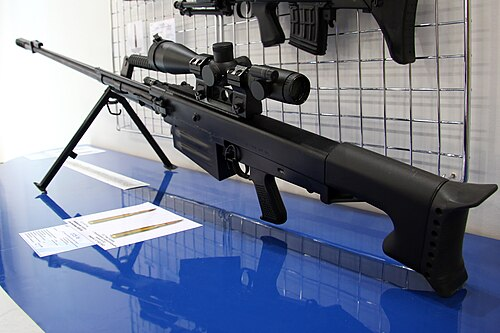
\includegraphics{../images/karabiny_snajperskie/osv-96_1.jpg}
\caption{OSV-96 --- wielkokalibrowy karabin snajperski}
\end{figure}

\subsection{Opis}\label{opis-81}

OSV-96 (Объектовая Снайперская Винтовка --- Obiektowy karabin
snajperski) to rosyjski wielkokaliberowy karabin snajperski kalibru
12,7×108 mm opracowany przez KBP w Tule i przyjęty do służby w 1994
roku. Wyróżnia się mechanizmem składania lufy na pół --- lufa składa się
ku tyłowi nad komorę zamkową, skracając broń z 1746 mm do ok. 1,1 m przy
transporcie; pozwala to na przewożenie go w samochodzie lub śmigłowcu.
OSV-96 jest półautomatyczny (gas-operated) --- może prowadzić ogień
seryjny, co odróżnia go od powtarzalnego KSVK. Stosowany przez rosyjskie
siły specjalne i wojsko lądowe; pojawia się na Ukrainie i w Syrii.

\subsection{Dane techniczne}\label{dane-techniczne-81}

\begin{longtable}[]{@{}ll@{}}
\toprule\noalign{}
Parametr & Wartość \\
\midrule\noalign{}
\endhead
\bottomrule\noalign{}
\endlastfoot
Typ & Wielkokaliberowy karabin snajperski półautomatyczny \\
Kraj produkcji & Rosja \\
Rok wprowadzenia & 1994 \\
Kaliber & 12,7×108 mm \\
Długość (lufa złożona) & \textasciitilde1 100 mm \\
Długość (lufa rozłożona) & 1 746 mm \\
Długość lufy & 1 000 mm \\
Masa (bez celownika) & 12,9 kg \\
Pojemność magazynka & 5 nabojów \\
Prędkość wylotowa & 900 m/s \\
Skuteczny zasięg & 1 800 m \\
\end{longtable}

\subsection{Charakterystyczne cechy
rozpoznawcze}\label{charakterystyczne-cechy-rozpoznawcze-81}

\begin{quote}
Jak odróżnić OSV-96 od KSVK i Lobaev SVLK-14S:
\end{quote}

\begin{itemize}
\tightlist
\item
  \textbf{Składana lufa --- broń ``złamana w połowie'' w transporcie:}
  OSV-96 w transporcie wygląda jak karabin złożony na pół; lufa jest
  złożona ku tyłowi nad komorę zamkową; żaden inny karabin snajperski
  12,7 mm nie ma tej cechy; widok złożonego OSV-96 jest natychmiast
  rozpoznawalny
\item
  \textbf{Klasyczny układ --- magazynek przed chwytem pistoletowym (nie
  bullpup):} OSV-96 ma klasyczny układ z uchwytem i magazynkiem z przodu
  --- inaczej niż KSVK (bullpup); przy rozłożonej lufie proporcje są
  typowe dla konwencjonalnego karabinu
\item
  \textbf{Duży hamulec wylotowy cylinder-klatkowy na końcu długiej
  lufy:} OSV-96 ma charakterystyczny duży cylindryczny lub klatkowy
  hamulec wylotowy; jego kształt jest inny od hamulców KSVK i Lobaev
\item
  \textbf{Półautomatyczny --- widoczna rura gazowa nad lufą:} OSV-96
  jest gaz-operated (semi-auto) --- ma charakterystyczną rurę gazową
  biegnącą nad lufą, jak karabin szturmowy; KSVK (bolt-action) nie ma
  rury gazowej
\item
  \textbf{Masywny stalowy dwójnóg montowany pod środkiem lufy:} dwójnóg
  OSV-96 jest bardzo masywny i montowany przy środku długiej lufy;
  rozkładane nogi stalowe z wyraźnymi ``łokciami'' --- widoczny już z
  odległości
\item
  \textbf{Bardzo duże rozmiary przy rozłożonej lufie --- prawie 1,75 m:}
  rozłożony OSV-96 ma prawie 1,75 m długości; obsługujący go żołnierz
  wydaje się przy nim małoskalowy; ta długość jest natychmiast
  zauważalna
\end{itemize}

\subsection{Ciekawostka}\label{ciekawostka-81}

\begin{quote}
OSV-96 stał się znany w Polsce za sprawą kontrowersyjnego zdarzenia z
1995 roku: rosyjski agent wywiadu próbował przemycić rozkładany OSV-96
przez Warszawę w walizce dyplomatycznej (zasłyszane z wywiadowczych
źródeł polskich --- nieoficjalne). Mechanizm składania lufy sprawia
bowiem, że rozkładany OSV-96 wchodzi do typowej twardej walizki
podróżnej --- co było jedną z cech eksploatowanych przez rosyjskie
służby. Szczegóły zdarzenia nigdy nie zostały oficjalnie potwierdzone
przez żadną ze stron.
\end{quote}

\section{Karabin snajperski Lobaev SVLK-14S
Sumrak}\label{karabin-snajperski-lobaev-svlk-14s-sumrak}

\subsubsection{Lobaev SVLK-14S Sumrak Extreme Long Range Rifle
\textbar{} Лобаев СВЛК-14С
«Сумрак»}\label{lobaev-svlk-14s-sumrak-extreme-long-range-rifle-ux43bux43eux431ux430ux435ux432-ux441ux432ux43bux43a-14ux441-ux441ux443ux43cux440ux430ux43a}

\begin{center}\rule{0.5\linewidth}{0.5pt}\end{center}

\begin{figure}
\centering
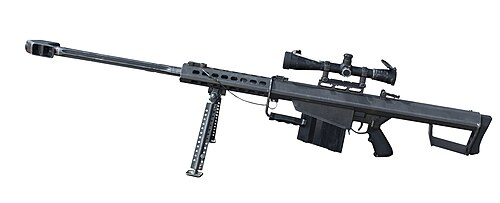
\includegraphics{../images/karabiny_snajperskie/lobaev_1.jpg}
\caption{Lobaev SVLK-14S --- karabin dalekiego zasięgu}
\end{figure}

\subsection{Opis}\label{opis-82}

SVLK-14S Sumrak (Сумрак --- Zmierzch) to rosyjski ekstremalnie
dalekosiężny karabin snajperski opracowany przez Lobaev Arms (Moskwa)
jako platforma do strzelania długodystansowego na odległości ponad 2000
m. Dostępny w kalibrach .408 Cheyenne Tactical i .375 CheyTac --- naboje
ekstremalnie dalekosiężne niestosowane w standardowej służbie wojskowej.
SVLK-14S uzyskał rosyjski rekord odległości strzału: 4210 m (2019 rok,
uderzenie w cel) --- jest to jednocześnie jeden z najdłuższych
potwierdzonych strzałów snajperskich w historii. Broń nie jest
standardową bronią wojskową --- to platforma specjalistyczna dla
wybranych jednostek i ewentualnie do zastosowań dywersyjnych.

\subsection{Dane techniczne}\label{dane-techniczne-82}

\begin{longtable}[]{@{}ll@{}}
\toprule\noalign{}
Parametr & Wartość \\
\midrule\noalign{}
\endhead
\bottomrule\noalign{}
\endlastfoot
Typ & Ekstremalnie dalekosiężny karabin snajperski bolt-action \\
Kraj produkcji & Rosja \\
Rok wprowadzenia & ok. 2015 \\
Kaliber & .408 CheyTac / .375 CheyTac \\
Długość & \textasciitilde1 500 mm \\
Długość lufy & 813 mm (.408) \\
Masa (bez celownika) & ok. 9 kg \\
Pojemność magazynka & 5--7 nabojów \\
Prędkość wylotowa & ok. 1 000 m/s \\
Skuteczny zasięg & 2 000--3 000 m (bojowy) / do 4 210 m (rekordowy) \\
\end{longtable}

\subsection{Charakterystyczne cechy
rozpoznawcze}\label{charakterystyczne-cechy-rozpoznawcze-82}

\begin{quote}
Jak odróżnić Lobaev SVLK-14S od Orsis T-5000 i KSVK:
\end{quote}

\begin{itemize}
\tightlist
\item
  \textbf{Chassis aluminiowy w zachodnim stylu --- ``nie wygląda jak
  rosyjska broń'':} SVLK-14S ma nowoczesne aluminiowe chassis z pełnymi
  szynami jak zachodnie platformy precyzyjne; wygląda jak europejski lub
  amerykański karabin dalekiego zasięgu --- bez żadnych cech rosyjskiego
  dziedzictwa uzbrojenia
\item
  \textbf{Bardzo długa, ciężka lufa z agresywnym hamulcem:} lufa 813 mm
  z masywnym wielokomorowym hamulcem wylotowym jest proporcjonalnie
  najdłuższa spośród omawianych; hamulec zajmuje \textasciitilde15\%
  długości lufy --- widoczna ogromna ``głowica'' na końcu
\item
  \textbf{Niestandardowy kaliber .408 lub .375 CheyTac --- zbyt rzadki
  dla standardowego wojska:} widok amunicji przy obsłudze broni ---
  naboje .408 lub .375 CheyTac są znacznie dłuższe i smuklejsze niż 7,62
  mm i 12,7 mm; bardzo charakterystyczny kształt nabojów
\item
  \textbf{Regulowane wszystko --- łoże, stopka, policzek, dwójnóg:}
  SVLK-14S ma wyjątkowo wiele elementów regulacyjnych; wszystkie
  dostosowane do obsługi; charakterystyczne liczne śruby i pokrętła
  regulacyjne widoczne na łożu
\item
  \textbf{Brak jakichkolwiek cech wizualnych standardowej broni
  wojskowej:} jeśli karabin wygląda jak sprzęt sportowy lub cywilny, a
  nie militarny --- i jest ekstremalnie długi --- to najprawdopodobniej
  Lobaev lub podobna platforma
\item
  \textbf{Celownik wielkokalibrowy \textgreater40x lub urządzenia
  pomiarowe:} SVLK-14S jest zwykle wyposażony w bardzo duży celownik
  snajperski (Schmidt\&Bender, Nightforce itp.) i towarzyszący dalmierz
  laserowy --- charakterystyczny duży tubus celownika na broni
\end{itemize}

\subsection{Ciekawostka}\label{ciekawostka-82}

\begin{quote}
W 2019 roku strzelec z Lobaev Arms osiągnął potwierdzony strzał na
odległość 4210 m --- ustanawiając rosyjski rekord i zajmując wysokie
miejsce na liście najdłuższych strzałów snajperskich w historii. Cel o
wymiarach 60×60 cm został trafiony po kilku strzałach korekcyjnych.
Rosyjskie media nagłośniły ten wyczyn jako demonstrację wyższości
rosyjskiej technologii snajperskiej nad zachodnią --- chociaż recenzenci
zagraniczni wskazywali, że rekord kanadyjski z 2017 roku (3540 m z C15
Long Range Sniper Weapon) i rekordowy strzał Tima Fricka (4200 m z .416
Barrett w USA) stały na podobnym poziomie lub wyżej.
\end{quote}

\section{Granatnik przeciwpancerny
RPG-7}\label{granatnik-przeciwpancerny-rpg-7}

\subsubsection{RPG-7 Anti-Tank Grenade Launcher \textbar{}
РПГ-7}\label{rpg-7-anti-tank-grenade-launcher-ux440ux43fux433-7}

\begin{center}\rule{0.5\linewidth}{0.5pt}\end{center}

\begin{figure}
\centering
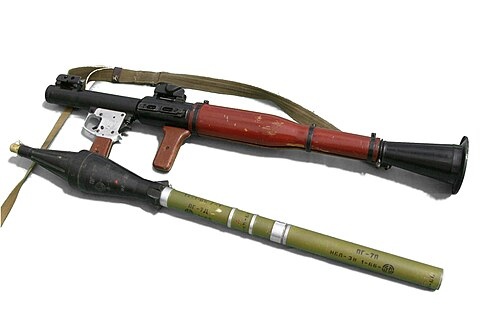
\includegraphics{../images/rpg_wyrzutnie/rpg-7_1.jpg}
\caption{RPG-7 --- granatnik przeciwpancerny}
\end{figure}

\subsection{Opis}\label{opis-83}

RPG-7 to radziecki granatnik przeciwpancerny kalibru 40 mm (lufa) z
naddźwiękowym pociskiem rakietowym o kalibrze 40--105 mm, opracowany
przez GSKB-47 i przyjęty do służby w 1961 roku. Jest najszerzej
stosowanym i produkowanym granatnikiem przeciwpancernym w historii ---
szacunki mówią o ponad 9 milionach egzemplarzy wyprodukownych na całym
świecie. RPG-7 może używać szerokiej gamy głowic: przeciwpancerne
kumulacyjne PG-7 (przebicie 500--750 mm), tandemowe PG-7VR (600 mm za
ERA), termobaryczne TBG-7V, odłamkowe OG-7V i inne. Stosowany przez
armie ponad 40 państw i setki organizacji zbrojnych, bojowników i
milicji na całym świecie; jest symbolem uzbrojenia nieregularnego.

\subsection{Dane techniczne}\label{dane-techniczne-83}

\begin{longtable}[]{@{}
  >{\raggedright\arraybackslash}p{(\columnwidth - 2\tabcolsep) * \real{0.5263}}
  >{\raggedright\arraybackslash}p{(\columnwidth - 2\tabcolsep) * \real{0.4737}}@{}}
\toprule\noalign{}
\begin{minipage}[b]{\linewidth}\raggedright
Parametr
\end{minipage} & \begin{minipage}[b]{\linewidth}\raggedright
Wartość
\end{minipage} \\
\midrule\noalign{}
\endhead
\bottomrule\noalign{}
\endlastfoot
Typ & Granatnik przeciwpancerny wielokrotnego użytku \\
Kraj produkcji & ZSRR / Rosja / wiele innych \\
Rok wprowadzenia & 1961 \\
Kaliber lufy & 40 mm \\
Kaliber pocisku & 40--105 mm (zależnie od głowicy) \\
Długość & 950 mm \\
Masa (bez pocisku) & 6,3 kg \\
Zasięg skuteczny & 200 m (cel ruchomy) / 500 m (cel stały) \\
Przenikanie pancerza & do 750 mm (PG-7VL) / 600 mm za ERA (PG-7VR
tandem) \\
Obsługa & 1--2 osoby \\
\end{longtable}

\subsection{Charakterystyczne cechy
rozpoznawcze}\label{charakterystyczne-cechy-rozpoznawcze-83}

\begin{quote}
Jak odróżnić RPG-7 od RPG-18/22/26 i innych granatników:
\end{quote}

\begin{itemize}
\tightlist
\item
  \textbf{Wielokrotnego użytku --- lufa metalowa, nie jednorazowa:}
  RPG-7 ma trwałą metalową lufę --- nie jest jednorazowa jak RPG-18,
  RPG-22, RPG-26; jeśli strzelec po strzale dalej nosi granatnik --- to
  RPG-7
\item
  \textbf{Charakterystyczna stożkowa lufa rozszerzająca się przy
  wylocie:} tylna część lufy RPG-7 ma charakterystyczny rozszerzony
  stożek (do redukcji odrzutu gazów); ta stożkowa tylnica jest ikoniczna
  --- natychmiast identyfikuje RPG-7
\item
  \textbf{Duży kumulacyjny pocisk wystający z przodu lufy (przed
  strzałem):} przed odpaleniem pocisk PG-7 (lub inny) sterczy znacząco z
  przodu lufy; charakterystyczny kształt głowicy piezoelektrycznej z
  nosem ``iglicowym'' i cylindrycznym ciałem rakiety
\item
  \textbf{Dwuetapowy napęd --- widoczny ślad rakiety po odpaleniu:}
  RPG-7 używa wstępnego ładunku miotającego (wyrzuca pocisk z lufy) i
  silnika rakietowego (odpala się po \textasciitilde10 m);
  charakterystyczny dym i ogień z tyłu przy odpaleniu, potem ślad
  silnika rakietowego
\item
  \textbf{Klasyczny celownik optyczny PGO-7 z lewej strony:} granatnik
  RPG-7 ma charakterystyczny mały celownik optyczny zamontowany po lewej
  stronie lufy --- to najczęstszy układ; rozpoznawalny na zdjęciach jako
  ``mały teleskop na boku granatnika''
\item
  \textbf{Duże, różne typy głowic --- wymienne bez narzędzi:} RPG-7 może
  używać wielu różnych głowic widocznie różniących się kształtem i
  rozmiarem; PG-7 (standardowa) vs TBG-7V (termobaryczna) vs OG-7V
  (odłamkowa) --- każda ma inną sylwetke głowicy
\end{itemize}

\subsection{Ciekawostka}\label{ciekawostka-83}

\begin{quote}
RPG-7 jest wymieniony w Księdze Rekordów Guinnessa jako broń produkowana
przez największą liczbę krajów bez licencji. Prócz ZSRR i Rosji
produkują go lub produkowały: Chiny (Typ 69), Egipt, Iran, Irak,
Rumunia, Bułgaria, Jugosławia i co najmniej 10 innych. Ironicznie ---
USA przez jakiś czas rozważały przyjęcie RPG-7 na uzbrojenie sił
specjalnych jako ``captured enemy equipment'' ze względu na jego
niezawodność i powszechność amunicji. Ostatecznie zdecydowano się na M72
LAW i M3 MAAWS, ale opinia o RPG-7 jako o wyjątkowo niezawodnej broni
pozostaje powszechna wśród wojskowych ekspertów zachodnich.
\end{quote}

\section{Jednorazowy granatnik RPG-18
Mucha}\label{jednorazowy-granatnik-rpg-18-mucha}

\subsubsection{RPG-18 Mukha Disposable Rocket Launcher \textbar{} РПГ-18
«Муха»}\label{rpg-18-mukha-disposable-rocket-launcher-ux440ux43fux433-18-ux43cux443ux445ux430}

\begin{center}\rule{0.5\linewidth}{0.5pt}\end{center}

\begin{figure}
\centering
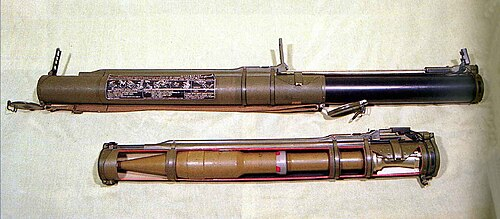
\includegraphics{../images/rpg_wyrzutnie/rpg-18_1.jpg}
\caption{RPG-18 Mucha --- jednorazowy granatnik}
\end{figure}

\subsection{Opis}\label{opis-84}

RPG-18 Mucha (Муха --- Mucha) to radziecki jednorazowy granatnik
przeciwpancerny kalibru 64 mm opracowany przez GSKB-47 i przyjęty do
służby w 1972 roku jako rosyjski odpowiednik amerykańskiego M72 LAW.
Jest prostą, lekką bronią jednorazowego użytku --- po wystrzeleniu
wyrzuca się pustą tubus. Pocisk HEAT przebija do 200 mm pancerza
jednolitego --- wystarczający do rażenia lekkich pojazdów opancerzonych
(BWP, APC, lekkie czołgi), ale niewystarczający do penetracji czołgów z
pancerzem podstawowym. RPG-18 służy jako broń indywidualna żołnierza
piechoty do rażenia lekkich celów opancerzonych i umocnień polowych.
Wycofywany przez nowsze RPG-22, RPG-26, RPG-27, ale wciąż spotykany w
magazynach.

\subsection{Dane techniczne}\label{dane-techniczne-84}

\begin{longtable}[]{@{}ll@{}}
\toprule\noalign{}
Parametr & Wartość \\
\midrule\noalign{}
\endhead
\bottomrule\noalign{}
\endlastfoot
Typ & Jednorazowy granatnik rakietowy (LAW) \\
Kraj produkcji & ZSRR / Rosja \\
Rok wprowadzenia & 1972 \\
Kaliber & 64 mm \\
Długość (złożony) & 705 mm \\
Długość (rozłożony do strzału) & 1 050 mm \\
Masa & 2,6 kg \\
Przenikanie pancerza & 200 mm \\
Zasięg skuteczny & 200 m \\
Obsługa & 1 osoba \\
\end{longtable}

\subsection{Charakterystyczne cechy
rozpoznawcze}\label{charakterystyczne-cechy-rozpoznawcze-84}

\begin{quote}
Jak odróżnić RPG-18 od RPG-22 i RPG-26:
\end{quote}

\begin{itemize}
\tightlist
\item
  \textbf{Cylindryczna, teleskopowa tubus --- rozkładana do strzału:}
  RPG-18 to cylindryczna tubus (jak rura), którą żołnierz rozkłada przed
  strzałem; w złożeniu jest krótka (70 cm), po rozłożeniu --- 105 cm;
  stary, prosty wygląd ``rury'' bez dodatkowych elementów
\item
  \textbf{Mniejszy kaliber 64 mm --- cieńsza rura niż RPG-22 (72 mm):}
  RPG-18 ma kaliber 64 mm vs 72 mm RPG-22; przy bezpośrednim porównaniu
  rura RPG-18 jest cieńsza; to trudne do oceny bez porównania, ale
  istotna różnica techniczna
\item
  \textbf{Brak widocznego celownika optycznego --- prosty przyrząd:}
  RPG-18 ma minimalistyczny celownik (prosty wizjer mechaniczny); RPG-26
  ma bardziej rozbudowany przyrząd celowniczy; prosty celownik to cecha
  starszych typów
\item
  \textbf{Wyraźna archaiczna prostota --- ``stara rura'':} RPG-18
  wygląda jak najstarszy z serii jednorazowych granatników rosyjskich;
  nowsze (RPG-22, 26, 27) mają nowocześniejsze kształty i elementy;
  RPG-18 jest ``retro'' nawet wśród jednorazowych granatników
\item
  \textbf{Jednorazowy --- po strzale wyrzucana pusta tubus:} jak
  wszystkie jednorazowe granatniki --- po strzale tubus jest wyrzucana;
  strzelec nie nosi jej po strzale; charakterystyczna porzucona
  aluminiowa rura na polu walki
\item
  \textbf{Mniejszy i lżejszy od RPG-7 i RPG-29 --- widoczna lekkość:}
  RPG-18 waży 2,6 kg; RPG-7 to 6,3 kg; żołnierz niesie RPG-18 jak lekki
  pakunek; RPG-7 jest wyraźnie większy i masywniejszy
\end{itemize}

\subsection{Ciekawostka}\label{ciekawostka-84}

\begin{quote}
RPG-18 zaprojektowano jako ``broń dla każdego żołnierza'' --- w
odróżnieniu od RPG-7, który wymagał wyszkolenia w obsłudze różnych
głowic i konserwacji. Idea była prosta: dać każdemu żołnierzowi prostą
rurę, którą można wyrzucić bez myślenia. Radzieckie eksperymenty z lat
70. wykazały, że z RPG-18 żołnierz po 15-minutowym szkoleniu mógł trafić
w pojazd z 100 m --- co było wystarczające do walki w warunkach
miejskich. RPG-18 pojawił się szeroko w Afganistanie po obu stronach ---
mudżahedini zdobywali Muchy i używali ich przeciwko radzieckim pojazdom
z zasadzekami.
\end{quote}

\section{Jednorazowy granatnik RPG-22
Netto}\label{jednorazowy-granatnik-rpg-22-netto}

\subsubsection{RPG-22 Netto Disposable Rocket Launcher \textbar{} РПГ-22
«Нетто»}\label{rpg-22-netto-disposable-rocket-launcher-ux440ux43fux433-22-ux43dux435ux442ux442ux43e}

\begin{center}\rule{0.5\linewidth}{0.5pt}\end{center}

\begin{figure}
\centering
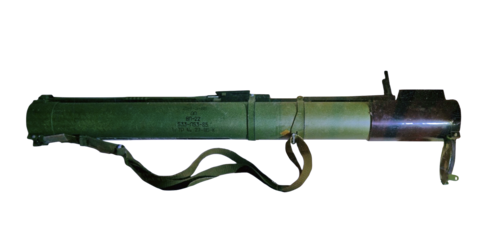
\includegraphics{../images/rpg_wyrzutnie/rpg-22_1.jpg}
\caption{RPG-22 Netto --- jednorazowy granatnik}
\end{figure}

\subsection{Opis}\label{opis-85}

RPG-22 Netto (Нетто) to radziecki jednorazowy granatnik rakietowy
kalibru 72,5 mm opracowany przez GSKB-47 i przyjęty do służby w 1980
roku jako modernizacja RPG-18. Powiększony kaliber (72,5 mm vs 64 mm
RPG-18) i ulepszona głowica kumulacyjna dają przenikanie do 400 mm
pancerza --- dwa razy więcej niż RPG-18. RPG-22 jest ulepszoną wersją
koncepcji ``jednorazówki dla każdego żołnierza'' --- prosta, lekka (2,7
kg), niezawodna. Stosowany przez armie byłego ZSRR; wycofywany przez
RPG-26 i RPG-27, ale wciąż spotykany w magazynach i na polach walki.

\subsection{Dane techniczne}\label{dane-techniczne-85}

\begin{longtable}[]{@{}ll@{}}
\toprule\noalign{}
Parametr & Wartość \\
\midrule\noalign{}
\endhead
\bottomrule\noalign{}
\endlastfoot
Typ & Jednorazowy granatnik rakietowy \\
Kraj produkcji & ZSRR / Rosja \\
Rok wprowadzenia & 1980 \\
Kaliber & 72,5 mm \\
Długość (złożony) & 755 mm \\
Długość (rozłożony do strzału) & 1 060 mm \\
Masa & 2,7 kg \\
Przenikanie pancerza & 400 mm \\
Zasięg skuteczny & 250 m \\
Obsługa & 1 osoba \\
\end{longtable}

\subsection{Charakterystyczne cechy
rozpoznawcze}\label{charakterystyczne-cechy-rozpoznawcze-85}

\begin{quote}
Jak odróżnić RPG-22 od RPG-18 i RPG-26:
\end{quote}

\begin{itemize}
\tightlist
\item
  \textbf{Grubsza rura 72,5 mm --- cieńsza od RPG-26 (72,5 mm podobny),
  grubsza od RPG-18 (64 mm):} RPG-22 i RPG-26 mają ten sam kaliber 72,5
  mm --- trudne do odróżnienia po grubości rury; główna różnica to
  oznaczenia i wygląd osłony celownika
\item
  \textbf{Teleskopowa rura --- rozsuwana do strzału:} RPG-22 (jak
  RPG-18) ma teleskopową tubę, którą rozsuwamy przed strzałem; RPG-26
  jest nierozsuwany --- rura jest stała; ta różnica w mechanizmie
  rozłożenia jest kluczowa
\item
  \textbf{Mniejszy i prostszy celownik niż RPG-26:} RPG-22 ma
  prosto­kątny wizjer celowniczy mniejszy niż RPG-26; wygląd celownika
  jest ``starszy'' i prostszy
\item
  \textbf{Wyraźnie prostszy mechanizm obsługi niż RPG-26:} RPG-22 wymaga
  ręcznego rozsunięcia tuby i odchylenia celownika; RPG-26 ma
  nowocześniejszy mechanizm uzbrojenia; przy obserwacji obsługi różnica
  jest widoczna
\item
  \textbf{Jeden z najlżejszych jednorazowych granatników --- 2,7 kg:}
  RPG-22 waży 2,7 kg --- prawie tak samo jak RPG-18 (2,6 kg) i RPG-26
  (2,9 kg); ta lekkość jest wspólna dla całej rodziny ``lekkich
  jednorazówek''
\item
  \textbf{Stary wygląd --- archaiczna konstrukcja z lat 80.:} RPG-22
  jest wizualnie starszy od RPG-26 i nowszych; prostsze elementy, mniej
  ergonomiczne uchwyty; ``retro'' wśród jednorazowych granatników
\end{itemize}

\subsection{Ciekawostka}\label{ciekawostka-85}

\begin{quote}
RPG-22 pojawił się w Afganistanie w 1981 roku i był pierwszą radziecką
jednorazówką szeroko stosowaną w konflikcie. Sowieci dostarczali
żołnierzom RPG-22 jako uzupełnienie RPG-7 --- pierwszy raz żołnierze
mogli nosić ``zapas'' rakiet w formie lekkich jednorazówek. Mudżahedini
szybko nauczyli się ich używać ze zdobytych egzemplarzy. Paradoksalnie,
``jednorazowa rura dla mas'' stała się pożądanym łupem, bo był znacznie
prostszy w obsłudze niż RPG-7 dla nieszkołonego bojownika.
\end{quote}

\section{Jednorazowy granatnik RPG-26
Agleń}\label{jednorazowy-granatnik-rpg-26-agleux144}

\subsubsection{RPG-26 Aglen Disposable Rocket Launcher \textbar{} РПГ-26
«Аглень»}\label{rpg-26-aglen-disposable-rocket-launcher-ux440ux43fux433-26-ux430ux433ux43bux435ux43dux44c}

\begin{center}\rule{0.5\linewidth}{0.5pt}\end{center}

\begin{figure}
\centering
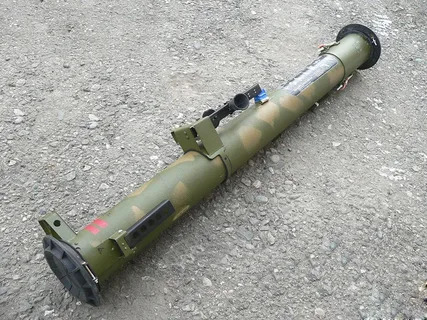
\includegraphics{../images/rpg_wyrzutnie/rpg-26_1.jpg}
\caption{RPG-26 Agleń --- jednorazowy granatnik}
\end{figure}

\subsection{Opis}\label{opis-86}

RPG-26 Agleń (Аглень --- dawna nazwa miejscowości) to radziecki
jednorazowy granatnik rakietowy kalibru 72,5 mm opracowany przez GSKB-47
i przyjęty do służby w 1985 roku jako bezpośredni następnik RPG-22.
Ulepszona głowica kumulacyjna przebija do 440 mm pancerza jednolitego
--- znacznie więcej niż RPG-18 (200 mm) i RPG-22 (400 mm). RPG-26 jest
standardową ``jednorazówką'' rosyjskiej piechoty --- prosta, lekka (2,9
kg), niezawodna. Wystarczy do rażenia starszych czołgów od boku i tyłu
(bez ERA), BWP, APC, MRAP i umocnień polowych. Wycofywany przez RPG-27,
RPG-30 i bardziej zaawansowane systemy, ale wciąż powszechny w
rosyjskich magazynach i na polach walki.

\subsection{Dane techniczne}\label{dane-techniczne-86}

\begin{longtable}[]{@{}ll@{}}
\toprule\noalign{}
Parametr & Wartość \\
\midrule\noalign{}
\endhead
\bottomrule\noalign{}
\endlastfoot
Typ & Jednorazowy granatnik rakietowy \\
Kraj produkcji & ZSRR / Rosja \\
Rok wprowadzenia & 1985 \\
Kaliber & 72,5 mm \\
Długość (złożony) & 770 mm \\
Długość (rozłożony do strzału) & 1 020 mm \\
Masa & 2,9 kg \\
Przenikanie pancerza & 440 mm \\
Zasięg skuteczny & 250 m \\
Obsługa & 1 osoba \\
\end{longtable}

\subsection{Charakterystyczne cechy
rozpoznawcze}\label{charakterystyczne-cechy-rozpoznawcze-86}

\begin{quote}
Jak odróżnić RPG-26 od RPG-18 i RPG-22:
\end{quote}

\begin{itemize}
\tightlist
\item
  \textbf{Grubsza rura 72,5 mm --- wyraźnie szersza niż RPG-18 (64 mm):}
  RPG-26 jest grubszy od RPG-18; przy bezpośrednim porównaniu różnica
  kalibrów 64 vs 72,5 mm jest wyczuwalna; RPG-26 i RPG-22 mają podobny
  kaliber, więc tutaj różnica jest mniejsza
\item
  \textbf{Charakterystyczny mały wizjer z przeziernikiem --- bardziej
  rozbudowany niż RPG-18:} RPG-26 ma prostokątny wizjer celowniczy z
  oznaczeniami odległości; bardziej rozbudowany niż prosty wizjer
  RPG-18; mniej rozbudowany niż celownik RPG-7
\item
  \textbf{Ograniczona liczba zewnętrznych elementów --- ``czysta'' rura
  z osłoną:} RPG-26 ma minimalne elementy zewnętrzne --- głównie
  cylindryczna rura z osłoną uchwytu i celownikiem; prostszy wizualnie
  niż RPG-27 czy RPG-29
\item
  \textbf{Prosty mechanizm uzbrojenia przez wysunięcie tylnej pokrywy:}
  RPG-26 uzbraja się przez wysunięcie tylnej osłony (tzw. ``stożka
  odgazowania'') ku tyłowi; ten prosty ruch odbezpiecza broń; każda
  jednorazówka ma inny mechanizm, ale RPG-26 jest szczególnie prosty
\item
  \textbf{Jednorazowy --- wyrzucany po strzale:} jak wszystkie
  jednorazowe; porzucone tubusy RPG-26 na polu walki mają
  charakterystyczny wypalony wylot i metalową osłonę
\item
  \textbf{Brak stożkowej tylnicy RPG-7:} w odróżnieniu od RPG-7 (z
  rozszerzonym stożkiem z tyłu) RPG-26 ma prostą cylindryczną rurę bez
  rozszerzenia; to kluczowa różnica wizualna między jednorazowym a
  wielokrotnego użytku
\end{itemize}

\subsection{Ciekawostka}\label{ciekawostka-86}

\begin{quote}
RPG-26 w wojnie na Ukrainie stał się jedną z najczęstszych
``porzuconych'' broni znajdowanych przez obie strony. Prostota obsługi
(jedna osoba, nie wymaga szkolenia poza podstawowym) i niska cena
sprawiają, że rosyjska piechota nosiła RPG-26 jako standardowe
wyposażenie indywidualne. Na filmach z ukraińskich pól walki widać
często porzucone niestrzelone lub strzelone tubusy RPG-26, RPG-18 i
RPG-22 --- co daje obraz, jak powszechna jest jednorazowa broń rakietowa
w nowoczesnej wojnie piechoty.
\end{quote}

\section{Jednorazowy granatnik RPG-27
Tavolga}\label{jednorazowy-granatnik-rpg-27-tavolga}

\subsubsection{RPG-27 Tavolga Disposable Rocket Launcher \textbar{}
РПГ-27
«Таволга»}\label{rpg-27-tavolga-disposable-rocket-launcher-ux440ux43fux433-27-ux442ux430ux432ux43eux43bux433ux430}

\begin{center}\rule{0.5\linewidth}{0.5pt}\end{center}

\begin{figure}
\centering
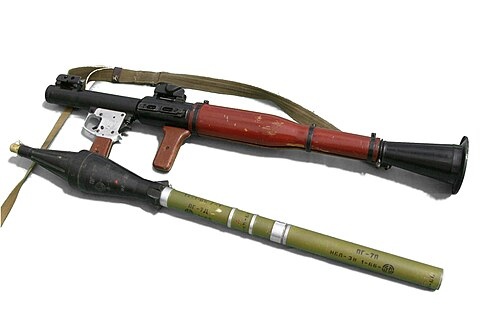
\includegraphics{../images/rpg_wyrzutnie/rpg-27_1.jpg}
\caption{RPG-27 Tavolga --- ciężki granatnik}
\end{figure}

\subsection{Opis}\label{opis-87}

RPG-27 Tavolga (Таволга --- Tawuła, rodzaj rośliny) to rosyjski
jednorazowy granatnik przeciwpancerny kalibru 105 mm opracowany przez
GNPP Bazalt i przyjęty do służby w 1990 roku jako ciężka jednorazówka
dla piechoty. Używa tej samej głowicy tandemowej co wielokrotnego użytku
RPG-29 (PG-29V) --- co daje przenikanie ponad 750 mm pancerza za ERA.
Łączy zatem ogromną siłę penetracji z prostotą jednorazowej broni. Masa
8 kg i kaliber 105 mm czynią go ciężkim jak na jednorazówkę, ale głowica
tandemowa umożliwia niszczenie nowoczesnych czołgów --- czego RPG-18, 22
i 26 nie potrafią. Stosowany przez rosyjskie siły specjalne i piechotę
szturmową.

\subsection{Dane techniczne}\label{dane-techniczne-87}

\begin{longtable}[]{@{}ll@{}}
\toprule\noalign{}
Parametr & Wartość \\
\midrule\noalign{}
\endhead
\bottomrule\noalign{}
\endlastfoot
Typ & Ciężki jednorazowy granatnik rakietowy \\
Kraj produkcji & Rosja \\
Rok wprowadzenia & 1990 \\
Kaliber & 105 mm \\
Długość & 1 155 mm \\
Masa & 8,0 kg \\
Przenikanie pancerza & \textgreater750 mm za ERA (tandem) \\
Zasięg skuteczny & 200 m \\
Obsługa & 1 osoba \\
\end{longtable}

\subsection{Charakterystyczne cechy
rozpoznawcze}\label{charakterystyczne-cechy-rozpoznawcze-87}

\begin{quote}
Jak odróżnić RPG-27 od RPG-26 i RPG-29:
\end{quote}

\begin{itemize}
\tightlist
\item
  \textbf{Gruba rura 105 mm, jednorazowa --- grubsza niż RPG-26 (72,5
  mm):} RPG-27 ma wyraźnie grubszą tubę niż lekkie jednorazówki; kaliber
  105 mm to prawie połowa grubości więcej niż 72,5 mm; przy bezpośrednim
  porównaniu bardzo wyraźna różnica
\item
  \textbf{Jednorazowy --- brak składanej lufy (w odróżnieniu od
  RPG-29):} RPG-27 (jednorazowy) ma jedną stałą tubę; RPG-29
  (wielokrotnego użytku) jest składany w dwóch sekcjach; to klucz do
  odróżnienia obu systemów 105 mm
\item
  \textbf{Cięższy i dłuższy od RPG-26 --- 8 kg vs 2,9 kg:} RPG-27 jest
  wyraźnie cięższy; strzelec noszący RPG-27 niesie wyraźnie ciężką broń;
  przy transporcie widać ciężar i rozmiar; RPG-26 jest ``prawie lekki''
  w porównaniu
\item
  \textbf{Tandemowa głowica --- dwa złączone stożki ``nosa'' pocisku:}
  pocisk PG-27 (tandemowy) ma charakterystyczny ``dwustożkowy'' nos z
  mniejszą głowicą wstępną i większą główną; inny kształt niż proste
  głowice RPG-18/26
\item
  \textbf{Brak małej rury pobocznej RPG-30:} RPG-30 ma dwie równoległe
  rury; RPG-27 ma tylko jedną grubą rurę; ta różnica natychmiast
  odróżnia RPG-27 od RPG-30
\item
  \textbf{Mały wizjer celowniczy bez optyki --- prosty przyrząd:} RPG-27
  ma prosty mechaniczny celownik; wygląd jest ``jednorazowy'' --- bez
  zaawansowanej optyki ani elektroniki
\end{itemize}

\subsection{Ciekawostka}\label{ciekawostka-87}

\begin{quote}
RPG-27 był jedną z pierwszych broni jednorazowych zdolnych do pokonania
pancerza reaktywnego ERA --- co w 1990 roku było rewolucją. Dotychczas
jednorazowe granatniki (RPG-18, 22, 26) były nieskuteczne przeciwko
czołgom z ERA; żołnierz musiał używać wielokrotnego użytku RPG-7 z
głowicą tandemową. RPG-27 połączył prostotę jednorazówki z mocą głowicy
tandemowej --- ale ceną była masa 8 kg, co dla jednorazowej broni jest
dużo. Żołnierze rosyjscy w Afganistanie i Czeczenii nosili go tylko na
specjalne zadania ``zneutralizowania czołgu'' --- nie jako standardową
broń indywidualną.
\end{quote}

\section{Granatnik przeciwpancerny RPG-29
Wampir}\label{granatnik-przeciwpancerny-rpg-29-wampir}

\subsubsection{RPG-29 Vampir Anti-Tank Grenade Launcher \textbar{}
РПГ-29
«Вампир»}\label{rpg-29-vampir-anti-tank-grenade-launcher-ux440ux43fux433-29-ux432ux430ux43cux43fux438ux440}

\begin{center}\rule{0.5\linewidth}{0.5pt}\end{center}

\begin{figure}
\centering
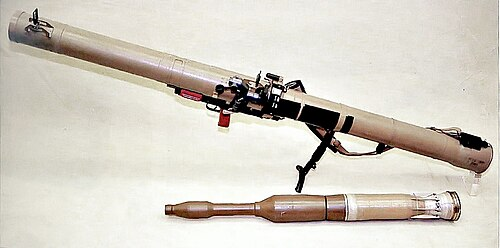
\includegraphics{../images/rpg_wyrzutnie/rpg-29_1.jpg}
\caption{RPG-29 Wampir --- granatnik przeciwpancerny}
\end{figure}

\subsection{Opis}\label{opis-88}

RPG-29 Wampir (Вампир --- Wampir) to rosyjski granatnik przeciwpancerny
wielokrotnego użytku kalibru 105 mm opracowany przez GSKB-47 i przyjęty
do służby w 1989 roku. Wyróżnia się potężną głowicą tandemową PG-29V
przebijającą ponad 750 mm pancerza za ERA --- co pozwala na niszczenie
czołgów T-72 z pancerzem reaktywnym, T-90 i potencjalnie M1A2 Abrams od
strony bocznej. Jest to jeden z najpotężniejszych przenośnych
granatników przeciwpancernych na świecie. RPG-29 jest składany --- lufa
i komora rozkładają się, co ułatwia transport. Stosowany przez rosyjskie
siły specjalne i wybranych jednostki; eksportowany do Syrii, Iranu i
Hezbollahu; używany przez Hezbollah do trafienia izraelskich Merkav w
2006 roku.

\subsection{Dane techniczne}\label{dane-techniczne-88}

\begin{longtable}[]{@{}ll@{}}
\toprule\noalign{}
Parametr & Wartość \\
\midrule\noalign{}
\endhead
\bottomrule\noalign{}
\endlastfoot
Typ & Granatnik przeciwpancerny wielokrotnego użytku \\
Kraj produkcji & Rosja \\
Rok wprowadzenia & 1989 \\
Kaliber & 105 mm \\
Długość (złożony) & 1 000 mm \\
Długość (do strzału) & 1 850 mm \\
Masa (bez pocisku) & 11,5 kg \\
Przenikanie pancerza & \textgreater750 mm za ERA (tandem PG-29V) \\
Zasięg skuteczny & 500 m \\
Obsługa & 2 osoby \\
\end{longtable}

\subsection{Charakterystyczne cechy
rozpoznawcze}\label{charakterystyczne-cechy-rozpoznawcze-88}

\begin{quote}
Jak odróżnić RPG-29 od RPG-7 i RPG-27:
\end{quote}

\begin{itemize}
\tightlist
\item
  \textbf{Składana lufa w dwóch sekcjach --- rozkładana do strzału:}
  RPG-29 ma lufę składaną w połowie --- dwie sekcje łączone przed
  strzałem; to kluczowa cecha wizualna; RPG-7 ma jednoczęściową lufę;
  widok składania RPG-29 jest charakterystyczny
\item
  \textbf{Ogromny kaliber 105 mm --- wyraźnie grubsza rura niż RPG-7:}
  RPG-29 ma kaliber 105 mm vs 40 mm lufy RPG-7; rura RPG-29 jest
  znacznie grubsza; pocisk PG-29V o kalibrze 105 mm jest ogromny i
  wyraźnie grubszy niż pociski RPG-7
\item
  \textbf{Masywny, ciężki zestaw --- 11,5 kg bez pocisku:} RPG-29 jest
  wyraźnie cięższy od RPG-7 (6,3 kg); przy przenoszeniu widać, że to
  ciężka broń wymagająca dwóch ludzi do sprawnej obsługi
\item
  \textbf{Charakterystyczny tandemowy pocisk PG-29V:} głowica PG-29V ma
  widoczną tandemową konstrukcję --- mniejsza głowica wstępna z przodu,
  większa główna za nią; ten ``dwuczłonowy'' wygląd pocisku odróżnia go
  od prostszych głowic RPG-7
\item
  \textbf{Celownik optyczny z bocznym montażem jak w RPG-7:} RPG-29 ma
  celownik optyczny po lewej stronie komory --- podobnie jak RPG-7; ale
  całość jest wyraźnie masywniejsza i nowocześniejsza
\item
  \textbf{Dwie osoby do obsługi i transportu:} obsługa RPG-29 wymaga
  dwóch ludzi (strzelec + ładowniczy); jednorazowe (RPG-18, 22, 26)
  obsługuje 1 osoba; RPG-7 może obsługiwać 1 osoba, ale zwykle jest
  asystent; RPG-29 zawsze wymaga pary
\end{itemize}

\subsection{Ciekawostka}\label{ciekawostka-88}

\begin{quote}
W 2006 roku podczas drugiej wojny libańskiej Hezbollah użył RPG-29 do
trafienia izraelskich czołgów Merkava IV --- uważanych za najlepiej
chronione czołgi na świecie. Trafienie od strony bocznej lub tylnej
spowodowało przebicie pancerza reaktywnego i uszkodzenie wnętrza. Armia
izraelska była zszokowana --- i natychmiast wszczęła dochodzenie, jak
broń tak nowa i rzadka trafiła do Hezbollahu. Ustalono, że Syria i Iran
przekazały RPG-29 jako ``prezent'' dla Hezbollahu. Incydent spowodował
modyfikację taktyki izraelskich czołgów i przyspieszył instalację
systemów aktywnej ochrony Trophy.
\end{quote}

\section{Granatnik przeciwpancerny RPG-30
Kryuk}\label{granatnik-przeciwpancerny-rpg-30-kryuk}

\subsubsection{RPG-30 Kryuk Anti-Tank Grenade Launcher \textbar{} РПГ-30
«Крюк»}\label{rpg-30-kryuk-anti-tank-grenade-launcher-ux440ux43fux433-30-ux43aux440ux44eux43a}

\begin{center}\rule{0.5\linewidth}{0.5pt}\end{center}

\begin{figure}
\centering
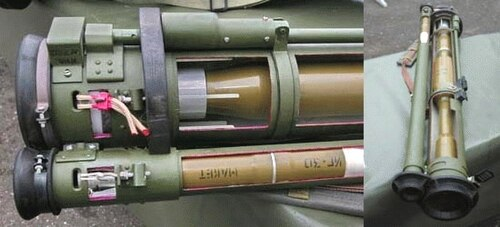
\includegraphics{../images/rpg_wyrzutnie/rpg-30_1.jpg}
\caption{RPG-30 Kryuk --- granatnik z systemem APS}
\end{figure}

\subsection{Opis}\label{opis-89}

RPG-30 Kryuk (Крюк --- Hak) to rosyjski jednorazowy granatnik
przeciwpancerny kalibru 105 mm opracowany przez GNPP Bazalt i przyjęty
do służby w 2008 roku. Wyróżnia się unikalnym systemem ``fałszywego
pocisku'' --- przed głowicą główną wystrzeliwana jest mała
rakieta-przynęta (kaliber 40 mm), która wyzwala systemy aktywnej ochrony
czołgu (jak Shtora, Arena, Trophy); po ułamku sekundy główna głowica 105
mm trafia w cel pozbawiony już obrony aktywnej. RPG-30 jest jedyną na
świecie masową bronią jednorazową zaprojektowaną specjalnie do
pokonywania systemów aktywnej ochrony czołgów. Niezwykle nowoczesna
koncepcja w jednorazowym, lekkim granatniki.

\subsection{Dane techniczne}\label{dane-techniczne-89}

\begin{longtable}[]{@{}ll@{}}
\toprule\noalign{}
Parametr & Wartość \\
\midrule\noalign{}
\endhead
\bottomrule\noalign{}
\endlastfoot
Typ & Jednorazowy granatnik z systemem neutralizacji APS \\
Kraj produkcji & Rosja \\
Rok wprowadzenia & 2008 \\
Kaliber główny & 105 mm \\
Kaliber przynęty & 40 mm \\
Długość & 1 135 mm \\
Masa & 10,3 kg \\
Przenikanie pancerza & \textgreater650 mm za ERA \\
Zasięg skuteczny & 200 m \\
Obsługa & 1 osoba \\
\end{longtable}

\subsection{Charakterystyczne cechy
rozpoznawcze}\label{charakterystyczne-cechy-rozpoznawcze-89}

\begin{quote}
Jak odróżnić RPG-30 od RPG-26, RPG-27 i RPG-29:
\end{quote}

\begin{itemize}
\tightlist
\item
  \textbf{Dwie równoległe rury --- duża i mała obok siebie:} RPG-30 ma
  charakterystyczny wygląd z DWOMA równoległymi tubusami --- grubą tubą
  105 mm z głównym pociskiem i cienką tubą 40 mm z pociskiem-przynętą;
  żaden inny granatnik nie ma dwóch równoległych rur; to natychmiastowy
  identyfikator RPG-30
\item
  \textbf{Cienka dodatkowa rura po boku głównej --- ``przyczepka'':}
  mała tuba 40 mm jest przymocowana z boku grubej tuby 105 mm; ten
  ``przyczepiony'' mały cylinder jest unikalny wizualnie i natychmiast
  zwraca uwagę
\item
  \textbf{Jednorazowy --- wyrzucany po strzale (ale ciężki):} RPG-30
  waży 10,3 kg --- to ciężka jednorazówka; lżejsze jednorazowe (RPG-26
  --- 2,9 kg, RPG-18 --- 2,6 kg) są wyraźnie mniejsze i lżejsze
\item
  \textbf{Brak składania lufy (w odróżnieniu od RPG-29):} RPG-30 jest
  jednorazowy i nie składa lufy; RPG-29 (wielokrotnego użytku) ma
  składaną lufę w dwóch sekcjach --- ta różnica pomaga odróżnić oba
  systemy kalibrów 105 mm
\item
  \textbf{Bardzo rzadki na polach walki --- broń specjalistyczna:}
  RPG-30 jest kosztowny i produkowany w ograniczonych ilościach; widok
  tej broni sugeruje wyspecjalizowaną jednostkę lub szczególnie
  wyposażoną piechotę; w masowej piechoty nie jest powszechny
\item
  \textbf{Nowoczesne, obłe kształty obudowy --- ``taktyczny'' wygląd:}
  RPG-30 ma nowocześniejszy, bardziej ``taktyczny'' wygląd niż RPG-26
  (prosta rura); obudowa jest bardziej obła i zaawansowana ergonomicznie
\end{itemize}

\subsection{Ciekawostka}\label{ciekawostka-89}

\begin{quote}
RPG-30 jest odpowiedzią na systemy aktywnej ochrony czołgów takie jak
izraelski Trophy (Rafael) i rosyjski Arena. Projektanci Bazalt wpadli na
genialnie prostą koncepcję: zamiast budować szybszy pocisk (trudne i
drogie), wystrzel imitację (prosta i tania), aby ``zużyć'' system
ochrony zanim trafi główna głowica. Systemy Trophy i Arena potrzebują
kilku sekund na przeładowanie po neutralizacji zagrożenia --- a RPG-30
nie daje im tej chwili. Zachodnie armie, kupując systemy aktywnej
ochrony, musiały od razu brać pod uwagę właśnie RPG-30 jako zagrożenie,
które może je ominąć.
\end{quote}

\section{Granatnik wielokrotnego użytku RPG-32
Hashim}\label{granatnik-wielokrotnego-uux17cytku-rpg-32-hashim}

\subsubsection{RPG-32 Hashim Multi-Shot Rocket Launcher \textbar{}
РПГ-32
«Хашим»}\label{rpg-32-hashim-multi-shot-rocket-launcher-ux440ux43fux433-32-ux445ux430ux448ux438ux43c}

\begin{center}\rule{0.5\linewidth}{0.5pt}\end{center}

\begin{figure}
\centering
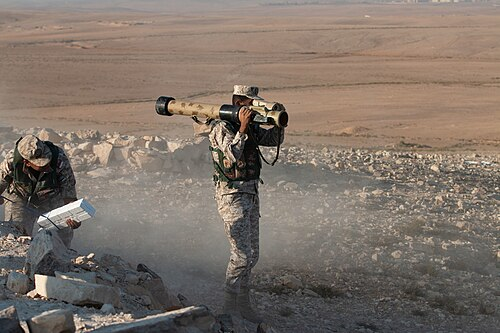
\includegraphics{../images/rpg_wyrzutnie/rpg-32_1.jpg}
\caption{RPG-32 Hashim --- modułowy granatnik}
\end{figure}

\subsection{Opis}\label{opis-90}

RPG-32 Hashim (Хашим --- arabskie imię) to rosyjsko-jordański modułowy
granatnik przeciwpancerny opracowany wspólnie przez GNPP Bazalt (Rosja)
i Jordan Armed Forces (Jordania) i przyjęty do służby w 2014 roku.
Wyróżnia się modułowym systemem ładowania --- do tej samej tuby
wielokrotnego użytku można mocować różne kalibrowe głowice: 72,5 mm
(przeciwpancerne i termobaryczne) oraz 105 mm (tandemowe). RPG-32 jest
produkowany w Jordanii przez Jadara Weaponry w ramach umowy licencyjnej
z Rosją --- jest to rzadki przypadek wspólnej produkcji z arabskim
krajem. Może być używany zarówno przez operatorów w kamizelce z
pojemnikiem głowicy, jak i z wyrzutni montowanej na pojeździe.

\subsection{Dane techniczne}\label{dane-techniczne-90}

\begin{longtable}[]{@{}ll@{}}
\toprule\noalign{}
Parametr & Wartość \\
\midrule\noalign{}
\endhead
\bottomrule\noalign{}
\endlastfoot
Typ & Modułowy wielokrotnego użytku granatnik \\
Kraj produkcji & Rosja / Jordania \\
Rok wprowadzenia & 2014 \\
Kalibry głowic & 72,5 mm / 105 mm \\
Długość (tuba bez głowicy) & 900 mm \\
Masa (tuba) & 3,0 kg \\
Masa (z głowicą 105 mm) & ok. 10 kg \\
Przenikanie pancerza & \textgreater650 mm za ERA (105 mm tandem) \\
Zasięg skuteczny & 200--700 m (zależnie od głowicy) \\
Obsługa & 1--2 osoby \\
\end{longtable}

\subsection{Charakterystyczne cechy
rozpoznawcze}\label{charakterystyczne-cechy-rozpoznawcze-90}

\begin{quote}
Jak odróżnić RPG-32 od RPG-7 i RPG-29:
\end{quote}

\begin{itemize}
\tightlist
\item
  \textbf{Modułowa tuba bez własnej głowicy --- wymienny ``pojemnik'':}
  RPG-32 składa się z oddzielnej tuby (wyrzutni) i oddzielnych
  ``kontenerów z głowicami''; strzelec najpierw ma samą tubę, potem
  przykłada głowicę; ten modułowy układ jest wizualnie unikalny ---
  zobaczyć strzelca noszącego oddzielnie tubę i oddzielnie zasobniki
  głowic
\item
  \textbf{Charakterystyczna tuba wielokrotnego użytku --- bez
  rozszerzenia tylnego:} RPG-32 ma prostą tubę bez charakterystycznego
  stożkowego rozszerzenia RPG-7; proporcje są bardziej ``nowoczesne'' i
  cylindryczne
\item
  \textbf{Głowice 72,5 mm i 105 mm wyglądają inaczej od siebie:} przy
  montowaniu głowicy 72,5 mm na tubę efekt jest ``mniejsza głowica na
  dużej tubie''; przy 105 mm --- ``duża głowica na tubie''; ta zmienność
  rozmiarów jest charakterystyczna
\item
  \textbf{Rzadkość poza Jordanią i krajami arabskimi:} RPG-32 jest
  eksportowany głównie przez Jordanię do krajów arabskich; w rosyjskiej
  armii jest mało powszechny; widok tej broni sugeruje jordańskie wojsko
  lub eksport na Bliski Wschód
\item
  \textbf{Nowoczesny celownik z dodatkowym montażem optyki:} RPG-32 ma
  nowoczesny modułowy celownik z możliwością montażu celownika
  noktowizyjnego; bardziej zaawansowany wizualnie niż klasyczny celownik
  RPG-7
\item
  \textbf{Tuba lżejsza od RPG-7 --- 3 kg vs 6,3 kg:} tuba RPG-32 bez
  głowicy waży tylko 3 kg; strzelec nosi ją lekko; dopiero po dołączeniu
  głowicy masa rośnie do 10 kg; ta różnica w transporcie jest widoczna
\end{itemize}

\subsection{Ciekawostka}\label{ciekawostka-90}

\begin{quote}
RPG-32 jest pierwszą rosyjską bronią wyprodukowaną oficjalnie za granicą
przez niebędące byłym ZSRR państwo --- Jordanię. Umowa licencyjna z 2010
roku była częścią rosyjskiej strategii penetracji rynku
bliskowschodniego przez wspólne projekty obronne. Jordania ---
tradycyjnie proamerykanin --- zdecydowała się na rosyjski RPG-32 zamiast
zachodnich odpowiedników z przyczyn czysto pragmatycznych: był tańszy,
prostszy w obsłudze i produkowany lokalnie. Dla Rosji to sukces
marketingowy: ``wykonany w Jordanii'' brzmi neutralnie, a wpływ
rosyjskiej technologii jest oczywisty dla każdego znającego temat.
\end{quote}

\section{Jednorazowy granatnik termobaryczny
RShG-1}\label{jednorazowy-granatnik-termobaryczny-rshg-1}

\subsubsection{RShG-1 Thermobaric Rocket Launcher \textbar{}
РШГ-1}\label{rshg-1-thermobaric-rocket-launcher-ux440ux448ux433-1}

\begin{center}\rule{0.5\linewidth}{0.5pt}\end{center}

\begin{figure}
\centering
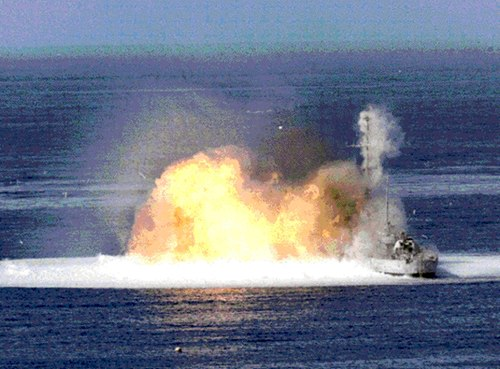
\includegraphics{../images/rpg_wyrzutnie/rshg-1_1.jpg}
\caption{RShG-1 --- granatnik termobaryczny}
\end{figure}

\subsection{Opis}\label{opis-91}

RShG-1 (Реактивная Штурмовая Граната --- Reaktywny szturmowy granat) to
rosyjski jednorazowy granatnik z głowicą termobaryczną kalibru 105 mm
opracowany przez GNPP Bazalt i przyjęty do służby w 1999 roku. Nie jest
bronią przeciwpancerną --- jego głowica termobaryczna (fuel-air
explosive, FAE) niszczy siłę żywą w schronach, bunkrach, budynkach i na
otwartym terenie przez falę ciśnienia i wypalenie tlenu w zamkniętych
przestrzeniach. Jeden strzał RShG-1 niszczy wszystkie żywe istoty w
schronie o objętości do 100 m³ lub na otwartym terenie w promieniu 10 m.
Stosowany masowo w Czeczenii i Syrii do ``oczyszczania'' budynków i
podziemi.

\subsection{Dane techniczne}\label{dane-techniczne-91}

\begin{longtable}[]{@{}ll@{}}
\toprule\noalign{}
Parametr & Wartość \\
\midrule\noalign{}
\endhead
\bottomrule\noalign{}
\endlastfoot
Typ & Jednorazowy granatnik termobaryczny \\
Kraj produkcji & Rosja \\
Rok wprowadzenia & 1999 \\
Kaliber & 105 mm \\
Długość & 1 100 mm \\
Masa & 8,8 kg \\
Rodzaj głowicy & Termobaryczna (FAE) \\
Zasięg skuteczny & 200 m \\
Obsługa & 1--2 osoby \\
\end{longtable}

\subsection{Charakterystyczne cechy
rozpoznawcze}\label{charakterystyczne-cechy-rozpoznawcze-91}

\begin{quote}
Jak odróżnić RShG-1 od RPG-27 i RPG-7 z głowicą TBG:
\end{quote}

\begin{itemize}
\tightlist
\item
  \textbf{Identyczne zewnętrznie z RPG-27 --- różnica tylko w głowicy:}
  RShG-1 i RPG-27 mają bardzo podobne rozmiary i kształt tuby; główna
  różnica to kształt głowicy --- RShG-1 ma charakterystyczną ``tępą''
  głowicę termobaryczną (bez piezoelektrycznego igłowego nosa jak HEAT);
  ten ``tępy nos'' głowicy jest kluczowym wyróżnikiem wizualnym
\item
  \textbf{Tępa, cylindryczna głowica bez piezoelektrycznego nosa:}
  głowice HEAT mają charakterystyczny długi ``iglicowy'' nos
  piezoelektryczny; głowice termobaryczne mają krótszy, bardziej
  zaokrąglony lub ``tępy'' nos; ta różnica kształtu głowicy pozwala
  odróżnić RShG-1 od RPG-27
\item
  \textbf{Żółte lub pomarańczowe oznaczenia na głowicy i tubie:} głowice
  termobaryczne mają zwyczajowo żółte (lub pomarańczowe) oznaczenia
  kolorem --- standard rosyjski dla broni termobarycznej; HEAT ma
  czerwone lub beżowe oznaczenia; kolor etykiet jest sygnałem
\item
  \textbf{Brak właściwości przeciwpancernych --- inne zastosowanie
  taktyczne:} RShG-1 nie jest używany do strzelania do czołgów; widok
  żołnierza używającego go przy szturmie budynku (nie przy pojeździe)
  sugeruje termobaryczny charakter
\item
  \textbf{Masa 8,8 kg --- porównywalna z RPG-27 (8 kg):} podobna masa do
  RPG-27; wyraźnie cięższy od jednorazówek 72,5 mm (RPG-26 --- 2,9 kg);
  ta masa jest charakterystyczna dla ``ciężkich jednorazówek 105 mm''
\item
  \textbf{Wersja lżejsza --- RShG-2 (72,5 mm):} istnieje też lżejsza
  wersja RShG-2 kalibru 72,5 mm (\textasciitilde3,8 kg); odróżnienie od
  RShG-1 po kalibrze tuby (cieńsza rura) i mniejszych rozmiarach całości
\end{itemize}

\subsection{Ciekawostka}\label{ciekawostka-91}

\begin{quote}
RShG-1 był masowo stosowany przez rosyjskie siły w Czeczenii --- podczas
walk w Groznym w 1999--2000 roku żołnierze opisywali go jako ``narzędzie
do oczyszczania piwnic i klatek schodowych''. Jedna głowica
termobaryczna w przestrzeni zamkniętej eliminuje siłę żywą bez
konieczności wejścia do środka i ręcznej walki. Czeczeńscy bojownicy
doświadczyli tego jako szczególnie przerażającej broni --- bo nie było
ochrony przed falą ciśnienia i temperaturą w zamkniętych schronach.
Human Rights Watch udokumentowało użycie RShG-1 w Syrii i Czeczenii,
podnosząc kwestię proporcjonalności w terenach zamieszkanych.
\end{quote}

\section{Wyrzutnia termobaryczna RPO-A
Szmiel}\label{wyrzutnia-termobaryczna-rpo-a-szmiel}

\subsubsection{RPO-A Shmel Thermobaric Launcher \textbar{} РПО-А
«Шмель»}\label{rpo-a-shmel-thermobaric-launcher-ux440ux43fux43e-ux430-ux448ux43cux435ux43bux44c}

\begin{center}\rule{0.5\linewidth}{0.5pt}\end{center}

\begin{figure}
\centering
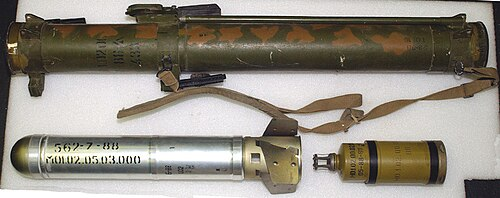
\includegraphics{../images/rpg_wyrzutnie/shmel_1.jpg}
\caption{RPO-A Szmiel --- wyrzutnia termobaryczna}
\end{figure}

\subsection{Opis}\label{opis-92}

RPO-A Szmiel (Шмель --- Trzmiel) to radziecko-rosyjski jednorazowy
granatnik termobaryczny kalibru 93 mm opracowany przez GNPP Bazalt i
przyjęty do służby w 1988 roku. Szmiel nie jest bronią przeciwpancerną
--- to ``ogniotna'' broń piechoty do rażenia celów żywych w budynkach,
schronach, pojazdach opancerzonych (lekkich) i umocnień polowych przez
efekt termobaryczny. Głowica RPO-A detonuje w środku celu, wytwarzając
temperaturę ponad 800°C i falę ciśnienia niszczącą wszystko w promieniu
5 m (schrony zamknięte --- 80 m³). Jest uważany za najskuteczniejszą
przenośną broń termobaryczną na świecie i był masowo stosowany w
Afganistanie, Czeczenii, Syrii i Ukrainie.

\subsection{Dane techniczne}\label{dane-techniczne-92}

\begin{longtable}[]{@{}ll@{}}
\toprule\noalign{}
Parametr & Wartość \\
\midrule\noalign{}
\endhead
\bottomrule\noalign{}
\endlastfoot
Typ & Jednorazowy granatnik termobaryczny \\
Kraj produkcji & ZSRR / Rosja \\
Rok wprowadzenia & 1988 \\
Kaliber & 93 mm \\
Długość & 920 mm \\
Masa & 11,0 kg \\
Rodzaj głowicy & Termobaryczna (FAE) \\
Zasięg skuteczny & 200 m (schrony) / 600 m (tereny otwarte) \\
Obsługa & 1--2 osoby \\
\end{longtable}

\subsection{Charakterystyczne cechy
rozpoznawcze}\label{charakterystyczne-cechy-rozpoznawcze-92}

\begin{quote}
Jak odróżnić RPO-A Szmiel od RShG-1 i lekkich granatników:
\end{quote}

\begin{itemize}
\tightlist
\item
  \textbf{Szarawozielona lub ciemnozielona metalowa tuba --- inny kolor
  niż RPG:} Szmiel ma charakterystyczny metalowy tubę w kolorze
  ciemnozielonym lub oliwkowym --- bardziej ``artyleryjskim'' niż czarne
  lub szare tuby RPG-26/27; ten kolor jest pierwszą wskazówką
\item
  \textbf{Masywna, okrągła tuba bez rozszerzenia tylnego:} Szmiel ma
  prostą, jednoczęściową cylindryczną tubę bez stożkowego rozszerzenia z
  tyłu (charakterystycznego dla RPG-7); proporcje są ``kanciaste'' i
  militarnie proste
\item
  \textbf{Ciężki --- 11 kg --- wyraźnie czuje się ciężar:} Szmiel waży
  11 kg --- to dużo dla jednorazowej broni; strzelec nosi go na ramieniu
  lub trzyma dwoma rękami; wyraźna różnica w ciężarze od lekkich
  jednorazówek (RPG-18 --- 2,6 kg)
\item
  \textbf{Charakterystyczne pomarańczowe lub żółte oznaczenia na tubie:}
  termobaryczne głowice Szmiela mają żółte lub pomarańczowe markings na
  tubie --- standardowe rosyjskie oznaczenia dla broni termobarycznej;
  inne niż oznaczenia broni HEAT
\item
  \textbf{Brak głowicy piezoelektrycznej z nosem ``iglicą'':} Szmiel ma
  zaokrągloną, tępą głowicę bez długiego nosa; w odróżnieniu od HEAT
  RPG-7 widać wyraźnie, że nos jest krótki i zaokrąglony --- ``tuba do
  przenoszenia''
\item
  \textbf{Na ramieniu --- charakterystyczna pozycja strzelecka:} Szmiel
  strzela się z ramienia; charakterystyczna pozycja strzelca z ogromną
  tubą na ramieniu jest podobna do RPG-7, ale Szmiel jest grubszy i
  bardziej ``ciężki'' wizualnie
\end{itemize}

\subsection{Ciekawostka}\label{ciekawostka-92}

\begin{quote}
Szmiel zyskał przydomek ``piechotna artyleria'' w Afganistanie, gdzie
radzieccy żołnierze używali go do ``przepłoszania'' mudżahedinów z
jaskiń i tuneli --- gdzie inaczej musiałaby wejść piechota w
samobójczych szturmach. Jedna głowica Szmiela w tunelu eliminowała
wszystkich wewnątrz bez konieczności kontaktu bezpośredniego. Afgańczycy
bali się Szmiela bardziej niż wielu innych broni rosyjskich --- po jego
użyciu nawet ``bezpieczne'' schrony przestały być bezpieczne. W
Czeczenii Szmiel pojawił się po obu stronach --- część egzemplarzy
zdobyli czeczeńscy bojownicy i używali ich w walkach miejskich w
Groznym.
\end{quote}

\section{Jednorazowy granatnik MRO-A
Bur}\label{jednorazowy-granatnik-mro-a-bur}

\subsubsection{MRO-A Bur Thermobaric Assault Launcher \textbar{} МРО-А
«Бур»}\label{mro-a-bur-thermobaric-assault-launcher-ux43cux440ux43e-ux430-ux431ux443ux440}

\begin{center}\rule{0.5\linewidth}{0.5pt}\end{center}

\begin{figure}
\centering
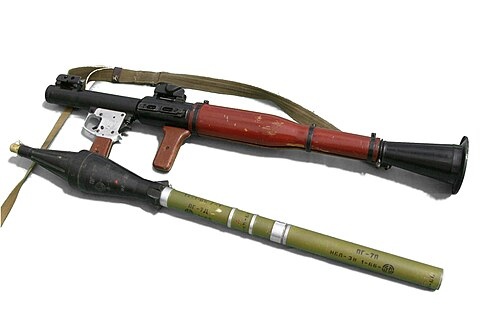
\includegraphics{../images/rpg_wyrzutnie/bur_1.jpg}
\caption{MRO-A Bur --- lekka wyrzutnia termobaryczna}
\end{figure}

\subsection{Opis}\label{opis-93}

MRO-A Bur (Бур --- Wiertło) to rosyjski jednorazowy lekki granatnik
termobaryczny kalibru 72,5 mm opracowany przez GNPP Bazalt jako lżejszy
następnik RPO-A Szmiel, przeznaczony dla żołnierzy piechoty szturmowej i
sił specjalnych. Przyjęty do służby ok. 2014 roku. Waży tylko 4,7 kg (vs
11 kg Szmiela) --- co pozwala żołnierzowi nieść kilka egzemplarzy naraz.
Głowica termobaryczna niszczy cele na otwartym terenie w promieniu 5 m
lub w zamkniętych przestrzeniach do 50--60 m³. Bur może też niszczyć
lekkie pojazdy nieopancerzone i umocnienia polowe. Szeroko stosowany
przez wojska rosyjskie na Ukrainie jako uzupełnienie RPG-7 i cięższych
Szmieli.

\subsection{Dane techniczne}\label{dane-techniczne-93}

\begin{longtable}[]{@{}ll@{}}
\toprule\noalign{}
Parametr & Wartość \\
\midrule\noalign{}
\endhead
\bottomrule\noalign{}
\endlastfoot
Typ & Lekki jednorazowy granatnik termobaryczny \\
Kraj produkcji & Rosja \\
Rok wprowadzenia & ok. 2014 \\
Kaliber & 72,5 mm \\
Długość & 900 mm \\
Masa & 4,7 kg \\
Rodzaj głowicy & Termobaryczna \\
Zasięg skuteczny & 450 m \\
Obsługa & 1 osoba \\
\end{longtable}

\subsection{Charakterystyczne cechy
rozpoznawcze}\label{charakterystyczne-cechy-rozpoznawcze-93}

\begin{quote}
Jak odróżnić MRO-A Bur od RPO-A Szmiel i RPG-26:
\end{quote}

\begin{itemize}
\tightlist
\item
  \textbf{Znacznie lżejszy i cieńszy od Szmiela --- wyraźna różnica
  gabarytów:} Bur waży 4,7 kg vs 11 kg Szmiela i ma kaliber 72,5 mm vs
  93 mm; przy bezpośrednim porównaniu Bur jest wyraźnie cieńszy i
  lżejszy; tuba jest węższa
\item
  \textbf{Podobna masa do RPG-26 (2,9 kg) --- ale nieco cięższy i inny
  kształt głowicy:} Bur jest porównywalny z RPG-26 masą i kalibrem;
  główna różnica to kształt głowicy --- Bur ma tępą głowicę
  termobaryczną; RPG-26 ma iglicowy nos HEAT; kolor oznakowania też się
  różni (żółte vs beżowe)
\item
  \textbf{Tępa głowica bez ``igły'' piezoelektrycznej --- termobaryczny
  charakter:} głowica Bur jest zaokrąglona z przodu bez długiego nosa
  piezoelektrycznego; to odróżnia go od wszystkich granatników HEAT
\item
  \textbf{Żółte lub pomarańczowe markings na tubie --- standard
  termobaryczny:} jak RPO-A i RShG-1, Bur ma żółte lub pomarańczowe
  oznaczenia na tubie informujące o termobarycznym charakterze głowicy
\item
  \textbf{Prosta, jednorodna tuba --- brak teleskopowego rozłożenia:}
  Bur jest stały --- nie rozkłada się jak RPG-18 i RPG-22; prosta
  jednoczęściowa tuba jest gotowa do strzału po odchyleniu celownika
\item
  \textbf{Żołnierz może nieść kilka sztuk --- widoczne ``wiązki''
  Burów:} ze względu na lekkość żołnierze na nagraniach z Ukrainy często
  noszą 2--3 Buri naraz; ta ``wiązka'' lekkich granatników na jednym
  żołnierzu jest charakterystycznym widokiem
\end{itemize}

\subsection{Ciekawostka}\label{ciekawostka-93}

\begin{quote}
Bur stał się ikoną rosyjskiej taktyki piechoty szturmowej na Ukrainie
--- filmiki z żołnierzami szturmującymi budynki z kilkoma Burami naraz
były powszechnie udostępniane na rosyjskich prowojennych kanałach
Telegram. Ukraińscy żołnierze szybko nauczyli się rozpoznawać Bur po
sylwetce i kształcie głowicy --- i zgłaszali, że po ostrzale Burem nawet
żelbetowe pomieszczenia piwniczne stawały się niebezpieczne ze względu
na falę ciśnienia. Bur jest przykładem rosyjskiej filozofii ``lekka i
masowa'' --- zamiast jednego ciężkiego Szmiela, trzech lekkich Burów,
które może nieść jeden żołnierz.
\end{quote}

\section{Nasadkowy granatnik GP-25
Kostior}\label{nasadkowy-granatnik-gp-25-kostior}

\subsubsection{GP-25 Koster Underbarrel Grenade Launcher \textbar{}
ГП-25
«Костёр»}\label{gp-25-koster-underbarrel-grenade-launcher-ux433ux43f-25-ux43aux43eux441ux442ux451ux440}

\begin{center}\rule{0.5\linewidth}{0.5pt}\end{center}

\begin{figure}
\centering
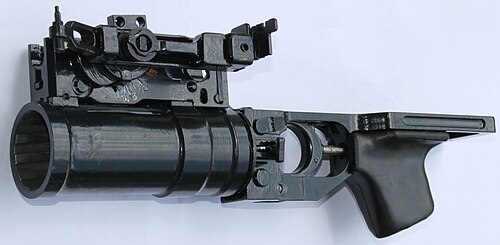
\includegraphics{../images/wyrzutnie_granatow/gp-25_1.jpg}
\caption{GP-25 Kostior --- granatnik podlufowy}
\end{figure}

\subsection{Opis}\label{opis-94}

GP-25 Kostior (Костёр --- Ognisko) to radziecki nasadkowy granatnik
podlufy kalibru 40 mm opracowany przez KBP w Tule i przyjęty do służby w
1978 roku. Montowany pod lufą karabinu szturmowego AK (AKM, AK-74,
AK-74M) bez demontażu broni bazowej --- zamocowany na klamrze pod lufą.
GP-25 pozwala żołnierzowi z karabinem szturmowym na rażenie celów
ukrytych za osłonami (za rogiem, w okopach) na odległość do 400 m
granatami odłamkowymi VOG-25 lub profilaktycznymi (hukowym, dymnym).
Charakterystyczna właściwość: nabój 40×46 mm jest wkładany od przodu
(muzzle-loading), co upraszcza konstrukcję. GP-25 jest standardowym
wyposażeniem wielu armii postsowieckich i eksportowym.

\subsection{Dane techniczne}\label{dane-techniczne-94}

\begin{longtable}[]{@{}ll@{}}
\toprule\noalign{}
Parametr & Wartość \\
\midrule\noalign{}
\endhead
\bottomrule\noalign{}
\endlastfoot
Typ & Nasadkowy granatnik podlufy \\
Kraj produkcji & ZSRR / Rosja \\
Rok wprowadzenia & 1978 \\
Kaliber & 40 mm \\
Długość & 323 mm \\
Masa (bez amunicji) & 1,5 kg \\
Zasięg maks. & 400 m \\
Prędkość wylotowa & 76 m/s \\
Szybkostrzelność & 4--5 strz./min \\
Obsługa & 1 osoba \\
\end{longtable}

\subsection{Charakterystyczne cechy
rozpoznawcze}\label{charakterystyczne-cechy-rozpoznawcze-94}

\begin{quote}
Jak odróżnić GP-25 od GP-30 i granatników M203/AG36:
\end{quote}

\begin{itemize}
\tightlist
\item
  \textbf{Ładowanie od przodu lufy (muzzle-loading) --- widoczna
  czynność ładowania:} GP-25 jest ładowany od przodu --- nabój wkładany
  jest do lufy od wylotu; ta czynność jest charakterystyczna i różni go
  od zachodniej broni (M203 --- ładowanie od tyłu przez odsuwane łoże)
\item
  \textbf{Brak spustu z przodu --- spust umieszczony z tyłu granatnika:}
  spust GP-25 jest z tyłu granatnika (przy kolbie karabinu), nie z
  przodu jak w M203; ta pozycja spustu jest charakterystyczna dla
  rosyjskiej rodziny GP
\item
  \textbf{Charakterystyczna cylindryczna lufa z krótką ``rączką'' od
  spodu:} GP-25 ma prostą cylindryczną lufę z krótką rączką chwytową od
  spodu przy spuście; wygląd jest prosty i funkcjonalny --- mniej
  ergonomiczny niż zachodnie odpowiedniki
\item
  \textbf{Montaż klamrowy na AK --- widoczna klamra pod lufą karabinu:}
  GP-25 montuje się na standardowym AK przez klamrę podlufową;
  charakterystyczna czarna cylindryczna rura pod i nieco przed uchwytem
  karabinu; proporcje zestaw ``AK + GP-25'' są charakterystyczne
\item
  \textbf{Brak celownika optycznego --- prosty mechaniczny celownik po
  lewej:} GP-25 ma mały mechaniczny przyrząd celowniczy po lewej
  stronie; żadnej optyki; prosta ``drabinkowa'' skala odległości
\item
  \textbf{Krótszy i smuklejszy od zachodniego M203:} GP-25 jest lżejszy
  (1,5 kg) i prostszy od M203; przy porównaniu wygląda jak
  ``uproszczona'' wersja zachodniego podlufy; sylwetka jest ``bardziej
  ciasna'' pod lufą AK
\end{itemize}

\subsection{Ciekawostka}\label{ciekawostka-94}

\begin{quote}
GP-25 był jedną z pierwszych sowieckich broni indywidualnych, które
zachodnie wywiady sklasyfikowały jako ``asymetryczne zagrożenie'' --- bo
żołnierz z AK + GP-25 był de facto ``drużyną wsparcia w jednym
człowieku''. Przed GP-25 granaty rzucano ręcznie (zasięg 30--40 m) lub
używano osobnej wyrzutni granatów (niesprawny logistycznie). GP-25 dał
każdemu żołnierzowi piechoty możliwość rażenia celów za osłonami na 400
m --- co w taktyce piechoty jest rewolucją. NATO odpowiedziało
popularyzacją M203 na M16 --- ale GP-25 był lżejszy i prostszy.
\end{quote}

\section{Nasadkowy granatnik GP-30
Obuwka}\label{nasadkowy-granatnik-gp-30-obuwka}

\subsubsection{GP-30 Obuvka Underbarrel Grenade Launcher \textbar{}
ГП-30
«Обувка»}\label{gp-30-obuvka-underbarrel-grenade-launcher-ux433ux43f-30-ux43eux431ux443ux432ux43aux430}

\begin{center}\rule{0.5\linewidth}{0.5pt}\end{center}

\begin{figure}
\centering
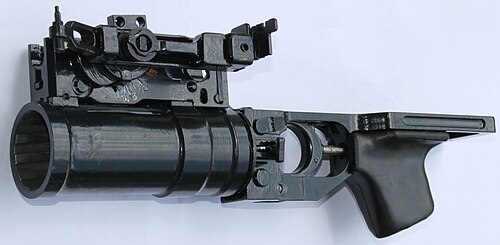
\includegraphics{../images/wyrzutnie_granatow/gp-30_1.jpg}
\caption{GP-30 Obuwka --- granatnik podlufowy}
\end{figure}

\subsection{Opis}\label{opis-95}

GP-30 Obuwka (Обувка --- Obuwie) to rosyjski nasadkowy granatnik podlufy
kalibru 40 mm opracowany przez KBP w Tule jako modernizacja GP-25 i
przyjęty do służby w 1989 roku. W stosunku do GP-25 jest lżejszy (1,0 kg
vs 1,5 kg) i ma ulepszone przyrządy celownicze --- folded-leaf sight po
lewej stronie z podziałką do 400 m. Zachowuje ładowanie od przodu
(muzzle-loading) i spust z tyłu, ale ma nowocześniejszą i ergonomiczną
rączkę. GP-30 jest standardowym nasadkowym granatnikiem na AK-74M i
AK-12 w armii rosyjskiej; stosowany przez wojsko i policję. Używa tej
samej amunicji 40 mm co GP-25 (VOG-25, VOG-25P itp.).

\subsection{Dane techniczne}\label{dane-techniczne-95}

\begin{longtable}[]{@{}ll@{}}
\toprule\noalign{}
Parametr & Wartość \\
\midrule\noalign{}
\endhead
\bottomrule\noalign{}
\endlastfoot
Typ & Nasadkowy granatnik podlufy \\
Kraj produkcji & Rosja \\
Rok wprowadzenia & 1989 \\
Kaliber & 40 mm \\
Długość & 276 mm \\
Masa (bez amunicji) & 1,0 kg \\
Zasięg maks. & 400 m \\
Prędkość wylotowa & 76 m/s \\
Szybkostrzelność & 4--5 strz./min \\
Obsługa & 1 osoba \\
\end{longtable}

\subsection{Charakterystyczne cechy
rozpoznawcze}\label{charakterystyczne-cechy-rozpoznawcze-95}

\begin{quote}
Jak odróżnić GP-30 od GP-25 i GP-34:
\end{quote}

\begin{itemize}
\tightlist
\item
  \textbf{Lżejszy i krótszy od GP-25 --- wyraźna różnica masy:} GP-30
  waży 1,0 kg vs 1,5 kg GP-25; przy przetrzymaniu jest wyraźnie lżejszy;
  jest też krótszy (276 mm vs 323 mm); pod lufą AK wygląda ``mniejszy''
  niż GP-25
\item
  \textbf{Nowszy, ergonomiczny kształt rączki spustowej:} GP-30 ma
  bardziej ergonomiczną ``przerębkę'' spustową niż GP-25; kształt
  uchwytu spustowego jest nowocześniejszy i lepiej dopasowany do dłoni w
  rękawicach
\item
  \textbf{Identyczne ładowanie od przodu jak GP-25 --- muzzle loading:}
  jak GP-25 i GP-34, GP-30 ładuje się od przodu lufy; ta cecha jest
  wspólna dla całej rosyjskiej rodziny granatników podlufy i odróżnia je
  od zachodnich (M203, AG36)
\item
  \textbf{Ulepszone przyrządy celownicze z ``listewką'' po lewej:} GP-30
  ma charakterystyczny składany listewkowy celownik po lewej stronie ---
  bardziej rozbudowany niż prosty celownik GP-25; skala odległości
  widoczna na celowniku
\item
  \textbf{Montaż kompatybilny z AK-74M i nowszymi AK:} GP-30 jest
  standardowym granatnikiem dla AK-74M i AK-12; jeśli widzimy nowoczesny
  AK z podlufą --- to prawdopodobnie GP-30, nie GP-25 (ten był na
  AKM/AK-74)
\item
  \textbf{Brak spustu z przodu --- identycznie jak GP-25:} spust GP-30
  jest z tyłu, przy chwycie karabinu; zachodnie granatniki (M203) mają
  spust z przodu podlufy; ta różnica w pozycji spustu identyfikuje całą
  rodzinę GP
\end{itemize}

\subsection{Ciekawostka}\label{ciekawostka-95}

\begin{quote}
GP-30 nosi przydomek ``Obuwka'' (obuwie) --- bo jego kształt i sposób
montażu na AK przypominają żartobliwie ``bucik'' zakładany na stopę
karabinu. Rosyjscy żołnierze, którzy dostawali AK-74M z GP-30, mówili,
że ``zakładają karabinowi but''. Żart przetrwał w slangu wojskowym do
dziś. GP-30 jest drugą co do popularności po GP-25 nasadką granatnikową
w armiach postsowieckich; różnicę ``GP-25 vs GP-30'' poznaje się
najprościej po masie i kształcie rączki spustowej.
\end{quote}

\section{Nasadkowy granatnik GP-34}\label{nasadkowy-granatnik-gp-34}

\subsubsection{GP-34 Underbarrel Grenade Launcher \textbar{}
ГП-34}\label{gp-34-underbarrel-grenade-launcher-ux433ux43f-34}

\begin{center}\rule{0.5\linewidth}{0.5pt}\end{center}

\begin{figure}
\centering
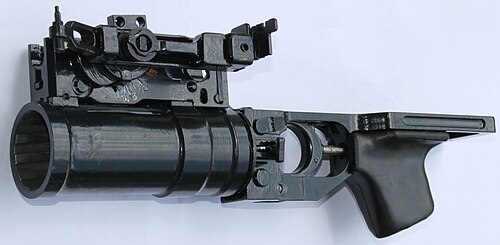
\includegraphics{../images/wyrzutnie_granatow/gp-34_1.jpg}
\caption{GP-34 --- granatnik podlufowy Ratnik}
\end{figure}

\subsection{Opis}\label{opis-96}

GP-34 to rosyjski nasadkowy granatnik podlufy kalibru 40 mm opracowany
przez KBP w Tule jako modernizacja GP-30 i zaprezentowany w 2000 roku.
Zachowuje ładowanie od przodu (muzzle-loading) i spust z tyłu jak
poprzedniki, ale dodaje możliwość montażu na karabinach AK bez demontażu
tylnicy magazynka --- co było problemem z GP-25/30. GP-34 ma
nowocześniejszy kształt i lepszą ergonomię; jest standardowym
wyposażeniem zestawu bojowego ``Ratnik'' (żołnierz przyszłości)
montowanym na AK-12 i AK-15. Używa tej samej amunicji VOG-25 co GP-25 i
GP-30.

\subsection{Dane techniczne}\label{dane-techniczne-96}

\begin{longtable}[]{@{}ll@{}}
\toprule\noalign{}
Parametr & Wartość \\
\midrule\noalign{}
\endhead
\bottomrule\noalign{}
\endlastfoot
Typ & Nasadkowy granatnik podlufy \\
Kraj produkcji & Rosja \\
Rok wprowadzenia & 2000 (Ratnik: 2015) \\
Kaliber & 40 mm \\
Długość & 280 mm \\
Masa (bez amunicji) & 1,1 kg \\
Zasięg maks. & 400 m \\
Szybkostrzelność & 4--5 strz./min \\
Obsługa & 1 osoba \\
\end{longtable}

\subsection{Charakterystyczne cechy
rozpoznawcze}\label{charakterystyczne-cechy-rozpoznawcze-96}

\begin{quote}
Jak odróżnić GP-34 od GP-30 i GP-25:
\end{quote}

\begin{itemize}
\tightlist
\item
  \textbf{Nowoczesny, kanciasty wygląd pasujący do AK-12:} GP-34 ma
  bardziej kanciastą, nowoczesną bryłę niż zaokrąglony GP-30; razem z
  AK-12 tworzy ``nowoczesny'' zestaw, podczas gdy GP-25/30 wyglądają
  ``staromodnie'' na AK-74M
\item
  \textbf{Widoczna w zestawie ``Ratnik'' --- na żołnierzach nowych
  formacji:} GP-34 pojawia się głównie na żołnierzach wyposażonych w
  pełny zestaw ``Ratnik'' (AK-12, kamizelka 6B45, hełm 6B47); starsze
  formacje mają GP-25 lub GP-30 na AK-74M
\item
  \textbf{Identyczne ładowanie od przodu i spust z tyłu:} jak całe
  GP-25/30 --- muzzle loading i spust z tyłu; te cechy są wspólne dla
  całej rodziny i odróżniają ją od zachodnich M203
\item
  \textbf{Nieco cięższy od GP-30 (1,1 kg vs 1,0 kg) --- prawie
  nieodróżnialny masą:} różnica masy między GP-30 a GP-34 jest
  minimalna; praktycznie identyczne w ręce; różnicuje je głównie kształt
  i kompatybilność z konkretnym modelem AK
\item
  \textbf{Celownik listewkowy po lewej --- identyczny układ jak GP-30:}
  celownik GP-34 wygląda bardzo podobnie do GP-30; skala listewkowa po
  lewej stronie; subtelna różnica w kształcie obudowy celownika
\item
  \textbf{Rzadziej widoczny niż GP-25 i GP-30 --- nowszy system:} GP-34
  jest stosunkowo nowy i pojawia się głównie w zdjęciach elitarnych
  jednostek lub materiałach z zestawem ``Ratnik''; GP-25 i GP-30 są
  znacznie powszechniejsze na polach walki
\end{itemize}

\subsection{Ciekawostka}\label{ciekawostka-96}

\begin{quote}
GP-34 jest integralną częścią zestawu ``Ratnik'' --- rosyjskiego
programu ``żołnierza przyszłości'' --- i jest pierwszym rosyjskim
granatnikiem nasadkowym, który ``od projektowania'' był przewidziany do
pracy z elektronicznym celownikiem i cyfrowym interfejsem bojowym
zestawu Ratnik. Poprzednie modele (GP-25, GP-30) były ``dokładane'' do
karabinów jako dodatek; GP-34 jest elementem zintegrowanego systemu
bojowego. W teorii GP-34 powinien był zastąpić GP-25 i GP-30 masowo ---
w praktyce tempo dostaw zestawów Ratnik jest wolniejsze niż planowano i
starsze GP-25/30 wciąż dominują na froncie.
\end{quote}

\section{Automatyczny granatnik AGS-17
Płamia}\label{automatyczny-granatnik-ags-17-pux142amia}

\subsubsection{AGS-17 Plamya Automatic Grenade Launcher \textbar{}
АГС-17
«Пламя»}\label{ags-17-plamya-automatic-grenade-launcher-ux430ux433ux441-17-ux43fux43bux430ux43cux44f}

\begin{center}\rule{0.5\linewidth}{0.5pt}\end{center}

\begin{figure}
\centering
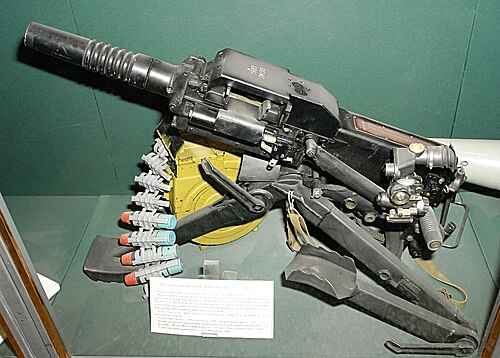
\includegraphics{../images/wyrzutnie_granatow/ags-17_1.jpg}
\caption{AGS-17 Płamia --- automatyczny granatnik 30 mm}
\end{figure}

\subsection{Opis}\label{opis-97}

AGS-17 Płamia (Пламя --- Płomień) to radziecki automatyczny granatnik
stanowiskowy kalibru 30 mm opracowany przez KBP w Tule i przyjęty do
służby w 1971 roku. Strzela seryjnie granatami odłamkowo-burzącymi
VOG-17M na odległość do 1730 m --- zapewniając nasycenie obszaru
odłamkami jak moździerz, ale z szybkostrzelnością automatyczną (50--65
strzałów/min). AGS-17 jest montowany na trójnodze naziemnym, BWP
(BMP-2), śmigłowcach (Mi-24) i łodziach bojowych. Obsługa 3-osobowa może
przenosić rozkładany zestaw na plecach. Szeroko stosowany w
Afganistanie, Czeczenii, Syrii i na Ukrainie --- jest standardową bronią
wsparcia szczebla kompania w armii rosyjskiej.

\subsection{Dane techniczne}\label{dane-techniczne-97}

\begin{longtable}[]{@{}ll@{}}
\toprule\noalign{}
Parametr & Wartość \\
\midrule\noalign{}
\endhead
\bottomrule\noalign{}
\endlastfoot
Typ & Automatyczny granatnik stanowiskowy \\
Kraj produkcji & ZSRR / Rosja \\
Rok wprowadzenia & 1971 \\
Kaliber & 30×29 mm \\
Długość (bez trójnogu) & 840 mm \\
Masa (z trójnogiem i bębnem) & 31 kg \\
Zasięg maks. & 1 730 m \\
Szybkostrzelność & 50--65 strz./min \\
Pojemność zasobnika & 29 nabojów (bęben) \\
Obsługa & 3 osoby \\
\end{longtable}

\subsection{Charakterystyczne cechy
rozpoznawcze}\label{charakterystyczne-cechy-rozpoznawcze-97}

\begin{quote}
Jak odróżnić AGS-17 od AGS-30 i granatników Mk 19:
\end{quote}

\begin{itemize}
\tightlist
\item
  \textbf{Charakterystyczny okrągły bębnowy zasobnik nabojowy z lewej
  strony:} AGS-17 ma charakterystyczny okrągły metalowy bęben z nabojami
  (29 sztuk) przymocowany po lewej stronie broni; ten okrągły zasobnik
  jest natychmiastowym identyfikatorem --- żadna inna broń nie ma tak
  widocznego okrągłego bębna z boku
\item
  \textbf{Prostokątna skrzynkowa komora zamkowa --- ``pudełkowaty''
  wygląd:} AGS-17 ma charakterystyczny ``pudełkowy'' kształt komory
  zamkowej i korpusu; przypomina bardziej maszynę przemysłową niż typowy
  karabin; ten geometryczny, kanciasty wygląd odróżnia go od lżejszego
  AGS-30
\item
  \textbf{Trójnóg z regulacją wysokości --- stalowe nogi o ``pajęczym''
  układzie:} trójnóg AGS-17 ma charakterystyczne trzy grube stalowe nogi
  z regulacją; całość jest masywna i wyraźnie ``wojskowa''; podobnie do
  trójnogu DShK, ale mniejszy
\item
  \textbf{Masywny, ciężki zestaw --- 31 kg całości:} AGS-17 z trójnogiem
  i zasobnikiem waży 31 kg; AGS-30 jest lżejszy (16 kg); przy
  transporcie widać ciężar zestawu --- 3 osoby niosą go w częściach
\item
  \textbf{Montaż na BWP i śmigłowcach --- widoczna na pojazdach:} AGS-17
  na wieżyczce BWP lub pod dziobem Mi-24 to rozpoznawalny widok; mały,
  kanciasty granatnik ze swoim bębnem jest charakterystycznym
  wyposażeniem tych platform
\item
  \textbf{Linia ognia prawie pozioma --- nie jak moździerz, nie jak
  karabin:} AGS-17 strzela pod małym kątem elevacji (jak karabin), a nie
  bardzo stromo (jak moździerz); żołnierz ``celuje'' jak z karabinu
  maszynowego, nie jak z moździerza
\end{itemize}

\subsection{Ciekawostka}\label{ciekawostka-97}

\begin{quote}
AGS-17 zyskał sławę w Afganistanie, gdzie radzieccy żołnierze montowali
go na dachach budynków i ścianach okopów zamiast na trójnogu ---
``pionowy'' AGS-17 strzelał jak moździerz, rażąc cele za wzniesieniami
terenu. Ten pomysłowy sposób użycia nie był przewidziany przez
projektantów, ale okazał się bardzo skuteczny w górach, gdzie tradycyjne
``płaskie'' strzelanie granatamiutrudniała rzeźba terenu. Afgańscy
mudżahedini zdobywali AGS-17 i przechowywali je jako cenne łupy --- bo
granat VOG-17M eksploduje nawet przy kontakcie z cienką gałązką drzewa.
\end{quote}

\section{Automatyczny granatnik
AGS-30}\label{automatyczny-granatnik-ags-30}

\subsubsection{AGS-30 Automatic Grenade Launcher \textbar{}
АГС-30}\label{ags-30-automatic-grenade-launcher-ux430ux433ux441-30}

\begin{center}\rule{0.5\linewidth}{0.5pt}\end{center}

\begin{figure}
\centering
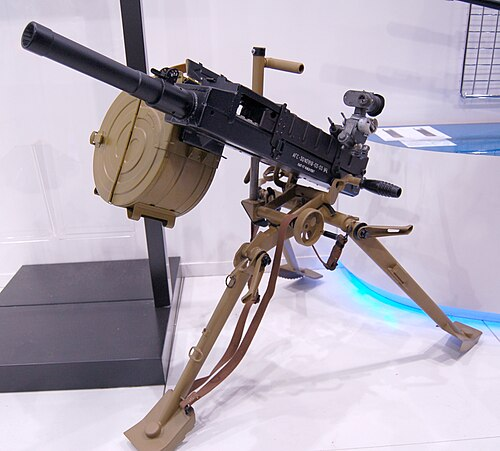
\includegraphics{../images/wyrzutnie_granatow/ags-30_1.jpg}
\caption{AGS-30 --- automatyczny granatnik 30 mm}
\end{figure}

\subsection{Opis}\label{opis-98}

AGS-30 to rosyjski automatyczny granatnik stanowiskowy kalibru 30 mm
opracowany przez KBP w Tule jako lżejszy następnik AGS-17 i przyjęty do
służby w 1995 roku. Wyróżnia się masą o połowę mniejszą niż AGS-17 ---
16 kg całości vs 31 kg --- co pozwala na przeniesienie zestawu przez
dwie osoby zamiast trzech. Używa ulepszonej amunicji VOG-30 (w tym
VOG-30P z zapalnikiem zdalnym) i ma wyższy zasięg niż AGS-17. AGS-30
jest coraz szerzej stosowany jako uzupełnienie i następca AGS-17 w armii
rosyjskiej; pojawia się na Ukrainie jako przenośna broń wsparcia
piechoty i na pojazdach.

\subsection{Dane techniczne}\label{dane-techniczne-98}

\begin{longtable}[]{@{}ll@{}}
\toprule\noalign{}
Parametr & Wartość \\
\midrule\noalign{}
\endhead
\bottomrule\noalign{}
\endlastfoot
Typ & Automatyczny granatnik stanowiskowy \\
Kraj produkcji & Rosja \\
Rok wprowadzenia & 1995 \\
Kaliber & 30×29 mm \\
Długość & 825 mm \\
Masa (z trójnogiem) & 16 kg \\
Zasięg maks. & 1 700 m \\
Szybkostrzelność & 400 strz./min (max) / 60 strz./min (bojowy) \\
Pojemność taśmy & 30 nabojów \\
Obsługa & 2 osoby \\
\end{longtable}

\subsection{Charakterystyczne cechy
rozpoznawcze}\label{charakterystyczne-cechy-rozpoznawcze-98}

\begin{quote}
Jak odróżnić AGS-30 od AGS-17:
\end{quote}

\begin{itemize}
\tightlist
\item
  \textbf{Wyraźnie mniejszy i lżejszy od AGS-17 --- 16 kg vs 31 kg:}
  AGS-30 jest niemal o połowę lżejszy; przy porównaniu sylwetek na
  zdjęciach AGS-30 jest smuklejszy i ``mniejszy''; trójnóg jest też
  lżejszy i cieńszy
\item
  \textbf{Taśmowe podawanie amunicji zamiast bębna:} AGS-30 ma zasilanie
  taśmowe (kaseta z taśmą) zamiast okrągłego bębna AGS-17; brak
  charakterystycznego okrągłego zasobnika po lewej jest kluczowym
  wyróżnikiem; zamiast bębna widoczna jest kaseta z taśmą
\item
  \textbf{Bardziej opływowy, nowocześniejszy wygląd komory zamkowej:}
  AGS-30 ma nowocześniejszy, mniej ``pudełkowaty'' kształt niż AGS-17;
  sylwetka jest bardziej opływowa i nowoczesna
\item
  \textbf{Cieńsze nogi trójnogu i lżejszy montaż:} trójnóg AGS-30 jest
  wyraźnie cieńszy i lżejszy od masywnego trójnogu AGS-17; cała
  platforma sprawia wrażenie ``nowocześ­niejszej'' i ``lekkości''
\item
  \textbf{Obsługa 2-osobowa zamiast 3-osobowej:} AGS-30 obsługują 2
  osoby; AGS-17 --- 3; przy obserwacji pracy obsługi różnica w liczbie
  ludzi to sygnał
\item
  \textbf{Kaseta taśmowa z boku --- inny układ zasilania niż AGS-17:}
  przy AGS-30 widoczna jest kaseta z taśmą (mniej widowiskowy niż
  okrągły bęben); ta różnica układu podajnika jest kluczowa
\end{itemize}

\subsection{Ciekawostka}\label{ciekawostka-98}

\begin{quote}
AGS-30 projektowano z założeniem, że żołnierz będzie go przenosić sam
lub we dwójkę bez pojazdu. W testach jeden wytrenowany żołnierz mógł
dźwigać cały AGS-30 rozkładany w plecaku --- czego nigdy nie osiągnięto
z AGS-17. W Syrii rosyjscy doradcy wojskowi wyposażali syryjskie
jednostki specjalne w AGS-30 jako ``mobilne wsparcie ogniowe'' w
miastach --- cięższy AGS-17 był za mało manewrowy do walk ulicznych.
Lżejszy AGS-30 okazał się idealny do szybkich zasadzek: rozłożenie,
seria i odejście przed kontratakiem.
\end{quote}

\section{Automatyczny granatnik AGS-40
Bałkan}\label{automatyczny-granatnik-ags-40-baux142kan}

\subsubsection{AGS-40 Balkan Automatic Grenade Launcher \textbar{}
АГС-40
«Балкан»}\label{ags-40-balkan-automatic-grenade-launcher-ux430ux433ux441-40-ux431ux430ux43bux43aux430ux43d}

\begin{center}\rule{0.5\linewidth}{0.5pt}\end{center}

\begin{figure}
\centering
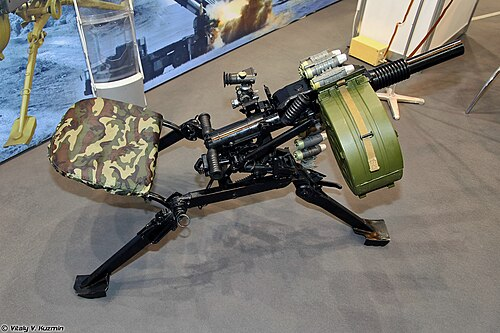
\includegraphics{../images/wyrzutnie_granatow/ags-40_1.jpg}
\caption{AGS-40 Bałkan --- automatyczny granatnik 40 mm}
\end{figure}

\subsection{Opis}\label{opis-99}

AGS-40 Bałkan (Балкан) to rosyjski automatyczny granatnik stanowiskowy
kalibru 40 mm opracowany przez KBP w Tule i przyjęty do służby ok. 2018
roku jako broń nowej generacji dla programu ``Ratnik-3''. Wyróżnia się
kaliber 40 mm (większy niż 30 mm AGS-17/30) z nową amunicją ZOF-40 o
znacznie większej masie głowicy i zasięgu do 2500 m. Nowa amunicja Z-40
ma możliwość programowania zapalnika ``na odległość'' (airburst) ---
granat wybucha w powietrzu nad okopem lub za zasłoną. AGS-40 jest
cięższy od AGS-30, ale daje znacznie większą siłę rażenia. Trwa
doposażanie wybranych jednostek.

\subsection{Dane techniczne}\label{dane-techniczne-99}

\begin{longtable}[]{@{}ll@{}}
\toprule\noalign{}
Parametr & Wartość \\
\midrule\noalign{}
\endhead
\bottomrule\noalign{}
\endlastfoot
Typ & Automatyczny granatnik stanowiskowy nowej generacji \\
Kraj produkcji & Rosja \\
Rok wprowadzenia & ok. 2018 \\
Kaliber & 40×53 mm \\
Masa (z trójnogiem) & \textasciitilde32 kg \\
Zasięg maks. & 2 500 m \\
Szybkostrzelność & 400 strz./min (max) / 60--100 strz./min (bojowy) \\
Obsługa & 2--3 osoby \\
\end{longtable}

\subsection{Charakterystyczne cechy
rozpoznawcze}\label{charakterystyczne-cechy-rozpoznawcze-99}

\begin{quote}
Jak odróżnić AGS-40 od AGS-17 i AGS-30:
\end{quote}

\begin{itemize}
\tightlist
\item
  \textbf{Wyraźnie grubsza rura lufy 40 mm --- kaliber 40 vs 30 mm
  widoczny:} lufa AGS-40 ma kaliber 40 mm --- wyraźnie grubsza niż lufa
  AGS-17/30 (30 mm); przy porównaniu obu broni grubość lufy od razu
  odróżnia AGS-40
\item
  \textbf{Nowoczesny wygląd --- kanciasty, taktyczny design z szynami:}
  AGS-40 ma nowoczesny wygląd z szynami Picatinny i ergonomicznym łożem
  --- bardziej ``taktyczny'' niż ``wojskowy retro'' AGS-17; wyraźna
  różnica w stylistyce
\item
  \textbf{Brak okrągłego bębna --- taśmowe podawanie:} AGS-40 (jak
  AGS-30) ma taśmowe zasilanie bez charakterystycznego okrągłego bębna
  AGS-17; kaseta z taśmą z boku
\item
  \textbf{Rzadkość na polu walki --- nowa broń z ograniczoną produkcją:}
  AGS-40 jest nowym systemem i pojawia się rzadko; jego widok sugeruje
  jednostkę wyposażoną w sprzęt ``Ratnik-3''; powszechniejszy AGS-17 i
  AGS-30 są na starszych formacjach
\item
  \textbf{Cięższy od AGS-30 --- ok. 32 kg (podobny do AGS-17):} AGS-40
  waży więcej niż AGS-30; masa jest bliższa AGS-17; to ``powrót'' do
  ciężkiej platformy po lżejszym AGS-30 --- za cenę większej siły
  rażenia
\item
  \textbf{Programowalny zapalnik --- widoczny dodatkowy element
  elektroniczny przy lufie:} wersje z programowalnym zapalnikiem
  airburst mają dodatkowy moduł elektroniczny przy wyjściu lufy lub
  komoże --- charakterystyczny ``kwadratowy element'' nieobecny w
  AGS-17/30
\end{itemize}

\subsection{Ciekawostka}\label{ciekawostka-99}

\begin{quote}
AGS-40 Bałkan jest pierwszym rosyjskim automatycznym granatnikiem
stanowiskowym zdolnym do strzelania pociskami airburst --- granaty
eksplodują w zaprogramowanej odległości w powietrzu, rażąc cel ``z
góry'' odłamkami. Ta technika szczególnie skutecznie niszczy siłę żywą w
okopach i za osłonami, gdzie tradycyjne granaty wybuchające przy
trafieniu są mniej efektywne. Zachodnie odpowiedniki (Mk 47 Striker)
mają tę samą funkcję od lat, ale AGS-40 jest pierwszym rosyjskim
granatnikiem z tą zdolnością --- demonstrując, że Rosja nadrabia
zaległości technologiczne w tej dziedzinie.
\end{quote}

\section{Rewolwerowy granatnik GM-94}\label{rewolwerowy-granatnik-gm-94}

\subsubsection{GM-94 Pump-Action Grenade Launcher \textbar{}
ГМ-94}\label{gm-94-pump-action-grenade-launcher-ux433ux43c-94}

\begin{center}\rule{0.5\linewidth}{0.5pt}\end{center}

\begin{figure}
\centering
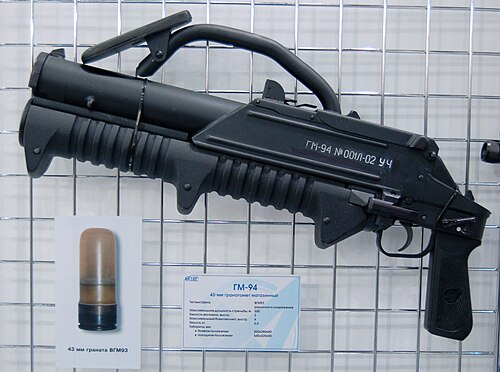
\includegraphics{../images/wyrzutnie_granatow/gm-94_1.jpg}
\caption{GM-94 --- rewolwerowy granatnik pump-action}
\end{figure}

\subsection{Opis}\label{opis-100}

GM-94 to rosyjski rewolwerowy granatnik pompowy (pump-action) kalibru 43
mm opracowany przez KBP w Tule i przyjęty do służby w 1994 roku dla FSB,
jednostek antyterrorystycznych i sił specjalnych. Wyróżnia się
kompaktową budową i bębnowym magazynkiem na 3 naboje --- może strzelać
różnymi typami amunicji: termobaryczną (OD-43), chemiczną (drażniąca),
dymną, gumową (nieśmiertelna) i odłamkową. Ruch pompowy ``przerucza''
nabój i gotuje broń do strzału --- podobnie jak shotgun. GM-94 jest
przeznaczony do walki w budynkach i tunelach na bliskie odległości (do
300 m) --- nie do strzelania artyleryjskiego. Uważany za jedno z
najlepszych narzędzi antyterrorystycznych na świecie.

\subsection{Dane techniczne}\label{dane-techniczne-100}

\begin{longtable}[]{@{}ll@{}}
\toprule\noalign{}
Parametr & Wartość \\
\midrule\noalign{}
\endhead
\bottomrule\noalign{}
\endlastfoot
Typ & Rewolwerowy granatnik pump-action \\
Kraj produkcji & Rosja \\
Rok wprowadzenia & 1994 \\
Kaliber & 43 mm \\
Długość & 810 mm \\
Masa (bez nabojów) & 4,8 kg \\
Pojemność & 3 naboje (bęben) + 1 w komorze \\
Zasięg maks. & 300 m \\
Szybkostrzelność & 6--8 strz./min (pump-action) \\
Obsługa & 1 osoba \\
\end{longtable}

\subsection{Charakterystyczne cechy
rozpoznawcze}\label{charakterystyczne-cechy-rozpoznawcze-100}

\begin{quote}
Jak odróżnić GM-94 od GP-25/30 i AGS-17:
\end{quote}

\begin{itemize}
\tightlist
\item
  \textbf{Autonomiczna broń strzelecka --- nie nasadkowy granatnik:}
  GM-94 to samodzielna broń, nie montowana pod lufą karabinu; ma własną
  kolbę, spust i chwyt --- wygląda jak duży shotgun, nie jak nasadkowa
  wyrzutnia; to fundamentalna różnica od GP-25/30
\item
  \textbf{Bęben na 3 naboje widoczny pod rurą magazynkową:} GM-94 ma
  charakterystyczny okrągły magazynek-bęben z 3 nabojami widoczny pod
  rurą; ruch pompowy (przesunięcie cześć przedniej ku tyłowi) powoduje
  obrót bębna i załadowanie kolejnego naboju
\item
  \textbf{Kaliber 43 mm --- unikalny, niespotykany w innych rosyjskich
  granatnikach:} kaliber 43 mm jest charakterystyczny tylko dla GM-94;
  GP-25/30/34 mają 40 mm; AGS-17/30 mają 30 mm; niezwykły kaliber 43 mm
  identyfikuje GM-94 jednoznacznie
\item
  \textbf{Wygląd ``pompowego strzelby'' --- nie karabinu ani
  stanowiskowej broni:} GM-94 wygląda jak grubszy shotgun z pumpa; żadna
  inna rosyjska broń nie ma tak ``cywilnego'' lub ``policyjnego''
  wyglądu --- GM-94 nie wygląda jak wojskowy granatnik
\item
  \textbf{Kompaktowy i stosowany przez policję oraz antyterrorystów:}
  GM-94 pojawia się głównie na fotografiach FSB, OMON i rosyjskich
  jednostek antyterrorystycznych --- nie na regularnych żołnierzach
  piechoty; sam kontekst użycia sugeruje tę broń
\item
  \textbf{Różnorodna amunicja --- widoczne różne kolory głowic nabojów:}
  naboje GM-94 mają różne kolory w zależności od przeznaczenia
  (termobaryczny, gumowy, dymny) --- przy obserwacji obsługi strzelec
  dobiera ``kolor naboju'' odpowiedni do sytuacji; ten dobór amunicji
  jest charakterystyczny dla broni wielozadaniowej
\end{itemize}

\subsection{Ciekawostka}\label{ciekawostka-100}

\begin{quote}
GM-94 był jednym z narzędzi używanych przez FSB podczas szturmu na teatr
na Dubrowce w 2002 roku (zakładnicy Nord-Ost). Według niepotwierdzonych
raportów, GM-94 z amunicją chemiczną (środek powodujący chwilowy
paraliż) był testowany w scenariuszach szturmu budynku --- jako sposób
na obezwładnienie terrorystów bez zabijania zakładników. Skuteczność w
tamtym konkretnym zdarzeniu jest dyskutowana, bo większość ofiar
zakładniczych zginęła od środka znieczulającego przez wentylację, nie od
bezpośredniego działania broni.
\end{quote}

\section{Pistolet Makarowa PM}\label{pistolet-makarowa-pm}

\subsubsection{Makarov PM Pistol \textbar{} ПМ (Пистолет
Макарова)}\label{makarov-pm-pistol-ux43fux43c-ux43fux438ux441ux442ux43eux43bux435ux442-ux43cux430ux43aux430ux440ux43eux432ux430}

\begin{center}\rule{0.5\linewidth}{0.5pt}\end{center}

\begin{figure}
\centering
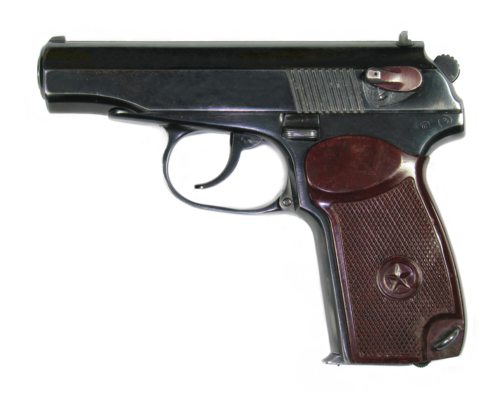
\includegraphics{../images/pistolety_i_pm/pm_1.jpg}
\caption{Pistolet PM Makarow}
\end{figure}

\subsection{Opis}\label{opis-101}

PM (Пистолет Макарова --- Pistolet Makarowa) to radziecki pistolet
samopowtarzalny kalibru 9×18 mm Makarov zaprojektowany przez Nikołaja
Makarowa i przyjęty do służby w 1951 roku jako zastępnik Pistoletu TT.
Jest jednym z najszerzej produkowanych pistoletów w historii --- szacuje
się ponad 5 milionów egzemplarzy. Prosta, niezawodna i tania w produkcji
konstrukcja z podwójnym działaniem spustu (DA/SA) sprawiła, że PM stał
się standardowym pistoletem wojskowym i policyjnym ZSRR, a następnie
wszystkich krajów Układu Warszawskiego --- w tym Polski. Mimo
oficjalnego zastąpienia przez MP-443 Grach, PM jest nadal powszechnie
używany w rosyjskiej policji, służbach i wojskach rezerwowych.

\subsection{Dane techniczne}\label{dane-techniczne-101}

\begin{longtable}[]{@{}ll@{}}
\toprule\noalign{}
Parametr & Wartość \\
\midrule\noalign{}
\endhead
\bottomrule\noalign{}
\endlastfoot
Typ & Pistolet samopowtarzalny \\
Kraj produkcji & ZSRR / Rosja \\
Rok wprowadzenia & 1951 \\
Kaliber & 9×18 mm Makarov \\
Długość & 161 mm \\
Długość lufy & 93 mm \\
Masa (bez magazynka) & 730 g \\
Pojemność magazynka & 8 nabojów \\
Prędkość wylotowa & 315 m/s \\
Skuteczny zasięg & 50 m \\
\end{longtable}

\subsection{Charakterystyczne cechy
rozpoznawcze}\label{charakterystyczne-cechy-rozpoznawcze-101}

\begin{quote}
Jak odróżnić PM od TT, MP-443 i pistoletów zachodnich:
\end{quote}

\begin{itemize}
\tightlist
\item
  \textbf{Mała, kompaktowa sylwetka --- wyraźnie mniejszy od MP-443 i
  TT:} PM jest wyraźnie mniejszy i lżejszy od nowszego MP-443 Grach;
  przy porównaniu proporcje są ``minipistoletu''; mniejszy też od TT
  (który jest większy i bardziej kanciast)
\item
  \textbf{Charakterystyczna okrągła ``pętla'' spustu i estetyka lat
  50.:} PM ma charakterystyczny zaokrąglony spust w prostokątnej
  kabłąkowej ramie; ogólna estetyka jest zaokrąglona i ``miękka'' ---
  typowa dla projektów lat 50.; MP-443 jest kanciasty i nowoczesny
\item
  \textbf{Zewnętrzny kurek (hammer) z tyłu slajdu:} PM ma wyraźny
  zewnętrzny kurek z tyłu zamka (slide); naciąganie PM jest widoczne;
  pistolety bez widocznego kurka (jak Glock) wyglądają inaczej
\item
  \textbf{Mały, prosty celownik bez podświetlenia:} PM ma
  minimalistyczny stały celownik bez żadnych nacięć białych punktów, bez
  podświetlenia; nowoczesne pistolety mają rozbudowane systemy
  celownicze
\item
  \textbf{Magazynek 8-nabojowy --- wyraźnie węższy niż MP-443 (17
  nabojów):} magazynek PM jest wąski (8 nabojów jednorzędowych);
  magazynek MP-443 jest szerszy (17 nabojów dwurzędowych); różnica
  szerokości chwytu jest widoczna
\item
  \textbf{Brak szyny Picatinny --- gładka rama pod lufą:} PM nie ma
  szyny do latarki czy celownika laserowego; gładki dół ramy to cecha
  ``starego'' pistoletu; MP-443 i nowsze pistolety mają szynę
\end{itemize}

\subsection{Ciekawostka}\label{ciekawostka-101}

\begin{quote}
PM przez długie lata był ``pistoletem wrogów i przyjaciół'' jednocześnie
--- każdy kraj NATO miał w swoich arsenałach zdobyczne PM, bo były tak
powszechne, że trafiały do wszystkich. Izraelskie służby bezpieczeństwa
używały zdobycznych PM przez dekady. CIA miała zapasy PM ``do operacji
pod fałszywą flagą''. Paradoksalnie, PM jest tak prosty, że produkuje go
dziś wiele firm komercyjnych dla kolekcjonerów zachodnich --- czyniąc z
radzieckiego pistoletu wojskowego popularny eksponat w prywatnych
kolekcjach USA.
\end{quote}

\section{Pistolet TT (Tulski
Tokariew)}\label{pistolet-tt-tulski-tokariew}

\subsubsection{TT (Tokarev) Pistol \textbar{} ТТ (Тульский
Токарев)}\label{tt-tokarev-pistol-ux442ux442-ux442ux443ux43bux44cux441ux43aux438ux439-ux442ux43eux43aux430ux440ux435ux432}

\begin{center}\rule{0.5\linewidth}{0.5pt}\end{center}

\begin{figure}
\centering
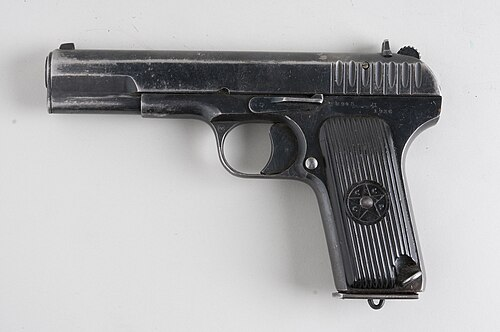
\includegraphics{../images/pistolety_i_pm/tt_1.jpg}
\caption{Pistolet TT Tokariew}
\end{figure}

\subsection{Opis}\label{opis-102}

TT (Тульский Токарев --- Tulski Tokariew) to radziecki pistolet
samopowtarzalny kalibru 7,62×25 mm TT zaprojektowany przez Fiodora
Tokarjewa i przyjęty do służby w 1930 roku (TT-30) oraz 1933 roku
(ulepszony TT-33). Charakteryzuje się prostą, niezawodną konstrukcją i
bardzo energetycznym nabojem 7,62×25 mm --- pocisk przenikający
kamizelki balistyczne klasy I-II. TT był standardowym pistoletem wojska
i NKWD/KGB przez II wojnę światową i wiele lat po niej; zastąpiony przez
PM dopiero w 1951 roku. Mimo oficjalnego wycofania TT jest powszechny w
krajach byłego ZSRR, Chinach (kopia Typ 54), Jugosławii i dziesiątkach
innych krajów --- i regularnie pojawia się w konfliktach zbrojnych.

\subsection{Dane techniczne}\label{dane-techniczne-102}

\begin{longtable}[]{@{}ll@{}}
\toprule\noalign{}
Parametr & Wartość \\
\midrule\noalign{}
\endhead
\bottomrule\noalign{}
\endlastfoot
Typ & Pistolet samopowtarzalny \\
Kraj produkcji & ZSRR \\
Rok wprowadzenia & 1930 (TT-30) / 1933 (TT-33) \\
Kaliber & 7,62×25 mm TT \\
Długość & 194 mm \\
Długość lufy & 116 mm \\
Masa (bez magazynka) & 854 g \\
Pojemność magazynka & 8 nabojów \\
Prędkość wylotowa & 420 m/s \\
Skuteczny zasięg & 50 m \\
\end{longtable}

\subsection{Charakterystyczne cechy
rozpoznawcze}\label{charakterystyczne-cechy-rozpoznawcze-102}

\begin{quote}
Jak odróżnić TT od PM i pistoletów zachodnich:
\end{quote}

\begin{itemize}
\tightlist
\item
  \textbf{Wyraźnie większy i dłuższy od PM --- bardziej ``karabinowy''
  profil:} TT jest wyraźnie dłuższy (194 mm vs 161 mm PM) i
  masywniejszy; przy porównaniu TT sprawia wrażenie ``pistoletu z innej
  epoki'' --- bardziej kanciasowego i prostokątnego
\item
  \textbf{Brak zewnętrznego zabezpieczenia na zamku --- tylko
  wewnętrzne:} TT nie ma dźwigni bezpiecznika na zewnątrz ramy (jak PM
  czy MP-443); to niebezpieczne w codziennym noszeniu --- był to jeden z
  powodów zastąpienia go przez PM; brak zewnętrznego bezpiecznika jest
  widoczny
\item
  \textbf{Płaskie, drewniane lub bakelitowe okładziny chwytu:} TT ma
  charakterystyczne płaskie okładziny z drewna lub bakelitu z reliefem w
  kształcie gwiazdki radzieckiej; PM ma gumowe lub plastikowe okładziny;
  stare drewniane okladziny TT są odróżnialne wizualnie
\item
  \textbf{Wyraźna linia ``zamka'' (slide) biegąca poziomo wzdłuż górnej
  części:} TT ma charakterystyczny długi, prostokątny zamek z widocznymi
  rowkami ryflowania na tylnej części do naciągania; profil zamka jest
  bardzo geometryczny i ``retro''
\item
  \textbf{Nabój 7,62×25 mm --- smuklejszy i dłuższy niż 9×18 mm PM:}
  nabój TT jest wyraźnie dłuższy i smuklejszy od naboju PM; przy
  obserwacji załadowania widać mniejszy kaliber a większą długość
  naboju; bardzo charakterystyczny wygląd amunicji
\item
  \textbf{Brak szyny montażowej i żadnych nowoczesnych elementów:} TT
  nie ma szyn, nie ma celowników regulowanych, nie ma podświetlanych
  przyrządów; prosta archaiczna estetyka broni z lat 30. odróżnia od
  każdego nowoczesnego pistoletu
\end{itemize}

\subsection{Ciekawostka}\label{ciekawostka-102}

\begin{quote}
TT zyskał niechlubną sławę jako ``ulubiony pistolet przestępców'' w
Rosji i krajach byłego ZSRR lat 90. --- bo był tani, dostępny na czarnym
rynku i przebijał ówczesne kamizelki policyjne. Rosyjscy policjanci byli
dosłownie gorzej uzbrojeni niż przestępcy: policja miała PM (chroniony
przed kamizelką I klasy), a zorganizowane grupy przestępcze --- TT
(przebijający kamizelki klasy II). Ta sytuacja przyspieszyła
modernizację uzbrojenia rosyjskiej policji w latach 2000. i wprowadzenie
MP-443 Grach.
\end{quote}

\section{Pistolet maszynowy APS
(Steczkin)}\label{pistolet-maszynowy-aps-steczkin}

\subsubsection{APS Stechkin Machine Pistol \textbar{} АПС
(Автоматический Пистолет
Стечкина)}\label{aps-stechkin-machine-pistol-ux430ux43fux441-ux430ux432ux442ux43eux43cux430ux442ux438ux447ux435ux441ux43aux438ux439-ux43fux438ux441ux442ux43eux43bux435ux442-ux441ux442ux435ux447ux43aux438ux43dux430}

\begin{center}\rule{0.5\linewidth}{0.5pt}\end{center}

\begin{figure}
\centering
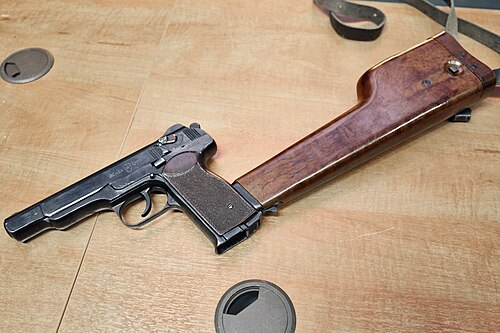
\includegraphics{../images/pistolety_i_pm/aps_1.jpg}
\caption{APS Steczkin --- pistolet maszynowy}
\end{figure}

\subsection{Opis}\label{opis-103}

APS (Автоматический Пистолет Стечкина --- Automatyczny Pistolet
Stieczkina) to radziecki pistolet maszynowy-pistolet kalibru 9×18 mm
zaprojektowany przez Igora Stieczkina i przyjęty do służby w 1951 roku.
Wyróżnia się możliwością prowadzenia ognia automatycznego (750
strz./min) przy użyciu odpinanej kolby-kabury jako stabilizatora.
Magazynek 20-nabojowy i ogień automatyczny czynią z APS broń pośrednią
między pistoletem a pistoletem maszynowym --- przeznaczoną dla oficerów,
artylerzystów, załóg pojazdów i sił specjalnych. Oficjalnie wycofany z
regularnej służby w 1958 roku ze względu na masę i rozmiary, APS
powrócił w latach 80.--90. i jest nadal używany przez siły specjalne i
FSB. Posiada kultowy status w popkulturze rosyjskiej.

\subsection{Dane techniczne}\label{dane-techniczne-103}

\begin{longtable}[]{@{}ll@{}}
\toprule\noalign{}
Parametr & Wartość \\
\midrule\noalign{}
\endhead
\bottomrule\noalign{}
\endlastfoot
Typ & Pistolet maszynowy / pistolet automatyczny \\
Kraj produkcji & ZSRR / Rosja \\
Rok wprowadzenia & 1951 \\
Kaliber & 9×18 mm Makarov \\
Długość (bez kolby) & 225 mm \\
Długość (z kolbą złożoną) & 540 mm \\
Długość lufy & 140 mm \\
Masa (bez magazynka) & 1 020 g \\
Pojemność magazynka & 20 nabojów \\
Szybkostrzelność & 750 strz./min (automatycznie) \\
Skuteczny zasięg & 50 m (pistolet) / 150 m (z kolbą) \\
\end{longtable}

\subsection{Charakterystyczne cechy
rozpoznawcze}\label{charakterystyczne-cechy-rozpoznawcze-103}

\begin{quote}
Jak odróżnić APS od PM i pistoletów maszynowych:
\end{quote}

\begin{itemize}
\tightlist
\item
  \textbf{Wyraźnie większy i dłuższy od PM --- rozmiar ``dużego
  pistoletu'':} APS jest wyraźnie większy od PM --- dłuższa lufa (140 mm
  vs 93 mm), wyższy chwyt, cięższy; przy noszeniu w kaburze widoczny
  jest ``dużego pistoletu'' profil
\item
  \textbf{Dźwignia trybu ognia (selektywny ogień) po lewej stronie
  slajdu:} APS ma charakterystyczną dźwignię trybu ognia (semi / auto)
  po lewej stronie zamka --- widoczna metalowa dźwignia z oznaczeniami;
  PM nie ma selektora ognia
\item
  \textbf{Odpinaną kolba-kabura z tyłu chwytu:} APS jest dostarczany z
  drewnianą lub plastikową kaburą, która może być odpieta i zamocowana
  do tyłu chwytu jako kolba; ten charakterystyczny ``karabinkowy''
  element jest ikoniczny; przy strzelaniu z kolbą APS wygląda jak
  miniaturowy karabin
\item
  \textbf{Magazynek 20-nabojowy --- wyraźnie dłuższy niż magazynek PM
  (8):} magazynek APS na 20 nabojów jest długi i widocznie sterczy z
  chwytu; PM ma krótki magazynek 8-nabojowy; ta różnica jest natychmiast
  widoczna
\item
  \textbf{Dłuższa lufa niż PM --- proporcjonalnie dłuższa rura nad
  chwytem:} przy porównaniu lufa APS (140 mm) jest proporcjonalnie
  dłuższa niż lufa PM (93 mm); ``dłuższa rura'' nad chwytem to cecha
  identyfikująca
\item
  \textbf{Ryflowanie (karby) do naciągania zamka po obu stronach tylnej
  części slajdu:} APS ma charakterystyczne pionowe karby do naciągania
  na tylnej części slajdu z obu stron; PM ma karby tylko pionowe i mniej
  widoczne; układ karb jest subtelnym wyróżnikiem
\end{itemize}

\subsection{Ciekawostka}\label{ciekawostka-103}

\begin{quote}
APS jest jedynym pistoletem, który armia radziecka oficjalnie wycofała
i\ldots{} przyjęła ponownie po 30 latach. Wycofany w 1958 roku jako ``za
ciężki i duży'', wrócił do służby w siłach specjalnych w latach 80. w
Afganistanie --- bo okazało się, że ogień automatyczny z krótkiej lufy
jest bardziej skuteczny w walce w tunelach i budynkach niż single-shot
PM. Specnaz nazwał go ``starym, ale wciąż dobrym'' --- i APS do dziś nie
odchodzi ostatecznie na emeryturę mimo pojawiania się kolejnych
nowocześniejszych zastępców.
\end{quote}

\section{Pistolet tłumiony PB (6P9)}\label{pistolet-tux142umiony-pb-6p9}

\subsubsection{PB Silent Pistol \textbar{} ПБ (Пистолет
Бесшумный)}\label{pb-silent-pistol-ux43fux431-ux43fux438ux441ux442ux43eux43bux435ux442-ux431ux435ux441ux448ux443ux43cux43dux44bux439}

\begin{center}\rule{0.5\linewidth}{0.5pt}\end{center}

\begin{figure}
\centering
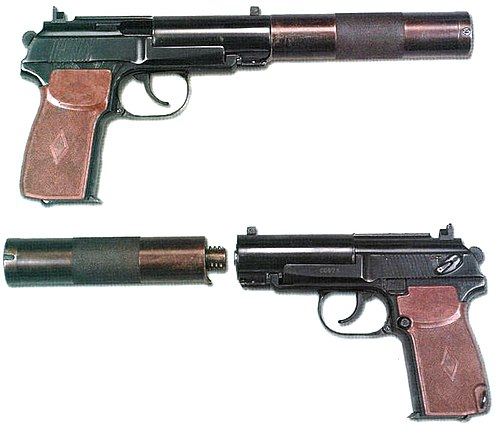
\includegraphics{../images/pistolety_i_pm/pb_1.jpg}
\caption{PB (6P9) --- tłumiony pistolet}
\end{figure}

\subsection{Opis}\label{opis-104}

PB (Пистолет Бесшумный --- Pistolet Bezgłośny, oznaczenie GRAU: 6P9) to
radziecki tłumiony pistolet kalibru 9×18 mm Makarov opracowany przez
A.A. Dyeewa na bazie PM i przyjęty do służby w 1967 roku dla KGB i GRU.
Wyróżnia się zintegrowanym układem tłumienia dźwięku podzielonym na dwa
elementy --- wewnętrzny tłumik w ramie (zastępuje część ramy) i
zewnętrzny tłumik przykręcany do lufy; całość przy złożonym tłumiku
zewnętrznym mieści się w standardowej kaburze. PB jest przeznaczony do
cichego eliminowania celów na bliskich odległościach (do 25 m) ---
stosowany przez wywiad wojskowy, KGB i siły specjalne w Afganistanie,
Czeczenii i operacjach specjalnych GRU.

\subsection{Dane techniczne}\label{dane-techniczne-104}

\begin{longtable}[]{@{}ll@{}}
\toprule\noalign{}
Parametr & Wartość \\
\midrule\noalign{}
\endhead
\bottomrule\noalign{}
\endlastfoot
Typ & Tłumiony pistolet samopowtarzalny \\
Kraj produkcji & ZSRR / Rosja \\
Rok wprowadzenia & 1967 \\
Kaliber & 9×18 mm Makarov \\
Długość (bez tłumika zewnętrznego) & 170 mm \\
Długość (z tłumikiem zewnętrznym) & 310 mm \\
Długość lufy & 105 mm \\
Masa (bez tłumika i magazynka) & 970 g \\
Pojemność magazynka & 8 nabojów \\
Prędkość wylotowa & 290 m/s (poddźwiękowa) \\
Skuteczny zasięg & 25--50 m \\
\end{longtable}

\subsection{Charakterystyczne cechy
rozpoznawcze}\label{charakterystyczne-cechy-rozpoznawcze-104}

\begin{quote}
Jak odróżnić PB od PM i pistoletów z tłumikami dokręcanymi:
\end{quote}

\begin{itemize}
\tightlist
\item
  \textbf{Widoczna ``szczelina'' w ramie z lewej strony --- wewnętrzny
  tłumik:} PB ma charakterystyczną podłużną szczelinę lub otwory w
  przedniej lewej części ramy --- to wloty wewnętrznego tłumika
  zintegrowanego z ramą; żaden standardowy PM nie ma otworów w ramie; ta
  cecha jest natychmiastowym identyfikatorem
\item
  \textbf{Zewnętrzny tłumik cylindryczny przykręcany z przodu:} z
  zewnętrznym tłumikiem PB ma charakterystyczną cylindryczną ``rurę''
  dłuższą niż lufa; tłumik PB jest stosunkowo krótki w porównaniu do
  wielu zachodnich tłumikowych pistoletów
\item
  \textbf{Bez tłumika zewnętrznego --- wizualnie bardzo podobny do PM:}
  PB bez zewnętrznego tłumika jest bardzo zbliżony wizualnie do PM;
  różnice to otwory w ramie i nieco dłuższa lufa; trudny do odróżnienia
  dla nieeżperta bez bliższego oglądania
\item
  \textbf{Poddźwiękowa prędkość wylotowa --- słyszalny tylko mechanizm:}
  pocisk 9×18 mm z PB leci z prędkością 290 m/s (poniżej prędkości
  dźwięku 340 m/s); jedynym słyszalnym dźwiękiem jest mechanizm zamkowy;
  z zewnątrz strzał brzmi jak ``klik'' z metalowego mechanizmu
\item
  \textbf{Magazynek 8-nabojowy --- identyczny z PM:} magazynek PB jest
  identyczny z PM (8 nabojów 9×18); odróżnienie PB od PM po magazynku
  jest niemożliwe
\item
  \textbf{Broń specjalna --- rzadkość poza jednostkami wywiadowczymi:}
  PB pojawia się prawie wyłącznie na fotografiach sił specjalnych i
  agentów wywiadu; widok tej broni sugeruje operację specjalną lub
  jednostkę Spetsnaz
\end{itemize}

\subsection{Ciekawostka}\label{ciekawostka-104}

\begin{quote}
PB był jedną z pierwszych broni użytych przez sowieckich ``cichych
likwidatorów'' w Afganistanie --- żołnierze Specnaz GRU przeznaczeni do
eliminowania mudżahedińskich dowódców nosili PB jako broń
``ostateczności''. Afgański konflikt ujawnił jednak słabość 9×18 mm ---
słaba siła zatrzymania na celach w grubych ubraniach zimowych. Dlatego w
Afganistanie Specnaz szybko przeszedł na VSS Wintorez (9×39 mm) do akcji
wymagających cichości i siły rażenia jednocześnie, a PB pozostał jako
``pistolet drugorzędny'' dla agentów wywiadu.
\end{quote}

\section{Pistolet PSM}\label{pistolet-psm}

\subsubsection{PSM Pistol \textbar{} ПСМ (Пистолет Самозарядный
Малогабаритный)}\label{psm-pistol-ux43fux441ux43c-ux43fux438ux441ux442ux43eux43bux435ux442-ux441ux430ux43cux43eux437ux430ux440ux44fux434ux43dux44bux439-ux43cux430ux43bux43eux433ux430ux431ux430ux440ux438ux442ux43dux44bux439}

\begin{center}\rule{0.5\linewidth}{0.5pt}\end{center}

\begin{figure}
\centering
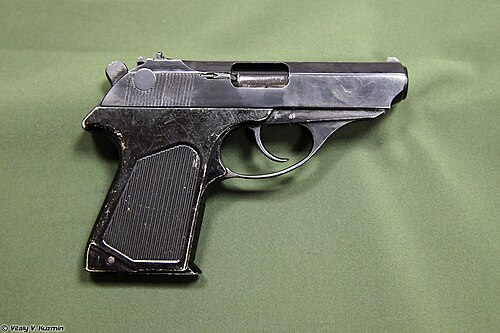
\includegraphics{../images/pistolety_i_pm/psm_1.jpg}
\caption{PSM --- ultrakompaktowy pistolet}
\end{figure}

\subsection{Opis}\label{opis-105}

PSM (Пистолет Самозарядный Малогабаритный --- Pistolet Samopowtarzalny
Małogabarytowy) to radziecki ultrakompaktowy pistolet kalibru 5,45×18 mm
MPts opracowany przez TsNIITochMash i przyjęty do służby w 1972 roku dla
KGB, oficerów wywiadu i oficerów sztabowych wymagających dyskretnej
broni osobistej. Charakteryzuje się wyjątkową płaskością --- PSM ma
zaledwie 17 mm grubości, co pozwala na noszenie pod marynarką bez
widocznej sylwetki. Nabój 5,45×18 mm ma wysoki współczynnik penetracji
--- przebija kamizelki balistyczne klasy I oraz szyby samochodowe;
pocisk jest bardzo lekki i szybki. PSM jest do dziś symbolem ``pistoletu
szpiega'' --- noszonego przez sowieckich i rosyjskich agentów wywiadu.

\subsection{Dane techniczne}\label{dane-techniczne-105}

\begin{longtable}[]{@{}ll@{}}
\toprule\noalign{}
Parametr & Wartość \\
\midrule\noalign{}
\endhead
\bottomrule\noalign{}
\endlastfoot
Typ & Ultrakompaktowy pistolet samopowtarzalny \\
Kraj produkcji & ZSRR / Rosja \\
Rok wprowadzenia & 1972 \\
Kaliber & 5,45×18 mm MPts \\
Długość & 155 mm \\
Szerokość & 17 mm \\
Długość lufy & 85 mm \\
Masa (bez magazynka) & 460 g \\
Pojemność magazynka & 8 nabojów \\
Prędkość wylotowa & 315 m/s \\
Skuteczny zasięg & 25 m \\
\end{longtable}

\subsection{Charakterystyczne cechy
rozpoznawcze}\label{charakterystyczne-cechy-rozpoznawcze-105}

\begin{quote}
Jak odróżnić PSM od PM i innych pistoletów kompaktowych:
\end{quote}

\begin{itemize}
\tightlist
\item
  \textbf{Wyjątkowo płaski profil --- tylko 17 mm grubości:} PSM jest
  niemal dwukrotnie cieńszy od PM (17 mm vs \textasciitilde30 mm); przy
  oglądaniu od przodu PSM wygląda jak ``kartka'' w porównaniu do PM; ta
  płaskość jest ikoniczną cechą wizualną PSM
\item
  \textbf{Mały kaliber --- cienka lufa, mały otwór wylotowy:} lufa PSM w
  kalibrze 5,45 mm ma wyraźnie mniejszą średnicę otworu niż lufa PM (9
  mm); przy bliskim oglądaniu lub na fotografii zbliżeniowej wyraźna
  różnica w kalibrze
\item
  \textbf{Prostokątny, ``tabliczkowy'' kształt --- bez żadnych
  zaokrągleń:} PSM ma charakterystyczny bardzo prostokątny, ``płaski
  tabliczkowy'' kształt bez wyraźnych krzywizn; PM jest zaokrąglony; PSM
  wygląda geometrycznie jak ``prostokąt z lufą''
\item
  \textbf{Minimalistyczne przyrządy celownicze --- prawie bez
  celownika:} PSM ma bardzo małe, prawie niewidoczne przyrządy
  celownicze; to broń na bliski dystans (25 m), gdzie celownik nie jest
  krytyczny; przy oglądaniu z góry widać mikroskopijny celownik i muszkę
\item
  \textbf{Brak zewnętrznego kurka (hammer-less lub internal):} PSM nie
  ma widocznego zewnętrznego kurka; profil tylnej części zamka jest
  gładki --- co dodatkowo zmniejsza grubość i zapobiega zaczepieniu przy
  dobywaniu; PM ma wyraźny kurek z tyłu
\item
  \textbf{Bardzo lekki --- 460 g --- ``prawie nieważki'':} PSM waży 460
  g bez magazynka; PM waży 730 g; różnica masy jest wyczuwalna przy
  trzymaniu; PSM ``znika'' w kieszeni marynarki
\end{itemize}

\subsection{Ciekawostka}\label{ciekawostka-105}

\begin{quote}
PSM był przez lata pistoletem, którego zachodni agenci wywiadu bali się
najbardziej --- nie ze względu na siłę, ale na przenikliwość naboju
5,45×18 mm. CIA odkryła, że PSM przebija ówczesne kamizelki kevlarowe
klasy I, które chroniły przed nabojami pistoletowymi. Przez lata
70.--80. agenci chronieni przez CIA i FBI nosili kamizelki
nieprzebijalne przez pistolety --- ale niechroniące przed PSM. Sowieccy
oficerowie wywiadu nosili PSM właśnie po to, by mieć ``przewagę
przenikania'' nad potencjalnymi zachodnimi ochroniarzami.
\end{quote}

\section{Pistolet MP-443 Grach}\label{pistolet-mp-443-grach}

\subsubsection{MP-443 Grach (PYa) Pistol \textbar{} МП-443 «Грач»
(ПЯ)}\label{mp-443-grach-pya-pistol-ux43cux43f-443-ux433ux440ux430ux447-ux43fux44f}

\begin{center}\rule{0.5\linewidth}{0.5pt}\end{center}

\begin{figure}
\centering
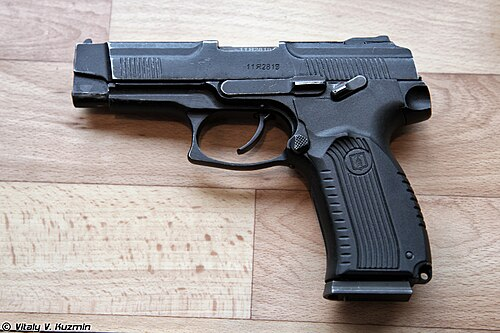
\includegraphics{../images/pistolety_i_pm/mp-443_1.jpg}
\caption{MP-443 Grach --- pistolet 9×19 mm}
\end{figure}

\subsection{Opis}\label{opis-106}

MP-443 Grach (Грач --- Gawron), oficjalnie PYa (Pistolet Yarygina), to
rosyjski pistolet samopowtarzalny kalibru 9×19 mm Parabellum opracowany
przez Władimira Yarygina i przyjęty do służby w 2003 roku jako oficjalny
następnik PM. Standardowy pistolet armii rosyjskiej i policji nowej
generacji --- używa NATO-wskiego kalibru 9×19 mm, co jest istotną zmianą
od 9×18 mm PM. Duży magazynek 17-nabojowy, podwójne działanie spustu
(DA/SA), szyna Picatinny pod lufą i ergonomiczny polymer-frame chwyt
sprawiają, że MP-443 jest nowoczesną bronią policyjną i wojskową klasy
XXI wieku. Był wolno wdrażany ze względu na problemy z jakością
produkcji w latach 2000.; od 2010 roku dostawy są stabilne.

\subsection{Dane techniczne}\label{dane-techniczne-106}

\begin{longtable}[]{@{}ll@{}}
\toprule\noalign{}
Parametr & Wartość \\
\midrule\noalign{}
\endhead
\bottomrule\noalign{}
\endlastfoot
Typ & Pistolet samopowtarzalny \\
Kraj produkcji & Rosja \\
Rok wprowadzenia & 2003 \\
Kaliber & 9×19 mm Parabellum \\
Długość & 198 mm \\
Długość lufy & 112 mm \\
Masa (bez magazynka) & 950 g \\
Pojemność magazynka & 17 nabojów \\
Prędkość wylotowa & 465 m/s \\
Skuteczny zasięg & 50 m \\
\end{longtable}

\subsection{Charakterystyczne cechy
rozpoznawcze}\label{charakterystyczne-cechy-rozpoznawcze-106}

\begin{quote}
Jak odróżnić MP-443 od PM i zachodnich pistoletów:
\end{quote}

\begin{itemize}
\tightlist
\item
  \textbf{Wyraźnie większy i masywniejszy od PM --- ``nowoczesny
  policyjny'' wygląd:} MP-443 jest wyraźnie większy od PM; szerszy chwyt
  (dwurzędowy magazynek 17 nabojów), dłuższa lufa; przy porównaniu PM
  wygląda jak ``mały, stary pistolet'' obok nowoczesnego MP-443
\item
  \textbf{Szyna Picatinny pod lufą --- charakterystyczny ``ząb'' pod
  rurą:} MP-443 ma wyraźną szynę taktyczną pod lufą do latarki lub
  lasera; PM nie ma szyny; ta szyna jest jedną z pierwszych różnic
  widocznych od razu
\item
  \textbf{Szeroki, wysoki chwyt na dwurzędowy magazynek 17 nabojów:}
  chwyt MP-443 jest wyraźnie szerszy i wyższy od chwytu PM (8 nabojów);
  przy trzymaniu w dłoni widoczna jest wyraźna różnica w ``objętości''
  uchwytu
\item
  \textbf{Czarny polymer lub metal --- nowoczesna ergonomia:} MP-443 ma
  czarny polimerowy lub stalowy chwyt z wyraźnymi ryflowaniami
  antypoślizgowymi; PM ma gładkie okładziny bakelitowe lub gumowe;
  estetyka MP-443 jest wyraźnie nowoczesna
\item
  \textbf{Zewnętrzny kurek z tyłu slajdu --- jak PM:} MP-443 zachowuje
  zewnętrzny kurek z tyłu zamka (jak PM); to odróżnia go od pistoletów
  ``hammerless'' (bez kurka zewnętrznego); kurek MP-443 jest mniejszy i
  nowocześniej ukształtowany niż kurek PM
\item
  \textbf{Dźwignia bezpiecznika po lewej stronie ramy --- jak PM:}
  MP-443 ma bezpiecznik po lewej stronie ramy; PM też ma bezpiecznik w
  tym miejscu; to cecha wspólna rosyjskich pistoletów odróżniająca od
  wielu zachodnich konstrukcji
\end{itemize}

\subsection{Ciekawostka}\label{ciekawostka-106}

\begin{quote}
MP-443 Grach miał jedną z najdłuższych i najbardziej problematycznych
dróg do służby spośród nowoczesnych rosyjskich broni. Oficjalnie
przyjęty w 2003 roku, przez kolejne siedem lat borykał się z problemami
produkcyjnymi --- pęknięcia ramy, zawodność zasilania. Żołnierze
rosyjscy z pierwszych dostaw żartowali, że ``Grach lata gorzej niż stary
PM''. Sytuacja poprawiła się około 2010 roku, ale PM wciąż służy jako
broń zapasowa i w policji ze względu na olbrzymie zapasy magazynowe. W
2022 roku na Ukrainie strzelcy obu stron identyfikują pistolet rosyjski
po tym, czy nosi PM (starszy, rezerwysta) czy MP-443 (młodszy, aktywna
służba).
\end{quote}

\section{Pistolet GSz-18}\label{pistolet-gsz-18}

\subsubsection{GSh-18 Pistol \textbar{}
ГШ-18}\label{gsh-18-pistol-ux433ux448-18}

\begin{center}\rule{0.5\linewidth}{0.5pt}\end{center}

\begin{figure}
\centering
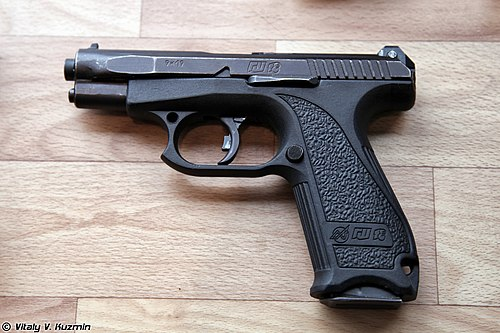
\includegraphics{../images/pistolety_i_pm/gsh-18_1.jpg}
\caption{GSz-18 --- pistolet 9×19 mm}
\end{figure}

\subsection{Opis}\label{opis-107}

GSz-18 (ГШ-18 --- Griaziew-Szipunow, 18 nabojów) to rosyjski pistolet
samopowtarzalny kalibru 9×19 mm opracowany przez KBP (Griaziew i
Szipunow) w Tule i przyjęty do służby w 2000 roku. Wyróżnia się
wyjątkowo lekką polimerową ramą i obrotowym zamkiem (locked breech
rotating barrel) --- oryginalnym mechanizmem, który redukuje masę i
odrzut. Dedykowana amunicja 9×19 mm PBP (7N31) ma rdzeń ze stali
narzędziowej i przebija kamizelki balistyczne klasy III A na 10 m --- co
czyni GSz-18 jednym z najbardziej penetracyjnych pistoletów na świecie.
Stosowany przez FSB, policję specjalną i wybrane jednostki wojskowe;
konkuruje z MP-443 o rolę standardowego pistoletu.

\subsection{Dane techniczne}\label{dane-techniczne-107}

\begin{longtable}[]{@{}ll@{}}
\toprule\noalign{}
Parametr & Wartość \\
\midrule\noalign{}
\endhead
\bottomrule\noalign{}
\endlastfoot
Typ & Pistolet samopowtarzalny \\
Kraj produkcji & Rosja \\
Rok wprowadzenia & 2000 \\
Kaliber & 9×19 mm Parabellum / 9×19 mm PBP \\
Długość & 184 mm \\
Długość lufy & 103 mm \\
Masa (bez magazynka) & 590 g \\
Pojemność magazynka & 18 nabojów \\
Prędkość wylotowa & 600 m/s (7N31 PBP) \\
Skuteczny zasięg & 50 m \\
\end{longtable}

\subsection{Charakterystyczne cechy
rozpoznawcze}\label{charakterystyczne-cechy-rozpoznawcze-107}

\begin{quote}
Jak odróżnić GSz-18 od MP-443 i PM:
\end{quote}

\begin{itemize}
\tightlist
\item
  \textbf{Wyjątkowo lekki --- 590 g --- najlżejszy wśród rosyjskich
  pistoletów służbowych:} GSz-18 waży zaledwie 590 g bez magazynka; PM
  waży 730 g, MP-443 --- 950 g; ta lekkość jest odczuwalna w ręce i
  widoczna w sposobie trzymania przez strzelca
\item
  \textbf{Polimerowa rama z bardzo widoczną szyną Picatinny:} GSz-18 ma
  wyraźną szynę pod lufą jak MP-443; ale cała rama jest wyraźnie
  bardziej ``plastikowa'' i lekka; połączenie dużej szyny i lekkiego
  wyglądu jest charakterystyczne
\item
  \textbf{Charakterystyczny kształt ``trójkątnego'' chwytu z tylnym
  wycięciem:} chwyt GSz-18 ma charakterystyczny kształt ze specjalnym
  wycięciem w tylnej części ramy dla kciuka drugiej ręki; kształt jest
  geometrycznie unikalny wśród rosyjskich pistoletów
\item
  \textbf{Brak zewnętrznego kurka --- ``hammerless'' striker-fired:}
  GSz-18 nie ma widocznego zewnętrznego kurka; tylna część slajdu jest
  gładka; to odróżnia od PM i MP-443 (oba z kurkiem zewnętrznym); wygląd
  ``bez kurka'' jest charakterystyczny
\item
  \textbf{Magazynek 18-nabojowy --- wyraźnie duże pudełko magazynka:}
  magazynek na 18 nabojów jest jednym z największych w klasie rosyjskich
  pistoletów; chwyt jest odpowiednio szeroki --- widoczna przy magazynku
  o dużej pojemności szerokość chwytu
\item
  \textbf{Rzadziej spotykany niż PM i MP-443 --- broń ``elitarna'':}
  GSz-18 jest mniej powszechny niż PM; jego widok sugeruje FSB, policję
  specjalną lub oficera wywiadu; w regularnej armii rzadki
\end{itemize}

\subsection{Ciekawostka}\label{ciekawostka-107}

\begin{quote}
GSz-18 z amunicją 7N31 PBP jest jednym z niewielu pistoletów na świecie
zdolnych do przebicia standardowych kamizelek balistycznych NATO klasy
IIIA na odległość 10 metrów. Eksperymenty wykazały, że 7N31 przebija 8
mm stali budowlanej z 10 m --- co jest wynikiem niespotykawym dla naboju
pistoletowego 9 mm. Zachodni eksperci byli zaskoczeni, bo NATO przez
lata zakładało, że kamizelki IIIA chronią przed wszystkimi pistoletami.
GSz-18 zademonstrował, że ``standardowa ochrona'' nie jest standardem
uniwersalnym.
\end{quote}

\section{Pistolet SR-1 Wektor (SPS)}\label{pistolet-sr-1-wektor-sps}

\subsubsection{SR-1 Vektor (SPS) Pistol \textbar{} СР-1 «Вектор»
(СПС)}\label{sr-1-vektor-sps-pistol-ux441ux440-1-ux432ux435ux43aux442ux43eux440-ux441ux43fux441}

\begin{center}\rule{0.5\linewidth}{0.5pt}\end{center}

\begin{figure}
\centering
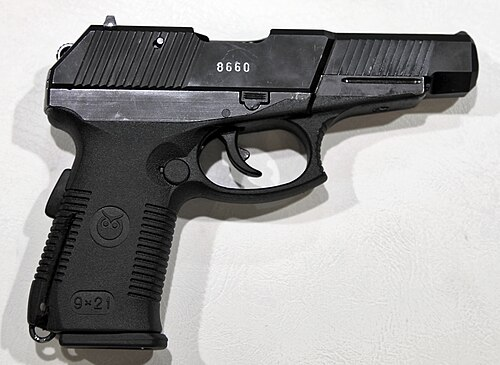
\includegraphics{../images/pistolety_i_pm/sr-1_1.jpg}
\caption{SR-1 Wektor --- pistolet wysokopenetracyjny}
\end{figure}

\subsection{Opis}\label{opis-108}

SR-1 Wektor (Вектор --- Wektor), oficjalnie SPS (Самозарядный Пистолет
Сердюкова --- Samopowtarzalny Pistolet Sierdiukowa), to rosyjski
pistolet kalibru 9×21 mm SP-10 opracowany przez TsNIITochMash i przyjęty
do służby w 1996 roku dla FSB i GRU. Wyróżnia się dedykowaną amunicją
9×21 mm SP-10, której stal-rdzeniowy pocisk przebija kamizelki IIIA z 50
m i 8 mm płyty stalowe; jest to jeden z najbardziej penetracyjnych
pistoletów na świecie. SR-1 jest bronią stricte specjalną --- dla
operatorów wymagających pistoletu przebijającego opancerzone cele.
Mechanizm zamkowy z obrotową lufą (podobnie jak GSz-18) redukuje odrzut.
Stosowany przez FSB, GRU i sił specjalnych.

\subsection{Dane techniczne}\label{dane-techniczne-108}

\begin{longtable}[]{@{}ll@{}}
\toprule\noalign{}
Parametr & Wartość \\
\midrule\noalign{}
\endhead
\bottomrule\noalign{}
\endlastfoot
Typ & Pistolet samopowtarzalny wysokopenetracyjny \\
Kraj produkcji & Rosja \\
Rok wprowadzenia & 1996 \\
Kaliber & 9×21 mm SP-10 \\
Długość & 200 mm \\
Długość lufy & 120 mm \\
Masa (bez magazynka) & 900 g \\
Pojemność magazynka & 18 nabojów \\
Prędkość wylotowa & 400 m/s (SP-10) \\
Skuteczny zasięg & 50 m \\
\end{longtable}

\subsection{Charakterystyczne cechy
rozpoznawcze}\label{charakterystyczne-cechy-rozpoznawcze-108}

\begin{quote}
Jak odróżnić SR-1 od MP-443 i GSz-18:
\end{quote}

\begin{itemize}
\tightlist
\item
  \textbf{Wyraźnie masywniejszy i grubszy od MP-443 i GSz-18:} SR-1 jest
  większy i cięższy od obydwu --- wyraźna ``mięsistość'' broni; szeroki
  chwyt na magazynek 18-nabojowy; ogólna bryła jest solidna i duża jak
  na pistolet
\item
  \textbf{Widoczna szyna pod lufą i nowoczesna ergonomia:} SR-1 ma szynę
  Picatinny pod lufą; ergonomia jest nowoczesna z wyraźnym trójkątnym
  profilem uchwytu; wygląd zbliżony do MP-443, ale masywniejszy
\item
  \textbf{Charakterystyczny zewnętrzny kurek zaokrąglony (bobbed
  hammer):} SR-1 ma zewnętrzny kurek, ale jest ukryty i zaokrąglony; nie
  sterczy tak widocznie jak kurek PM; pośredni między zewnętrznym a
  wewnętrznym
\item
  \textbf{Niestandardowy kaliber 9×21 mm --- amunicja niekompatybilna z
  innymi:} SR-1 używa unikalnej amunicji 9×21 mm SP-10 niepasującej do
  żadnego innego pistoletu; przy obserwacji załadowania naboje są
  wyraźnie dłuższe od standardowych 9×19 mm Parabellum; ta ``obca''
  amunicja identyfikuje SR-1
\item
  \textbf{Rzadki --- widoczny głównie u FSB i specnazowców:} SR-1 jest
  bronią elitarną i rzadką; jego widok na fotografii sugeruje operatora
  specjalnego FSB lub GRU; regularna policja i wojsko używają PM lub
  MP-443
\item
  \textbf{Złożona gumowa lub polimerowa okładzina chwytu:} okładziny
  chwytu SR-1 są ergonomiczne z gumowymi wstawkami antypoślizgowymi;
  nowoczesny wygląd odróżnia od prostych okładzin PM
\end{itemize}

\subsection{Ciekawostka}\label{ciekawostka-108}

\begin{quote}
SR-1 Wektor był pierwszym rosyjskim pistoletem zaprojektowanym po zimnej
wojnie z eksplicytnym wymaganiem ``przebij kamizelkę IIIA''. Projektanci
TsNIITochMash mieli do dyspozycji analizy operacji FSB z lat 90., gdzie
okazało się, że czeczeńscy bojownicy i gangsterzy nosili zachodnie
kamizelki balistyczne --- i standardowy PM był bezsilny. SR-1 z amunicją
SP-10 był odpowiedzią: pistolet, który można nosić dyskretnie, ale który
przebija to, czego PM nie przebija. Zachodnie analizy po pierwszym
opisaniu SR-1 w publicznych źródłach w 2000 roku spowodowały przegląd
standardów certyfikacji kamizelek NATO.
\end{quote}

\section{Pistolet maszynowy OTs-33
Piernacz}\label{pistolet-maszynowy-ots-33-piernacz}

\subsubsection{OTs-33 Pernach Machine Pistol \textbar{} ОЦ-33
«Пернач»}\label{ots-33-pernach-machine-pistol-ux43eux446-33-ux43fux435ux440ux43dux430ux447}

\begin{center}\rule{0.5\linewidth}{0.5pt}\end{center}

\begin{figure}
\centering
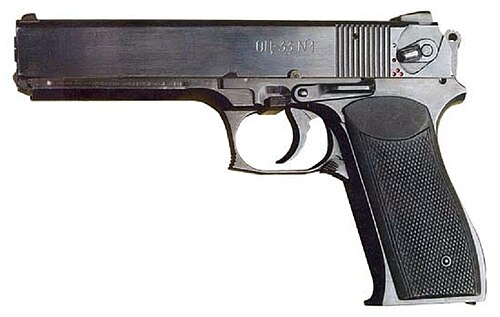
\includegraphics{../images/pistolety_i_pm/ots-33_1.jpg}
\caption{OTs-33 Piernacz --- pistolet maszynowy}
\end{figure}

\subsection{Opis}\label{opis-109}

OTs-33 Piernacz (Пернач --- historyczna buława policyjna) to rosyjski
pistolet maszynowy kalibru 9×18 mm Makarov opracowany przez KBP w Tule i
przyjęty do służby w 1999 roku dla policji specjalnej i sił szybkiego
reagowania. Wyróżnia się kompaktową budową z automatycznym ogniem (850
strz./min) i magazynkiem 27-nabojowym --- przy rozmiarach zaledwie
nieznacznie większych od PM. Odpinaną kolba szkieletowa (do montażu z
tyłu) pozwala na celny ogień automatyczny. OTs-33 jest bronią
przeznaczoną dla operatorów policyjnych i jednostek antyterrorystycznych
wymagających kompaktowej broni z możliwością ognia automatycznego;
stosowany przez OMON, FSB i rosyjskie jednostki specjalne.

\subsection{Dane techniczne}\label{dane-techniczne-109}

\begin{longtable}[]{@{}ll@{}}
\toprule\noalign{}
Parametr & Wartość \\
\midrule\noalign{}
\endhead
\bottomrule\noalign{}
\endlastfoot
Typ & Pistolet maszynowy / pistolet automatyczny \\
Kraj produkcji & Rosja \\
Rok wprowadzenia & 1999 \\
Kaliber & 9×18 mm Makarov \\
Długość (bez kolby) & 205 mm \\
Długość (z kolbą złożoną) & 360 mm \\
Długość lufy & 130 mm \\
Masa (bez magazynka) & 1 050 g \\
Pojemność magazynka & 27 nabojów \\
Szybkostrzelność & 850 strz./min (auto) \\
Skuteczny zasięg & 50 m (pistolet) / 100 m (z kolbą) \\
\end{longtable}

\subsection{Charakterystyczne cechy
rozpoznawcze}\label{charakterystyczne-cechy-rozpoznawcze-109}

\begin{quote}
Jak odróżnić OTs-33 od APS i PM:
\end{quote}

\begin{itemize}
\tightlist
\item
  \textbf{Wyraźnie większy magazynek --- 27 nabojów sterczy poniżej
  chwytu:} magazynek OTs-33 na 27 nabojów jest długi i wyraźnie sterczy
  poniżej dolnej krawędzi chwytu; PM ma krótki magazynek 8-nabojowy; ta
  długość magazynka jest widoczna
\item
  \textbf{Dwa przełączniki trybu ognia --- widoczne po lewej stronie:}
  OTs-33 ma selektor trybu ognia (semi/auto/bezpiecznik) po lewej
  stronie; APS też ma selektor; PM nie ma; widoczna dźwignia selektora
  identyfikuje broń z możliwością ognia automatycznego
\item
  \textbf{Kolba szkieletowa odcinana --- nowocześniejsza od kabury-kolby
  APS:} OTs-33 ma nowoczesną metalową kolbę szkieletową (nie kaburę jak
  APS); kolba ma inny kształt od kaburo-kolby APS; bardziej
  ``taktyczny'' wygląd
\item
  \textbf{Nieco krótszy od APS --- kompaktowszy dla użycia policyjnego:}
  OTs-33 (205 mm bez kolby) jest nieco krótszy od APS (225 mm);
  proporcje są zbliżone, ale OTs-33 jest bardziej zwarty; oba są
  wyraźnie większe od PM
\item
  \textbf{Charakterystyczna ``podwójna'' linia z boku zamka:} zamek
  OTs-33 ma widoczne linie ryflowania do naciągania zarówno z przodu jak
  i z tyłu; ta ``podwójna'' strefa chwytu do naciągania jest
  nowocześ­niejsza i bardziej rozbudowana niż w APS
\item
  \textbf{Broń policyjna --- widoczna głównie u OMON i FSB:} OTs-33
  pojawia się głównie na fotografiach jednostek policyjnych i
  antyterrorystycznych, rzadko w regularnym wojsku; ten kontekst użycia
  jest sam w sobie identyfikatorem
\end{itemize}

\subsection{Ciekawostka}\label{ciekawostka-109}

\begin{quote}
Nazwa ``Piernacz'' pochodzi od historycznej polsko-rosyjskiej broni
ceremonialnej --- buławy z piórami (piernacz), symbolizującej władzę
dowódcy. Projektanci KBP wybrali tę nazwę żartobliwie sugerując, że
OTs-33 jest ``buławą nowoczesnego dowódcy policji'' --- kompaktową
bronią godną oficera, a nie tylko strażnika. Ironia polega na tym, że
Piernacz jest jedną z rzadszych broni w rosyjskim arsenale policyjnym
--- jego wysoka szybkostrzelność (850 strz./min) i kaliber 9×18 mm są
dobre do walki w pomieszczeniach, ale ograniczone zasięgiem; OMON
preferuje karabiny szturmowe do zewnętrznych operacji.
\end{quote}

\section{Pistolet maszynowy OTs-23
Drotik}\label{pistolet-maszynowy-ots-23-drotik}

\subsubsection{OTs-23 Drotik Machine Pistol \textbar{} ОЦ-23
«Дротик»}\label{ots-23-drotik-machine-pistol-ux43eux446-23-ux434ux440ux43eux442ux438ux43a}

\begin{center}\rule{0.5\linewidth}{0.5pt}\end{center}

\begin{figure}
\centering
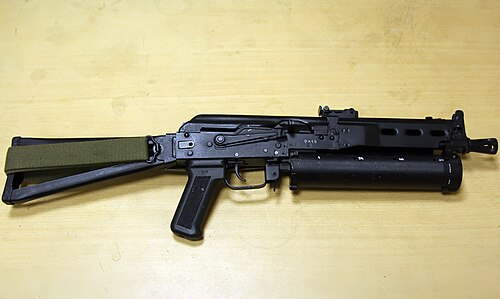
\includegraphics{../images/pistolety_i_pm/ots-23_1.jpg}
\caption{OTs-23 Drotik --- pistolet maszynowy}
\end{figure}

\subsection{Opis}\label{opis-110}

OTs-23 Drotik (Дротик --- Oszczep, rzutka) to rosyjski automatyczny
pistolet maszynowy kalibru 5,45×18 mm MPts opracowany przez KBP w Tule w
latach 90. dla policji i sił specjalnych. Wyróżnia się trójstrzałową
serią z opóźnieniem --- mechanizm strzelający oddaje trzy naboje przed
skokiem zamka, co redukuje rozrzut serii. Kaliber 5,45×18 mm to ten sam
co PSM --- pocisk przenika kamizelki klasy I-II. Bardzo kompaktowa broń
(długość 305 mm bez kolby) przeznaczona dla oficerów ochrony,
policjantów w służbie cywilnej i agentów wywiadu. Nie była szeroko
wdrażana ze względu na ograniczoną dostępność amunicji 5,45×18 mm;
stosowana przez FSO (ochrona Kremla) i wybrane oddziały FSB.

\subsection{Dane techniczne}\label{dane-techniczne-110}

\begin{longtable}[]{@{}ll@{}}
\toprule\noalign{}
Parametr & Wartość \\
\midrule\noalign{}
\endhead
\bottomrule\noalign{}
\endlastfoot
Typ & Pistolet maszynowy / pistolet automatyczny \\
Kraj produkcji & Rosja \\
Rok wprowadzenia & ok. 1994 \\
Kaliber & 5,45×18 mm MPts \\
Długość (bez kolby) & 305 mm \\
Długość (z kolbą złożoną) & 535 mm \\
Długość lufy & 135 mm \\
Masa (bez magazynka) & 1 100 g \\
Pojemność magazynka & 24 nabojów \\
Szybkostrzelność & 1 700 strz./min (seryjnie) \\
Skuteczny zasięg & 50 m \\
\end{longtable}

\subsection{Charakterystyczne cechy
rozpoznawcze}\label{charakterystyczne-cechy-rozpoznawcze-110}

\begin{quote}
Jak odróżnić OTs-23 od PP-2000 i PM:
\end{quote}

\begin{itemize}
\tightlist
\item
  \textbf{Mały kaliber --- lufa wyraźnie cieńsza niż 9 mm pistolety:}
  OTs-23 w kalibrze 5,45 mm ma wyraźnie cieńszą lufę niż pistolety 9 mm
  (PM, MP-443); przy oglądaniu z przodu otwór lufy jest wyraźnie
  mniejszy
\item
  \textbf{Składana kolba druciana --- jak Kedr lub UZI:} OTs-23 ma
  metalową drucianą kolbę składaną do tyłu lub na bok; charakterystyczna
  ``druciana kratownica'' jako kolba jest zbliżona do Kedr i UZI
\item
  \textbf{Długi magazynek 24-nabojowy wyraźnie sterczący z chwytu:}
  magazynek 24 nabojów na kaliber 5,45×18 mm jest długi (naboje są
  wąskie więc magazynek jest smukły ale długi); sterczy wyraźnie poniżej
  chwytu; PSM (ten sam kaliber) ma tylko 8 nabojów
\item
  \textbf{Rzadkość --- broń prawie nieznana poza Rosją:} OTs-23 Drotik
  jest jedną z rzadszych rosyjskich broni specjalnych; jego widok
  sugeruje specjalistyczną kolekcję lub bardzo wąskie zastosowanie
  FSO/FSB; przy pokazywaniu broni ``co to jest?'' jest częstą reakcją
\item
  \textbf{Selektor trybu ognia z możliwością serii 3-nabojowych:} OTs-23
  ma selektor z trybem serii 3-nabojowych --- charakterystyczna
  trójpozycyjna dźwignia; mniej pistoletów ma serię 3-nabojową jako
  opcję
\item
  \textbf{Mała, kompaktowa bryła bez szyny taktycznej:} OTs-23 jest
  prosty i kompaktowy --- bez szyny Picatinny (starszy projekt); wygląd
  ``prosty wojskowy'' bez nowoczesnych dodatków
\end{itemize}

\subsection{Ciekawostka}\label{ciekawostka-110}

\begin{quote}
OTs-23 Drotik był projektowany jako alternatywa dla PSM dla oficerów
wymagających większej pojemności magazynka i możliwości ognia
automatycznego --- ale w tym samym kalibrze 5,45×18 mm przenikającym
kamizelki. Niestety, kaliber 5,45×18 mm jest produkowany w ograniczonych
ilościach i dostępny głównie dla wojska; to spowodowało, że OTs-23 nigdy
nie był masowo wdrożony. Ironicznie, FSO (ochrona Kremla), która jest
jednym z głównych użytkowników Drotika, ma priorytetowy dostęp do
amunicji 5,45×18 mm --- bo chroni najważniejsze osoby w Rosji i musi
mieć broń zdolną do penetracji kamizelek ewentualnych zamachowców.
\end{quote}

\section{Pistolet maszynowy PP-91
Kedr}\label{pistolet-maszynowy-pp-91-kedr}

\subsubsection{PP-91 Kedr Submachine Gun \textbar{} ПП-91
«Кедр»}\label{pp-91-kedr-submachine-gun-ux43fux43f-91-ux43aux435ux434ux440}

\begin{center}\rule{0.5\linewidth}{0.5pt}\end{center}

\begin{figure}
\centering
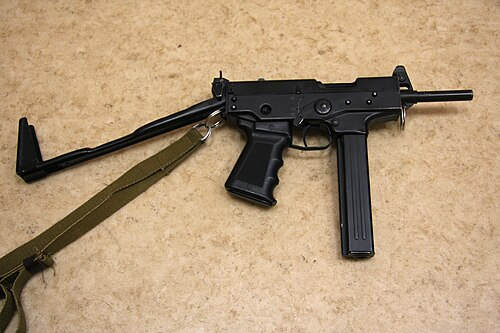
\includegraphics{../images/pistolety_i_pm/pp-91_1.jpg}
\caption{PP-91 Kedr --- pistolet maszynowy}
\end{figure}

\subsection{Opis}\label{opis-111}

PP-91 Kedr (Кедр --- Cedr syberyjski) to rosyjski pistolet maszynowy
kalibru 9×18 mm Makarov opracowany przez Jewgienija Dragonowa (syna
konstruktora SVD) i przyjęty do służby w 1994 roku dla policji i sił
specjalnych. Jest bardzo kompaktową bronią --- z kolbą złożoną mieści
się w kieszeni lub plecaku; przeznaczona dla ochroniarzy, policjantów w
terenie zabudowanym i obsługi pojazdów. Szybkostrzelność 1000 strz./min
i magazynek 20--30 nabojów dają dużą gęstość ognia na bliskich
odległościach (do 50 m). Kedr jest popularny wśród rosyjskich
policjantów i prywatnych firm ochrony. Wersja z tłumikiem to PP-91-01
Kedr-B.

\subsection{Dane techniczne}\label{dane-techniczne-111}

\begin{longtable}[]{@{}ll@{}}
\toprule\noalign{}
Parametr & Wartość \\
\midrule\noalign{}
\endhead
\bottomrule\noalign{}
\endlastfoot
Typ & Pistolet maszynowy (SMG) \\
Kraj produkcji & Rosja \\
Rok wprowadzenia & 1994 \\
Kaliber & 9×18 mm Makarov \\
Długość (kolba złożona) & 305 mm \\
Długość (kolba rozłożona) & 530 mm \\
Długość lufy & 120 mm \\
Masa (bez magazynka) & 1 540 g \\
Pojemność magazynka & 20 lub 30 nabojów \\
Szybkostrzelność & 1 000 strz./min \\
Skuteczny zasięg & 50 m \\
\end{longtable}

\subsection{Charakterystyczne cechy
rozpoznawcze}\label{charakterystyczne-cechy-rozpoznawcze-111}

\begin{quote}
Jak odróżnić PP-91 Kedr od PM i APS:
\end{quote}

\begin{itemize}
\tightlist
\item
  \textbf{Wyraźnie ``pistolet maszynowy'' --- dłuższy od pistoletu,
  krótszy od karabinu:} Kedr ma wyraźny ``pośredni'' rozmiar między
  pistoletem a karabinem szturmowym; z kolbą rozłożoną ma 530 mm --- jak
  AKS-74U; z kolbą złożoną --- 305 mm, jak duży pistolet
\item
  \textbf{Metalowa składana kolba szkieletowa --- charakterystyczna
  ``kratownica'':} Kedr ma typową składaną metalową kolbę szkieletową
  (drucianą kratownicę) jak wiele pistolety maszynowych z lat 90.; w
  złożeniu leży wzdłuż prawej strony broni
\item
  \textbf{Duży magazynek 20--30 nabojów sterczący z dołu chwytu:}
  magazynek Kedr jest wyraźnie dłuższy od magazynka PM; sterczy dość
  daleko poniżej chwytu; widoczna przy pierwszym spojrzeniu ``długa
  skrzynka'' pod pistoletem
\item
  \textbf{Szybkostrzelność 1000 strz./min --- seria brzmi inaczej niż
  AK:} Kedr strzela wyraźnie szybciej niż AK-74 (600 strz./min); przy
  oglądaniu serii na nagraniu rhythmiczny dźwięk jest wyraźnie szybszy
\item
  \textbf{Brak lufy wystającej z łoża --- lufa jest wewnątrz:} lufa Kedr
  jest ukryta w łożu prawie do wylotu; proporcje są ``kompaktowe'' ---
  brak długiej lufy odstającej jak w karabinach szturmowych
\item
  \textbf{Stosowany przez policję w cywilnym otoczeniu --- widoczny na
  zdjęciach funkcjonariuszy:} Kedr pojawia się głównie u rosyjskich
  policjantów, strażników i ochroniarzy; nie jest typową bronią
  wojskową; ten kontekst jest identyfikatorem
\end{itemize}

\subsection{Ciekawostka}\label{ciekawostka-111}

\begin{quote}
PP-91 Kedr zyskał sławę po tym, jak stał się standardowym uzbrojeniem
rosyjskich ochroniarzy VIP i policji ochrony osobistej w burzliwych
latach 90. W epoce rosyjskich ``wojen gangsterskich'' (1991--2000) firma
ochroniarska z Kedrem była symbolem ``poważnej ochrony''. Sam Kedr był
projektowany z myślą o tym właśnie zastosowaniu --- kompaktowy, silny
ogień w wąskich korytarzach i windach. Paradoksalnie, wersja cywilna
(semi-auto) sprzedawana była jako broń samoobronowa dla prywatnych
obywateli --- jeden z nielicznych przypadków, gdy broń wojskowa trafiła
na rynek cywilny w Rosji.
\end{quote}

\section{Pistolet maszynowy PP-2000}\label{pistolet-maszynowy-pp-2000}

\subsubsection{PP-2000 Submachine Gun \textbar{}
ПП-2000}\label{pp-2000-submachine-gun-ux43fux43f-2000}

\begin{center}\rule{0.5\linewidth}{0.5pt}\end{center}

\begin{figure}
\centering
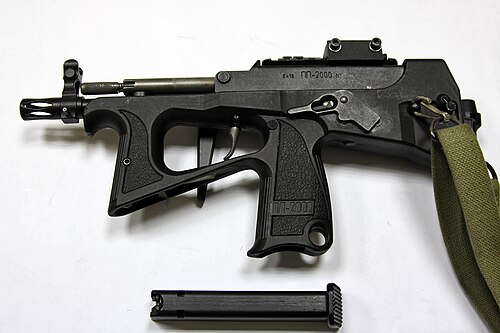
\includegraphics{../images/pistolety_i_pm/pp-2000_1.jpg}
\caption{PP-2000 --- pistolet maszynowy}
\end{figure}

\subsection{Opis}\label{opis-112}

PP-2000 to rosyjski pistolet maszynowy kalibru 9×19 mm Parabellum
opracowany przez KBP w Tule i przyjęty do służby w 2006 roku dla FSB,
policji i sił specjalnych. Wyróżnia się wyjątkową kompaktowością przy
kalibru 9×19 mm --- mniejszy od PP-91 Kedr przy używaniu mocniejszego
naboju NATO. Może używać standardowych magazynków 9×19 mm i specjalnych
nabojów API z rdzeniem wolframowym (7N31) do penetracji kamizelek IIIA.
Kolba ze złożonego magazynka 44-nabojowego (tylna kolba z dodatkowym
magazynkiem) jest unikalną cechą. Stosowany przez policję kryminalną,
FSB i ochronę VIP; pojawił się na Ukrainie.

\subsection{Dane techniczne}\label{dane-techniczne-112}

\begin{longtable}[]{@{}ll@{}}
\toprule\noalign{}
Parametr & Wartość \\
\midrule\noalign{}
\endhead
\bottomrule\noalign{}
\endlastfoot
Typ & Pistolet maszynowy \\
Kraj produkcji & Rosja \\
Rok wprowadzenia & 2006 \\
Kaliber & 9×19 mm Parabellum \\
Długość (bez kolby) & 340 mm \\
Długość (z kolbą/mag. 44 nab.) & 582 mm \\
Długość lufy & 179 mm \\
Masa (bez magazynka) & 1 400 g \\
Pojemność magazynka & 20 lub 44 nabojów \\
Szybkostrzelność & 600--800 strz./min \\
Skuteczny zasięg & 100 m \\
\end{longtable}

\subsection{Charakterystyczne cechy
rozpoznawcze}\label{charakterystyczne-cechy-rozpoznawcze-112}

\begin{quote}
Jak odróżnić PP-2000 od PP-91 Kedr i pistoletów maszynowych zachodnich:
\end{quote}

\begin{itemize}
\tightlist
\item
  \textbf{Unikalny ``tylny magazynek'' jako kolba:} PP-2000 może mieć
  jako ``kolbę'' dodatkowy magazynek 44-nabojowy wtykany z tyłu broni
  --- charakterystyczny widok ``dużego magazynka z tyłu'' jest unikalny
  wśród pistoletów maszynowych; żadna inna broń nie używa magazynka jako
  kolby w ten sposób
\item
  \textbf{Bardzo kompaktowa i ergonomiczna bryła --- ``krótki i
  płaski'':} PP-2000 bez kolby jest krótki (340 mm) i relatywnie płaski;
  wygląda bardzo kompaktowo i nowocześnie w porównaniu do bardziej
  ``pudełkowego'' Kedr
\item
  \textbf{Nowoczesna czarna polimerowa rama --- taktyczny wygląd:}
  PP-2000 ma nowoczesną polimerową ramę z szynami do akcesorium; wygląda
  jak nowoczesna zachodnia broń specjalna; PP-91 Kedr wygląda starszej
  generacji
\item
  \textbf{Szyna Picatinny na górze --- możliwość montażu kolimatorów:}
  PP-2000 ma szynę na górze komory zamkowej do montażu celowników; Kedr
  i APS tej szyny nie mają; nowoczesna szyna to cecha ``XXI-wiecznej''
  broni
\item
  \textbf{Wyraźna dźwignia selektora ognia po lewej stronie:} PP-2000 ma
  selektor ognia (semi/auto/bezpiecznik) widoczny po lewej; wygląd
  nowocześ­niejszy od starszych dźwigni APS
\item
  \textbf{Broń ``policyjno-FSB'' --- rzadko widoczna u regularnego
  wojska:} PP-2000 pojawia się u FSB i policji kryminalnej; nie jest
  standardową bronią piechoty; kontekst użycia jest identyfikatorem
\end{itemize}

\subsection{Ciekawostka}\label{ciekawostka-112}

\begin{quote}
PP-2000 jest jedyną bronią na świecie, która używa dodatkowego magazynka
jako kolby --- i to nie jako trick marketingowy, ale jako przemyślane
rozwiązanie taktyczne. Gdy strzelec strzela z magazynka 20-nabojowego,
ma z tyłu gotowy do załadowania magazynek 44-nabojowy; po opróżnieniu
zamieniane strony --- co daje łącznie 64 naboje w czasie krótszym niż
przeładowanie standardowe. Pomysł jest chwytliwy, ale ma wadę:
magazynek-kolba jest kruchy i może pęknąć przy upadku; stąd PP-2000 jest
popularny wśród ochroniarzy VIP w samochodach (gdzie upadki są rzadkie),
a mniej wśród żołnierzy w polu.
\end{quote}

\section{Pistolet PL-14 (PL-15)
Lebedev}\label{pistolet-pl-14-pl-15-lebedev}

\subsubsection{PL-14 / PL-15 Lebedev Pistol \textbar{} ПЛ-14 / ПЛ-15
Лебедев}\label{pl-14-pl-15-lebedev-pistol-ux43fux43b-14-ux43fux43b-15-ux43bux435ux431ux435ux434ux435ux432}

\begin{center}\rule{0.5\linewidth}{0.5pt}\end{center}

\begin{figure}
\centering
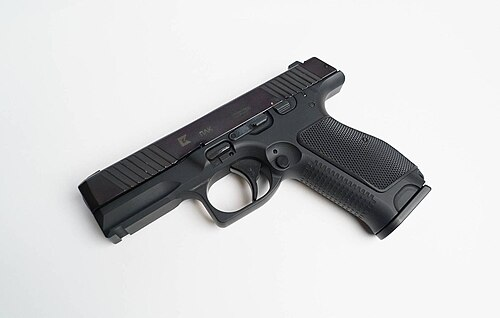
\includegraphics{../images/pistolety_i_pm/pl-15_1.jpg}
\caption{PL-15 Lebiediew --- pistolet 9×19 mm}
\end{figure}

\subsection{Opis}\label{opis-113}

PL-14 (Пистолет Лебедева --- Pistolet Lebiedewa), znany też jako PL-15 w
wersji wojskowej, to rosyjski pistolet samopowtarzalny kalibru 9×19 mm
Parabellum opracowany przez Dmitrija Lebiedewa w Konsorcjum Kałasznikowa
(Izhmash) i zaprezentowany w 2014 roku. Jest przeznaczony do programu
``Ratnik-3'' jako potencjalny zastępnik MP-443 Grach. Wyróżnia się
wyjątkowo płaskim profilem (21 mm grubości), ergonomicznym chwytem,
stałymi celownikami noktowizyjnymi i szyną Picatinny. PL-15K to skrócona
wersja dla oficerów i służb specjalnych. W 2020 roku FSB zamówiło partię
PL-15 --- rozpoczynając stopniowe wdrożenie jako zamiennik MP-443 w
jednostkach specjalnych.

\subsection{Dane techniczne}\label{dane-techniczne-113}

\begin{longtable}[]{@{}ll@{}}
\toprule\noalign{}
Parametr & Wartość \\
\midrule\noalign{}
\endhead
\bottomrule\noalign{}
\endlastfoot
Typ & Pistolet samopowtarzalny \\
Kraj produkcji & Rosja \\
Rok wprowadzenia & 2020 (ograniczone dostawy FSB) \\
Kaliber & 9×19 mm Parabellum \\
Długość & 206 mm \\
Szerokość & 21 mm \\
Długość lufy & 127 mm \\
Masa (bez magazynka) & 800 g \\
Pojemność magazynka & 15 lub 17 nabojów \\
Prędkość wylotowa & 460 m/s \\
Skuteczny zasięg & 50 m \\
\end{longtable}

\subsection{Charakterystyczne cechy
rozpoznawcze}\label{charakterystyczne-cechy-rozpoznawcze-113}

\begin{quote}
Jak odróżnić PL-14/15 od MP-443 i GSz-18:
\end{quote}

\begin{itemize}
\tightlist
\item
  \textbf{Wyjątkowo płaski profil 21 mm --- ``nowoczesny zachodnim
  stylem'':} PL-14/15 jest jednym z najcieńszych rosyjskich pistoletów;
  21 mm grubości jest porównywalny z zachodnimi pistoletami klasy
  premium (Walther PPQ, HK VP9); wyraźnie cieńszy od MP-443
  (\textasciitilde33 mm)
\item
  \textbf{Brak zewnętrznego kurka --- striker-fired hammerless:}
  PL-14/15 nie ma kurka zewnętrznego; tylna część slajdu jest gładka jak
  w GSz-18; to odróżnia od PM i MP-443 (z kurkami); ``gładki tył zamka''
  to identyfikator striker-fired
\item
  \textbf{Niska linia zamka (low bore axis) --- wyraźne cechy
  ergonomiczne:} PL-14/15 ma bardzo niską linię lufy nad chwytem ---
  chwyt sięga wyżej względem lufy; przy trzymaniu w dłoni kąt jest
  bardziej naturalny niż w MP-443; ta cecha jest widoczna przy
  porównaniu profili
\item
  \textbf{Szyna Picatinny pod lufą i stałe celowniki noktowizyjne:}
  PL-14/15 ma nowoczesną szynę i stałe trójpunktowe celowniki z tritową
  insercją; nowoczesny wygląd celownika (biały lub jasnożółty punkt)
  jest widoczny
\item
  \textbf{Bardzo nowy --- rzadko spotykany poza FSB i pokazami:} PL-15
  jest na etapie wdrożenia; poza FSB nie jest jeszcze masowo stosowany;
  widok tej broni sugeruje jednostkę specjalną najwyższej klasy lub
  wystawę branżową
\item
  \textbf{Estetyka ``premium'' --- bliżej Walther/HK niż PM:} PL-14/15
  estetycznie przypomina zachodnioeuropejski pistolet premium bardziej
  niż tradycyjny rosyjski projekt; ta ``zachodnia'' estetyka jest
  zaskakująca dla osoby znającej rosyjskie pistolety
\end{itemize}

\subsection{Ciekawostka}\label{ciekawostka-113}

\begin{quote}
PL-14 był kontrowersyjny od początku --- bo jego projektant Lebiedew
pracował dla Konsorcjum Kałasznikowa, tradycyjnie producenta karabinów,
nie pistoletów. KBP w Tule (tradycyjny producent rosyjskich pistoletów)
poczuło się urażone. W rosyjskich mediach branżowych toczył się przez
kilka lat spór: ``kto ma prawo robić pistolety dla armii?'' --- KBP
(tradycja i doświadczenie) czy Kałasznikow (marka i budżet)? W 2020 roku
wygrał Kałasznikow --- FSB zamówiło PL-15; ale KBP nadal dostarcza
MP-443 dla wojska. Rosja ma więc dwa ``nowe'' pistolety służbowe
równolegle.
\end{quote}

\section{Pistolet podwodny SPP-1M}\label{pistolet-podwodny-spp-1m}

\subsubsection{SPP-1M Underwater Pistol \textbar{}
СПП-1М}\label{spp-1m-underwater-pistol-ux441ux43fux43f-1ux43c}

\begin{center}\rule{0.5\linewidth}{0.5pt}\end{center}

\begin{figure}
\centering
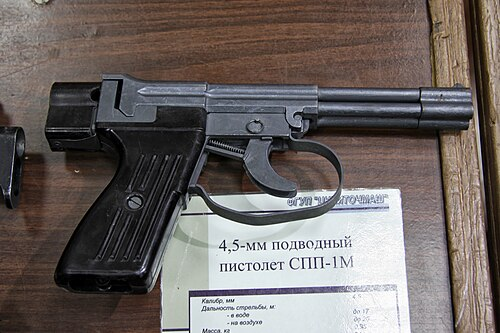
\includegraphics{../images/pistolety_i_pm/spp-1m_1.jpg}
\caption{SPP-1M --- pistolet podwodny}
\end{figure}

\subsection{Opis}\label{opis-114}

SPP-1M (Специальный Пистолет Подводный --- Specjalny Pistolet Podwodny)
to radziecki pistolet do strzelania pod wodą kalibru 4,5 mm SPS
opracowany przez TSNIITOCHMASH i przyjęty do służby w 1971 roku dla
płetwonurków bojowych i sił specjalnych marynarki wojennej. Używa
specjalnych igłowych pocisków SPS --- długich (120 mm), cienkich (4,5
mm) stalowych igieł stabilizowanych hydrodynamicznie w wodzie. Pod wodą
zasięg skuteczny wynosi 17 m na głębokości 5 m i spada do 6 m na
głębokości 40 m; na powierzchni zasięg to 20 m. SPP-1M ma cztery lufy
naraz (czterolufowy rewolwer) --- po jednej kulce w każdej lufie;
przeładowanie zajmuje kilka sekund i wymaga wymiany ``kasety''
czterolufowej. Stosowany przez rosyjskie wojska podwodne Spetsnaz.

\subsection{Dane techniczne}\label{dane-techniczne-114}

\begin{longtable}[]{@{}ll@{}}
\toprule\noalign{}
Parametr & Wartość \\
\midrule\noalign{}
\endhead
\bottomrule\noalign{}
\endlastfoot
Typ & Pistolet podwodny czterolufowy \\
Kraj produkcji & ZSRR / Rosja \\
Rok wprowadzenia & 1971 \\
Kaliber & 4,5 mm SPS (igłowy) \\
Długość & 244 mm \\
Masa (bez pocisków) & 950 g \\
Liczba luf & 4 \\
Pojemność & 4 naboje (po jednym w lufie) \\
Zasięg (5 m głębokości) & 17 m \\
Zasięg (40 m głębokości) & 6 m \\
Zasięg (nad wodą) & 20 m \\
\end{longtable}

\subsection{Charakterystyczne cechy
rozpoznawcze}\label{charakterystyczne-cechy-rozpoznawcze-114}

\begin{quote}
Jak odróżnić SPP-1M od standardowych pistoletów:
\end{quote}

\begin{itemize}
\tightlist
\item
  \textbf{Cztery widoczne otwory luf --- ``zestaw rur'' z przodu:}
  SPP-1M ma charakterystyczny blok czterech luf widoczny z przodu; żaden
  standardowy pistolet nie ma czterech luf; ten ``wiązkowy'' przód jest
  natychmiastowym identyfikatorem
\item
  \textbf{Igłowe pociski SPS --- wyjątkowo długie i cienkie:} pociski
  SPS mają 120 mm długości i 4,5 mm średnicy --- wyglądają jak metalowe
  igły lub cienkie gwoździe; przy załadowaniu lub obserwacji amunicji
  wyraźnie inne od standardowych nabojów pistoletowych
\item
  \textbf{Brak typowego zamka samopowtarzalnego --- rewolwerowa logika:}
  SPP-1M nie ma suwadła (slide) jak standardowy pistolet
  samopowtarzalny; kształt broni jest ``stały'' --- jak rewolwer z
  osłoną; brak ruchu zamka po strzale
\item
  \textbf{Prostokątny, ``pudełkowy'' kształt komory zamkowej z blokiem
  luf:} SPP-1M ma prosty prostokątny kształt bez wyraźnego
  ``pistolowego'' profilu; wyraźnie inna sylwetka od PM czy MP-443 ---
  mniej ``pistoletowy'' a bardziej ``narzędziowy'' wygląd
\item
  \textbf{Broń służby podwodnej --- widoczna wyłącznie u płetwonurków:}
  SPP-1M pojawia się tylko na fotografiach wojsk podwodnych lub
  prezentacjach specjalistycznego uzbrojenia; widok SPP-1M na żołnierzu
  od razu sugeruje płetwonurka bojowego
\item
  \textbf{Ciemnoszare lub czarne metalowe wykończenie bez plastiku:}
  SPP-1M jest w całości metalowy (aluminium i stal); brak plastikowych
  elementów różni go od nowoczesnych pistoletów polimerowych
\end{itemize}

\subsection{Ciekawostka}\label{ciekawostka-114}

\begin{quote}
SPP-1M jest bronią tak niszową, że przez dekady zachodnie wywiady nie
były pewne jej istnienia --- sowieccy płetwonurkowie Spetsnaz używali
jej w najgłębszej tajemnicy. Pierwsza potwierdzona fotografia SPP-1M
pojawiła się na zachodzie dopiero na początku lat 90. po rozpadzie ZSRR.
Dla zachodnich specjalistów od uzbrojenia był to szok --- okazało się,
że ZSRR miał kompletny arsenał broni podwodnej (SPP-1M na pistolet, APS
na karabin szturmowy, podwodne noże bojowe), o którym Zachód nie
wiedział nic przez 20 lat.
\end{quote}

\section{Podwodny karabinek APS}\label{podwodny-karabinek-aps}

\subsubsection{APS Underwater Assault Rifle \textbar{} АПС (Автомат
Подводный
Специальный)}\label{aps-underwater-assault-rifle-ux430ux43fux441-ux430ux432ux442ux43eux43cux430ux442-ux43fux43eux434ux432ux43eux434ux43dux44bux439-ux441ux43fux435ux446ux438ux430ux43bux44cux43dux44bux439}

\begin{center}\rule{0.5\linewidth}{0.5pt}\end{center}

\begin{figure}
\centering
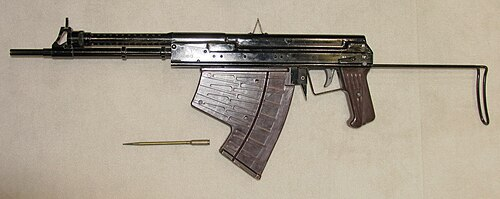
\includegraphics{../images/pistolety_i_pm/sps-underwater_1.jpg}
\caption{APS podwodny --- karabinek podwodny}
\end{figure}

\subsection{Opis}\label{opis-115}

APS (Автомат Подводный Специальный --- Automatyczny Karabinek Podwodny
Specjalny, nie mylić z pistoletem APS Steczkin) to radziecki karabin
szturmowy do strzelania pod wodą kalibru 5,66 mm MPS opracowany przez
TsNIITochMash i przyjęty do służby w 1975 roku dla płetwonurków
bojowych. Używa specjalnych igłowych pocisków MPS (120 mm długości)
stabilizowanych hydrodynamicznie w wodzie --- identyczna zasada jak
SPP-1M, ale w wersji automatycznej. Pod wodą na głębokości 5 m zasięg to
30 m; na 40 m --- 11 m. Na powietrzu broń działa, ale celność i zasięg
są mocno ograniczone (igły nie są stabilizowane przez lotki na
powietrzu). Od ok. 2000 roku trwa zastępowanie przez ASM-DT ``Morski
Lew'' który jest skuteczny zarówno pod wodą jak i na lądzie.

\subsection{Dane techniczne}\label{dane-techniczne-115}

\begin{longtable}[]{@{}ll@{}}
\toprule\noalign{}
Parametr & Wartość \\
\midrule\noalign{}
\endhead
\bottomrule\noalign{}
\endlastfoot
Typ & Automatyczny karabin podwodny \\
Kraj produkcji & ZSRR / Rosja \\
Rok wprowadzenia & 1975 \\
Kaliber & 5,66 mm MPS (igłowy) \\
Długość & 823 mm \\
Długość lufy & 300 mm \\
Masa (bez magazynka) & 2,46 kg \\
Pojemność magazynka & 26 nabojów \\
Szybkostrzelność & 600 strz./min \\
Zasięg (5 m głęb.) & 30 m \\
Zasięg (40 m głęb.) & 11 m \\
\end{longtable}

\subsection{Charakterystyczne cechy
rozpoznawcze}\label{charakterystyczne-cechy-rozpoznawcze-115}

\begin{quote}
Jak odróżnić APS podwodny od AKS-74U i broni specjalnej:
\end{quote}

\begin{itemize}
\tightlist
\item
  \textbf{Wyraźnie inne proporcje --- ``zbyt długi i wąski'' karabin:}
  APS podwodny ma bardzo długi, wąski wygląd z wyraźnie krótszą komorą
  niż długi magazynek; proporcje są inne od wszystkich karabinów AK
\item
  \textbf{Igłowe pociski 5,66 mm widoczne w magazynku:} magazynek APS
  podwodnego wygląda inaczej --- jest wąski i długi proporcjonalnie do
  pocisków-igieł; naboje MPS są długie i cienkie; widoczne przez okienko
  magazynka lub przy załadowaniu
\item
  \textbf{Brak gazownika i innych typowych elementów AK:} APS podwodny
  nie ma klasycznego gazownika AK nad lufą; układ gazowy jest ukryty lub
  inaczej rozwiązany; brak charakterystycznej ``opuszki'' gazownika AK
\item
  \textbf{Prosta, ``rurowa'' konstrukcja bez bocznych szyn i elementów:}
  APS podwodny jest prostym ``narzędziem bojowym'' bez szyn, bez
  ergonomicznych uchwytów --- bo pod wodą ergonomia jest inna; prosta,
  ``utylitarna'' budowa
\item
  \textbf{Broń widoczna wyłącznie u płetwonurków bojowych:} APS podwodny
  pojawia się wyłącznie w kontekście jednostek podwodnych Spetsnaz;
  widok tej broni na żołnierzu od razu identyfikuje płetwonurka bojowego
  lub prezentację specjalistycznego uzbrojenia
\item
  \textbf{Prosta, nieregulowana plastikowa kolba:} kolba APS jest prosta
  i nieregulowana --- inna od składanych i regulowanych kolb AKS i
  AK-12; brak mechanizmów składania (pod wodą kolba jest zawsze
  rozłożona)
\end{itemize}

\subsection{Ciekawostka}\label{ciekawostka-115}

\begin{quote}
APS podwodny był jednym z najbardziej skrywanych sekretów ZSRR przez
lata 70.--80. --- bo jego istnienie ujawniałoby plany sowieckich
operacji podwodnych: sabotaż portów, niszczenie infrastruktury
podwodnej, likwidacja nurków wroga. Kiedy APS pojawił się po raz
pierwszy publicznie w latach 90., zachodni eksperci byli zdumieni: nikt
nie wiedział, że Sowieci mają kompletny system broni podwodnej
automatycznej. NATO natychmiast zaczęło planować odpowiedź --- ale do
dziś zachodni odpowiednik APS jest mniej zaawansowany; USA mają HK P11
(pistolet), ale nie mają automatycznej podwodnej broni porównywalnej z
APS.
\end{quote}

\section{Granat ręczny F-1}\label{granat-rux119czny-f-1}

\subsubsection{F-1 Hand Grenade \textbar{} Ф-1
(«Лимонка»)}\label{f-1-hand-grenade-ux444-1-ux43bux438ux43cux43eux43dux43aux430}

\begin{center}\rule{0.5\linewidth}{0.5pt}\end{center}

\begin{figure}
\centering
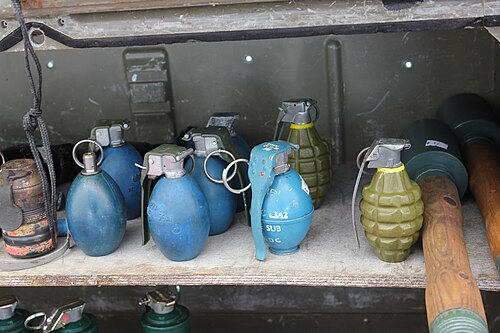
\includegraphics{../images/granaty_reczne/f-1_1.jpg}
\caption{F-1 Limonka --- granat defensywny}
\end{figure}

\subsection{Opis}\label{opis-116}

F-1 (Ф-1, potocznie ``Limonka'' --- Cytrynka) to radziecki defensywny
odłamkowy granat ręczny z żeliwną obudową rowkowaną, opracowany w ZSRR w
latach 40. na bazie francuskiego granatu F1 (stąd oznaczenie) i przyjęty
masowo do służby. Jest to granat defensywny --- zasięg odłamków do 200
m, wymagający ukrycia strzelca za przeszkodą po rzucie. Rowkowana
żeliwna obudowa rozpada się na ok. 290 ciężkich odłamków zdolnych do
rażenia na duże odległości. F-1 używa standardowego zapalnika UZRGM
(3,2--4,2 s opóźnienia). Jest jednym z najbardziej rozpoznawalnych
granatów ręcznych na świecie --- stosowany w ponad 50 krajach i przez
niezliczone siły nieregularne; produkowany masowo przez ZSRR przez
dekady.

\subsection{Dane techniczne}\label{dane-techniczne-116}

\begin{longtable}[]{@{}ll@{}}
\toprule\noalign{}
Parametr & Wartość \\
\midrule\noalign{}
\endhead
\bottomrule\noalign{}
\endlastfoot
Typ & Odłamkowy granat ręczny (defensywny) \\
Kraj produkcji & ZSRR / Rosja \\
Rok wprowadzenia & lata 40. \\
Masa & 600 g \\
Masa ładunku & 60 g TNT \\
Długość & 130 mm \\
Średnica & 55 mm \\
Czas opóźnienia zapalnika & 3,2--4,2 s \\
Zasięg odłamków & do 200 m \\
Zasięg rzutu & 20--40 m \\
\end{longtable}

\subsection{Charakterystyczne cechy
rozpoznawcze}\label{charakterystyczne-cechy-rozpoznawcze-116}

\begin{quote}
Jak odróżnić F-1 od RGD-5 i zachodnich granatów:
\end{quote}

\begin{itemize}
\tightlist
\item
  \textbf{Charakterystyczna ``ananasowa'' siatka rowków na obudowie:}
  F-1 ma ikoniczną rowkowaną żeliwną obudowę --- pionowe i poziome rowki
  tworzące charakterystyczną kratkę ``ananasową''; RGD-5 jest gładki; ta
  rowkowana faktura jest absolutnym identyfikatorem F-1
\item
  \textbf{Cięższy od RGD-5 --- 600 g vs 310 g:} F-1 jest prawie dwa razy
  cięższy od RGD-5; przy trzymaniu w dłoni różnica masy jest natychmiast
  wyczuwalna; ciężar F-1 jest charakterystyczny
\item
  \textbf{Cytrynowaty kształt --- nie jajko, ale ``cytryna'':} F-1 ma
  charakterystyczny kształt przypominający cytrynę --- lekko podłużny,
  nieco spłaszczony; stąd potoczna nazwa ``Limonka''; RGD-5 jest
  bardziej ``jajowaty''
\item
  \textbf{Żeliwna obudowa --- ciemnostalowa lub szara barwa:} F-1 ma
  charakterystyczną ciemnostalową lub szarawą barwę żeliwa --- inną od
  ciemnozielonej stali RGD-5; przy porównaniu tekstura powierzchni jest
  też inna (żeliwo vs stal)
\item
  \textbf{Ten sam zapalnik UZRGM co RGD-5 --- góra granatu wygląda
  identycznie:} zapalnik na górze F-1 i RGD-5 jest identyczny (UZRGM);
  patrząc tylko na zapalnik nie można odróżnić; różnica jest w korpusie
  granatu
\item
  \textbf{Defensywny --- rzucany z ukrycia, nie z otwartego terenu:} F-1
  ze względu na zasięg odłamków 200 m jest używany wyłącznie z ukrycia
  za solidną przeszkodą; żołnierz rzucający F-1 na otwartym terenie
  naraża siebie; ta taktyczna właściwość odróżnia F-1 od ``ofensywnego''
  RGD-5
\end{itemize}

\subsection{Ciekawostka}\label{ciekawostka-116}

\begin{quote}
F-1 ``Limonka'' stała się symbolem rosyjskiej przestępczości
zorganizowanej lat 90. --- bo była masowo dostępna na czarnym rynku po
rozpadzie ZSRR. Magazyny wojskowe były rozkradane tysiącami; F-1
kosztowała na czarnym rynku kilka dolarów. W efekcie ``Limonki'' były
używane do zastraszania i eliminowania rywali przez grupy gangsterskie w
całej byłej FSB. Rosyjska policja szacowała, że w samej Moskwie
skradziono w latach 1992--1996 ponad 100 000 granatów F-1 z magazynów
wojskowych --- z czego część nigdy nie odzyskano.
\end{quote}

\section{Granat ręczny RGD-5}\label{granat-rux119czny-rgd-5}

\subsubsection{RGD-5 Hand Grenade \textbar{}
РГД-5}\label{rgd-5-hand-grenade-ux440ux433ux434-5}

\begin{center}\rule{0.5\linewidth}{0.5pt}\end{center}

\begin{figure}
\centering
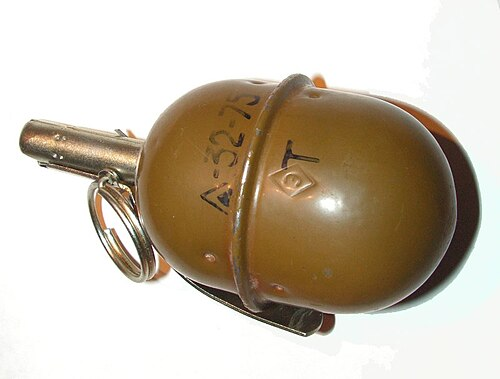
\includegraphics{../images/granaty_reczne/rgd-5_1.jpg}
\caption{RGD-5 --- granat ofensywny}
\end{figure}

\subsection{Opis}\label{opis-117}

RGD-5 (Ручная Граnatа Дистанционная-5) to radziecki odłamkowy granat
ręczny z zapalnikiem czasowym UZRGM, opracowany w końcu lat 40. i
przyjęty do służby w 1954 roku jako zastępnik granatu RG-42. Jest
standardowym ofensywnym granatem ręcznym radzieckiej i rosyjskiej armii
przez ponad 70 lat. Stalowa koperta rozrywa się na odłamki --- zasięg
rozrzutu odłamków 15--20 m (granat ofensywny, rażenie mniejsze niż F-1).
Zapalnik UZRGM daje 3,2--4,2 sekundy opóźnienia od wyciągnięcia
zawleczki do wybuchu. RGD-5 jest masowo eksportowany --- stosowany przez
armie ponad 40 państw i setki nieregularnych sił zbrojnych na całym
świecie.

\subsection{Dane techniczne}\label{dane-techniczne-117}

\begin{longtable}[]{@{}ll@{}}
\toprule\noalign{}
Parametr & Wartość \\
\midrule\noalign{}
\endhead
\bottomrule\noalign{}
\endlastfoot
Typ & Odłamkowy granat ręczny (ofensywny) \\
Kraj produkcji & ZSRR / Rosja \\
Rok wprowadzenia & 1954 \\
Masa & 310 g \\
Masa ładunku & 110 g TNT \\
Długość & 117 mm \\
Średnica & 58 mm \\
Czas opóźnienia zapalnika & 3,2--4,2 s \\
Zasięg odłamków & 15--20 m \\
Zasięg rzutu & 30--50 m \\
\end{longtable}

\subsection{Charakterystyczne cechy
rozpoznawcze}\label{charakterystyczne-cechy-rozpoznawcze-117}

\begin{quote}
Jak odróżnić RGD-5 od F-1 i zachodnich granatów:
\end{quote}

\begin{itemize}
\tightlist
\item
  \textbf{Gładka jajowata / cylindryczna obudowa bez rowkowania:} RGD-5
  ma gładką stalową obudowę bez charakterystycznej ``ananasowej'' siatki
  rowków jak F-1; kształt jest jajowaty lub cylindryczno-stożkowy; ta
  gładkość jest kluczowym wyróżnikiem od F-1
\item
  \textbf{Mniejszy i lżejszy od F-1 --- 310 g vs 600 g:} RGD-5 jest
  wyraźnie mniejszy i lżejszy od F-1; przy trzymaniu obu granatów naraz
  różnica masy (niemal 2:1) jest natychmiast wyczuwalna
\item
  \textbf{Zapalnik UZRGM z metalową kapsułką i zawleczką --- standardowy
  radziecki:} zapalnik UZRGM jest standardowy dla rodziny radzieckich
  granatów; charakterystyczny metalowy ``kapturek'' zapalnika na górze
  granatu z zawleczką po boku
\item
  \textbf{Zielono-oliwkowy kolor z czarnym lub żółtym oznaczeniem:}
  RGD-5 ma zazwyczaj ciemnooliwkowy (khaki) kolor; na górze lub boku
  widoczne oznaczenia (czasem żółte paski wskazujące typ ładunku); F-1
  ma podobny kolor, ale inną fakturę powierzchni
\item
  \textbf{Jajowaty kształt --- ``jajko granatowe'':} sylwetka RGD-5 jest
  typowym ``jajkiem'' --- zaokrąglony dół, nieco zwężający się ku górze
  zapalnika; F-1 jest bardziej cylindryczny z wyraźnym ulistnieniem
  rowków
\item
  \textbf{Zasięg rozrzutu 15--20 m --- granat ``ofensywny'':} RGD-5 ma
  mniejszy zasięg odłamków niż F-1 (do 200 m); dlatego można go rzucić z
  otwartego terenu bez ukrycia; F-1 wymaga ukrycia po rzucie ze względu
  na duży zasięg odłamków
\end{itemize}

\subsection{Ciekawostka}\label{ciekawostka-117}

\begin{quote}
RGD-5 ma jedną słabość, która kosztowała życie wielu żołnierzy
radzieckich w Afganistanie --- krótka zawleczka łatwo wypadała przy
noszeniu w kieszeni lub plecaku bez specjalnej kabury. Wypadnięcie
zawleczki bez zapalnika UZRGM nie powoduje wybuchu --- ale wypadnięcie
zawleczki Z zapalnikiem już tak. W rezultacie w Afganistanie wprowadzono
obowiązek noszenia granatów w specjalnych kasetach i zabezpieczania
zawleczki taśmą. Ta prosta poprawka --- kawałek taśmy na zawleczce ---
uratowała więcej żołnierzy radzieckich niż niejeden nowy system broni.
\end{quote}

\section{Granat ręczny RGN}\label{granat-rux119czny-rgn}

\subsubsection{RGN Hand Grenade \textbar{} РГН (Ручная Граната
Наступательная)}\label{rgn-hand-grenade-ux440ux433ux43d-ux440ux443ux447ux43dux430ux44f-ux433ux440ux430ux43dux430ux442ux430-ux43dux430ux441ux442ux443ux43fux430ux442ux435ux43bux44cux43dux430ux44f}

\begin{center}\rule{0.5\linewidth}{0.5pt}\end{center}

\begin{figure}
\centering
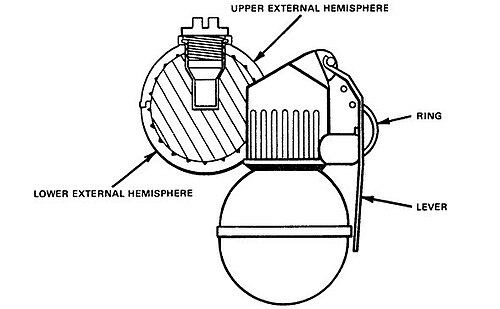
\includegraphics{../images/granaty_reczne/rgn_1.jpg}
\caption{RGN --- granat ofensywny z zapalnikiem uderzeniowym}
\end{figure}

\subsection{Opis}\label{opis-118}

RGN (Ручная Граната Наступательная --- Ręczny Granat Natarcia) to
radziecki ofensywny granat ręczny z zapalnikiem udarowo-czasowym
opracowany w TsNIITochMash i przyjęty do służby w 1981 roku jako
modernizacja RGD-5. Wyróżnia się zapalnikiem uderzeniowym UD (ударный
детонатор) --- granat wybucha przy uderzeniu w cel (przy padaniu na
ziemię lub w przeszkodę), bez czekania na wygaśnięcie zapalnika
czasowego; jeśli udar nie zadziała, jako rezerwa aktywuje się zapalnik
czasowy (3,5 s). Dwuczłonowa aluminiowa obudowa z wewnętrzną warstwą
odłamkującą daje jednolitą chmurę odłamków. Zasięg rażenia podobny do
RGD-5 (15--20 m), ale zapalnik uderzeniowy eliminuje problem ``toczącego
się granatu z opóźnieniem''.

\subsection{Dane techniczne}\label{dane-techniczne-118}

\begin{longtable}[]{@{}ll@{}}
\toprule\noalign{}
Parametr & Wartość \\
\midrule\noalign{}
\endhead
\bottomrule\noalign{}
\endlastfoot
Typ & Ofensywny granat ręczny z zapalnikiem uderzeniowym \\
Kraj produkcji & ZSRR / Rosja \\
Rok wprowadzenia & 1981 \\
Masa & 310 g \\
Masa ładunku & 114 g A-IX-1 \\
Długość & 113 mm \\
Średnica & 60 mm \\
Zapalnik & Uderzeniowy + czasowy 3,5 s rezerwa \\
Zasięg odłamków & 15--20 m \\
Zasięg rzutu & 25--45 m \\
\end{longtable}

\subsection{Charakterystyczne cechy
rozpoznawcze}\label{charakterystyczne-cechy-rozpoznawcze-118}

\begin{quote}
Jak odróżnić RGN od RGD-5 i RGO:
\end{quote}

\begin{itemize}
\tightlist
\item
  \textbf{Aluminiowa obudowa w dwóch kształtach ze szwem pośrodku:} RGN
  ma charakterystyczną dwuczłonową aluminiową obudowę --- dolna półkula
  połączona z górną z wyraźnym ``szwem'' pośrodku; RGD-5 ma
  jednoczęściową stalową obudowę; ten szew jest identyfikatorem całej
  rodziny RGN/RGO
\item
  \textbf{Brak rowkowania --- gładka z zaznaczonym szwem:} RGN jest
  gładki jak RGD-5 (bez rowkowania jak F-1), ale z charakterystycznym
  szwem środkowym; wizualnie ``gładka kula z linią pośrodku''
\item
  \textbf{Aluminiowy matowy kolor --- srebrzysto-szary zamiast stalowego
  zielonego:} RGN jest z aluminium; kolor jest srebrzysto-szary lub
  ciemnoszary z matowym wykończeniem; RGD-5 jest ciemnozielony; F-1 ---
  stalowoszary żeliwo; kolor aluminium jest charakterystyczny
\item
  \textbf{Zapalnik z ``nitką'' do uzbrojeniana --- widoczna zmiana w
  zapalnikowym kapturku:} zapalnik RGN ma nieco inny wygląd niż UZRGM
  granatu RGD-5; kapturek zapalnika ma inną geometrię; subtelna różnica
  w kształcie zapalnika
\item
  \textbf{Mniejszy zasięg odłamków niż F-1 --- ofensywny charakter:} jak
  RGD-5, RGN jest ofensywny i można go rzucić z otwartego terenu; F-1
  wymaga ukrycia; ta właściwość taktyczna nie jest wizualna, ale jest
  ważną informacją operacyjną
\item
  \textbf{Rzadziej widoczny niż F-1 i RGD-5 --- nowszy i mniej
  powszechny:} RGN jest relatywnie nowszy i produkowany w mniejszych
  ilościach; na polach walki częściej widać F-1 i RGD-5 ze starszych
  zapasów
\end{itemize}

\subsection{Ciekawostka}\label{ciekawostka-118}

\begin{quote}
RGN (i RGO) zostały opracowane po doświadczeniach z Afganistanu, gdzie
żołnierze radzieccy narzekali na jeden problem z RGD-5 i F-1: po rzucie
granat toczył się po nierównym terenie skalnym lub piasku, oddalając się
od celu przed eksplozją --- co zmniejszało skuteczność. Granat z
zapalnikiem uderzeniowym wybucha przy pierwszym kontakcie z ziemią lub
przeszkodą --- bez toczenia i bez opóźnienia. Ta prosta zmiana znacząco
poprawiła skuteczność w górzystym afgańskim terenie, gdzie toczące się
granaty były prawdziwym problemem.
\end{quote}

\section{Granat ręczny RGO}\label{granat-rux119czny-rgo}

\subsubsection{RGO Hand Grenade \textbar{} РГО (Ручная Граната
Оборонительная)}\label{rgo-hand-grenade-ux440ux433ux43e-ux440ux443ux447ux43dux430ux44f-ux433ux440ux430ux43dux430ux442ux430-ux43eux431ux43eux440ux43eux43dux438ux442ux435ux43bux44cux43dux430ux44f}

\begin{center}\rule{0.5\linewidth}{0.5pt}\end{center}

\begin{figure}
\centering
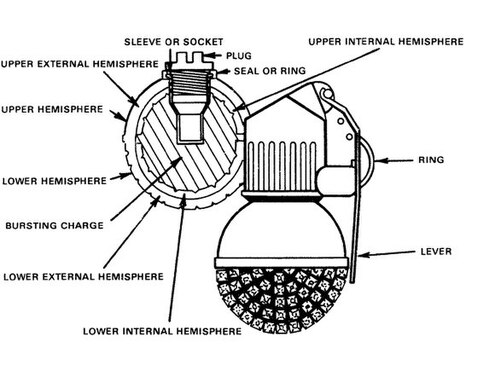
\includegraphics{../images/granaty_reczne/rgo_1.jpg}
\caption{RGO --- granat defensywny z zapalnikiem uderzeniowym}
\end{figure}

\subsection{Opis}\label{opis-119}

RGO (Ручная Граната Оборонительная --- Ręczny Granat Obrony) to
radziecki defensywny granat ręczny z zapalnikiem udarowo-czasowym
opracowany w TsNIITochMash i przyjęty do służby w 1981 roku jako para
dla RGN. RGO jest defensywną wersją --- cięższy (530 g) i z większym
zasięgiem odłamków (do 150 m) dzięki wewnętrznej żeliwnej wkładce
fragmentacyjnej. Jak RGN, ma zapalnik uderzeniowy + zapalnik czasowy 3,5
s jako rezerwa. Czterosegmentowa wkładka żeliwna i aluminiowa obudowa
zewnętrzna dają łącznie gęstszą chmurę odłamków niż F-1 przy podobnej
masie. RGO jest bardziej śmiercionośny od RGN w terenie otwartym ---
wymagający ukrycia po rzucie.

\subsection{Dane techniczne}\label{dane-techniczne-119}

\begin{longtable}[]{@{}ll@{}}
\toprule\noalign{}
Parametr & Wartość \\
\midrule\noalign{}
\endhead
\bottomrule\noalign{}
\endlastfoot
Typ & Defensywny granat ręczny z zapalnikiem uderzeniowym \\
Kraj produkcji & ZSRR / Rosja \\
Rok wprowadzenia & 1981 \\
Masa & 530 g \\
Masa ładunku & 92 g A-IX-1 \\
Długość & 130 mm \\
Średnica & 61 mm \\
Zapalnik & Uderzeniowy + czasowy 3,5 s rezerwa \\
Zasięg odłamków & do 150 m \\
Zasięg rzutu & 20--40 m \\
\end{longtable}

\subsection{Charakterystyczne cechy
rozpoznawcze}\label{charakterystyczne-cechy-rozpoznawcze-119}

\begin{quote}
Jak odróżnić RGO od RGN i F-1:
\end{quote}

\begin{itemize}
\tightlist
\item
  \textbf{Dwuczłonowa obudowa jak RGN --- ale cięższy (530 g vs 310 g):}
  RGO i RGN mają identyczną aluminiową dwuczłonową obudowę z
  charakterystycznym szwem środkowym; różnica jest w masie --- RGO jest
  wyraźnie cięższy; przy trzymaniu obu naraz różnica 220 g jest
  wyczuwalna
\item
  \textbf{Identyczny szew środkowy jak RGN --- klucz do odróżnienia od
  F-1 i RGD-5:} szew środkowy jest wspólny dla RGN i RGO; F-1 i RGD-5
  nie mają szwu; jeśli granat ma szew --- to RGN lub RGO
\item
  \textbf{Aluminiowa obudowa z szarawym lub ciemnooliwkowym
  wykończeniem:} RGO jak RGN jest z aluminium; kolor jest
  szarawooliwkowy lub matowoszary; wizualnie podobny do RGN, ale
  zidentyfikowany przez masę i oznaczenia
\item
  \textbf{Oznaczenia na granatie wskazują typ (N --- natarcie, O ---
  obrona):} na górnej części obudowy lub zapalnika rosyjskie granaty
  mają oznaczenia; ``N'' lub ``RGN'' to ofensywny, ``O'' lub ``RGO'' to
  defensywny; przy bliskim oglądaniu lub znajomości oznaczeń to kluczowy
  wyróżnik
\item
  \textbf{Zasięg odłamków 150 m --- nie rzucać bez ukrycia:} RGO wymaga
  ukrycia za solidną przeszkodą po rzucie; ten wymóg taktyczny odróżnia
  RGO od ofensywnego RGN; żołnierz rzucający RGO na otwartym terenie
  jest zagrożony własną bronią
\item
  \textbf{Para dla RGN --- oba granaty często transportowane razem:}
  rosyjskie oddziały często noszą zestawy RGN + RGO; widok dwóch
  granatów ze szwem środkowym przy żołnierzu to prawdopodobnie właśnie
  ta para
\end{itemize}

\subsection{Ciekawostka}\label{ciekawostka-119}

\begin{quote}
RGO rozwiązał ``problem defensywny'' F-1 w Afganistanie --- analogicznie
do RGN dla ofensywnych. F-1 z zapalnikiem czasowym 4 sekundy dawał
mudżahedinom czas na ucieczkę przed eksplozją jeśli granat wylądował w
ich pobliżu. RGO z zapalnikiem uderzeniowym niszczy cel natychmiast po
kontakcie z ziemią --- bez sekundy na ucieczkę. Rosyjscy żołnierze w
Czeczenii chwalili RGO za właśnie to --- ``jak wyciągam zawleczkę i
rzucam, to on wybucha gdy trafia, nie sekundy później''. Ta właściwość
jest szczególnie cenna przy oczyszczaniu budynków, gdzie sekundy
opóźnienia mogą kosztować życie.
\end{quote}

\section{Granat przeciwpancerny
RKG-3}\label{granat-przeciwpancerny-rkg-3}

\subsubsection{RKG-3 Anti-Tank Hand Grenade \textbar{}
РКГ-3}\label{rkg-3-anti-tank-hand-grenade-ux440ux43aux433-3}

\begin{center}\rule{0.5\linewidth}{0.5pt}\end{center}

\begin{figure}
\centering
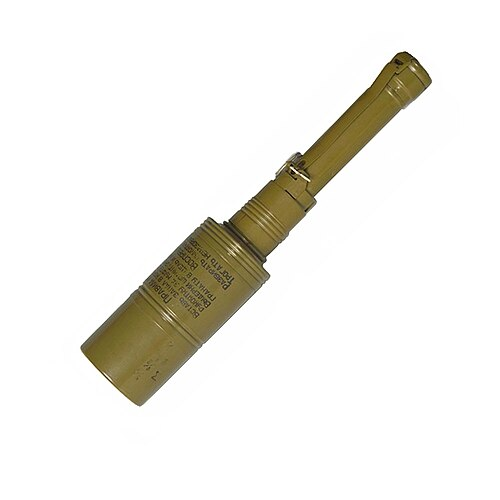
\includegraphics{../images/granaty_reczne/rkg-3_1.jpg}
\caption{RKG-3 --- granat przeciwpancerny kumulacyjny}
\end{figure}

\subsection{Opis}\label{opis-120}

RKG-3 (Ручная Кумулятивная Граната-3 --- Ręczny Granat Kumulacyjny-3) to
radziecki ręczny granat przeciwpancerny z głowicą kumulacyjną HEAT,
opracowany w 1950 roku. Wyróżnia się stabilizatorem paraszutowym --- po
rzucie rozkłada się mały paraszut (baldachim) zapewniający prawidłową
orientację głowicy kumulacyjnej prostopadle do pancerza przy uderzeniu;
bez prawidłowej orientacji głowica kumulacyjna jest nieefektywna. RKG-3
przebija do 75 mm pancerza jednolitego (wersja RKG-3M: 170 mm), co
wystarczało do rażenia czołgów II wojny światowej i wczesnych
powojennnych --- ale jest niewystarczające wobec nowoczesnych czołgów z
pancerzem reaktywnym. Nadal stosowany przez nieregularne siły zbrojne i
w konfliktach niskointensywnych.

\subsection{Dane techniczne}\label{dane-techniczne-120}

\begin{longtable}[]{@{}ll@{}}
\toprule\noalign{}
Parametr & Wartość \\
\midrule\noalign{}
\endhead
\bottomrule\noalign{}
\endlastfoot
Typ & Ręczny granat przeciwpancerny (HEAT) \\
Kraj produkcji & ZSRR \\
Rok wprowadzenia & 1950 \\
Masa & 771 g \\
Masa ładunku & 567 g RDX/TNT \\
Długość & 362 mm \\
Przenikanie pancerza & 75 mm (RKG-3) / 170 mm (RKG-3M) \\
Zasięg rzutu & 15--20 m \\
Zapalnik & Uderzeniowy, bez opóźnienia \\
\end{longtable}

\subsection{Charakterystyczne cechy
rozpoznawcze}\label{charakterystyczne-cechy-rozpoznawcze-120}

\begin{quote}
Jak odróżnić RKG-3 od granatów odłamkowych:
\end{quote}

\begin{itemize}
\tightlist
\item
  \textbf{Cylindryczny kształt z rączką --- wyraźnie inny od ``jajka''
  F-1 i RGD-5:} RKG-3 ma charakterystyczny cylindryczny kształt z długą
  rączką do rzutu; wygląda jak ``mała bomba'' lub ``puszka na kijku'';
  zupełnie inny od zaokrąglonych granatów F-1, RGD-5, RGN
\item
  \textbf{Stabilizator paraszutowy --- charakterystyczny ``baldachim''
  po rzucie:} po rzucie z RKG-3 rozkłada się mały kolorowy (zazwyczaj
  żółty lub pomarańczowy) paraszut stabilizujący orientację głowicy;
  widok ``lecącego granatu z paraszutem'' jest absolutnie unikalny i
  identyfikuje RKG-3
\item
  \textbf{Wyraźna długa rączka drewniana lub plastikowa:} RKG-3 ma
  charakterystyczną długą rączkę (ok. 15 cm) umożliwiającą rzut z siłą;
  żadny granat odłamkowy nie ma tak długiej rączki; wygląd jest zbliżony
  do (ale inny od) granatów trzonkowych WWII
\item
  \textbf{Charakterystyczny nosek kumulacyjny z przodu ---
  piezoelektryczny zapalnik:} front RKG-3 ma charakterystyczny stożkowy
  nosek z zapalnikiem uderzeniowym na szczycie; ta ``iglicowa'' forma
  przodu jest widoczna przy bliskim oglądaniu
\item
  \textbf{Wyraźnie cięższy od RGD-5 --- 771 g vs 310 g:} RKG-3 jest
  ponad dwa razy cięższy od RGD-5; rzucony zasięgiem tylko 15--20 m (vs
  30--50 m RGD-5) ze względu na masę; krótki zasięg rzutu jest istotną
  informacją taktyczną
\item
  \textbf{Broń coraz rzadsza --- widoczna głównie u nieregularnych sił
  zbrojnych:} RKG-3 jest przestarzała wobec nowoczesnych czołgów;
  pojawia się u nieregularnych sił zbrojnych i na rynku czarnym; widok
  tej broni sugeruje starszy arsenał lub siły nieregularne
\end{itemize}

\subsection{Ciekawostka}\label{ciekawostka-120}

\begin{quote}
RKG-3 zyskała nowe ``życie'' w Iraku w 2004--2008 roku, gdy bojownicy
iraccy opracowali taktykę rzucania ich z dachów budynków na
przejeżdżające americańskie Hummee i MRAP. Granaty stabilizowane
paraszutem trafiały w górne, słabiej opancerzone partie pojazdów. US
Army była zaskoczona --- bo RKG-3 był bronią z lat 50. uważaną za
przestarzałą. W odpowiedzi USA przyspieszyły montaż klatek ochronnych
(slat armor) na pojazdach, które zatrzymują granat przed dotarciem do
pancerza. Ta ``stara broń, nowa taktyka'' jest klasycznym przykładem
asymetrycznej adaptacji.
\end{quote}

\section{Granat do granatnika VOG-25}\label{granat-do-granatnika-vog-25}

\subsubsection{VOG-25 Grenade Round \textbar{}
ВОГ-25}\label{vog-25-grenade-round-ux432ux43eux433-25}

\begin{center}\rule{0.5\linewidth}{0.5pt}\end{center}

\begin{figure}
\centering
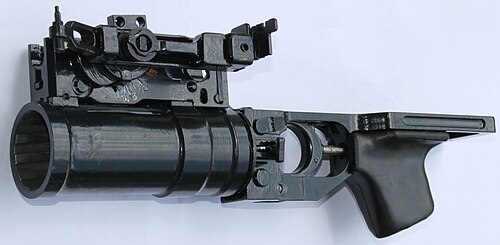
\includegraphics{../images/granaty_reczne/vog-25_1.jpg}
\caption{VOG-25 --- nabój do granatnika podlufowego}
\end{figure}

\subsection{Opis}\label{opis-121}

VOG-25 (Выстрел Осколочный Граnatомётный-25 --- Nabój Odłamkowy do
Granatnika-25) to radziecki nabój do granatników podlufowych GP-25,
GP-30 i GP-34 kalibru 40 mm, opracowany w KBP i przyjęty do użytku w
1978 roku razem z GP-25. Jest standardową amunicją odłamkową do
granatników nasadkowych rodziny GP --- wystrzelony ze łzawicy wylotowej
nabój leci balistycznie do 400 m i eksploduje przy uderzeniu, rażąc
odłamkami w promieniu 6 m. Wersja VOG-25P (Подпрыгивающий ---
Podskakujący) ma zapalnik udarowy z opóźnieniem --- granat odbija się od
ziemi i wybucha 0,5--1 m nad nią (airburst), rażąc skuteczniej okopy i
zasłoniętą piechotę. Stosowany masowo przez armię rosyjską i wszystkie
siły posiadające granatniki GP.

\subsection{Dane techniczne}\label{dane-techniczne-121}

\begin{longtable}[]{@{}ll@{}}
\toprule\noalign{}
Parametr & Wartość \\
\midrule\noalign{}
\endhead
\bottomrule\noalign{}
\endlastfoot
Typ & Nabój odłamkowy do granatnika podlufowego \\
Przeznaczenie & GP-25, GP-30, GP-34 (kaliber 40 mm) \\
Kraj produkcji & ZSRR / Rosja \\
Rok wprowadzenia & 1978 \\
Kaliber & 40×46 mm \\
Masa naboju & 250 g \\
Prędkość wylotowa & 76 m/s \\
Zasięg maks. & 400 m \\
Zasięg rażenia odłamkami & 6 m \\
Zapalnik & Uderzeniowy (VOG-25) / Uderzeniowy + airburst (VOG-25P) \\
\end{longtable}

\subsection{Charakterystyczne cechy
rozpoznawcze}\label{charakterystyczne-cechy-rozpoznawcze-121}

\begin{quote}
Jak odróżnić VOG-25 od granatów ręcznych i innych nabojów:
\end{quote}

\begin{itemize}
\tightlist
\item
  \textbf{Cylindryczny nabój z wyraźnym ``przegubnością'' podzielony na
  głowicę i część napędową:} VOG-25 jest dwuczłonowy --- głowica z
  ładunkiem i część napędowa z proszkiem; charakterystyczny podział na
  dwa segmenty różniące się kształtem; żaden ręczny granat nie wygląda
  tak
\item
  \textbf{Mały kaliber 40 mm --- wyraźnie mniejszy od granatów
  ręcznych:} VOG-25 w kalibrze 40 mm jest mniejszy od F-1 (55 mm) i
  RGD-5 (58 mm); przy porównaniu ``mała żółta rurka'' vs ``duże jajko'';
  rozmiar jest natychmiastowym wyróżnikiem
\item
  \textbf{Żółty lub żółto-zielony kolor głowicy --- standardowe
  oznaczenie odłamkowe:} VOG-25 ma charakterystyczny żółty lub
  żółto-zielony kolor głowicy; wersja VOG-25P (podskakująca) często ma
  inne oznaczenie kolorem; żółta barwa amunicji jest standardem dla
  odłamkowej amunicji rosyjskiej
\item
  \textbf{Ładowanie od wylotu lufy GP-25/30 --- nabój ``wchodząc'' do
  lufy:} sposób załadowania VOG-25 --- od wylotu lufy granatnika
  podlufowego --- jest bardzo charakterystyczny i odróżnia od wszelkich
  innych nabojów; żołnierz wkłada nabój ``do środka lufy od przodu''
\item
  \textbf{Para: żołnierz z AK + GP-25 + VOG-25 w kieszeniach:} widok
  żołnierza z AK-74M i GP-25 pod lufą oraz kilkoma cylindrami VOG-25 w
  ładownicach jest charakterystycznym zestawem; żółte cylindry w
  kieszeniach natychmiast sugerują granatnik podlufowy
\item
  \textbf{Wersja ``P'' (podskakująca) --- odmiana z dodatkowym
  kopnięciem:} VOG-25P wybucha nad ziemią po odbiciu --- taktycznie
  bardzo różna od standardowego VOG-25; identyfikacja wersji P vs
  standardowej jest trudna bez bliskiego oglądania oznaczeń
\end{itemize}

\subsection{Ciekawostka}\label{ciekawostka-121}

\begin{quote}
VOG-25P ``Podskakujący'' powstał po tym, jak analizy z Afganistanu
wykazały, że standardowy VOG-25 był nieskuteczny wobec mudżahedinów
chowających się za skałami i w okopach --- granat eksplodował przy
uderzeniu w ziemię, a odłamki szły w górę i na boki, nie trafiając w
zasłoniętych strzelców. VOG-25P odbija się od ziemi i wybucha 0,5 m w
górze --- odłamki lecą poziomo, rażąc piechotę za zasłonami. Po raz
pierwszy testowany w Afganistanie, wykazał 3-krotnie większą skuteczność
wobec zasłoniętych celów. NATO powtórzyło tę koncepcję z amunicją M433
HEDP używaną z M203 --- ale VOG-25P był wcześniejszy.
\end{quote}

\section{Mina przeciwpiechotna PMN}\label{mina-przeciwpiechotna-pmn}

\subsubsection{PMN Anti-Personnel Mine \textbar{}
ПМН}\label{pmn-anti-personnel-mine-ux43fux43cux43d}

\begin{center}\rule{0.5\linewidth}{0.5pt}\end{center}

\begin{figure}
\centering
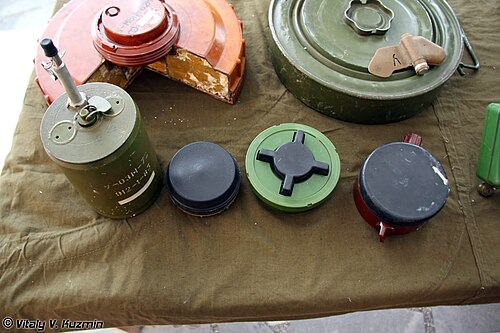
\includegraphics{../images/miny/pmn_1.jpg}
\caption{Mina PMN --- nacisgowa mina przeciwpiechotna}
\end{figure}

\subsection{Opis}\label{opis-122}

PMN (Противопехотная Мина Нажимная --- Przeciwpiechotna Mina Naciskowa)
to radziecka nacisgowa mina przeciwpiechotna z okrągłą gumową pokrywą
naciskową, opracowana w latach 50. i produkowana masowo od 1950 roku.
Jest jedną z najczęstszych min na świecie --- szacuje się ponad 10
milionów wyprodukownych egzemplarzy. Gumowa pokrywa przekazuje nacisk na
zapalnik i ładunek --- eksploduje przy nacisku 8--25 kg, wyzwalając
ładunek 200 g TNT niszczący stopę i nogę do kolana. Wersja PMN-2 (1979)
ma plastikową obudowę trudniejszą do wykrycia metalodektorem. Szeroko
stosowana w Afganistanie, Angoli, Cambodży i innych konfliktach --- i
uznawana za jedną z najbardziej ``humanitarnie problematycznych'' broni
ze względu na długotrwałe zagrożenie dla ludności cywilnej.

\subsection{Dane techniczne}\label{dane-techniczne-122}

\begin{longtable}[]{@{}ll@{}}
\toprule\noalign{}
Parametr & Wartość \\
\midrule\noalign{}
\endhead
\bottomrule\noalign{}
\endlastfoot
Typ & Nacisgowa mina przeciwpiechotna \\
Kraj produkcji & ZSRR / Rosja \\
Rok wprowadzenia & 1950 \\
Masa & 550 g \\
Masa ładunku & 200 g TNT \\
Średnica & 110 mm \\
Wysokość & 53 mm \\
Ciśnienie aktywacji & 8--25 kg \\
Długość życia & dziesiątki lat \\
\end{longtable}

\subsection{Charakterystyczne cechy
rozpoznawcze}\label{charakterystyczne-cechy-rozpoznawcze-122}

\begin{quote}
Jak odróżnić PMN od min zachodnich i PMN-2:
\end{quote}

\begin{itemize}
\tightlist
\item
  \textbf{Okrągła czarna gumowa pokrywa naciskowa --- charakterystyczny
  ``gumowy talerzyk'':} PMN ma wyraźną okrągłą czarną gumową pokrywę na
  górze; wygląda jak mały gumowy ``krążek'' z delikatnym wgłębieniem;
  żadna zachodnia mina nie wygląda dokładnie tak
\item
  \textbf{Okrągła, płaska forma --- ``blaszka w ziemi'':} cała PMN jest
  niska i okrągła; przy częściowym wyrzuceniu z ziemi lub na powierzchni
  widoczny jest okrągły ciemnozielony lub czarny krążek z gumową górą
\item
  \textbf{PMN-2 vs PMN --- PMN-2 jest bardziej ``plastikowa'' i
  jaśniejsza:} PMN-2 ma plastikową obudowę w kolorze jasnobeżowym lub
  szarym zamiast ciemnozielonego metalu PMN; łatwiejsza do odróżnienia
  po kolorze obudowy
\item
  \textbf{Bardzo płaska --- prawie niewidoczna po zakopaniu:} PMN jest
  na tyle płaska (53 mm), że po zakopaniu zostaje zaledwie kilka mm nad
  powierzchnią; trudna do wykrycia wzrokiem; widoczna jedynie po
  charakterystycznym ``zaokrąglonym wzniesieniu'' gruntu
\item
  \textbf{Brak żadnych widocznych elementów wystających --- ``czysta''
  powierzchnia:} PMN nie ma widocznych drutów, anten ani innych
  elementów nad ziemią; to odróżnia ją od min kierunkowych (MON-50) i
  min trałowanych (OZM-72) z charakterystyczną anteną
\item
  \textbf{Zakopana kilka cm --- odkrywana przez saperów z wykrywaczami
  metalu lub sondami:} PMN jest zazwyczaj zakopywana na głębokość kilku
  cm; saperzy odnajdują ją metalodektorem (PMN) lub sondą (PMN-2,
  trudniejsza do wykrycia)
\end{itemize}

\subsection{Ciekawostka}\label{ciekawostka-122}

\begin{quote}
PMN i PMN-2 są przyczyną jednego z największych humanitarnych katastrof
powojennych w historii. W Afganistanie, Angoli, Mozambiku i Kambodży
ZSRR dostarczył łącznie szacowane 10--15 milionów min PMN i PMN-2 --- z
których duża część wciąż leży w ziemi, dziesiątki lat po zakończeniu
konfliktów. Afghanistan Action (organizacja rozminowywania) szacuje, że
do 2020 roku w samym Afganistanie było wciąż 10 milionów nierozbrojonych
min. PMN jest produkt ``doskonały'' z wojskowego punktu widzenia ---
tani (ok. 3--5 dolarów za sztukę), niezawodny, długowieczny --- i
absolutnie katastrofalny z humanitarnego.
\end{quote}

\section{Mina przeciwpiechotna PMN-2}\label{mina-przeciwpiechotna-pmn-2}

\subsubsection{PMN-2 Anti-Personnel Mine \textbar{}
ПМН-2}\label{pmn-2-anti-personnel-mine-ux43fux43cux43d-2}

\begin{center}\rule{0.5\linewidth}{0.5pt}\end{center}

\begin{figure}
\centering
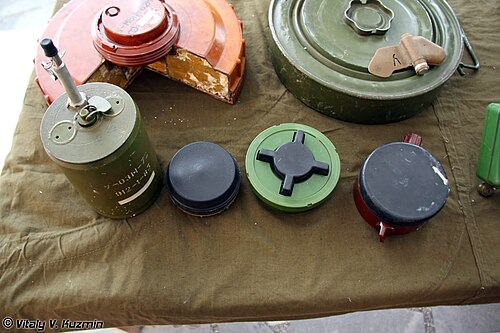
\includegraphics{../images/miny/pmn-2_1.jpg}
\caption{Mina PMN-2 --- plastikowa mina przeciwpiechotna}
\end{figure}

\subsection{Opis}\label{opis-123}

PMN-2 to radziecka modernizacja miny PMN, opracowana w 1979 roku,
wyróżniająca się obudową z prawie wyłącznie tworzywa sztucznego ---
znacznie utrudniającą wykrycie metalodektorem. Okrągła, płaska forma
(jak PMN) z gumową czarną pokrywą naciskową; aktywacja przy nacisku
5--25 kg; ładunek 100 g TNT amputuje stopę lub niszczy kończynę do
kolana. Brak metalu w obudowie (jedyną metalową częścią jest iglica
zapalnika --- kilka gramów stali) czyni PMN-2 jedną z
``najtrudniejszych'' min do wykrycia i jedną z najbardziej
problematycznych humanitarnie spośród radzieckich min. Stosowana masowo
w Afganistanie od 1979 roku, Angoli, Mozambiku, Syrii i na Ukrainie.

\subsection{Dane techniczne}\label{dane-techniczne-123}

\begin{longtable}[]{@{}ll@{}}
\toprule\noalign{}
Parametr & Wartość \\
\midrule\noalign{}
\endhead
\bottomrule\noalign{}
\endlastfoot
Typ & Nacisgowa mina przeciwpiechotna (trudna do wykrycia) \\
Kraj produkcji & ZSRR / Rosja \\
Rok wprowadzenia & 1979 \\
Masa & 400 g \\
Masa ładunku & 100 g TNT \\
Średnica & 120 mm \\
Wysokość & 54 mm \\
Ciśnienie aktywacji & 5--25 kg \\
Zawartość metalu & minimalna (iglica \textasciitilde8 g stali) \\
\end{longtable}

\subsection{Charakterystyczne cechy
rozpoznawcze}\label{charakterystyczne-cechy-rozpoznawcze-123}

\begin{quote}
Jak odróżnić PMN-2 od PMN i innych min AP:
\end{quote}

\begin{itemize}
\tightlist
\item
  \textbf{Plastikowa obudowa beżowo-szara lub jasna --- nie
  ciemnozielona jak PMN:} PMN-2 ma plastikową obudowę w kolorze
  szarobeżowym, jasnooliwkowym lub jasnym szarym; PMN jest ciemnozielona
  lub szara metaliczna; kolor jest pierwszą wskazówką odróżniającą PMN
  od PMN-2
\item
  \textbf{Gumowa czarna pokrywa naciskowa --- taka jak PMN:} oba granaty
  mają identyczną czarną gumową pokrywę naciskową; ta część jest jedynym
  ``wspólnym'' elementem wizualnym PMN i PMN-2; pokrywa ``gumowe kółko''
  jest widoczne w obu minach
\item
  \textbf{Plastikowa obudowa --- ``matowy plastik'' zamiast ``błyszczący
  metal'':} PMN-2 w dotyku i wyglądzie jest wyraźnie ``plastikowa''; PMN
  ma metaliczne wykończenie; na zdjęciach bliskich różnica tekstury jest
  widoczna; przy trzymaniu miny różnica materiału jest natychmiastowa
\item
  \textbf{Metalodetektor nie wykrywa --- efektywna tylko sondera ręczna
  lub pies saperski:} saperzy w terenie, którzy ``nie dostają sygnału''
  od metalodektora, ale sonda trafia w twardy obiekt pod ziemią --- mogą
  mieć do czynienia z PMN-2; to cecha taktyczna rozpoznawalna przez
  doświadczonych saperów
\item
  \textbf{Rozmiar identyczny z PMN --- 12 cm średnicy:} PMN i PMN-2 mają
  prawie identyczne rozmiary; odróżnienie po samym rozmiarze jest
  niemożliwe; potrzeba oceny koloru i materiału obudowy
\item
  \textbf{Bardzo długa żywotność --- aktywna przez dziesiątki lat:}
  PMN-2 z TNT jest aktywna przez dziesiątki lat; saperzy znajdowali
  sprawne PMN-2 w Angoli i Mozambiku po 30--40 latach od zakończenia
  konfliktów
\end{itemize}

\subsection{Ciekawostka}\label{ciekawostka-123}

\begin{quote}
PMN-2 jest jedną z broni, których pojawienie się w Afganistanie w 1979
roku spowodowało pilną rewizję standardów saperskich NATO. Do 1979 roku
standardowy metalodetektor był uważany za wystarczający sprzęt do
wykrywania min; po analizach afgańskich pól minowych okazało się, że
PMN-2 ``jest niewidzialna''. USA i Wielka Brytania przyspieszyły rozwój
alternatywnych technologii wykrywania (radary GPR, psy wykrywające
materiały wybuchowe) właśnie w odpowiedzi na PMN-2. To jeden z
przykładów, jak konkretna broń wymusiła zmiany w globalnych standardach
saperskich.
\end{quote}

\section{Mina przeciwpiechotna
OZM-72}\label{mina-przeciwpiechotna-ozm-72}

\subsubsection{OZM-72 Bounding Mine \textbar{}
ОЗМ-72}\label{ozm-72-bounding-mine-ux43eux437ux43c-72}

\begin{center}\rule{0.5\linewidth}{0.5pt}\end{center}

\begin{figure}
\centering
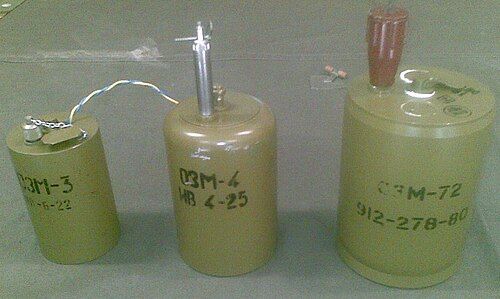
\includegraphics{../images/miny/ozm-72_1.jpg}
\caption{OZM-72 --- wyskakująca mina odłamkowa}
\end{figure}

\subsection{Opis}\label{opis-124}

OZM-72 (Осколочная Заградительная Мина-72 --- Odłamkowa Zagradzająca
Mina-72) to radziecka wyskakująca mina przeciwpiechotna odłamkowa
(bounding mine) opracowana i przyjęta do służby w 1972 roku. Gdy
aktywowana (drut lub nacisk), mina wyskakuje na wysokość 0,5--1 m nad
powierzchnię ziemi i dopiero wtedy eksploduje --- rażąc odłamkami
poziomo w promieniu do 25 m. Wybuchwanie nad ziemią czyni ją
kilkakrotnie skuteczniejszą wobec piechoty niż miny detonujące pod
ziemią (których odłamki lecą głównie w górę i są częściowo absorbowane
przez grunt). OZM-72 jest jedną z najgroźniejszych min
przeciwpiechotnych --- odpowiedzialna za bardzo wysokie straty wśród
żołnierzy i ludności cywilnej.

\subsection{Dane techniczne}\label{dane-techniczne-124}

\begin{longtable}[]{@{}ll@{}}
\toprule\noalign{}
Parametr & Wartość \\
\midrule\noalign{}
\endhead
\bottomrule\noalign{}
\endlastfoot
Typ & Wyskakująca mina odłamkowa (bounding mine) \\
Kraj produkcji & ZSRR / Rosja \\
Rok wprowadzenia & 1972 \\
Masa & 5,0 kg \\
Masa ładunku & 660 g A-IX-1 \\
Średnica cylindra & 108 mm \\
Wysokość & 172 mm \\
Zasięg odłamków & 25 m \\
Aktywacja & Drut tripwire lub nacisk \\
\end{longtable}

\subsection{Charakterystyczne cechy
rozpoznawcze}\label{charakterystyczne-cechy-rozpoznawcze-124}

\begin{quote}
Jak odróżnić OZM-72 od PMN i min kierunkowych MON:
\end{quote}

\begin{itemize}
\tightlist
\item
  \textbf{Cylindryczna forma --- ``słoik'' lub ``puszka'' stojąca w
  ziemi:} OZM-72 jest cylindryczna --- jak metalowy słoik 10 cm
  średnicy; wizualnie zupełnie inny od płaskiej PMN; po częściowym
  zakopaniu widoczny jest cylindryczny wierzch wyrastający z ziemi
\item
  \textbf{Widoczna antena lub drut tripwire wyciągnięty w teren:} OZM-72
  jest zazwyczaj aktywowana drutem tripwire --- cienki drut rozciągnięty
  przy ziemi między miną a kołkiem w odległości 5--15 m; widoczny przy
  uważnym oglądaniu terenu jako ``nitka'' przy ziemi; PMN nie ma drutu
\item
  \textbf{Charakterystyczny ``wyrzutnik'' --- mina wylatuje w górę przed
  eksplozją:} to cecha, którą można zaobserwować (przy dużym szczęściu
  lub na nagraniach): OZM-72 najpierw wyskakuje z ziemi (głośny
  ``puff''), zanim nastąpi eksplozja; odróżnia to wyraźnie od min
  detonujących natychmiast
\item
  \textbf{Zakopana głębiej niż PMN --- tylko wierzch wystaje:} OZM-72
  jest zakopana tak, że cylindryczny wierzch jest na poziomie gruntu lub
  kilka cm powyżej; saperzy szukają charakterystycznej ``puszki'' przy
  powierzchni
\item
  \textbf{Cięższa i większa od PMN --- 5 kg vs 550 g:} OZM-72 jest
  prawie 10 razy cięższa od PMN; przy transporcie i instalacji obsługa
  dźwiga wyraźnie większe i cięższe urządzenie
\item
  \textbf{Pole min OZM-72 --- wiele ``słoiczków'' rozstawionych w
  terenie z drutami między nimi:} pole min OZM-72 można rozpoznać (przy
  wiedzy i doświadczeniu) po siatce drutów tripwire między
  zainstalowanymi minami; sapera szkolony rozpoznaje to jako ``pole
  wyskakujących min''
\end{itemize}

\subsection{Ciekawostka}\label{ciekawostka-124}

\begin{quote}
OZM-72 jest wyjątkowo niebezpieczna dla rozbrajających, bo drut tripwire
może być zamontowany przez wroga tak, aby aktywacja nastąpiła
przy\ldots{} demontażu miny. Czyli saper wyciągający OZM-72 z ziemi może
aktywować dodatkowy drut zabezpieczający podłączony do innej miny. Ta
``pułapka na saperów'' była stosowana przez siły rosyjskie w Syrii i na
Ukrainie --- sprawiając, że tempo oczyszczania pól minowych dramatycznie
spada. HALO Trust (organizacja rozminowywania) szacuje, że OZM-72 należy
do najtrudniejszych i najniebezpieczniejszych min do rozbrajania spośród
wszystkich sowieckich/rosyjskich typów.
\end{quote}

\section{Mina przeciwpiechotna POM-2}\label{mina-przeciwpiechotna-pom-2}

\subsubsection{POM-2 Anti-Personnel Mine \textbar{}
ПОМ-2}\label{pom-2-anti-personnel-mine-ux43fux43eux43c-2}

\begin{center}\rule{0.5\linewidth}{0.5pt}\end{center}

\begin{figure}
\centering
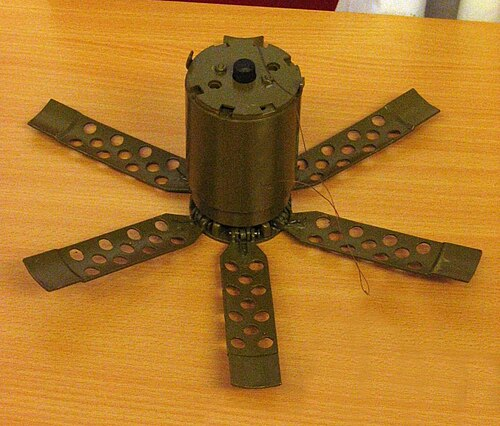
\includegraphics{../images/miny/pom-2_1.jpg}
\caption{POM-2 --- rozsypywana mina odłamkowa}
\end{figure}

\subsection{Opis}\label{opis-125}

POM-2 (Противопехотная Осколочная Мина-2 --- Przeciwpiechotna Odłamkowa
Mina-2) to radziecka rozsypywana mina przeciwpiechotna przeznaczona do
stosowania z systemów artyleryjskich i lotniczych, opracowana w latach
70.--80. Po wylądowaniu mina automatycznie rozkłada kilka cienkich
``wąsów'' (druciane tripwire) na długości 10 m każdy --- tworząc
``pajęczynę'' drutów tripwire wokół siebie; dotknięcie któregokolwiek
druta aktywuje ładunek odłamkowy niszczący w promieniu 16 m. POM-2 jest
uważana za wyjątkowo niebezpieczną --- po rozsypaniu tworzy
``niewidzialną pułapkę'' z drutami praktycznie niemożliwymi do
zauważenia w terenie roślinnym. Podlega krytyce ze względu na wysoki
odsetek zawodności autodestrukcji.

\subsection{Dane techniczne}\label{dane-techniczne-125}

\begin{longtable}[]{@{}ll@{}}
\toprule\noalign{}
Parametr & Wartość \\
\midrule\noalign{}
\endhead
\bottomrule\noalign{}
\endlastfoot
Typ & Rozsypywana mina odłamkowa z tripwire \\
Kraj produkcji & ZSRR / Rosja \\
Rok wprowadzenia & lata 80. \\
Masa & 1,4 kg \\
Masa ładunku & 140 g A-IX-1 \\
Czas autodestrukcji & 4--100 godzin \\
Zasięg rażenia & 16 m \\
Długość drutów tripwire & do 10 m (4--6 drutów) \\
Aktywacja & Drut tripwire (napięcie ok. 500 g) \\
\end{longtable}

\subsection{Charakterystyczne cechy
rozpoznawcze}\label{charakterystyczne-cechy-rozpoznawcze-125}

\begin{quote}
Jak odróżnić POM-2 od OZM-72 i PMN:
\end{quote}

\begin{itemize}
\tightlist
\item
  \textbf{Plastikowa cylindryczna forma z charakterystycznym
  ``kwiatkiem'' drutów:} POM-2 po lądowaniu rozkłada kilka cienkich
  drutów promieniście jak ``promienie gwiazdy'' lub ``płatki kwiatu''
  wokół cylindrycznej tuby; ten wzór ``mina + druty promieniście'' jest
  charakterystyczny i unikalny
\item
  \textbf{Cienkie, niemal niewidoczne druty tripwire ciągnące się 10 m
  od miny:} druty tripwire POM-2 są wyjątkowo cienkie i trudne do
  zauważenia (szczególnie w trawie lub na ziemi pokrytej liśćmi);
  saperzy szukają ich wyjątkowo ostrożnie używając lusterek i latarek
  pod niskim kątem
\item
  \textbf{Leży na powierzchni po rozsypaniu --- nie zakopywana:} jak
  PTM-3, POM-2 jest rozsypywana z powietrza i leży na powierzchni; nie
  jest zakopana; cylindryczna mina leżąca na ziemi z rozpostartymi
  drutami jest widoczna dla doświadczonego sapera
\item
  \textbf{Cylindryczna forma z ``kapslem'' i małą antenką na górze:}
  POM-2 ma charakterystyczny cylindryczny kształt z widocznym
  zapalnikiem i mechanizmem rozkładania drutów na górze; wygląda jak
  ``mała kapsuła'' z ``antenkami''
\item
  \textbf{Rozsypywana grupami --- widoczne ``konstelacje'' min na
  terenie:} po rozsypaniu przez artylerię lub śmigłowiec, POM-2 leżą w
  charakterystycznych grupach na terenie; saperzy identyfikują
  zainfekowany teren po wzorze rozsypania (jedno działo = jedna
  ``konstelacja'')
\item
  \textbf{Autodestrukcja (teoretyczna) --- praktycznie zawodna:} POM-2
  ma mechanizm autodestrukcji, ale Human Rights Watch dokumentuje
  przypadki, gdzie \textgreater{} 30\% egzemplarzy nie uległo
  autodestrukcji w czasie; teren zaminowany POM-2 jest traktowany jako
  trwałe zagrożenie
\end{itemize}

\subsection{Ciekawostka}\label{ciekawostka-125}

\begin{quote}
POM-2 jest jedną z min, którą Human Rights Watch w 2022 roku
udokumentowała jako stosowaną przez Rosję na Ukrainie w obszarach
zaludnionych --- co jest możliwym naruszeniem prawa humanitarnego. Małe,
cienkie druty tripwire POM-2 są praktycznie niewidoczne dla ludności
cywilnej, a mechanizm autodestrukcji zawodzi zbyt często, by mina mogła
być uznana za ``samolikwidującą się'' w sensie traktatowym. Ukraińskie
służby rozminowywania raportują, że oczyszczanie terenów z POM-2 jest
jednym z najtrudniejszych zadań ze względu na niewidzialność drutów i
ryzyko detonacji przy próbie usunięcia.
\end{quote}

\section{Mina-motyl PFM-1}\label{mina-motyl-pfm-1}

\subsubsection{PFM-1 Butterfly Mine \textbar{} ПФМ-1 («Попугай»,
«Бабочка»)}\label{pfm-1-butterfly-mine-ux43fux444ux43c-1-ux43fux43eux43fux443ux433ux430ux439-ux431ux430ux431ux43eux447ux43aux430}

\begin{center}\rule{0.5\linewidth}{0.5pt}\end{center}

\begin{figure}
\centering
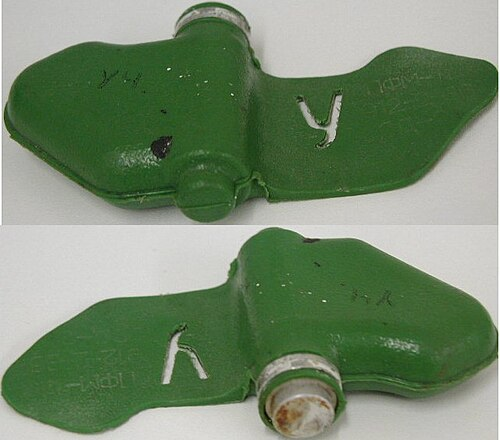
\includegraphics{../images/miny/pfm-1_1.jpg}
\caption{PFM-1 Motyl --- lotnicza mina rozsypywana}
\end{figure}

\subsection{Opis}\label{opis-126}

PFM-1 (Противопехотная Фугасная Мина-1, potocznie ``Motyl'' lub
``Papuga'') to radziecka mina lotnicza rozsypywana z powietrza,
opracowana w latach 70. i stosowana masowo w Afganistanie od 1979 roku.
Charakterystyczny kształt ``motyla'' lub ``kolibrzącej zabawki'' ---
asymetryczne plastikowe skrzydełka spowalniają opadanie i powodują
losowe lądowanie w pozycji gotowości. Mina zawiera zaledwie 37 ml
ciekłego materiału wybuchowego DMDNB (nitroestry) --- wystarczające do
odjęcia stopy lub dłoni przy aktywacji przez nacisk powyżej 4--12 kg.
Brak metalu (plastikowa obudowa) czyni ją niemal niewykrywalną
metalodektorem. Używana masowo w Afganistanie, Angoli, Mozambiku i Syrii
--- i uznawana za jedną z najbardziej ``humanitarnie problematycznych''
broni XX wieku.

\subsection{Dane techniczne}\label{dane-techniczne-126}

\begin{longtable}[]{@{}ll@{}}
\toprule\noalign{}
Parametr & Wartość \\
\midrule\noalign{}
\endhead
\bottomrule\noalign{}
\endlastfoot
Typ & Lotnicza rozsypywana mina naciskowa \\
Kraj produkcji & ZSRR / Rosja \\
Rok wprowadzenia & ok. 1979 (Afganistan) \\
Masa & 77 g \\
Masa ładunku & 37 ml DMDNB (ciekły) \\
Wymiary & 120 × 63 mm \\
Ciśnienie aktywacji & 4--12 kg \\
Czas życia aktywnej & miesiące do lat \\
Autodestrukcja & BRAK \\
\end{longtable}

\subsection{Charakterystyczne cechy
rozpoznawcze}\label{charakterystyczne-cechy-rozpoznawcze-126}

\begin{quote}
Jak odróżnić PFM-1 od innych min i ``nie pomylić z zabawką'':
\end{quote}

\begin{itemize}
\tightlist
\item
  \textbf{Charakterystyczny kształt ``skrzydlaty'' --- jak motyl lub
  helikopter z tworzywa:} PFM-1 ma unikalny asymetryczny kształt z dwoma
  ``skrzydełkami'' --- wygląda jak plastikowa zabawka, ptaszek lub liść;
  żadna inna mina nie wygląda tak; ten kształt jest absolutnym
  identyfikatorem
\item
  \textbf{Jasnozielony, oliwkowy lub beżowy kolor plastiku --- prawie
  jak zabawka:} PFM-1 jest wykonana z ciemnooliwkowego lub
  jasnozielonego twardego plastiku; na piaszczystym lub kamienistym
  terenie jest niemal niewidoczna; na trawie lub liściach wygląda jak
  kawałek plastiku lub zabawka
\item
  \textbf{Mała --- 12 × 6 cm --- można ją pomylić z ptaszkiem lub
  liściem:} PFM-1 jest mała i lekka; wśród kamieni, liści i roślinności
  jest wyjątkowo trudna do dostrzeżenia; to właśnie jej główna cecha
  ``stealth'' --- kamufluje się jako śmieć lub liść
\item
  \textbf{Brak metalu --- metalodetektor jej nie wykryje:} PFM-1 jest w
  całości plastikowa; standardowe metalodektory są przy niej
  bezużyteczne; do wykrywania potrzeba specjalnych technik (sonda, radar
  GPR, psy wyszkolone do wykrywania min)
\item
  \textbf{Leży na powierzchni --- nie zakopywana:} jak PTM-3 i POM-2,
  PFM-1 ląduje na powierzchni; nie jest zakopywana; leży na ziemi wśród
  naturalnych elementów terenu
\item
  \textbf{BRAK autodestrukcji --- może być aktywna latami:} PFM-1 nie ma
  żadnego mechanizmu autodestrukcji; ciekły materiał wybuchowy DMDNB
  może być aktywny przez miesiące lub lata; to jedna z najdłużej
  pozostających aktywnych min
\end{itemize}

\subsection{Ciekawostka}\label{ciekawostka-126}

\begin{quote}
PFM-1 ``Motyl'' stała się symbolem jednej z największych kontrowersji
humanitarnych zimnej wojny. W Afganistanie radzieckie śmigłowce Mi-8
rozsypywały miny PFM-1 mieszane z zabawkami --- bo dowódcy radzieccy
mieli nadzieję, że afghańskie dzieci będą zbierać ``kolorowe zabawki'' i
detonować miny, zmuszając rodziny do porzucenia wiosek. ONZ nigdy nie
potwierdziło oficjalnie tej taktyki mieszania z zabawkami, ale
odniesieniach afgańskich ocalałych i w dokumentacjach ICRC z lat
1980--1988 znaleziono liczne relacje o cierpieniu dzieci po zbieraniu
``motylich zabawek''. PFM-1 do dziś leży w górach Afganistanu i co roku
okalecza dzieci.
\end{quote}

\section{Mina kierunkowa MON-50}\label{mina-kierunkowa-mon-50}

\subsubsection{MON-50 Directional Mine \textbar{}
МОН-50}\label{mon-50-directional-mine-ux43cux43eux43d-50}

\begin{center}\rule{0.5\linewidth}{0.5pt}\end{center}

\begin{figure}
\centering
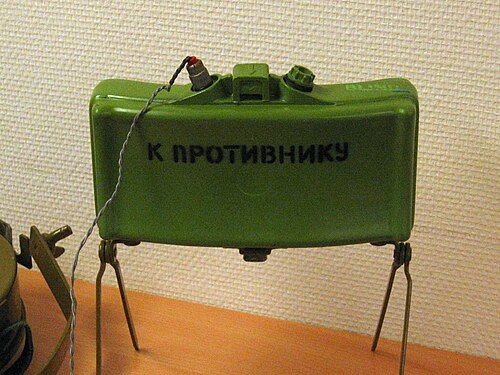
\includegraphics{../images/miny/mon-50_1.jpg}
\caption{MON-50 --- kierunkowa mina odłamkowa}
\end{figure}

\subsection{Opis}\label{opis-127}

MON-50 (Мина Осколочная Направленного действия-50 --- Mina Odłamkowa
Kierunkowa-50) to radziecka mina kierunkowa odłamkowa, odpowiednik
zachodniej M18 Claymore, opracowana w latach 60. i przyjęta do służby.
Zawiera 485 g RDX i 540 stalowych kulek 6 mm --- przy detonacji
wystrzeliwuje je łukiem 54° poziomo i 9° pionowo na odległość do 50 m
skuteczności (strefa śmierci do 60 m). MON-50 jest aktywowana
elektrycznie (kabel) lub przez zapalnik optyczny/naciskowy. Może być
montowana na kołkach lub przytwierdzona do drzew/ścian. W odróżnieniu od
PMN, MON-50 jest bronią taktyczną kontrolowaną przez żołnierza ---
zazwyczaj nie jest miną ``czekającą'', ale detonowaną zdalnie podczas
zasadzki. Szeroko stosowana w Syrii, Czeczenii i na Ukrainie.

\subsection{Dane techniczne}\label{dane-techniczne-127}

\begin{longtable}[]{@{}ll@{}}
\toprule\noalign{}
Parametr & Wartość \\
\midrule\noalign{}
\endhead
\bottomrule\noalign{}
\endlastfoot
Typ & Kierunkowa mina odłamkowa \\
Kraj produkcji & ZSRR / Rosja \\
Rok wprowadzenia & lata 60. \\
Masa & 2,0 kg \\
Masa ładunku & 485 g RDX \\
Wymiary & 230 × 150 × 85 mm \\
Liczba kulek & 540 (6 mm stal) \\
Kąt sektora rażenia & 54° (poziomo) × 9° (pionowo) \\
Strefa śmierci & do 60 m \\
Aktywacja & Elektryczna / optyczna / nacisk \\
\end{longtable}

\subsection{Charakterystyczne cechy
rozpoznawcze}\label{charakterystyczne-cechy-rozpoznawcze-127}

\begin{quote}
Jak odróżnić MON-50 od PMN i M18 Claymore:
\end{quote}

\begin{itemize}
\tightlist
\item
  \textbf{Prostokątna ``deseczka'' z wypukłą stroną --- zupełnie inny
  kształt niż okrągłe miny:} MON-50 ma charakterystyczny prostokątny
  kształt jak ``wygięta deska'' --- 23 cm × 15 cm, wypukła z przodu;
  zupełnie inny od okrągłej PMN i cylindrycznej OZM-72; ten prostokątny
  kształt jest natychmiastowym identyfikatorem
\item
  \textbf{Napis ``СТРЕЛЯЕТ В ЭТУ СТОРОНУ'' (Strzela w tę stronę) na
  wypukłej stronie:} MON-50 ma wygrawerowany napis na wypukłej stronie
  wskazujący kierunek odłamków; zachodnia M18 Claymore ma napis ``FRONT
  TOWARD ENEMY''; widok napisu cyrylicą jednoznacznie identyfikuje
  rosyjską minę
\item
  \textbf{Cztery nóżki ze skręcanymi kołkami do montażu w ziemi:} MON-50
  ma charakterystyczne cztery skośne nóżki/podpory, na których jest
  montowana --- jak ``mała deska na czterech nóżkach''; ta podstawa jest
  widoczna przy zamontowanej minie
\item
  \textbf{Kabel elektryczny lub przewód detonatora wychodzący z boku:}
  MON-50 aktywowana elektrycznie ma charakterystyczny kabel elektryczny
  wychodzący z boku ku stanowisku detonatora; widok kabla biegnącego
  przez teren to sygnał miny kierunkowej
\item
  \textbf{Montowana na drzewach, ścianach i ogrodzeniach --- nie
  zakopywana:} MON-50 często jest przymocowywana do drzew, ścian lub
  słupów zamiast zakopywania; widok ``deski przymocowanej do drzewa na
  wysokości talii'' jest charakterystyczny dla pola zasadzki z MON-50
\item
  \textbf{Bez zakopywania --- widoczna na powierzchni:} w odróżnieniu od
  PMN i OZM-72, MON-50 jest zazwyczaj widoczna (jeśli jej nie ukryto
  specjalnie); saperzy szukają jej wzrokiem, nie metalodektorem
\end{itemize}

\subsection{Ciekawostka}\label{ciekawostka-127}

\begin{quote}
MON-50 i jej zachodnia siostra M18 Claymore zostały zaprojektowane
niezależnie w tym samym czasie i działają niemal identycznie --- co jest
jednym z ciekawszych przykładów ``równoległej ewolucji'' w historii
uzbrojenia. Obie miny mają napisy skierowane do użytkownika (``strzela w
tę stronę''), bo doświadczenie pokazało, że żołnierze MYLILI strony i
detonowali je w nieodpowiednim kierunku. W czasie zimnej wojny obie
strony zakładały u siebie zdobyczne miny przeciwnika i odkryły, że mogą
używać amunicji zamiennie --- bo zapalniki elektryczne miały te same
specyfikacje napięcia i wtyki.
\end{quote}

\section{Mina kierunkowa MON-100}\label{mina-kierunkowa-mon-100}

\subsubsection{MON-100 Directional Mine \textbar{}
МОН-100}\label{mon-100-directional-mine-ux43cux43eux43d-100}

\begin{center}\rule{0.5\linewidth}{0.5pt}\end{center}

\begin{figure}
\centering
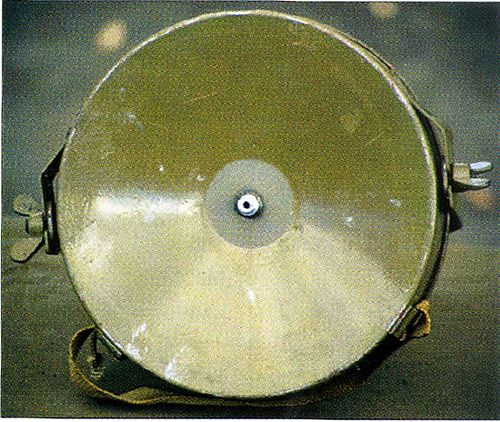
\includegraphics{../images/miny/mon-100_1.jpg}
\caption{MON-100 --- duża kierunkowa mina odłamkowa}
\end{figure}

\subsection{Opis}\label{opis-128}

MON-100 (Мина Осколочная Направленного действия-100) to radziecka duża
mina kierunkowa odłamkowa, opracowana jako ``ciężka siostra'' MON-50.
Zawiera 2000 g RDX i 400 stalowych kulek 12 mm --- znacznie większych od
kulek MON-50 (6 mm). Kąt sektora rażenia to 30° (węższy niż 54° MON-50),
ale zasięg śmiercionośny wynosi 100 m zamiast 50 m --- co daje ponad
dwukrotnie głębszą strefę rażenia. MON-100 jest przeznaczona do rażenia
celów w większej odległości i do zatrzymywania kolumn pojazdów (kulki 12
mm mogą penetrować lekkimi pancerzami). Aktywowana elektrycznie lub
przez zapalnik naciskowy/optyczny. Stosowana w zasadzkach i obronie
stałych pozycji.

\subsection{Dane techniczne}\label{dane-techniczne-128}

\begin{longtable}[]{@{}ll@{}}
\toprule\noalign{}
Parametr & Wartość \\
\midrule\noalign{}
\endhead
\bottomrule\noalign{}
\endlastfoot
Typ & Duża kierunkowa mina odłamkowa \\
Kraj produkcji & ZSRR / Rosja \\
Rok wprowadzenia & lata 70. \\
Masa & 5,0 kg \\
Masa ładunku & 2 000 g RDX \\
Wymiary & 235 × 80 mm (okrągła) \\
Liczba kulek & 400 (12 mm stal) \\
Kąt sektora rażenia & 30° (poziomo) \\
Strefa śmierci & do 100 m \\
Aktywacja & Elektryczna \\
\end{longtable}

\subsection{Charakterystyczne cechy
rozpoznawcze}\label{charakterystyczne-cechy-rozpoznawcze-128}

\begin{quote}
Jak odróżnić MON-100 od MON-50 i innych min kierunkowych:
\end{quote}

\begin{itemize}
\tightlist
\item
  \textbf{Okrągła forma ``tarczy'' lub ``fryzbee'' z wypukłością ---
  inny kształt niż prostokątny MON-50:} MON-100 ma okrągłą lub
  eliptyczną formę (nie prostokątną jak MON-50); wygląda jak okrągła
  ``tarcza'' lub ``fryzbee''; ten okrągły kształt jest pierwszym
  identyfikatorem różniącym MON-100 od MON-50
\item
  \textbf{Wyraźnie większa i cięższa od MON-50 --- 5 kg vs 2 kg:}
  MON-100 jest 2,5 razy cięższa od MON-50; przy transporcie wyraźna
  różnica masy; ``ciężka okrągła tarcza'' vs ``lekka prostokątna deska''
\item
  \textbf{Szerszy kąt 30° vs 54° MON-50 --- węższy sektor, głębszy
  zasięg:} MON-100 robi węższy but głębszy lejek rażenia; taktycznie
  przeznaczona do rażenia wąskiego pasa ale głębiej; MON-50 pokrywa
  szerszy sektor ale płycej
\item
  \textbf{Montowana nieruchomo --- ciężka do przeniesienia i
  instalacji:} ze względu na masę 5 kg, MON-100 jest zazwyczaj montowana
  stacjonarnie na stałych pozycjach; MON-50 (2 kg) jest bardziej
  ``mobilna'' i często stosowana w zasadzkach ruchomych
\item
  \textbf{Kabel elektryczny detonatora --- identyczny jak MON-50:}
  MON-100 jak MON-50 jest aktywowana elektrycznie; charakterystyczny
  kabel elektryczny wychodzący od miny; przy polu min z MON-100 widoczna
  sieć kabli biegnących do centralnego stanowiska detonacji
\item
  \textbf{Napis cyrylicą na stronie rażenia --- identycznie jak MON-50:}
  MON-100 ma napis wskazujący kierunek na stronie rażącej; cyrylica
  identyczna jak w MON-50; standardowa cecha rosyjskich min kierunkowych
\end{itemize}

\subsection{Ciekawostka}\label{ciekawostka-128}

\begin{quote}
MON-100 jest uznawana za ``myśliwską'' wersję miny kierunkowej ---
zaprojektowaną do rażenia celów w odległości 50--100 m, gdzie MON-50
jest już nieskuteczna. Na ukraińskim froncie obrońcy stosowali MON-100
jako drugą linię obrony zasadzkowej za MON-50 --- schemat: MON-50
``przywita'' pierwszą falę na 50 m, MON-100 razi podchodzące posiłki na
100 m. Ta dwupozycyjna zasadzka minowa jest zalecaną techniką w
rosyjskim i ukraińskim podręczniku saperskim. Rosja stosowała tę
technikę w Syrii do ochrony dróg zaopatrzenia przed atakami piechoty.
\end{quote}

\section{Mina przeciwpancerna TM-57}\label{mina-przeciwpancerna-tm-57}

\subsubsection{TM-57 Anti-Tank Mine \textbar{}
ТМ-57}\label{tm-57-anti-tank-mine-ux442ux43c-57}

\begin{center}\rule{0.5\linewidth}{0.5pt}\end{center}

\begin{figure}
\centering
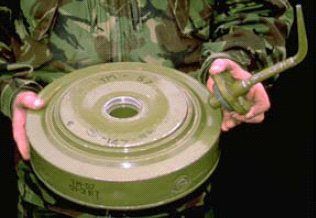
\includegraphics{../images/miny/tm-57_1.jpg}
\caption{TM-57 --- ciężka mina przeciwpancerna}
\end{figure}

\subsection{Opis}\label{opis-129}

TM-57 (Танковая Мина-57 --- Mina Czołgowa-57) to radziecka ciężka
nacisgowa mina przeciwpancerna opracowana i przyjęta do służby w 1957
roku jako następnik TM-46. Masywny ładunek 6,5 kg TNT/amatolu daje siłę
wybuchu zdolną do przebicia spodu kadłuba nawet ciężkiego czołgu; mina
szczególnie skuteczna jest wobec gąsienic i układu jezdnego. Metalowa
stalowa obudowa sprawia, że TM-57 jest wykrywalna metalodektorem --- ale
ze względu na masywną grubość (12 cm) jest trudna do minowania ręcznego.
Zapalnik MV-57 aktywuje się przy nacisku ponad 200 kg (silnik pojazdu)
lub ponad 120 kg (osie pojazdu). TM-57 jest wycofywana przez nowsze
TM-62, ale wciąż jest w magazynach i pojawia się w konfliktach.

\subsection{Dane techniczne}\label{dane-techniczne-129}

\begin{longtable}[]{@{}ll@{}}
\toprule\noalign{}
Parametr & Wartość \\
\midrule\noalign{}
\endhead
\bottomrule\noalign{}
\endlastfoot
Typ & Ciężka nacisgowa mina przeciwpancerna \\
Kraj produkcji & ZSRR \\
Rok wprowadzenia & 1957 \\
Masa & 9,0 kg \\
Masa ładunku & 6,5 kg TNT/Amatol \\
Średnica & 316 mm \\
Wysokość & 120 mm \\
Ciśnienie aktywacji & \textgreater120--200 kg \\
Obudowa & Stalowa \\
\end{longtable}

\subsection{Charakterystyczne cechy
rozpoznawcze}\label{charakterystyczne-cechy-rozpoznawcze-129}

\begin{quote}
Jak odróżnić TM-57 od TM-62 i min lżejszych:
\end{quote}

\begin{itemize}
\tightlist
\item
  \textbf{Starszy projekt --- grubsza i masywniejsza obudowa niż TM-62:}
  TM-57 jest wyraźnie bardziej masywna i grubsza od TM-62 (12 cm vs 12,8
  cm, ale TM-57 jest wyraźnie cięższa przez grubszą stalową obudowę);
  ``ciężki stalowy talerz'' to opis TM-57
\item
  \textbf{Stalowa obudowa z charakterystycznym żebrowaniem lub wzorem:}
  TM-57 ma ciemnostalową obudowę z charakterystycznym wzorem żeber lub
  przetłoczeń na górnej płycie; TM-62 ma gładką lub mniej wyraźnie
  żebrowaną powierzchnię
\item
  \textbf{Zapalnik MV-57 ze specyficznym kapturkiem:} zapalnik TM-57 ma
  charakterystyczny kapturek i sposób montażu; znający miny saper
  rozróżnia zapalniki TM-57 i TM-62 po formie zapalnika
\item
  \textbf{Starsza technologia --- bardziej ``archaiczny'' wygląd od
  TM-62:} TM-57 wygląda jak broń z lat 50. --- co jest zgodne z prawdą;
  grubsze połączenia, mniej ergonomiczne detale, inne przetłoczenia;
  TM-62 jest z lat 60. i wyraźnie ``nowocześniejsza''
\item
  \textbf{Masa 9 kg --- podobna do TM-62 (9,5--10 kg) --- ciężka mina
  AT:} przy transportowaniu miny saper czuje ciężar zbliżony do TM-62;
  odróżnienie po samej masie jest trudne --- potrzeba oglądania obudowy
\item
  \textbf{Coraz rzadsza --- wypierana przez TM-62 w aktywnych stockach:}
  TM-57 pojawia się głównie w starych magazynach lub na polach minowych
  z lat 60.--80.; na nowych polach minowych dominuje TM-62; ``stara
  mina'' jest identyfikatorem epoki zakładania pola
\end{itemize}

\subsection{Ciekawostka}\label{ciekawostka-129}

\begin{quote}
TM-57 była pierwszą radziecką miną przeciwpancerną wystarczająco potężną
do niezawodnego zniszczenia ciężkich czołgów amerykańskich M60 i M48.
Wcześniejsza TM-46 była projektowana pod czołgi WWII i w testach z lat
50. okazała się niewystarczająca wobec nowego ciężkiego opancerzenia.
TM-57 z 6,5 kg materiału wybuchowego przebijała spód M60 i niszczyła
przedział silnikowy. To wymaganie taktyczne --- ``mina musi zniszczyć
M60'' --- dyktowało parametry całej rodziny TM-57/TM-62 i jest
eleganckim przykładem, jak konkretne zagrożenie operacyjne kształtuje
parametry broni.
\end{quote}

\section{Mina przeciwpancerna TM-62M}\label{mina-przeciwpancerna-tm-62m}

\subsubsection{TM-62M Anti-Tank Mine \textbar{}
ТМ-62М}\label{tm-62m-anti-tank-mine-ux442ux43c-62ux43c}

\begin{center}\rule{0.5\linewidth}{0.5pt}\end{center}

\begin{figure}
\centering
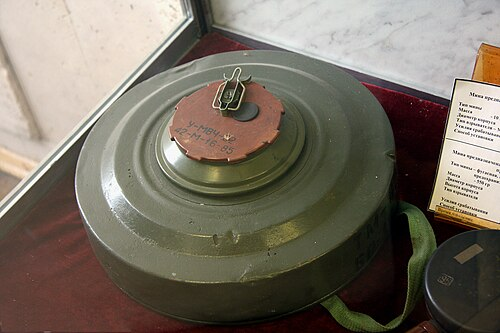
\includegraphics{../images/miny/tm-62_1.jpg}
\caption{TM-62M --- mina przeciwpancerna}
\end{figure}

\subsection{Opis}\label{opis-130}

TM-62M (Танковая Мина-62М --- Mina Czołgowa-62M) to radziecka nacisgowa
mina przeciwpancerna z metalową obudową, opracowana w 1962 roku jako
modernizacja TM-57. Jest jedną z najszerzej stosowanych min
przeciwpancernych na świecie --- produkowana w licznych wariantach
(TM-62B z drewnianą obudową, TM-62P z plastikową) i eksportowana do
ponad 50 krajów. Okrągła obudowa z naciągową płytą --- wybucha przy
nacisku ponad 200--500 kg, co powoduje eksplozję 7--8 kg TNT niszczącą
gąsienice, koła lub podwozie pojazdu opancerzonego. Wersja TM-62P2 i
TM-62P3 mają plastikową obudowę trudną do wykrycia metalodektorem.
Szeroko stosowana na Ukrainie.

\subsection{Dane techniczne}\label{dane-techniczne-130}

\begin{longtable}[]{@{}ll@{}}
\toprule\noalign{}
Parametr & Wartość \\
\midrule\noalign{}
\endhead
\bottomrule\noalign{}
\endlastfoot
Typ & Nacisgowa mina przeciwpancerna \\
Kraj produkcji & ZSRR / Rosja \\
Rok wprowadzenia & 1962 \\
Masa & 9,5--10 kg \\
Masa ładunku & 7,0--8,0 kg TNT \\
Średnica & 320 mm \\
Wysokość & 128 mm \\
Ciśnienie aktywacji & 200--500 kg \\
Wersje & TM-62M (metal), TM-62B (drewno), TM-62P (plastik) \\
\end{longtable}

\subsection{Charakterystyczne cechy
rozpoznawcze}\label{charakterystyczne-cechy-rozpoznawcze-130}

\begin{quote}
Jak odróżnić TM-62M od PMN i PTM-3:
\end{quote}

\begin{itemize}
\tightlist
\item
  \textbf{Duży okrągły ``talerz'' --- wyraźnie większy od min
  przeciwpiechotnych:} TM-62M ma średnicę 32 cm --- wyraźnie większa od
  okrągłych min przeciwpiechotnych PMN (11 cm); ``duży okrągły talerz''
  to natychmiastowy identyfikator miny przeciwpancernej
\item
  \textbf{Wyraźna płyta naciskowa z wgłębieniem pośrodku:} na górze
  TM-62M widoczna jest okrągła płyta naciskowa z charakterystycznym
  wgłębieniem lub wzniosłością pośrodku; to element aktywujący przez
  nacisk pojazdu; charakterystyczny wygląd płyty naciskowej
\item
  \textbf{Stalowa (TM-62M), drewniana (TM-62B) lub plastikowa (TM-62P)
  obudowa --- różne kolory:} TM-62M metalowa jest ciemnozielona; TM-62B
  drewniana ma jasnobeżowy kolor surowego drewna; TM-62P plastikowa jest
  szarawobiała lub oliwkowa; kolor obudowy zależy od wersji
\item
  \textbf{Zakopywana głębiej niż miny przeciwpiechotne --- do 10 cm pod
  powierzchnią:} TM-62M jest zakopywana głębiej; saperzy szukają jej na
  głębokości 10 cm; nierówności gruntu i charakterystyczne ślady
  zakopywania (świeżo spulchniona ziemia) mogą ją zdradzić
\item
  \textbf{Waga 10 kg --- wyraźnie cięższa od min przeciwpiechotnych:}
  TM-62M waży 10 kg; PMN waży 550 g; przy transporcie w plecaku lub
  wozie amunicyjnym wyraźna różnica w ciężarze; pole min TM-62M jest
  zakładane przez pojazdy lub wielu żołnierzy
\item
  \textbf{Okrągły kształt z dwiema symetrycznie rozmieszczonymi dziurami
  (zapalniki):} TM-62M ma dwie otwory na zapalniki umieszczone
  symetrycznie po obu stronach płyty naciskowej; te otwory są
  charakterystyczną cechą wizualną przy oglądaniu miny z góry
\end{itemize}

\subsection{Ciekawostka}\label{ciekawostka-130}

\begin{quote}
TM-62P (plastikowa) jest uważana za jeden z największych problemów
humanitarnych związanych z rozminowywaniem, bo wykrywacz metali jej nie
wykrywa --- a sonda ręczna jest powolna i niebezpieczna. Na polach bitew
Angoli, Mozambiku i Kambodży TM-62P leży w ziemi od 40--50 lat i wciąż
jest aktywna --- bo TNT nie ulega degradacji. Szacuje się, że w samej
Angoli w ziemi leży 10--15 milionów TM-62P i PMN-2. HALO Trust i inne
organizacje rozminowywania twierdzą, że przy obecnym tempie pracy pełne
rozminowanie Angoli zajmie kolejne 20--30 lat.
\end{quote}

\section{Mina przeciwpancerna PTM-3}\label{mina-przeciwpancerna-ptm-3}

\subsubsection{PTM-3 Anti-Tank Mine \textbar{}
ПТМ-3}\label{ptm-3-anti-tank-mine-ux43fux442ux43c-3}

\begin{center}\rule{0.5\linewidth}{0.5pt}\end{center}

\begin{figure}
\centering
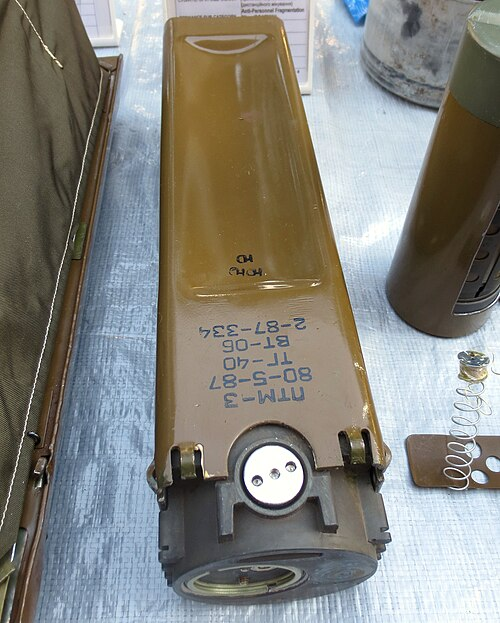
\includegraphics{../images/miny/ptm-3_1.jpg}
\caption{PTM-3 --- rozsypywana mina przeciwpancerna}
\end{figure}

\subsection{Opis}\label{opis-131}

PTM-3 (Противотанковая Мина-3) to radziecka rozsypywana mina
przeciwpancerna kalibru 275 mm, opracowana i przyjęta do służby w 1978
roku do stosowania z systemów minowania artyleryjskiego i lotniczego. W
odróżnieniu od TM-62, PTM-3 nie jest zakopywana ręcznie --- jest
rozsypywana przez działa artyleryjskie (system UMZ), śmigłowce lub
samoloty i po kontakcie z ziemią ``samoczynnie'' przyjmuje pozycję
gotowości. Ma zapalnik z mechanizmem autodestrukcji (po 16--24 godzinach
lub 40 dniach w zależności od ustawienia) --- co częściowo redukuje
długotrwałe zagrożenie humanitarne. PTM-3 jest miną przeciwpancerną
kumulacyjną --- skierowana dnem ku górze, wybucha pod pojazdem
eksplodując w stronę spodu kadłuba.

\subsection{Dane techniczne}\label{dane-techniczne-131}

\begin{longtable}[]{@{}ll@{}}
\toprule\noalign{}
Parametr & Wartość \\
\midrule\noalign{}
\endhead
\bottomrule\noalign{}
\endlastfoot
Typ & Rozsypywana mina przeciwpancerna (FASCAM) \\
Kraj produkcji & ZSRR / Rosja \\
Rok wprowadzenia & 1978 \\
Masa & 1,6 kg \\
Masa ładunku & 1,0 kg RDX \\
Średnica & 275 mm \\
Czas autodestrukcji & 16--24 h lub 40 dni (ustawialny) \\
Aktywacja & Magnetyczna / naciskowa \\
Przenikanie pancerza & 100--120 mm stali \\
\end{longtable}

\subsection{Charakterystyczne cechy
rozpoznawcze}\label{charakterystyczne-cechy-rozpoznawcze-131}

\begin{quote}
Jak odróżnić PTM-3 od TM-62 i zakopywanych min AP:
\end{quote}

\begin{itemize}
\tightlist
\item
  \textbf{Płaska, dyskoidalna forma --- ``frisbee'' lub ``latający
  talerz'':} PTM-3 ma charakterystyczny płaski, okrągły kształt jak dysk
  lub spodek latający; po wylądowaniu leży poziomo na ziemi; całkowicie
  inny od cylindrycznej TM-62 i prostokątnej MON-50
\item
  \textbf{Leży na powierzchni --- nie zakopywana:} PTM-3 jest
  rozsypywana z powietrza lub artylerii i leży na powierzchni gruntu;
  nie jest zakopywana jak TM-62; widoczna mina ``disk'' leżąca na ziemi
  to charakterystyczny widok pola zaminowanego PTM-3
\item
  \textbf{Małe ``nóżki'' lub ``stopy'' stabilizujące przy lądowaniu:}
  PTM-3 ma małe elementy stabilizujące, które po lądowaniu ustalają
  właściwą orientację dnem ku górze (tak aby głowica kumulacyjna była
  skierowana w spód pojazdu); te stabilizatory są widoczne przy bliskim
  oglądaniu
\item
  \textbf{Wyraźnie mniejsza od TM-62 --- 275 mm vs 320 mm, 1,6 kg vs 10
  kg:} PTM-3 jest lżejsza i mniejsza od TM-62; przy trzymaniu ---
  wyraźnie lżejsza; rozmiar ``frisbee'' vs ``duży talerz'' TM-62
\item
  \textbf{Często widoczna w grupach po rozsypaniu artyleryjskim:} PTM-3
  jest rozsypywana grupami przez jedno działo lub jeden pasaż śmigłowca;
  na terenie zaminowanym widać je w grupach ``kilku-kilkunastu dysków''
  w promieniu kilkudziesięciu metrów
\item
  \textbf{Autodestrukcja po określonym czasie --- (teoretycznie)
  ograniczone zagrożenie trwałe:} PTM-3 ma mechanizm autodestrukcji po
  16--40 dniach; jednak ten mechanizm często zawodzi, pozostawiając
  aktywne miny na długo; zachodnie organizacje rozminowywania traktują
  PTM-3 jako potencjalnie trwałe zagrożenie
\end{itemize}

\subsection{Ciekawostka}\label{ciekawostka-131}

\begin{quote}
PTM-3 jest jedną z min, których użycie w Syrii i na Ukrainie
dokumentowały organizacje Human Rights Watch i Landmine Monitor,
wskazując, że mimo mechanizmu autodestrukcji, znaczna część tych min
pozostaje aktywna długo po upływie zadeklarowanego czasu. Rosja,
podobnie jak Ukraina, nie jest sygnatariuszem Traktatu Ottawskiego
(zakaz min przeciwpiechotnych) --- i obie strony używają różnych typów
min bez ograniczeń traktatowych. PTM-3 jest ``legalną'' bronią wojskową
w rosyjskiej doktrynie, stosowaną masowo do tworzenia szybkich pól
minowych przed natarciem lub wycofywaniem.
\end{quote}

\section{Mina kasetowa KPOM-2}\label{mina-kasetowa-kpom-2}

\subsubsection{KPOM-2 Cluster Submunition \textbar{}
КПОМ-2}\label{kpom-2-cluster-submunition-ux43aux43fux43eux43c-2}

\begin{center}\rule{0.5\linewidth}{0.5pt}\end{center}

\begin{figure}
\centering
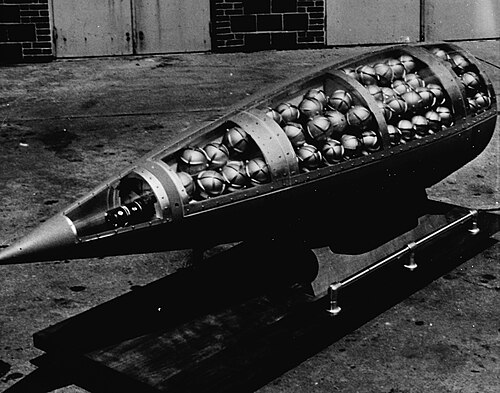
\includegraphics{../images/miny/kpom-2_1.jpg}
\caption{KPOM-2 --- kasetowy element minowy}
\end{figure}

\subsection{Opis}\label{opis-132}

KPOM-2 (Кассетный Противопехотный Осколочный Минный элемент-2) to
rosyjski element minowy kasetowy --- mały submunition odłamkowy
rozsypywany z rakiet artyleryjskich wieloprowadnicowych (BM-21 Grad,
BM-30 Smierć) lub bomb lotniczych kasetowych. Każda rakieta Grad może
przenosić dziesiątki elementów KPOM-2, które po wyrzuceniu rozsypują się
nad obszarem docelowym i po kontakcie z ziemią natychmiast aktywują się
--- tworząc pole mini-min w promieniu kilkudziesięciu metrów. KPOM-2 ma
zapalnik uderzeniowy i mechanizm autodestrukcji (zazwyczaj zawodny).
Bardzo trudna do wykrycia i rozbrojenia ze względu na mały rozmiar.
Stosowana masowo w Syrii i na Ukrainie; dokumentowana przez Human Rights
Watch jako zagrożenie dla ludności cywilnej.

\subsection{Dane techniczne}\label{dane-techniczne-132}

\begin{longtable}[]{@{}ll@{}}
\toprule\noalign{}
Parametr & Wartość \\
\midrule\noalign{}
\endhead
\bottomrule\noalign{}
\endlastfoot
Typ & Kasetowy submunition przeciwpiechotny \\
Kraj produkcji & Rosja \\
Dostarczanie & Rakiety BM-21 Grad, BM-30 Smierć \\
Masa & ok. 0,5 kg \\
Ładunek & ok. 40--60 g materiału wybuchowego \\
Zasięg rażenia & kilka metrów \\
Autodestrukcja & Teoretyczna (często zawodna) \\
Aktywacja & Uderzeniowa \\
\end{longtable}

\subsection{Charakterystyczne cechy
rozpoznawcze}\label{charakterystyczne-cechy-rozpoznawcze-132}

\begin{quote}
Jak odróżnić KPOM-2 od innych submunitions i granatów:
\end{quote}

\begin{itemize}
\tightlist
\item
  \textbf{Bardzo mały rozmiar --- ``miniaturowy granat'' leżący na
  ziemi:} KPOM-2 jest mały i lekki; po rozsypaniu leży na ziemi wśród
  innych odłamków i śmieci wojennych; łatwo pomylić z kawałkiem metalu,
  kamieniem lub śmieciem
\item
  \textbf{Charakterystyczny cylindryczny lub kanciasty kształt ze
  stabilizatorem:} KPOM-2 ma małe ``ogonki'' lub stabilizatory
  zapewniające prawidłową orientację przy opadaniu; te małe
  stabilizatory są widoczne przy bliskim oglądaniu
\item
  \textbf{Różnobarwne --- zielone, szare lub żółtawe --- bez wyraźnego
  oznakowania:} KPOM-2 nie ma wyraźnych oznaczeń kolorystycznych
  widocznych z odległości; wygląda jak ``mały kawałek sprzętu
  wojskowego'' bez wskazania, co to jest
\item
  \textbf{Rozsypane grupami po ataku artyleryjskim --- ``konstelacja''
  małych obiektów:} po ataku Gradem lub Smierczem z głowicami kasetowymi
  teren jest pokryty grupami KPOM-2; saperzy identyfikują ``pole
  submunitions'' po charakterystycznym wzorze rozsypania wielu małych
  obiektów
\item
  \textbf{Niewykrywalne wzrokiem po zamarznięciu lub przysypaniu
  śniegiem/błotem:} na Ukrainie zimą 2022--2023 KPOM-2 pokryte śniegiem
  były niewidoczne; wiosną topnienie śniegu ``ujawniało'' pole min,
  które tam przez całą zimę leżało
\item
  \textbf{Zawodna autodestrukcja --- pozostają aktywne długo po ataku:}
  jak PFM-1 i POM-2, KPOM-2 ma mechanizm autodestrukcji, który często
  zawodzi; raport Human Rights Watch z 2022 roku dokumentuje KPOM-2
  aktywne tygodnie po ataku
\end{itemize}

\subsection{Ciekawostka}\label{ciekawostka-132}

\begin{quote}
KPOM-2 i inne submunitions kasetowe są tematem Konwencji o amunicji
kasetowej (2008), którą podpisało ponad 110 państw --- ale nie Rosja ani
Ukraina. Kiedy w 2023 roku USA dostarczyły Ukrainie amunicję kasetową
(do armat M777 i haubic M109), wywołało to ogromną debatę --- bo Ukraina
używała jej do rażenia rosyjskich pozycji, ale Rosja wciąż stosuje
KPOM-2 i inne submunitions na ukraińskim terytorium cywilnym. Human
Rights Watch dokumentuje, że obie strony używają submunitions kasetowych
--- ale Rosja robi to na terenach cywilnych wielokrotnie częściej i na
większą skalę.
\end{quote}

\section{System minowania UMZ}\label{system-minowania-umz}

\subsubsection{UMZ Scatterable Mine System \textbar{} УМЗ (Универсальный
Минный
Заградитель)}\label{umz-scatterable-mine-system-ux443ux43cux437-ux443ux43dux438ux432ux435ux440ux441ux430ux43bux44cux43dux44bux439-ux43cux438ux43dux43dux44bux439-ux437ux430ux433ux440ux430ux434ux438ux442ux435ux43bux44c}

\begin{center}\rule{0.5\linewidth}{0.5pt}\end{center}

\begin{figure}
\centering
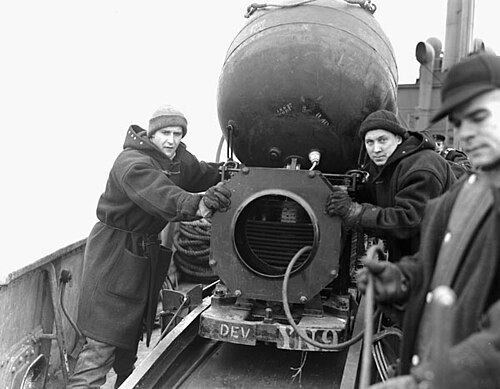
\includegraphics{../images/miny/umz_1.jpg}
\caption{UMZ --- naziemny system rozsypywania min}
\end{figure}

\subsection{Opis}\label{opis-133}

UMZ (Универсальный Минный Заградитель --- Universalny Minny Zagraditiel
--- Powszechny Systemu Minowania) to radziecko-rosyjski system
rozsypywania min z pojazdów naziemnych, opracowany w latach 70. i
przyjęty do służby w 1978 roku. Montowany na ciężarówce (najczęściej
Ural-375D lub ZiL-131), pozwala na szybkie minowanie terenu w ruchu ---
pojazd jadący z prędkością 30--40 km/h rozsypuje miny z pojemników
zamontowanych z tyłu. Jeden pojazd może zaminować pas terenu 1--1,5 km
długości i 80--100 m szerokości w ciągu kilku minut. UMZ rozsypuje miny
PTM-3 (przeciwpancerne), POM-2 (przeciwpiechotne) lub ich kombinacje.
Stosowany masowo w Syrii i na Ukrainie.

\subsection{Dane techniczne}\label{dane-techniczne-133}

\begin{longtable}[]{@{}ll@{}}
\toprule\noalign{}
Parametr & Wartość \\
\midrule\noalign{}
\endhead
\bottomrule\noalign{}
\endlastfoot
Typ & Naziemny system rozsypywania min \\
Kraj produkcji & ZSRR / Rosja \\
Rok wprowadzenia & 1978 \\
Platforma & Ural-375D lub ZiL-131 \\
Pojemność & 8 pojemników po 30 min (240 min łącznie) \\
Prędkość minowania & 30--40 km/h \\
Czas minowania pasa 1 km & ok. 2 minuty \\
Szerokość pasa min & 80--100 m \\
Typy min & PTM-3 (PT) / POM-2 (PP) / mieszane \\
\end{longtable}

\subsection{Charakterystyczne cechy
rozpoznawcze}\label{charakterystyczne-cechy-rozpoznawcze-133}

\begin{quote}
Jak odróżnić UMZ od zwykłej ciężarówki i innych systemów minowania:
\end{quote}

\begin{itemize}
\tightlist
\item
  \textbf{Charakterystyczne metalowe pojemniki-zasobniki na pace
  ciężarówki:} UMZ ma charakterystyczne 8 prostokątnych metalowych
  pojemników (zasobniki na miny) zamontowanych na pace ciężarówki; ta
  ``rzędowa'' konfiguracja pojemników na tyle pojazdu jest widoczna z
  daleka i odróżnia UMZ od zwykłej ciężarówki
\item
  \textbf{Ciężarówka Ural lub ZiL z charakterystycznym sprzętem z tyłu
  --- ``coś wyrzuca'':} UMZ w działaniu widoczny jest jako ciężarówka
  pozostawiająca za sobą ``deszcz'' min padających na ziemię; ta
  wizualna cecha --- pojazd ``rozsypujący przedmioty'' --- jest
  rozpoznawalna na zdjęciach lotniczych i nagraniach
\item
  \textbf{Przewody sterowania i kable widoczne między pojemnikami:}
  zestaw UMZ ma charakterystyczne kable i przewody łączące pojemniki z
  centralnym mechanizmem wyrzutu; ta sieć kabli na pace ciężarówki jest
  widoczna przy bliskim oglądaniu
\item
  \textbf{Rozsypane miny PTM-3 lub POM-2 za przejazdem pojazdu:} efektem
  działania UMZ jest ``pole dyskoidalnych min PTM-3 lub spaghetti drutów
  POM-2'' na drodze przejazdu; zaminowany teren po przejściu UMZ jest
  rozpoznawalny po wzorze rozsypania min (równoległy pas)
\item
  \textbf{Zdjęcia satelitarne lub dronowe --- widoczny pas zaminowany:}
  na nagraniach dronem lub zdjęciach satelitarnych (po wyjściu UMZ)
  widoczny jest charakterystyczny pas terenu o innej fakturze ---
  ``posypany'' obiektami PTM-3 lub innymi elementami
\item
  \textbf{Szybkie tworzenie pól minowych --- UMZ znika po kilku
  minutach:} specyfika UMZ to szybkość; żołnierze obserwujący teren
  widzą, że ``ciężarówka przejechała i zniknęła''; zaminowany teren
  pojawia się błyskawicznie, bez długotrwałej pracy saperów w ziemi
\end{itemize}

\subsection{Ciekawostka}\label{ciekawostka-133}

\begin{quote}
UMZ był jedną z pierwszych broni masowego zaminowania, którą Zachód
udokumentował na Ukrainie w 2022 roku. Nagrania drona pokazały pojazdy
UMZ szybko zaminowujące drogi i pola przed rosyjskim wycofaniem z obwodu
kijowskiego. Tempo zaminowania zaskoczyło ukraińskich saperów --- w
ciągu jednej nocy jedna ciężarówka UMZ może zaminować kilka kilometrów
drogi lub terenu, tworząc barierę minową niemożliwą do szybkiego
oczyszczenia. Ukraina szacuje, że 30--40\% jej terytorium zajętego przez
Rosję jest zaminowane --- a UMZ i śmigłowcowe systemy rozsypywania
odpowiadają za większość nowych min zakładanych od 2022 roku.
\end{quote}

\section{Mina przeciwpancerna VS-50}\label{mina-przeciwpancerna-vs-50}

\subsubsection{VS-50 Anti-Personnel Mine \textbar{}
ВС-50}\label{vs-50-anti-personnel-mine-ux432ux441-50}

\begin{center}\rule{0.5\linewidth}{0.5pt}\end{center}

\begin{figure}
\centering
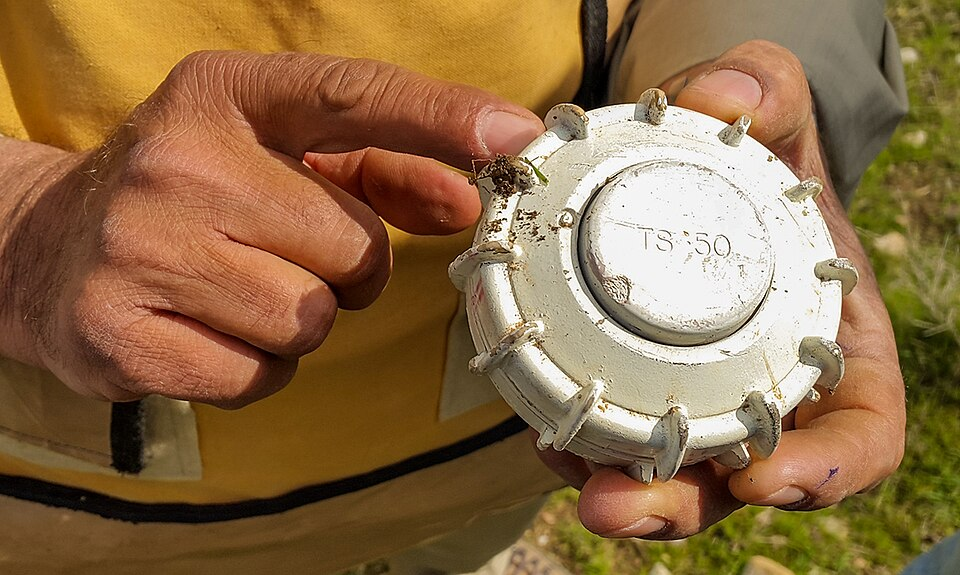
\includegraphics{../images/miny/vs-50_1.jpg}
\caption{VS-50 --- mina nacisgowa plastikowa}
\end{figure}

\subsection{Opis}\label{opis-134}

VS-50 to włoska mina przeciwpancerna (produkowana przez Valsella
Meccanotecnica) szeroko eksportowana i stosowana przez różne strony
konfliktów --- w tym Rosję i siły rosyjskie w Syrii i Czeczenii. Choć
nie jest rosyjskiej produkcji, jest często confiscated i stosowana przez
rosyjskie siły zbrojne i siły powiązane z Rosją. Plastikowa obudowa z
prawie zerową zawartością metalu czyni ją niemal niewykrywalną
metalodektorem. Aktywowana przez nacisk powyżej 8 kg --- eksplozja 40 g
materiału wybuchowego amputuje stopę lub niszczy kończynę dolną. Pojawia
się regularnie na terenach kontrolowanych przez siły rosyjskie i
prorosyjskie w Syrii i Donbasie.

\subsection{Dane techniczne}\label{dane-techniczne-134}

\begin{longtable}[]{@{}ll@{}}
\toprule\noalign{}
Parametr & Wartość \\
\midrule\noalign{}
\endhead
\bottomrule\noalign{}
\endlastfoot
Typ & Mina naciskowa (głównie przeciwpiechotna) \\
Kraj produkcji & Włochy (Valsella) \\
Masa & 185 g \\
Masa ładunku & 40 g PETN \\
Średnica & 90 mm \\
Wysokość & 45 mm \\
Ciśnienie aktywacji & 8 kg \\
Zawartość metalu & prawie zerowa \\
\end{longtable}

\subsection{Charakterystyczne cechy
rozpoznawcze}\label{charakterystyczne-cechy-rozpoznawcze-134}

\begin{quote}
Jak odróżnić VS-50 od PMN i min zachodnich:
\end{quote}

\begin{itemize}
\tightlist
\item
  \textbf{Bardzo mała i płaska --- mniejsza od PMN:} VS-50 ma tylko 90
  mm średnicy i 45 mm wysokości; wyraźnie mniejsza od PMN (110 mm, 53
  mm); ``miniaturowy krążek'' przy porównaniu
\item
  \textbf{Żółty lub beżowy plastik --- ``jasny kolor'' odróżnia od
  ciemnej PMN:} VS-50 jest zazwyczaj jasnobeżowa lub żółtawa; PMN jest
  ciemnozielona lub szara; kolor jest pierwszym identyfikatorem
  różniącym obie miny
\item
  \textbf{Włoskie oznaczenia lub ``Valsella'' na obudowie:} na VS-50
  czasem widoczne są oznaczenia producenta lub kraju; cyrylica nie
  pojawia się na VS-50; to oznaczenie jest identyfikatorem zachodniego
  producenta
\item
  \textbf{Niemal ``niewidoczna'' dla metalodektora:} VS-50 jest tak
  ``plastikowa'', że metalodetektor jej nie wykrywa; saperzy traktują ją
  jak PMN-2 --- wymagającą sondy lub specjalnych technik
\item
  \textbf{Kontekst użycia --- zdobyczna lub dostarczona przez
  pośredników:} VS-50 w rękach sił rosyjskich lub prorosyjskich jest
  zawsze ``zdobyczna'' lub ``kupiona przez pośredników''; nie jest
  oficjalnie produkowana w Rosji; jej obecność na polu walki sugeruje
  dywersję logistyki lub eksport przez kraje trzecie
\item
  \textbf{Płaski kształt ``guzika'' --- bez żadnych widocznych elementów
  zewnętrznych:} VS-50 z góry wygląda jak gładki okrągły ``guzik'' bez
  żadnych sterczących elementów; PMN ma wyraźną gumową pokrywę; VS-50
  jest gładka i ``czysta''
\end{itemize}

\subsection{Ciekawostka}\label{ciekawostka-134}

\begin{quote}
VS-50 jest paradoksalnym symbolem globalnego handlu bronią --- mina
zaprojektowana we Włoszech, produkowana komercyjnie dla ``rynków
eksportowych'', trafiła do rąk stron konfliktów, których Włochy nigdy
nie zamierzały wspierać. Human Rights Watch w raportach z lat 90. i
2000. dokumentowała VS-50 w rękach ugrupowań zbrojnych w Angoli,
Somalii, Syrii --- i przy każdym takim odkryciu Valsella zapewniała, że
``nie sprzedawała ich bezpośrednio''. Cały globalny handel minami
przeciwpiechotnymi był w dużej mierze ``nieintencjonalny'' --- miny
kupione legalnie przez jedno państwo trafiały przez pośredników do
aktora niepaństwowego lub wroga. To jeden z powodów, dla których Traktat
Ottawski zakazał całej klasy broni, a nie tylko konkretnych
użytkowników.
\end{quote}

\end{document}
